\documentclass[12pt, fleqn, openany]{studyGuide}
\setstretch{1.4}
\enableInlineReview
\renewcommand{\VMBookTitle}{Graphical Questions Review}
\renewcommand{\VMBookSubtitle}{Grade 7 --- Bank: 2 --- Chapter: all --- Graphical Questions}
\renewcommand{\VMFooterURL}{https://viewmath.com/grade7}
\renewcommand{\VMFooterURLDisplay}{ViewMath.com/Grade7}
\begin{document}

\begin{center}
\begin{tcolorbox}[
	enhanced,
	colback=white,
	colframe=funTeal!60,
	boxrule=1.5pt,
	arc=10pt,
	outer arc=10pt,
	width=0.9\linewidth,
	halign=center,
	top=5mm, bottom=5mm,
]
	{\Large\bfseries\sffamily\color{funTealDark}Graphical Questions}\\[2mm]
	{\large\sffamily\color{funGrayDark}Grade 7 --- Bank: 2 --- Chapter: all --- Graphical Questions}\\[2mm]
	{\normalsize\sffamily\color{funGrayDark}Audit visual elements below}
\end{tcolorbox}
\end{center}

\newpage
\section*{1-1-q23 \hfill \normalsize\texttt{tests\_questions\_bank\_2/topics/ch01-01-unit-rates-with-fractions.tex}}
\begin{practiceQuestion}{1-1-q23}{gmc}
\begin{questionText}
The bar graph below shows the distance two runners covered in $\frac{1}{3}$ hour.

\begin{center}
\begin{tikzpicture}[scale=0.8]
  \draw[thick,->] (0,0) -- (0,4.5) node[above]{\small Miles};
  \draw[thick,->] (0,0) -- (5,0);
  \fill[funBlue] (0.5,0) rectangle (2,3);
  \fill[funOrange] (2.5,0) rectangle (4,2.5);
  \node[below] at (1.25,0) {\small Runner A};
  \node[below] at (3.25,0) {\small Runner B};
  \foreach \y/\lab in {1/\frac{1}{4},2/\frac{1}{2},3/\frac{3}{4},4/1}
    \draw (-0.1,\y) -- (0.1,\y) node[left=4pt] {$\lab$};
\end{tikzpicture}
\end{center}

Which runner has the faster speed in miles per hour?
\end{questionText}
\choiceA{Runner A at $2\frac{1}{4}$ mph}
\choiceB{Runner B at $1\frac{7}{8}$ mph}
\choiceC{Runner A at $\frac{1}{4}$ mph}
\choiceD{Runner B at $1\frac{1}{2}$ mph}
\correctAnswer{A}
\explanation{From the graph, Runner A covers $\frac{3}{4}$ mile and Runner B covers about $\frac{5}{8}$ mile in $\frac{1}{3}$ hour. Runner A: $\frac{3}{4} \div \frac{1}{3} = \frac{3}{4} \times 3 = \frac{9}{4} = 2\frac{1}{4}$ mph. Runner B: $\frac{5}{8} \div \frac{1}{3} = \frac{5}{8} \times 3 = \frac{15}{8} = 1\frac{7}{8}$ mph. Runner A is faster.}
\end{practiceQuestion}

\newpage
\section*{1-1-q24 \hfill \normalsize\texttt{tests\_questions\_bank\_2/topics/ch01-01-unit-rates-with-fractions.tex}}
\begin{practiceQuestion}{1-1-q24}{gmc}
\begin{questionText}
The number line below is labeled in fourths. A snail moves from $0$ to point $P$ in $\frac{2}{3}$ hour.

\begin{center}
\begin{tikzpicture}
  \draw[thick,->] (-0.5,0) -- (5.5,0);
  \foreach \x/\lab in {0/0,1/\frac{1}{4},2/\frac{1}{2},3/\frac{3}{4},4/1,5/1\frac{1}{4}}
    \draw (\x,0.15) -- (\x,-0.15) node[below]{$\lab$};
  \fill[funRed] (3,0) circle (4pt) node[above=4pt]{\small $P$};
\end{tikzpicture}
\end{center}

What is the snail's speed in units per hour?
\end{questionText}
\choiceA{$\frac{1}{2}$}
\choiceB{$\frac{3}{4}$}
\choiceC{$1\frac{1}{8}$}
\choiceD{$1\frac{1}{4}$}
\correctAnswer{C}
\explanation{Point $P$ is at $\frac{3}{4}$ on the number line. The snail's speed is $\frac{3}{4} \div \frac{2}{3} = \frac{3}{4} \times \frac{3}{2} = \frac{9}{8} = 1\frac{1}{8}$ units per hour.}
\end{practiceQuestion}

\newpage
\section*{1-1-q27 \hfill \normalsize\texttt{tests\_questions\_bank\_2/topics/ch01-01-unit-rates-with-fractions.tex}}
\begin{practiceQuestion}{1-1-q27}{gsa}
\begin{questionText}
The double number line below shows cups of sugar and batches of cookies.

\begin{center}
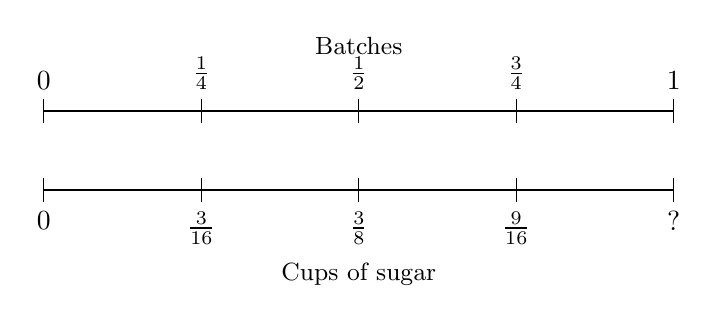
\begin{tikzpicture}[scale=1]
  \draw[thick] (0,0.5) -- (8,0.5);
  \draw[thick] (0,-0.5) -- (8,-0.5);
  \foreach \x/\lab in {0/0, 2/\frac{1}{4}, 4/\frac{1}{2}, 6/\frac{3}{4}, 8/1}
    \draw (\x,0.35) -- (\x,0.65) node[above]{$\lab$};
  \node[above] at (4,1.1) {\small Batches};
  \foreach \x/\lab in {0/0, 2/\frac{3}{16}, 4/\frac{3}{8}, 6/\frac{9}{16}, 8/?}
    \draw (\x,-0.35) -- (\x,-0.65) node[below]{$\lab$};
  \node[below] at (4,-1.3) {\small Cups of sugar};
\end{tikzpicture}
\end{center}

How many cups of sugar are needed for $1$ full batch of cookies?
\end{questionText}
\correctAnswer{$\frac{3}{4}$}
\explanation{From the double number line, $\frac{1}{4}$ batch uses $\frac{3}{16}$ cup. Find the unit rate: $\frac{3}{16} \div \frac{1}{4} = \frac{3}{16} \times 4 = \frac{12}{16} = \frac{3}{4}$ cup per batch.}
\end{practiceQuestion}

\newpage
\section*{1-2-q22 \hfill \normalsize\texttt{tests\_questions\_bank\_2/topics/ch01-02-recognizing-proportional-relationships.tex}}
\begin{practiceQuestion}{1-2-q22}{gmc}
\begin{questionText}
Look at the graph below. Does it represent a proportional relationship?

\begin{center}
\begin{tikzpicture}[scale=0.65]
  \draw[step=1,gray!20,thin] (0,0) grid (7,7);
  \draw[thick,->] (0,0) -- (7.5,0) node[right]{$x$};
  \draw[thick,->] (0,0) -- (0,7.5) node[above]{$y$};
  \foreach \x in {1,...,7} \draw (\x,0.1) -- (\x,-0.1) node[below]{\tiny \x};
  \foreach \y in {1,...,7} \draw (0.1,\y) -- (-0.1,\y) node[left]{\tiny \y};
  \draw[thick,funBlue] (0,2) -- (6,6);
  \fill[funBlue] (0,2) circle (3pt);
  \fill[funBlue] (3,4) circle (3pt);
  \fill[funBlue] (6,6) circle (3pt);
\end{tikzpicture}
\end{center}
\end{questionText}
\choiceA{Yes, because it is a straight line.}
\choiceB{Yes, because the points go up at a constant rate.}
\choiceC{No, because the line does not pass through the origin.}
\choiceD{No, because the slope is less than $1$.}
\correctAnswer{C}
\explanation{A proportional relationship must be a straight line that passes through the origin $(0, 0)$. This line crosses the $y$-axis at $(0, 2)$, so it is not proportional.}
\end{practiceQuestion}

\newpage
\section*{1-2-q24 \hfill \normalsize\texttt{tests\_questions\_bank\_2/topics/ch01-02-recognizing-proportional-relationships.tex}}
\begin{practiceQuestion}{1-2-q24}{gmc}
\begin{questionText}
Two lines are graphed on the same coordinate plane. Line $A$ passes through $(0, 0)$ and $(5, 15)$. Line $B$ passes through $(0, 4)$ and $(5, 19)$.

\begin{center}
\begin{tikzpicture}[scale=0.32]
  \draw[step=2,gray!20,thin] (0,0) grid (10,20);
  \draw[thick,->] (0,0) -- (10.5,0) node[right]{$x$};
  \draw[thick,->] (0,0) -- (0,21) node[above]{$y$};
  \foreach \x in {2,4,6,8,10} \draw (\x,0.2) -- (\x,-0.2) node[below]{\tiny \x};
  \foreach \y in {4,8,12,16,20} \draw (0.2,\y) -- (-0.2,\y) node[left]{\tiny \y};
  \draw[thick,funBlue] (0,0) -- (7,21);
  \draw[thick,funRed] (0,4) -- (6,22);
  \node[right,funBlue] at (6,18) {\small $A$};
  \node[right,funRed] at (5.5,20.5) {\small $B$};
\end{tikzpicture}
\end{center}

Which line represents a proportional relationship?
\end{questionText}
\choiceA{Only Line $A$}
\choiceB{Only Line $B$}
\choiceC{Both lines}
\choiceD{Neither line}
\correctAnswer{A}
\explanation{Line $A$ passes through the origin $(0, 0)$ and is straight, so it is proportional. Line $B$ passes through $(0, 4)$, which means it has a $y$-intercept of $4$ and is not proportional.}
\end{practiceQuestion}

\newpage
\section*{1-2-q26 \hfill \normalsize\texttt{tests\_questions\_bank\_2/topics/ch01-02-recognizing-proportional-relationships.tex}}
\begin{practiceQuestion}{1-2-q26}{gsa}
\begin{questionText}
The scatter plot below shows the heights of plants (in cm) after different numbers of weeks.

\begin{center}
\begin{tikzpicture}[scale=0.55]
  \draw[step=1,gray!20,thin] (0,0) grid (8,10);
  \draw[thick,->] (0,0) -- (8.5,0) node[right]{\small Weeks};
  \draw[thick,->] (0,0) -- (0,10.5) node[above]{\small Height (cm)};
  \foreach \x in {1,...,8} \draw (\x,0.1) -- (\x,-0.1) node[below]{\tiny \x};
  \foreach \y in {1,...,10} \draw (0.1,\y) -- (-0.1,\y) node[left]{\tiny \y};
  \fill[funGreen] (0,0) circle (4pt);
  \fill[funGreen] (2,3) circle (4pt);
  \fill[funGreen] (4,6) circle (4pt);
  \fill[funGreen] (6,9) circle (4pt);
\end{tikzpicture}
\end{center}

Is this a proportional relationship? If yes, what is the growth rate per week?
\end{questionText}
\correctAnswer{$1.5$ cm per week}
\explanation{The points $(0,0)$, $(2,3)$, $(4,6)$, and $(6,9)$ lie on a straight line through the origin. The ratio $\frac{y}{x}$ is $\frac{3}{2} = 1.5$ for every point. The relationship is proportional at $1.5$ cm per week.}
\end{practiceQuestion}

\newpage
\section*{1-2-q27 \hfill \normalsize\texttt{tests\_questions\_bank\_2/topics/ch01-02-recognizing-proportional-relationships.tex}}
\begin{practiceQuestion}{1-2-q27}{gsa}
\begin{questionText}
The graph below shows the cost of renting kayaks.

\begin{center}
\begin{tikzpicture}[scale=0.5]
  \draw[step=1,gray!20,thin] (0,0) grid (8,10);
  \draw[thick,->] (0,0) -- (8.5,0) node[right]{\small Hours};
  \draw[thick,->] (0,0) -- (0,10.5) node[above]{\small Cost (\$)};
  \foreach \x in {1,...,8} \draw (\x,0.1) -- (\x,-0.1) node[below]{\tiny \x};
  \foreach \y in {2,4,...,10} \draw (0.1,\y) -- (-0.1,\y) node[left]{\tiny \y0};
  \fill[funPurple] (0,2) circle (4pt);
  \fill[funPurple] (1,3.5) circle (4pt);
  \fill[funPurple] (2,5) circle (4pt);
  \fill[funPurple] (4,8) circle (4pt);
  \draw[thick,funPurple] (0,2) -- (4,8);
\end{tikzpicture}
\end{center}

The $y$-axis values are in tens of dollars ($20, 40, \ldots$). Why is this relationship \textbf{not} proportional? State the reason.
\end{questionText}
\correctAnswer{The line does not pass through the origin}
\explanation{The graph starts at $(0, 20)$, meaning there is a $\$20$ base fee even for $0$ hours. A proportional relationship must pass through $(0, 0)$. Since the line starts above the origin, the relationship is not proportional.}
\end{practiceQuestion}

\newpage
\section*{1-3-q22 \hfill \normalsize\texttt{tests\_questions\_bank\_2/topics/ch01-03-finding-the-constant-of-proportionality.tex}}
\begin{practiceQuestion}{1-3-q22}{gmc}
\begin{questionText}
The graph below shows a proportional relationship. What is the constant of proportionality?

\begin{center}
\begin{tikzpicture}[scale=0.55]
  \draw[step=1,gray!20,thin] (0,0) grid (8,8);
  \draw[thick,->] (0,0) -- (8.5,0) node[right]{$x$};
  \draw[thick,->] (0,0) -- (0,8.5) node[above]{$y$};
  \foreach \x in {1,...,8} \draw (\x,0.1) -- (\x,-0.1) node[below]{\tiny \x};
  \foreach \y in {1,...,8} \draw (0.1,\y) -- (-0.1,\y) node[left]{\tiny \y};
  \draw[thick,funBlue] (0,0) -- (8,6);
  \fill[funBlue] (0,0) circle (3pt);
  \fill[funBlue] (4,3) circle (3pt);
  \fill[funBlue] (8,6) circle (3pt);
\end{tikzpicture}
\end{center}
\end{questionText}
\choiceA{$k = \frac{4}{3}$}
\choiceB{$k = \frac{3}{4}$}
\choiceC{$k = 3$}
\choiceD{$k = 4$}
\correctAnswer{B}
\explanation{Read the point $(4, 3)$ from the graph. The constant of proportionality is $k = \frac{y}{x} = \frac{3}{4}$. Check with $(8,6)$: $\frac{6}{8} = \frac{3}{4}$ \checkmark.}
\end{practiceQuestion}

\newpage
\section*{1-3-q24 \hfill \normalsize\texttt{tests\_questions\_bank\_2/topics/ch01-03-finding-the-constant-of-proportionality.tex}}
\begin{practiceQuestion}{1-3-q24}{gmc}
\begin{questionText}
Two proportional lines are graphed on the same axes. Line $P$ passes through $(3, 6)$ and Line $Q$ passes through $(3, 9)$. Both pass through the origin.

\begin{center}
\begin{tikzpicture}[scale=0.45]
  \draw[step=1,gray!20,thin] (0,0) grid (6,12);
  \draw[thick,->] (0,0) -- (6.5,0) node[right]{$x$};
  \draw[thick,->] (0,0) -- (0,12.5) node[above]{$y$};
  \foreach \x in {1,...,6} \draw (\x,0.1) -- (\x,-0.1) node[below]{\tiny \x};
  \foreach \y in {2,4,...,12} \draw (0.1,\y) -- (-0.1,\y) node[left]{\tiny \y};
  \draw[thick,funBlue] (0,0) -- (6,12);
  \draw[thick,funOrange] (0,0) -- (6,12);
  \draw[thick,funBlue] (0,0) -- (5,10);
  \draw[thick,funOrange] (0,0) -- (4,12);
  \fill[funBlue] (3,6) circle (3pt) node[right]{\tiny $P$};
  \fill[funOrange] (3,9) circle (3pt) node[left]{\tiny $Q$};
\end{tikzpicture}
\end{center}

How much greater is $k_Q$ than $k_P$?
\end{questionText}
\choiceA{$1$}
\choiceB{$3$}
\choiceC{$\frac{1}{3}$}
\choiceD{$\frac{3}{2}$}
\correctAnswer{A}
\explanation{$k_P = \frac{6}{3} = 2$ and $k_Q = \frac{9}{3} = 3$. The difference is $3 - 2 = 1$.}
\end{practiceQuestion}

\newpage
\section*{1-3-q25 \hfill \normalsize\texttt{tests\_questions\_bank\_2/topics/ch01-03-finding-the-constant-of-proportionality.tex}}
\begin{practiceQuestion}{1-3-q25}{gsa}
\begin{questionText}
The graph below shows the cost of renting roller skates per hour.

\begin{center}
\begin{tikzpicture}[scale=0.5]
  \draw[step=1,gray!20,thin] (0,0) grid (8,10);
  \draw[thick,->] (0,0) -- (8.5,0) node[right]{\small Hours};
  \draw[thick,->] (0,0) -- (0,10.5) node[above]{\small Cost (\$)};
  \foreach \x in {1,...,8} \draw (\x,0.1) -- (\x,-0.1) node[below]{\tiny \x};
  \foreach \y in {1,...,10} \draw (0.1,\y) -- (-0.1,\y) node[left]{\tiny \y};
  \draw[thick,funGreen] (0,0) -- (8,10);
  \fill[funGreen] (0,0) circle (3pt);
  \fill[funGreen] (2,2.5) circle (3pt);
  \fill[funGreen] (4,5) circle (3pt);
  \fill[funGreen] (8,10) circle (3pt);
\end{tikzpicture}
\end{center}

What is the constant of proportionality? Include units.
\end{questionText}
\correctAnswer{$\$1.25$ per hour}
\explanation{Use the point $(4, 5)$: $k = \frac{5}{4} = 1.25$ dollars per hour. Check: $\frac{2.5}{2} = 1.25$ and $\frac{10}{8} = 1.25$ \checkmark.}
\end{practiceQuestion}

\newpage
\section*{1-3-q26 \hfill \normalsize\texttt{tests\_questions\_bank\_2/topics/ch01-03-finding-the-constant-of-proportionality.tex}}
\begin{practiceQuestion}{1-3-q26}{gsa}
\begin{questionText}
The double number line below shows a proportional relationship between feet and seconds.

\begin{center}
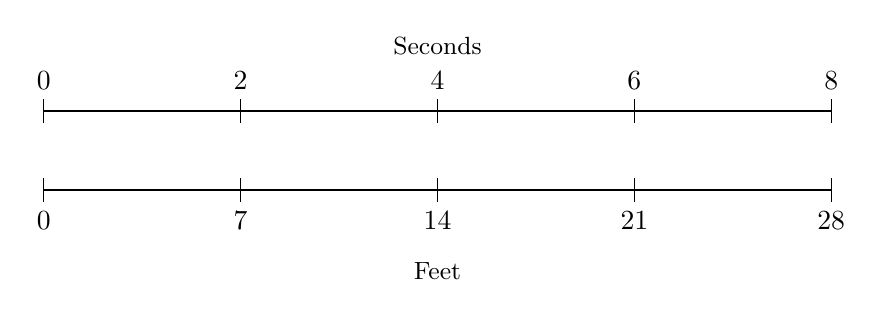
\begin{tikzpicture}[scale=1]
  \draw[thick] (0,0.5) -- (10,0.5);
  \draw[thick] (0,-0.5) -- (10,-0.5);
  \foreach \x/\lab in {0/0, 2.5/2, 5/4, 7.5/6, 10/8}
    \draw (\x,0.35) -- (\x,0.65) node[above]{$\lab$};
  \node[above] at (5,1.1) {\small Seconds};
  \foreach \x/\lab in {0/0, 2.5/7, 5/14, 7.5/21, 10/28}
    \draw (\x,-0.35) -- (\x,-0.65) node[below]{$\lab$};
  \node[below] at (5,-1.3) {\small Feet};
\end{tikzpicture}
\end{center}

What is the constant of proportionality in feet per second?
\end{questionText}
\correctAnswer{$3.5$}
\explanation{Divide feet by seconds from any pair: $\frac{7}{2} = 3.5$, $\frac{14}{4} = 3.5$, $\frac{21}{6} = 3.5$, $\frac{28}{8} = 3.5$. The constant is $3.5$ feet per second.}
\end{practiceQuestion}

\newpage
\section*{1-4-q22 \hfill \normalsize\texttt{tests\_questions\_bank\_2/topics/ch01-04-writing-equations-for-proportional-relationships.tex}}
\begin{practiceQuestion}{1-4-q22}{gmc}
\begin{questionText}
The graph below shows a proportional relationship between hours worked and money earned.

\begin{center}
\begin{tikzpicture}[scale=0.5]
  \draw[step=1,gray!20,thin] (0,0) grid (8,10);
  \draw[thick,->] (0,0) -- (8.5,0) node[right]{\small Hours};
  \draw[thick,->] (0,0) -- (0,10.5) node[above]{\small Earnings (\$)};
  \foreach \x in {1,...,8} \draw (\x,0.1) -- (\x,-0.1) node[below]{\tiny \x};
  \foreach \y in {1,...,10} \draw (0.1,\y) -- (-0.1,\y) node[left]{\tiny \y};
  \draw[thick,funBlue] (0,0) -- (8,10);
  \fill[funBlue] (0,0) circle (3pt);
  \fill[funBlue] (4,5) circle (3pt);
  \fill[funBlue] (8,10) circle (3pt);
\end{tikzpicture}
\end{center}

Which equation represents this graph?
\end{questionText}
\choiceA{$e = 0.8h$}
\choiceB{$e = 1.25h$}
\choiceC{$e = 5h$}
\choiceD{$e = 2h$}
\correctAnswer{B}
\explanation{From the graph, the point $(4, 5)$ gives $k = \frac{5}{4} = 1.25$. The equation is $e = 1.25h$.}
\end{practiceQuestion}

\newpage
\section*{1-4-q24 \hfill \normalsize\texttt{tests\_questions\_bank\_2/topics/ch01-04-writing-equations-for-proportional-relationships.tex}}
\begin{practiceQuestion}{1-4-q24}{gmc}
\begin{questionText}
The double number line below shows the proportional relationship between liters of paint and square meters covered.

\begin{center}
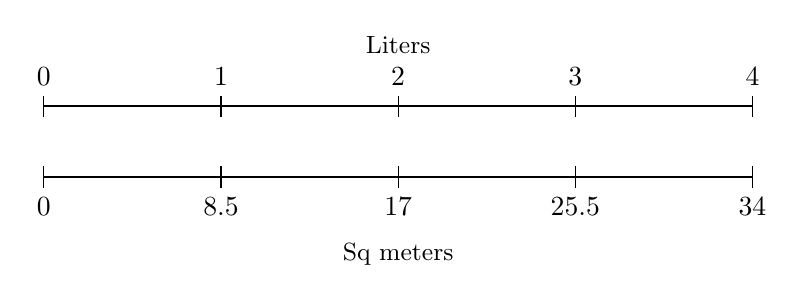
\begin{tikzpicture}[scale=0.9]
  \draw[thick] (0,0.5) -- (10,0.5);
  \draw[thick] (0,-0.5) -- (10,-0.5);
  \foreach \x/\lab in {0/0, 2.5/1, 5/2, 7.5/3, 10/4}
    \draw (\x,0.35) -- (\x,0.65) node[above]{$\lab$};
  \node[above] at (5,1.1) {\small Liters};
  \foreach \x/\lab in {0/0, 2.5/8.5, 5/17, 7.5/25.5, 10/34}
    \draw (\x,-0.35) -- (\x,-0.65) node[below]{$\lab$};
  \node[below] at (5,-1.3) {\small Sq meters};
\end{tikzpicture}
\end{center}

Which equation represents the relationship?
\end{questionText}
\choiceA{$s = 8.5l$}
\choiceB{$l = 8.5s$}
\choiceC{$s = l + 8.5$}
\choiceD{$s = 4.25l$}
\correctAnswer{A}
\explanation{From the double number line, $1$ liter covers $8.5$ sq meters. The equation is $s = 8.5l$. Check: $2$ liters covers $8.5 \times 2 = 17$ \checkmark.}
\end{practiceQuestion}

\newpage
\section*{1-4-q25 \hfill \normalsize\texttt{tests\_questions\_bank\_2/topics/ch01-04-writing-equations-for-proportional-relationships.tex}}
\begin{practiceQuestion}{1-4-q25}{gsa}
\begin{questionText}
The graph below shows a proportional relationship.

\begin{center}
\begin{tikzpicture}[scale=0.5]
  \draw[step=1,gray!20,thin] (0,0) grid (10,8);
  \draw[thick,->] (0,0) -- (10.5,0) node[right]{$x$};
  \draw[thick,->] (0,0) -- (0,8.5) node[above]{$y$};
  \foreach \x in {2,4,...,10} \draw (\x,0.1) -- (\x,-0.1) node[below]{\tiny \x};
  \foreach \y in {1,...,8} \draw (0.1,\y) -- (-0.1,\y) node[left]{\tiny \y};
  \draw[thick,funOrange] (0,0) -- (10,6);
  \fill[funOrange] (0,0) circle (3pt);
  \fill[funOrange] (5,3) circle (3pt);
  \fill[funOrange] (10,6) circle (3pt);
\end{tikzpicture}
\end{center}

Write the equation for this proportional relationship.
\end{questionText}
\correctAnswer{$y = 0.6x$}
\explanation{From the graph, the point $(5, 3)$ gives $k = \frac{3}{5} = 0.6$. The equation is $y = 0.6x$. Check: $0.6 \times 10 = 6$ \checkmark.}
\end{practiceQuestion}

\newpage
\section*{1-4-q27 \hfill \normalsize\texttt{tests\_questions\_bank\_2/topics/ch01-04-writing-equations-for-proportional-relationships.tex}}
\begin{practiceQuestion}{1-4-q27}{gsa}
\begin{questionText}
A proportional graph passes through the points shown below.

\begin{center}
\begin{tikzpicture}[scale=0.45]
  \draw[step=1,gray!20,thin] (0,0) grid (10,10);
  \draw[thick,->] (0,0) -- (10.5,0) node[right]{$x$};
  \draw[thick,->] (0,0) -- (0,10.5) node[above]{$y$};
  \foreach \x in {1,...,10} \draw (\x,0.1) -- (\x,-0.1) node[below]{\tiny \x};
  \foreach \y in {1,...,10} \draw (0.1,\y) -- (-0.1,\y) node[left]{\tiny \y};
  \draw[thick,funPurple] (0,0) -- (10,7.5);
  \fill[funPurple] (0,0) circle (3pt);
  \fill[funPurple] (4,3) circle (3pt);
  \fill[funPurple] (8,6) circle (3pt);
\end{tikzpicture}
\end{center}

Write the equation, and find the value of $y$ when $x = 14$.
\end{questionText}
\correctAnswer{$10.5$}
\explanation{From the point $(4, 3)$: $k = \frac{3}{4} = 0.75$. The equation is $y = 0.75x$. Substitute $x = 14$: $y = 0.75 \times 14 = 10.5$.}
\end{practiceQuestion}

\newpage
\section*{1-5-q22 \hfill \normalsize\texttt{tests\_questions\_bank\_2/topics/ch01-05-graphing-proportional-relationships.tex}}
\begin{practiceQuestion}{1-5-q22}{gmc}
\begin{questionText}
The graph below shows the distance a train travels over time.

\begin{center}
\begin{tikzpicture}[scale=0.5]
  \draw[step=1,gray!20,thin] (0,0) grid (8,10);
  \draw[thick,->] (0,0) -- (8.5,0) node[right]{\small Hours};
  \draw[thick,->] (0,0) -- (0,10.5) node[above]{\small Distance (mi)};
  \foreach \x in {1,...,8} \draw (\x,0.1) -- (\x,-0.1) node[below]{\tiny \x};
  \foreach \y/\lab in {1/50,2/100,3/150,4/200,5/250,6/300,7/350,8/400,9/450,10/500}
    \draw (0.1,\y) -- (-0.1,\y) node[left]{\tiny \lab};
  \draw[thick,funBlue] (0,0) -- (8,6.4);
  \fill[funBlue] (0,0) circle (3pt);
  \fill[funBlue] (1,0.8) circle (3pt);
  \fill[funBlue] (5,4) circle (3pt);
\end{tikzpicture}
\end{center}

What is the train's speed in miles per hour?
\end{questionText}
\choiceA{$40$ mph}
\choiceB{$50$ mph}
\choiceC{$80$ mph}
\choiceD{$100$ mph}
\correctAnswer{A}
\explanation{From the point $(1, 0.8)$ on the graph, and since each grid unit on the $y$-axis equals $50$ miles, the $y$-value at $x = 1$ is $0.8 \times 50 = 40$ miles. The unit rate from the point $(5, 200)$ confirms: $200 \div 5 = 40$ mph.}
\end{practiceQuestion}

\newpage
\section*{1-5-q23 \hfill \normalsize\texttt{tests\_questions\_bank\_2/topics/ch01-05-graphing-proportional-relationships.tex}}
\begin{practiceQuestion}{1-5-q23}{gmc}
\begin{questionText}
Two proportional lines are graphed below. Line $A$ (blue) passes through $(4, 6)$. Line $B$ (orange) passes through $(4, 10)$.

\begin{center}
\begin{tikzpicture}[scale=0.5]
  \draw[step=1,gray!20,thin] (0,0) grid (8,12);
  \draw[thick,->] (0,0) -- (8.5,0) node[right]{$x$};
  \draw[thick,->] (0,0) -- (0,12.5) node[above]{$y$};
  \foreach \x in {1,...,8} \draw (\x,0.1) -- (\x,-0.1) node[below]{\tiny \x};
  \foreach \y in {2,4,...,12} \draw (0.1,\y) -- (-0.1,\y) node[left]{\tiny \y};
  \draw[thick,funBlue] (0,0) -- (8,12);
  \draw[thick,funOrange] (0,0) -- (5,12.5);
  \fill[funBlue] (4,6) circle (3pt) node[right=2pt]{\tiny $A$};
  \fill[funOrange] (4,10) circle (3pt) node[left=2pt]{\tiny $B$};
\end{tikzpicture}
\end{center}

What is the unit rate of Line $B$?
\end{questionText}
\choiceA{$1.5$}
\choiceB{$2$}
\choiceC{$2.5$}
\choiceD{$4$}
\correctAnswer{C}
\explanation{Line $B$ passes through $(4, 10)$ and the origin: $k = \frac{10}{4} = 2.5$. The unit rate is $2.5$.}
\end{practiceQuestion}

\newpage
\section*{1-5-q24 \hfill \normalsize\texttt{tests\_questions\_bank\_2/topics/ch01-05-graphing-proportional-relationships.tex}}
\begin{practiceQuestion}{1-5-q24}{gmc}
\begin{questionText}
The graph below represents a proportional relationship between cups of flour and number of cakes baked.

\begin{center}
\begin{tikzpicture}[scale=0.5]
  \draw[step=1,gray!20,thin] (0,0) grid (10,8);
  \draw[thick,->] (0,0) -- (10.5,0) node[right]{\small Cakes};
  \draw[thick,->] (0,0) -- (0,8.5) node[above]{\small Cups of flour};
  \foreach \x in {1,...,10} \draw (\x,0.1) -- (\x,-0.1) node[below]{\tiny \x};
  \foreach \y in {1,...,8} \draw (0.1,\y) -- (-0.1,\y) node[left]{\tiny \y};
  \draw[thick,funGreen] (0,0) -- (10,7.5);
  \fill[funGreen] (0,0) circle (3pt);
  \fill[funGreen] (4,3) circle (3pt);
  \fill[funGreen] (8,6) circle (3pt);
\end{tikzpicture}
\end{center}

How many cups of flour are needed for $12$ cakes?
\end{questionText}
\choiceA{$6$}
\choiceB{$8$}
\choiceC{$9$}
\choiceD{$12$}
\correctAnswer{C}
\explanation{From the point $(4, 3)$: $k = \frac{3}{4} = 0.75$ cups per cake. For $12$ cakes: $0.75 \times 12 = 9$ cups.}
\end{practiceQuestion}

\newpage
\section*{1-5-q25 \hfill \normalsize\texttt{tests\_questions\_bank\_2/topics/ch01-05-graphing-proportional-relationships.tex}}
\begin{practiceQuestion}{1-5-q25}{gsa}
\begin{questionText}
The graph below shows two proportional lines.

\begin{center}
\begin{tikzpicture}[scale=0.5]
  \draw[step=1,gray!20,thin] (0,0) grid (8,10);
  \draw[thick,->] (0,0) -- (8.5,0) node[right]{$x$};
  \draw[thick,->] (0,0) -- (0,10.5) node[above]{$y$};
  \foreach \x in {1,...,8} \draw (\x,0.1) -- (\x,-0.1) node[below]{\tiny \x};
  \foreach \y in {1,...,10} \draw (0.1,\y) -- (-0.1,\y) node[left]{\tiny \y};
  \draw[thick,funBlue] (0,0) -- (8,8);
  \draw[thick,funRed] (0,0) -- (5,10);
  \fill[funBlue] (4,4) circle (3pt) node[below right]{\tiny $A(4,4)$};
  \fill[funRed] (5,10) circle (3pt) node[left]{\tiny $B(5,10)$};
\end{tikzpicture}
\end{center}

What is the difference in the unit rates of Line $B$ and Line $A$?
\end{questionText}
\correctAnswer{$1$}
\explanation{Line $A$: $k = \frac{4}{4} = 1$. Line $B$: $k = \frac{10}{5} = 2$. Difference: $2 - 1 = 1$.}
\end{practiceQuestion}

\newpage
\section*{1-5-q26 \hfill \normalsize\texttt{tests\_questions\_bank\_2/topics/ch01-05-graphing-proportional-relationships.tex}}
\begin{practiceQuestion}{1-5-q26}{gsa}
\begin{questionText}
The coordinate plane below shows a proportional relationship between time (seconds) and distance (meters).

\begin{center}
\begin{tikzpicture}[scale=0.55]
  \draw[step=1,gray!20,thin] (0,0) grid (8,10);
  \draw[thick,->] (0,0) -- (8.5,0) node[right]{\small Seconds};
  \draw[thick,->] (0,0) -- (0,10.5) node[above]{\small Meters};
  \foreach \x in {1,...,8} \draw (\x,0.1) -- (\x,-0.1) node[below]{\tiny \x};
  \foreach \y in {1,...,10} \draw (0.1,\y) -- (-0.1,\y) node[left]{\tiny \y};
  \draw[thick,funOrange] (0,0) -- (8,7);
  \fill[funOrange] (0,0) circle (3pt);
  \fill[funOrange] (4,3.5) circle (3pt);
  \fill[funOrange] (8,7) circle (3pt);
\end{tikzpicture}
\end{center}

What is the speed in meters per second? How far does the object travel in $12$ seconds?
\end{questionText}
\correctAnswer{$10.5$ meters}
\explanation{From $(8, 7)$: $k = \frac{7}{8} = 0.875$ m/s. For $12$ seconds: $0.875 \times 12 = 10.5$ meters.}
\end{practiceQuestion}

\newpage
\section*{1-5-q27 \hfill \normalsize\texttt{tests\_questions\_bank\_2/topics/ch01-05-graphing-proportional-relationships.tex}}
\begin{practiceQuestion}{1-5-q27}{gsa}
\begin{questionText}
The graph below shows two workers' earnings over time. Both pass through the origin.

\begin{center}
\begin{tikzpicture}[scale=0.5]
  \draw[step=1,gray!20,thin] (0,0) grid (8,10);
  \draw[thick,->] (0,0) -- (8.5,0) node[right]{\small Hours};
  \draw[thick,->] (0,0) -- (0,10.5) node[above]{\small Earnings (\$)};
  \foreach \x in {1,...,8} \draw (\x,0.1) -- (\x,-0.1) node[below]{\tiny \x};
  \foreach \y/\lab in {2/20,4/40,6/60,8/80,10/100}
    \draw (0.1,\y) -- (-0.1,\y) node[left]{\tiny \lab};
  \draw[thick,funBlue] (0,0) -- (8,9.6);
  \draw[thick,funRed] (0,0) -- (8,6.4);
  \fill[funBlue] (5,6) circle (3pt) node[above left]{\tiny Worker $A$};
  \fill[funRed] (5,4) circle (3pt) node[below right]{\tiny Worker $B$};
\end{tikzpicture}
\end{center}

Each $y$-axis unit equals $\$10$. How much more does Worker $A$ earn than Worker $B$ in an $8$-hour shift?
\end{questionText}
\correctAnswer{$\$32$}
\explanation{Each $y$-unit is $\$10$, so Worker $A$ at $(5, 6)$ earns $\$60$ in $5$ hours ($\$12$/hr) and Worker $B$ at $(5, 4)$ earns $\$40$ in $5$ hours ($\$8$/hr). In $8$ hours: $A$ earns $12 \times 8 = \$96$ and $B$ earns $8 \times 8 = \$64$. Difference: $96 - 64 = \$32$.}
\end{practiceQuestion}

\newpage
\section*{1-6-q23 \hfill \normalsize\texttt{tests\_questions\_bank\_2/topics/ch01-06-applying-proportional-reasoning.tex}}
\begin{practiceQuestion}{1-6-q23}{gmc}
\begin{questionText}
The bar graph below shows the cost per pound of two different cheeses.

\begin{center}
\begin{tikzpicture}[scale=0.7]
  \draw[thick,->] (0,0) -- (0,5) node[above]{\small \$/lb};
  \draw[thick,->] (0,0) -- (5.5,0);
  \fill[funBlue] (0.5,0) rectangle (2,3.6);
  \fill[funOrange] (2.5,0) rectangle (4,4.5);
  \node[below] at (1.25,-0.1) {\small Cheddar};
  \node[below] at (3.25,-0.1) {\small Swiss};
  \foreach \y/\lab in {1/\$2,2/\$4,3/\$6,4/\$8}
    \draw (-0.1,\y) -- (0.1,\y) node[left=4pt]{\small \lab};
\end{tikzpicture}
\end{center}

Marco buys $3$ pounds of cheddar and $2$ pounds of Swiss. Each bar unit equals $\$2$. What is the total cost?
\end{questionText}
\choiceA{$\$28.80$}
\choiceB{$\$30.60$}
\choiceC{$\$36.00$}
\choiceD{$\$39.60$}
\correctAnswer{D}
\explanation{Each grid unit on the y-axis is $\$2$. Cheddar bar reaches $3.6$ units $= 3.6 \times 2 = \$7.20$/lb. Swiss bar reaches $4.5$ units $= 4.5 \times 2 = \$9.00$/lb. Cheddar: $7.20 \times 3 = \$21.60$. Swiss: $9.00 \times 2 = \$18.00$. Total: $21.60 + 18.00 = \$39.60$.}
\end{practiceQuestion}

\newpage
\section*{1-6-q24 \hfill \normalsize\texttt{tests\_questions\_bank\_2/topics/ch01-06-applying-proportional-reasoning.tex}}
\begin{practiceQuestion}{1-6-q24}{gmc}
\begin{questionText}
A map uses the scale shown below.

\begin{center}
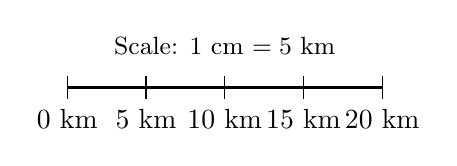
\begin{tikzpicture}
  \draw[thick] (0,0) -- (4,0);
  \foreach \x/\lab in {0/0,1/5,2/10,3/15,4/20}
    \draw (\x,0.15) -- (\x,-0.15) node[below]{$\lab$ km};
  \node[above] at (2,0.3) {\small Scale: $1$ cm $= 5$ km};
\end{tikzpicture}
\end{center}

On the map, a road is $7.4$ cm long. What is the actual distance?
\end{questionText}
\choiceA{$12.4$ km}
\choiceB{$37$ km}
\choiceC{$42$ km}
\choiceD{$74$ km}
\correctAnswer{B}
\explanation{Each centimeter on the map equals $5$ km. Multiply: $7.4 \times 5 = 37$ km.}
\end{practiceQuestion}

\newpage
\section*{1-6-q26 \hfill \normalsize\texttt{tests\_questions\_bank\_2/topics/ch01-06-applying-proportional-reasoning.tex}}
\begin{practiceQuestion}{1-6-q26}{gsa}
\begin{questionText}
The double number line shows the relationship between ounces of dog food and the number of dogs fed.

\begin{center}
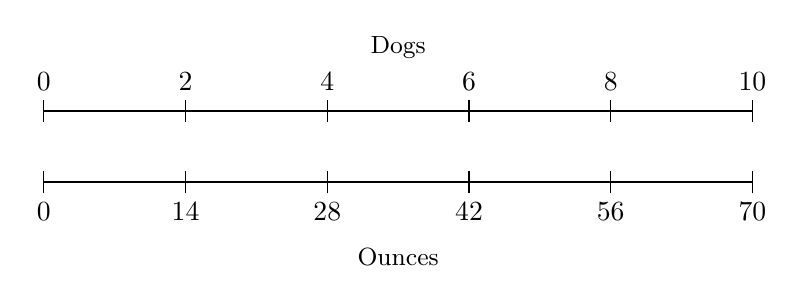
\begin{tikzpicture}[scale=0.9]
  \draw[thick] (0,0.5) -- (10,0.5);
  \draw[thick] (0,-0.5) -- (10,-0.5);
  \foreach \x/\lab in {0/0, 2/2, 4/4, 6/6, 8/8, 10/10}
    \draw (\x,0.35) -- (\x,0.65) node[above]{$\lab$};
  \node[above] at (5,1.1) {\small Dogs};
  \foreach \x/\lab in {0/0, 2/14, 4/28, 6/42, 8/56, 10/70}
    \draw (\x,-0.35) -- (\x,-0.65) node[below]{$\lab$};
  \node[below] at (5,-1.3) {\small Ounces};
\end{tikzpicture}
\end{center}

How many ounces of dog food are needed for $15$ dogs?
\end{questionText}
\correctAnswer{$105$}
\explanation{From the double number line, each dog needs $\frac{14}{2} = 7$ ounces. For $15$ dogs: $7 \times 15 = 105$ ounces.}
\end{practiceQuestion}

\newpage
\section*{1-6-q27 \hfill \normalsize\texttt{tests\_questions\_bank\_2/topics/ch01-06-applying-proportional-reasoning.tex}}
\begin{practiceQuestion}{1-6-q27}{gsa}
\begin{questionText}
The graph below shows the proportional relationship between hours and the number of bracelets a crafter makes.

\begin{center}
\begin{tikzpicture}[scale=0.5]
  \draw[step=1,gray!20,thin] (0,0) grid (8,10);
  \draw[thick,->] (0,0) -- (8.5,0) node[right]{\small Hours};
  \draw[thick,->] (0,0) -- (0,10.5) node[above]{\small Bracelets};
  \foreach \x in {1,...,8} \draw (\x,0.1) -- (\x,-0.1) node[below]{\tiny \x};
  \foreach \y in {1,...,10} \draw (0.1,\y) -- (-0.1,\y) node[left]{\tiny \y};
  \draw[thick,funPurple] (0,0) -- (8,6);
  \fill[funPurple] (0,0) circle (3pt);
  \fill[funPurple] (4,3) circle (3pt);
  \fill[funPurple] (8,6) circle (3pt);
\end{tikzpicture}
\end{center}

How many bracelets can the crafter make in a $10$-hour day?
\end{questionText}
\correctAnswer{$7.5$}
\explanation{From the point $(4, 3)$: $k = \frac{3}{4} = 0.75$ bracelets per hour. For $10$ hours: $0.75 \times 10 = 7.5$ bracelets.}
\end{practiceQuestion}

\newpage
\section*{m-1-6-q23 \hfill \normalsize\texttt{tests\_questions\_bank\_2/topics\_modified/ch01-06-applying-proportional-reasoning.tex}}
\begin{practiceQuestion}{m-1-6-q23}{gmc}
\begin{questionText}
The graph below shows two workers' earnings over time.

\begin{center}
\begin{tikzpicture}[scale=0.5]
  \draw[step=1,gray!20,thin] (0,0) grid (10,10);
  \draw[thick,->] (0,0) -- (10.5,0) node[right]{\small Hours};
  \draw[thick,->] (0,0) -- (0,10.5) node[above]{\small Earnings (\$)};
  \foreach \x in {1,...,10} \draw (\x,0.1) -- (\x,-0.1) node[below]{\tiny \x};
  \foreach \y/\lab in {2/20,4/40,6/60,8/80,10/100}
    \draw (0.1,\y) -- (-0.1,\y) node[left]{\tiny \lab};
  \draw[thick,funBlue] (0,0) -- (10,9);
  \draw[thick,funRed] (0,0) -- (10,6);
  \fill[funBlue] (0,0) circle (3pt); \fill[funBlue] (10,9) circle (3pt);
  \fill[funRed] (0,0) circle (3pt); \fill[funRed] (10,6) circle (3pt);
  \node[funBlue,right] at (10,9) {\tiny Worker A};
  \node[funRed,right] at (10,6) {\tiny Worker B};
\end{tikzpicture}
\end{center}

Each y-axis unit $= \$10$. Which is the best estimate of the combined earnings after $6$ hours?
\end{questionText}
\choiceA{About $\$60$}
\choiceB{About $\$72$}
\choiceC{About $\$90$}
\choiceD{About $\$108$}
\correctAnswer{C}
\explanation{Worker A: slope $= \frac{90}{10} = \$9$/hr. At $6$ hrs: $9 \times 6 = \$54$. Worker B: slope $= \frac{60}{10} = \$6$/hr. At $6$ hrs: $6 \times 6 = \$36$. Combined: $54 + 36 = \$90$.}
\end{practiceQuestion}

\newpage
\section*{m-1-6-q24 \hfill \normalsize\texttt{tests\_questions\_bank\_2/topics\_modified/ch01-06-applying-proportional-reasoning.tex}}
\begin{practiceQuestion}{m-1-6-q24}{gmc}
\begin{questionText}
A double number line shows the relationship between gallons of paint and square feet of wall covered.

\begin{center}
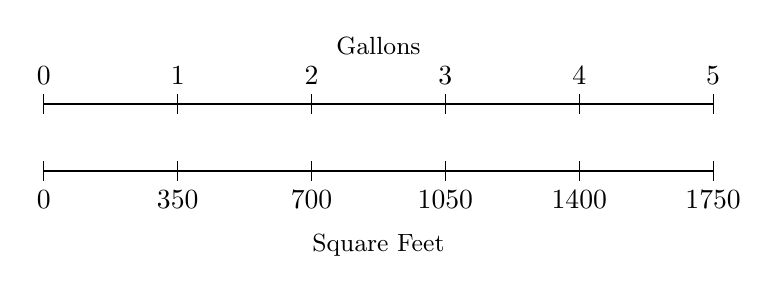
\begin{tikzpicture}[scale=0.85]
  \draw[thick] (0,0.5) -- (10,0.5);
  \draw[thick] (0,-0.5) -- (10,-0.5);
  \foreach \x/\lab in {0/0, 2/1, 4/2, 6/3, 8/4, 10/5}
    \draw (\x,0.35) -- (\x,0.65) node[above]{$\lab$};
  \node[above] at (5,1.1) {\small Gallons};
  \foreach \x/\lab in {0/0, 2/350, 4/700, 6/1050, 8/1400, 10/1750}
    \draw (\x,-0.35) -- (\x,-0.65) node[below]{$\lab$};
  \node[below] at (5,-1.3) {\small Square Feet};
\end{tikzpicture}
\end{center}

A room has $2{,}100$ sq ft of wall. Estimate the number of gallons needed.
\end{questionText}
\choiceA{$5$}
\choiceB{$6$}
\choiceC{$7$}
\choiceD{$8$}
\correctAnswer{B}
\explanation{Rate: $350$ sq ft per gallon. Gallons: $2{,}100 \div 350 = 6$.}
\end{practiceQuestion}

\newpage
\section*{m-1-6-q26 \hfill \normalsize\texttt{tests\_questions\_bank\_2/topics\_modified/ch01-06-applying-proportional-reasoning.tex}}
\begin{practiceQuestion}{m-1-6-q26}{gsa}
\begin{questionText}
The graph below shows two streaming services' monthly data usage.

\begin{center}
\begin{tikzpicture}[scale=0.5]
  \draw[step=1,gray!20,thin] (0,0) grid (8,10);
  \draw[thick,->] (0,0) -- (8.5,0) node[right]{\small Hours};
  \draw[thick,->] (0,0) -- (0,10.5) node[above]{\small GB};
  \foreach \x in {1,...,8} \draw (\x,0.1) -- (\x,-0.1) node[below]{\tiny \x};
  \foreach \y in {2,4,6,8,10} \draw (0.1,\y) -- (-0.1,\y) node[left]{\tiny \y};
  \draw[thick,funGreen] (0,0) -- (8,6);
  \draw[thick,funOrange] (0,0) -- (8,4);
  \fill[funGreen] (4,3) circle (3pt);
  \fill[funOrange] (4,2) circle (3pt);
  \node[funGreen,right] at (8.1,6) {\tiny Service A};
  \node[funOrange,right] at (8.1,4) {\tiny Service B};
\end{tikzpicture}
\end{center}

How many more GB does Service A use than Service B in $12$ hours?
\end{questionText}
\correctAnswer{$3$ GB}
\explanation{Service A: from $(4, 3)$, rate $= \frac{3}{4} = 0.75$ GB/hr. In $12$ hrs: $0.75 \times 12 = 9$ GB. Service B: from $(4, 2)$, rate $= \frac{2}{4} = 0.5$ GB/hr. In $12$ hrs: $0.5 \times 12 = 6$ GB. Difference: $9 - 6 = 3$ GB.}
\end{practiceQuestion}

\newpage
\section*{1-7-q22 \hfill \normalsize\texttt{tests\_questions\_bank\_2/topics\_additional/ch01-07-proportional-reasoning-with-scale-models.tex}}
\begin{practiceQuestion}{1-7-q22}{gmc}
\begin{questionText}
The scale drawing below shows the floor plan of a rectangular room.

\begin{center}
\begin{tikzpicture}[scale=0.9]
  \draw[thick,funBlue,fill=funBlue!10] (0,0) rectangle (5,3);
  \draw[<->,thick] (0,-0.4) -- (5,-0.4) node[midway,below]{\small $10$ cm};
  \draw[<->,thick] (-0.4,0) -- (-0.4,3) node[midway,left]{\small $6$ cm};
  \node at (2.5,1.5) {\small Room};
  \node at (2.5,-1.2) {\small Scale: $1$ cm $= 2$ ft};
\end{tikzpicture}
\end{center}

What is the actual area of the room?
\end{questionText}
\choiceA{$60$ sq ft}
\choiceB{$120$ sq ft}
\choiceC{$200$ sq ft}
\choiceD{$240$ sq ft}
\correctAnswer{D}
\explanation{Actual length $= 10 \times 2 = 20$ ft. Actual width $= 6 \times 2 = 12$ ft. Area $= 20 \times 12 = 240$ sq ft.}
\end{practiceQuestion}

\newpage
\section*{1-7-q23 \hfill \normalsize\texttt{tests\_questions\_bank\_2/topics\_additional/ch01-07-proportional-reasoning-with-scale-models.tex}}
\begin{practiceQuestion}{1-7-q23}{gmc}
\begin{questionText}
The double number line below shows the relationship between model length and actual length for a $1 : 250$ scale model.

\begin{center}
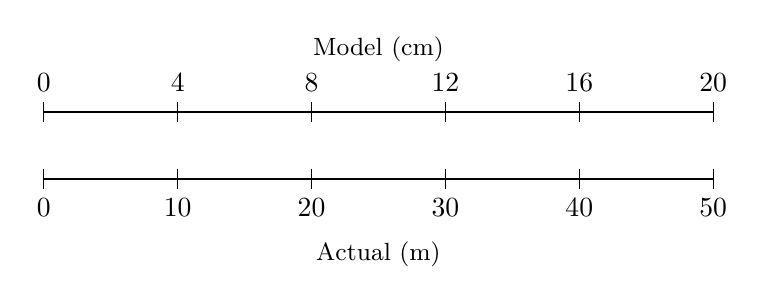
\begin{tikzpicture}[scale=0.85]
  \draw[thick] (0,0.5) -- (10,0.5);
  \draw[thick] (0,-0.5) -- (10,-0.5);
  \foreach \x/\lab in {0/0, 2/4, 4/8, 6/12, 8/16, 10/20}
    \draw (\x,0.35) -- (\x,0.65) node[above]{$\lab$};
  \node[above] at (5,1.1) {\small Model (cm)};
  \foreach \x/\lab in {0/0, 2/10, 4/20, 6/30, 8/40, 10/50}
    \draw (\x,-0.35) -- (\x,-0.65) node[below]{$\lab$};
  \node[below] at (5,-1.3) {\small Actual (m)};
\end{tikzpicture}
\end{center}

What actual length corresponds to a model length of $14$ cm?
\end{questionText}
\choiceA{$28$ m}
\choiceB{$35$ m}
\choiceC{$42$ m}
\choiceD{$70$ m}
\correctAnswer{B}
\explanation{From the double number line, the ratio is $\frac{10}{4} = 2.5$ m per cm. For $14$ cm: $14 \times 2.5 = 35$ m.}
\end{practiceQuestion}

\newpage
\section*{1-7-q25 \hfill \normalsize\texttt{tests\_questions\_bank\_2/topics\_additional/ch01-07-proportional-reasoning-with-scale-models.tex}}
\begin{practiceQuestion}{1-7-q25}{gsa}
\begin{questionText}
The scale drawing below shows the outline of a rectangular garden with a walkway across the middle.

\begin{center}
\begin{tikzpicture}[scale=0.8]
  \draw[thick,funGreen,fill=funGreen!10] (0,0) rectangle (6,4);
  \draw[thick,funOrange,fill=funOrange!20] (2.5,0) rectangle (3.5,4);
  \draw[<->,thick] (0,-0.5) -- (6,-0.5) node[midway,below]{\small $6$ cm};
  \draw[<->,thick] (-0.5,0) -- (-0.5,4) node[midway,left]{\small $4$ cm};
  \draw[<->,thick] (2.5,4.4) -- (3.5,4.4) node[midway,above]{\small $1$ cm};
  \node at (1.2,2) {\small Garden};
  \node[rotate=90] at (3,2) {\small Walk};
  \node at (0,-1.3) {};
  \node at (3,-1.3) {\small Scale: $1$ cm $= 3$ m};
\end{tikzpicture}
\end{center}

What is the actual area of the walkway in square meters?
\end{questionText}
\correctAnswer{$36$ sq m}
\explanation{Walkway on drawing: $1$ cm wide $\times$ $4$ cm long. Actual: width $= 1 \times 3 = 3$ m, length $= 4 \times 3 = 12$ m. Area $= 3 \times 12 = 36$ square meters.}
\end{practiceQuestion}

\newpage
\section*{1-7-q26 \hfill \normalsize\texttt{tests\_questions\_bank\_2/topics\_additional/ch01-07-proportional-reasoning-with-scale-models.tex}}
\begin{practiceQuestion}{1-7-q26}{gsa}
\begin{questionText}
The graph below shows the proportional relationship between model dimensions (cm) and actual dimensions (m) for a scale model.

\begin{center}
\begin{tikzpicture}[scale=0.5]
  \draw[step=1,gray!20,thin] (0,0) grid (10,10);
  \draw[thick,->] (0,0) -- (10.5,0) node[right]{\small Model (cm)};
  \draw[thick,->] (0,0) -- (0,10.5) node[above]{\small Actual (m)};
  \foreach \x in {2,4,6,8,10} \draw (\x,0.1) -- (\x,-0.1) node[below]{\tiny \x};
  \foreach \y in {2,4,6,8,10} \draw (0.1,\y) -- (-0.1,\y) node[left]{\tiny \y};
  \draw[thick,funBlue] (0,0) -- (10,8);
  \fill[funBlue] (0,0) circle (3pt);
  \fill[funBlue] (5,4) circle (3pt);
  \fill[funBlue] (10,8) circle (3pt);
\end{tikzpicture}
\end{center}

Using the graph, find the actual dimension for a model measurement of $15$ cm.
\end{questionText}
\correctAnswer{$12$ m}
\explanation{From the point $(5, 4)$: $k = \frac{4}{5} = 0.8$ m per cm. For $15$ cm: $0.8 \times 15 = 12$ m.}
\end{practiceQuestion}

\newpage
\section*{2-1-q22 \hfill \normalsize\texttt{tests\_questions\_bank\_2/topics/ch02-01-solving-percent-problems.tex}}
\begin{practiceQuestion}{2-1-q22}{gmc}
\begin{questionText}
The $10 \times 10$ grid below has some squares shaded. What percent of the grid is \textbf{not} shaded?

\begin{center}
\begin{tikzpicture}[scale=0.35]
  \foreach \x in {0,...,9} {
    \foreach \y in {0,...,9} {
      \draw[gray!50] (\x,\y) rectangle (\x+1,\y+1);
    }
  }
  % Shade 42 squares (rows 0-3 full = 40, plus 2 in row 4)
  \foreach \x in {0,...,9} {
    \foreach \y in {0,...,3} {
      \fill[funOrange!40] (\x,\y) rectangle (\x+1,\y+1);
      \draw[gray!50] (\x,\y) rectangle (\x+1,\y+1);
    }
  }
  \foreach \x in {0,...,1} {
    \fill[funOrange!40] (\x,4) rectangle (\x+1,5);
    \draw[gray!50] (\x,4) rectangle (\x+1,5);
  }
\end{tikzpicture}
\end{center}
\end{questionText}
\choiceA{$42\%$}
\choiceB{$48\%$}
\choiceC{$55\%$}
\choiceD{$58\%$}
\correctAnswer{D}
\explanation{The grid has $100$ squares. Shaded: $4$ full rows of $10 = 40$, plus $2$ more $= 42$. Not shaded: $100 - 42 = 58$. So $58\%$ is not shaded.}
\end{practiceQuestion}

\newpage
\section*{2-1-q24 \hfill \normalsize\texttt{tests\_questions\_bank\_2/topics/ch02-01-solving-percent-problems.tex}}
\begin{practiceQuestion}{2-1-q24}{gmc}
\begin{questionText}
The tape diagram below represents a whole quantity of $90$. What percent does the shaded section represent?

\begin{center}
\begin{tikzpicture}[scale=0.65]
  \foreach \i in {0,...,5} {
    \draw[thick] (\i*1.4,0) rectangle (\i*1.4+1.4,0.8);
  }
  \fill[funBlue!40] (0,0) rectangle (1.4,0.8);
  \fill[funBlue!40] (1.4,0) rectangle (2.8,0.8);
  \foreach \i in {0,...,5} {
    \draw[thick] (\i*1.4,0) rectangle (\i*1.4+1.4,0.8);
  }
  \node[below,font=\small] at (0.7,0) {$15$};
  \node[below,font=\small] at (2.1,0) {$15$};
  \node[below,font=\small] at (3.5,0) {$15$};
  \node[below,font=\small] at (4.9,0) {$15$};
  \node[below,font=\small] at (6.3,0) {$15$};
  \node[below,font=\small] at (7.7,0) {$15$};
  \draw[thick,<->] (0,-0.9) -- (8.4,-0.9) node[midway,below,font=\small] {Total $= 90$};
\end{tikzpicture}
\end{center}
\end{questionText}
\choiceA{$15\%$}
\choiceB{$20\%$}
\choiceC{$30\%$}
\choiceD{$\tfrac{100}{3}\%$}
\correctAnswer{D}
\explanation{Two out of six equal sections are shaded. The shaded part is $\frac{2}{6} = \frac{1}{3}$ of the whole. As a percent: $\frac{1}{3} \times 100 = 33.\overline{3}\%$, or $\frac{100}{3}\%$.}
\end{practiceQuestion}

\newpage
\section*{2-1-q25 \hfill \normalsize\texttt{tests\_questions\_bank\_2/topics/ch02-01-solving-percent-problems.tex}}
\begin{practiceQuestion}{2-1-q25}{gsa}
\begin{questionText}
The bar graph below shows the number of books read by four students in one month. What percent of the total books were read by Zoe?

\begin{center}
\begin{tikzpicture}[scale=0.5]
  \draw[thick,->] (0,0) -- (0,7) node[above]{\small Books};
  \draw[thick,->] (0,0) -- (9,0);
  \fill[funBlue!60] (0.5,0) rectangle (1.5,4);
  \fill[funGreen!60] (2.5,0) rectangle (3.5,6);
  \fill[funOrange!60] (4.5,0) rectangle (5.5,5);
  \fill[funRed!60] (6.5,0) rectangle (7.5,5);
  \node[below,font=\small] at (1,0) {Ava};
  \node[below,font=\small] at (3,0) {Zoe};
  \node[below,font=\small] at (5,0) {Leo};
  \node[below,font=\small] at (7,0) {Mia};
  \foreach \y/\lab in {1/2,2/4,3/6,4/8,5/10,6/12} {
    \draw (-0.1,\y) -- (0.1,\y) node[left,font=\small,xshift=-2pt] {\lab};
  }
  \node[above,font=\small] at (1,4) {$8$};
  \node[above,font=\small] at (3,6) {$12$};
  \node[above,font=\small] at (5,5) {$10$};
  \node[above,font=\small] at (7,5) {$10$};
\end{tikzpicture}
\end{center}
\end{questionText}
\correctAnswer{$30\%$}
\explanation{Total books: $8 + 12 + 10 + 10 = 40$. Zoe read $12$. Percent: $12 \div 40 = 0.30 = 30\%$.}
\end{practiceQuestion}

\newpage
\section*{2-1-q26 \hfill \normalsize\texttt{tests\_questions\_bank\_2/topics/ch02-01-solving-percent-problems.tex}}
\begin{practiceQuestion}{2-1-q26}{gsa}
\begin{questionText}
The circle graph below shows how a student spends $20$ hours each week on activities. How many hours does the student spend on homework?

\begin{center}
\begin{tikzpicture}[scale=1.2]
  % Pie chart: Sports 30%, Homework 25%, Video games 20%, Reading 25%
  \fill[funBlue!50] (0,0) -- (90:1) arc (90:198:1) -- cycle;
  \fill[funGreen!50] (0,0) -- (198:1) arc (198:270:1) -- cycle;
  \fill[funOrange!50] (0,0) -- (270:1) arc (270:360:1) -- cycle;
  \fill[funRed!50] (0,0) -- (0:1) arc (0:90:1) -- cycle;
  \draw (0,0) circle (1);
  \draw (0,0) -- (90:1); \draw (0,0) -- (198:1);
  \draw (0,0) -- (270:1); \draw (0,0) -- (0:1);
  \node[font=\small] at (144:0.65) {Sports};
  \node[font=\small] at (144:0.4) {$30\%$};
  \node[font=\small] at (234:0.65) {Games};
  \node[font=\small] at (234:0.4) {$20\%$};
  \node[font=\small] at (315:0.65) {Reading};
  \node[font=\small] at (315:0.4) {$25\%$};
  \node[font=\small] at (45:0.65) {HW};
  \node[font=\small] at (45:0.4) {$25\%$};
\end{tikzpicture}
\end{center}
\end{questionText}
\correctAnswer{$5$ hours}
\explanation{Homework is $25\%$ of the $20$ hours. Multiply: $0.25 \times 20 = 5$ hours on homework.}
\end{practiceQuestion}

\newpage
\section*{2-1-q27 \hfill \normalsize\texttt{tests\_questions\_bank\_2/topics/ch02-01-solving-percent-problems.tex}}
\begin{practiceQuestion}{2-1-q27}{gsa}
\begin{questionText}
The double number line below shows the relationship between a number and its percent. What value belongs at the question mark?

\begin{center}
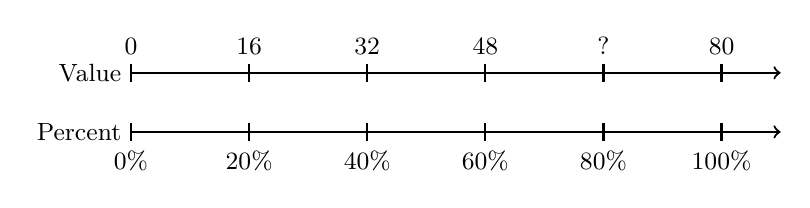
\begin{tikzpicture}[scale=0.75]
  \draw[thick,->] (0,1) -- (11,1);
  \node[left,font=\small] at (0,1) {Value};
  \foreach \x/\lab in {0/0, 2/16, 4/32, 6/48, 8/?, 10/80} {
    \draw[thick] (\x,0.85) -- (\x,1.15);
    \node[above,font=\small] at (\x,1.15) {\lab};
  }
  \draw[thick,->] (0,0) -- (11,0);
  \node[left,font=\small] at (0,0) {Percent};
  \foreach \x/\lab in {0/0\%, 2/20\%, 4/40\%, 6/60\%, 8/80\%, 10/100\%} {
    \draw[thick] (\x,-0.15) -- (\x,0.15);
    \node[below,font=\small] at (\x,-0.15) {\lab};
  }
\end{tikzpicture}
\end{center}
\end{questionText}
\correctAnswer{$64$}
\explanation{The whole ($100\%$) is $80$. The question mark is at $80\%$. Multiply: $0.80 \times 80 = 64$.}
\end{practiceQuestion}

\newpage
\section*{m-2-1-q23 \hfill \normalsize\texttt{tests\_questions\_bank\_2/topics\_modified/ch02-01-solving-percent-problems.tex}}
\begin{practiceQuestion}{m-2-1-q23}{gmc}
\begin{questionText}
The bar graph shows a family's monthly spending. What percent of their total spending goes to food?

\begin{center}
\begin{tikzpicture}[scale=0.5]
  \draw[thick,->] (0,0) -- (0,6) node[above]{\small Amount (\$)};
  \draw[thick,->] (0,0) -- (10,0);
  \fill[funBlue!60] (0.5,0) rectangle (2,5);
  \fill[funGreen!60] (2.5,0) rectangle (4,3);
  \fill[funOrange!60] (4.5,0) rectangle (6,1);
  \fill[funRed!60] (6.5,0) rectangle (8,1);
  \node[below,font=\small] at (1.25,0) {Housing};
  \node[below,font=\small] at (3.25,0) {Food};
  \node[below,font=\small] at (5.25,0) {Trans.};
  \node[below,font=\small] at (7.25,0) {Other};
  \foreach \y/\lab in {1/400,2/800,3/1200,4/1600,5/2000} {
    \draw (-0.1,\y) -- (0.1,\y) node[left,font=\small,xshift=-2pt] {\lab};
  }
  \node[above,font=\small] at (1.25,5) {$\$2{,}000$};
  \node[above,font=\small] at (3.25,3) {$\$1{,}200$};
  \node[above,font=\small] at (5.25,1) {$\$400$};
  \node[above,font=\small] at (7.25,1) {$\$400$};
\end{tikzpicture}
\end{center}
\end{questionText}
\choiceA{$20\%$}
\choiceB{$25\%$}
\choiceC{$30\%$}
\choiceD{$50\%$}
\correctAnswer{C}
\explanation{Total: $2{,}000 + 1{,}200 + 400 + 400 = \$4{,}000$. Food: $1{,}200 \div 4{,}000 = 0.30 = 30\%$.}
\end{practiceQuestion}

\newpage
\section*{m-2-1-q25 \hfill \normalsize\texttt{tests\_questions\_bank\_2/topics\_modified/ch02-01-solving-percent-problems.tex}}
\begin{practiceQuestion}{m-2-1-q25}{gsa}
\begin{questionText}
The tape diagram represents a $\$160$ purchase where a portion is the discount and the rest is the sale price. The discount is $35\%$. What is the sale price?

\begin{center}
\begin{tikzpicture}[scale=0.8]
  \draw[thick] (0,0) rectangle (8,0.8);
  \draw[thick] (2.8,0) -- (2.8,0.8);
  \fill[funRed!30] (0,0) rectangle (2.8,0.8);
  \fill[funGreen!30] (2.8,0) rectangle (8,0.8);
  \node[font=\small] at (1.4,0.4) {$35\%$};
  \node[font=\small] at (5.4,0.4) {$65\%$};
  \node[above,font=\small] at (4,0.8) {$\$160$ total};
\end{tikzpicture}
\end{center}
\end{questionText}
\correctAnswer{$\$104$}
\explanation{Sale price: $65\%$ of $\$160 = 0.65 \times 160 = \$104$.}
\end{practiceQuestion}

\newpage
\section*{m-2-1-q26 \hfill \normalsize\texttt{tests\_questions\_bank\_2/topics\_modified/ch02-01-solving-percent-problems.tex}}
\begin{practiceQuestion}{m-2-1-q26}{gsa}
\begin{questionText}
The circle graph shows how $200$ students chose their favorite sport. How many more chose basketball than soccer?

\begin{center}
\begin{tikzpicture}[scale=1.1]
  \fill[funBlue!50] (0,0) -- (90:1) arc (90:198:1) -- cycle;
  \fill[funGreen!50] (0,0) -- (198:1) arc (198:306:1) -- cycle;
  \fill[funOrange!50] (0,0) -- (306:1) arc (306:450:1) -- cycle;
  \draw (0,0) circle (1);
  \draw (0,0) -- (90:1); \draw (0,0) -- (198:1); \draw (0,0) -- (306:1);
  \node[font=\small] at (144:0.65) {Basketball};
  \node[font=\small] at (144:0.35) {$30\%$};
  \node[font=\small] at (252:0.65) {Soccer};
  \node[font=\small] at (252:0.35) {$30\%$};
  \node[font=\small] at (18:0.65) {Football};
  \node[font=\small] at (18:0.35) {$40\%$};
\end{tikzpicture}
\end{center}
\end{questionText}
\correctAnswer{$0$ (they are equal)}
\explanation{Basketball: $200 \times 0.30 = 60$. Soccer: $200 \times 0.30 = 60$. Difference: $60 - 60 = 0$. They are equal.}
\end{practiceQuestion}

\newpage
\section*{m-2-1-q27 \hfill \normalsize\texttt{tests\_questions\_bank\_2/topics\_modified/ch02-01-solving-percent-problems.tex}}
\begin{practiceQuestion}{m-2-1-q27}{gsa}
\begin{questionText}
The number line shows a price after a $20\%$ markup. The marked-up price is $\$72$. What was the original cost?

\begin{center}
\begin{tikzpicture}[scale=0.7]
  \draw[thick] (0,0) -- (10,0);
  \foreach \x/\lab in {0/$0$,2/$20$,4/$40$,6/$60$,8/$80$,10/$100$} {
    \draw (\x,-0.15) -- (\x,0.15);
    \node[below,font=\small] at (\x,-0.2) {\lab};
  }
  \draw[thick,funBlue,->] (7.2,0.8) -- (7.2,0.2);
  \node[above,font=\small,funBlue] at (7.2,0.8) {Selling: $\$72$};
  \draw[thick,funRed,->] (6,1.5) -- (6,0.2);
  \node[above,font=\small,funRed] at (6,1.5) {Original: ?};
\end{tikzpicture}
\end{center}
\end{questionText}
\correctAnswer{$\$60$}
\explanation{After a $20\%$ markup, selling price $= 1.20 \times P$. So $72 = 1.20P$ and $P = 72 \div 1.20 = \$60$.}
\end{practiceQuestion}

\newpage
\section*{2-2-q22 \hfill \normalsize\texttt{tests\_questions\_bank\_2/topics/ch02-02-connecting-percents-and-proportions.tex}}
\begin{practiceQuestion}{2-2-q22}{gmc}
\begin{questionText}
The double number line below shows a percent relationship. What number belongs at the question mark?

\begin{center}
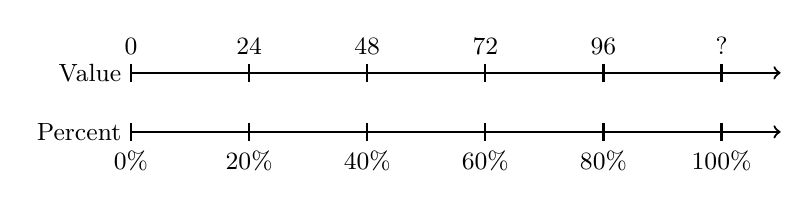
\begin{tikzpicture}[scale=0.75]
  \draw[thick,->] (0,1) -- (11,1);
  \node[left,font=\small] at (0,1) {Value};
  \foreach \x/\lab in {0/0, 2/24, 4/48, 6/72, 8/96, 10/?} {
    \draw[thick] (\x,0.85) -- (\x,1.15);
    \node[above,font=\small] at (\x,1.15) {\lab};
  }
  \draw[thick,->] (0,0) -- (11,0);
  \node[left,font=\small] at (0,0) {Percent};
  \foreach \x/\lab in {0/0\%, 2/20\%, 4/40\%, 6/60\%, 8/80\%, 10/100\%} {
    \draw[thick] (\x,-0.15) -- (\x,0.15);
    \node[below,font=\small] at (\x,-0.15) {\lab};
  }
\end{tikzpicture}
\end{center}
\end{questionText}
\choiceA{$100$}
\choiceB{$108$}
\choiceC{$112$}
\choiceD{$120$}
\correctAnswer{D}
\explanation{Each $20\%$ corresponds to $24$. At $100\%$: $24 \times 5 = 120$. Alternatively, if $20\%$ is $24$, the whole is $24 \div 0.20 = 120$.}
\end{practiceQuestion}

\newpage
\section*{2-2-q23 \hfill \normalsize\texttt{tests\_questions\_bank\_2/topics/ch02-02-connecting-percents-and-proportions.tex}}
\begin{practiceQuestion}{2-2-q23}{gmc}
\begin{questionText}
The bar model below is divided into $5$ equal sections. The total value is $160$. What percent of the total does the shaded part represent?

\begin{center}
\begin{tikzpicture}[scale=0.6]
  \foreach \i in {0,...,4} {
    \draw[thick] (\i*1.6,0) rectangle (\i*1.6+1.6,0.8);
  }
  \fill[funGreen!40] (0,0) rectangle (1.6,0.8);
  \fill[funGreen!40] (1.6,0) rectangle (3.2,0.8);
  \fill[funGreen!40] (3.2,0) rectangle (4.8,0.8);
  \foreach \i in {0,...,4} {
    \draw[thick] (\i*1.6,0) rectangle (\i*1.6+1.6,0.8);
  }
  \node[above,font=\small] at (2.4,0.8) {Shaded};
  \draw[thick,<->] (0,-0.5) -- (8,-0.5) node[midway,below,font=\small] {Total $= 160$};
\end{tikzpicture}
\end{center}
\end{questionText}
\choiceA{$30\%$}
\choiceB{$40\%$}
\choiceC{$50\%$}
\choiceD{$60\%$}
\correctAnswer{D}
\explanation{$3$ out of $5$ sections are shaded: $\frac{3}{5} = \frac{p}{100}$. Cross-multiply: $5p = 300$, so $p = 60\%$.}
\end{practiceQuestion}

\newpage
\section*{2-2-q25 \hfill \normalsize\texttt{tests\_questions\_bank\_2/topics/ch02-02-connecting-percents-and-proportions.tex}}
\begin{practiceQuestion}{2-2-q25}{gsa}
\begin{questionText}
The proportion model below shows two bars. Find the value of $n$.

\begin{center}
\begin{tikzpicture}[scale=0.6]
  \draw[thick] (0,1.5) rectangle (8,2.3);
  \fill[funBlue!40] (0,1.5) rectangle (5.6,2.3);
  \draw[thick] (0,1.5) rectangle (8,2.3);
  \draw[thick] (5.6,1.5) -- (5.6,2.3);
  \node[above,font=\small] at (2.8,2.3) {$n$};
  \node[right,font=\small] at (8.2,1.9) {$200$};
  \draw[thick] (0,0) rectangle (10,0.8);
  \fill[funBlue!40] (0,0) rectangle (7,0.8);
  \draw[thick] (0,0) rectangle (10,0.8);
  \draw[thick] (7,0) -- (7,0.8);
  \node[below,font=\small] at (3.5,0) {$70$};
  \node[right,font=\small] at (10.2,0.4) {$100$};
\end{tikzpicture}
\end{center}
\end{questionText}
\correctAnswer{$140$}
\explanation{$\frac{n}{200} = \frac{70}{100}$. Cross-multiply: $100n = 14{,}000$. Divide: $n = 140$.}
\end{practiceQuestion}

\newpage
\section*{2-2-q27 \hfill \normalsize\texttt{tests\_questions\_bank\_2/topics/ch02-02-connecting-percents-and-proportions.tex}}
\begin{practiceQuestion}{2-2-q27}{gsa}
\begin{questionText}
The number line below shows that the shaded region represents $45\%$ of the whole. If the shaded region has a value of $63$, what is the value of the whole?

\begin{center}
\begin{tikzpicture}[scale=0.7]
  \draw[thick] (0,0) -- (10,0);
  \draw[thick] (0,-0.2) -- (0,0.2) node[above,font=\small] {$0$};
  \draw[thick] (4.5,-0.2) -- (4.5,0.2) node[above,font=\small] {$63$};
  \draw[thick] (10,-0.2) -- (10,0.2) node[above,font=\small] {?};
  \fill[funBlue!30] (0,-0.1) rectangle (4.5,0.1);
  \node[below,font=\small] at (2.25,-0.3) {$45\%$};
  \node[below,font=\small] at (7.25,-0.3) {$55\%$};
\end{tikzpicture}
\end{center}
\end{questionText}
\correctAnswer{$140$}
\explanation{$\frac{63}{w} = \frac{45}{100}$. Cross-multiply: $45w = 6{,}300$. Divide: $w = 140$.}
\end{practiceQuestion}

\newpage
\section*{2-3-q22 \hfill \normalsize\texttt{tests\_questions\_bank\_2/topics/ch02-03-percent-increase-and-decrease.tex}}
\begin{practiceQuestion}{2-3-q22}{gmc}
\begin{questionText}
The bar graph shows the population of a town over two years. What is the percent increase from Year 1 to Year 2?

\begin{center}
\begin{tikzpicture}[scale=0.5]
  \draw[thick,->] (0,0) -- (0,7) node[above]{\small Population};
  \draw[thick,->] (0,0) -- (6,0);
  \fill[funBlue!60] (1,0) rectangle (2.5,5);
  \fill[funGreen!60] (3.5,0) rectangle (5,6);
  \node[below,font=\small] at (1.75,0) {Year 1};
  \node[below,font=\small] at (4.25,0) {Year 2};
  \foreach \y/\lab in {1/2000,2/4000,3/6000,4/8000,5/10000,6/12000} {
    \draw (-0.1,\y) -- (0.1,\y) node[left,font=\small,xshift=-2pt] {\lab};
  }
  \node[above,font=\small] at (1.75,5) {$10{,}000$};
  \node[above,font=\small] at (4.25,6) {$12{,}000$};
\end{tikzpicture}
\end{center}
\end{questionText}
\choiceA{$2\%$}
\choiceB{$12\%$}
\choiceC{$17\%$}
\choiceD{$20\%$}
\correctAnswer{D}
\explanation{Change: $12{,}000 - 10{,}000 = 2{,}000$. Percent increase: $2{,}000 \div 10{,}000 = 0.20 = 20\%$.}
\end{practiceQuestion}

\newpage
\section*{2-3-q24 \hfill \normalsize\texttt{tests\_questions\_bank\_2/topics/ch02-03-percent-increase-and-decrease.tex}}
\begin{practiceQuestion}{2-3-q24}{gmc}
\begin{questionText}
The number line below shows an original value and a new value. What is the percent decrease?

\begin{center}
\begin{tikzpicture}[scale=0.09]
  \draw[thick,->] (0,0) -- (105,0);
  \foreach \x in {0,10,...,100} {
    \draw (\x,1.5) -- (\x,-1.5) node[below,font=\small] {\x};
  }
  \fill[funRed] (90,0) circle (3) node[above=4pt,font=\small] {Original};
  \fill[funBlue] (72,0) circle (3) node[above=4pt,font=\small] {New};
  \draw[thick,->,funBlue] (88,4) -- (74,4);
\end{tikzpicture}
\end{center}
\end{questionText}
\choiceA{$18\%$}
\choiceB{$20\%$}
\choiceC{$25\%$}
\choiceD{$28\%$}
\correctAnswer{B}
\explanation{Change: $90 - 72 = 18$. Percent decrease: $18 \div 90 = 0.20 = 20\%$. Always divide by the original.}
\end{practiceQuestion}

\newpage
\section*{2-3-q25 \hfill \normalsize\texttt{tests\_questions\_bank\_2/topics/ch02-03-percent-increase-and-decrease.tex}}
\begin{practiceQuestion}{2-3-q25}{gsa}
\begin{questionText}
The bar graph shows the number of library visitors on two days. What is the percent increase from Monday to Tuesday?

\begin{center}
\begin{tikzpicture}[scale=0.5]
  \draw[thick,->] (0,0) -- (0,7) node[above]{\small Visitors};
  \draw[thick,->] (0,0) -- (6,0);
  \fill[funOrange!60] (1,0) rectangle (2.5,4);
  \fill[funBlue!60] (3.5,0) rectangle (5,5);
  \node[below,font=\small] at (1.75,0) {Mon};
  \node[below,font=\small] at (4.25,0) {Tue};
  \foreach \y/\lab in {1/30,2/60,3/90,4/120,5/150,6/180} {
    \draw (-0.1,\y) -- (0.1,\y) node[left,font=\small,xshift=-2pt] {\lab};
  }
  \node[above,font=\small] at (1.75,4) {$120$};
  \node[above,font=\small] at (4.25,5) {$150$};
\end{tikzpicture}
\end{center}
\end{questionText}
\correctAnswer{$25\%$}
\explanation{Change: $150 - 120 = 30$. Percent increase: $30 \div 120 = 0.25 = 25\%$.}
\end{practiceQuestion}

\newpage
\section*{2-3-q27 \hfill \normalsize\texttt{tests\_questions\_bank\_2/topics/ch02-03-percent-increase-and-decrease.tex}}
\begin{practiceQuestion}{2-3-q27}{gsa}
\begin{questionText}
The bar model below shows a price \textbf{before} and \textbf{after} a percent decrease. What was the percent decrease?

\begin{center}
\begin{tikzpicture}[scale=0.6]
  % Original bar
  \draw[thick] (0,1.2) rectangle (10,2);
  \fill[funBlue!30] (0,1.2) rectangle (10,2);
  \node[above,font=\small] at (5,2) {Original: $\$160$};
  % New bar
  \draw[thick] (0,0) rectangle (7,0.8);
  \fill[funGreen!30] (0,0) rectangle (7,0.8);
  \node[below,font=\small] at (3.5,0) {Sale: $\$112$};
  % Removed portion
  \draw[thick,dashed] (7,0) rectangle (10,0.8);
  \node[font=\small] at (8.5,0.4) {?};
\end{tikzpicture}
\end{center}
\end{questionText}
\correctAnswer{$30\%$}
\explanation{Change: $160 - 112 = 48$. Percent decrease: $48 \div 160 = 0.30 = 30\%$.}
\end{practiceQuestion}

\newpage
\section*{2-4-q22 \hfill \normalsize\texttt{tests\_questions\_bank\_2/topics/ch02-04-markups-discounts-and-sales-tax.tex}}
\begin{practiceQuestion}{2-4-q22}{gmc}
\begin{questionText}
The diagram shows the cost breakdown for a lamp. What is the percent markup?

\begin{center}
\begin{tikzpicture}[scale=0.6]
  % Cost bar
  \draw[thick] (0,0) rectangle (5,0.8);
  \fill[funBlue!40] (0,0) rectangle (5,0.8);
  \node[font=\small] at (2.5,0.4) {Cost: $\$40$};
  % Selling price bar
  \draw[thick] (0,1.5) rectangle (8.5,2.3);
  \fill[funGreen!40] (0,1.5) rectangle (5,2.3);
  \fill[funOrange!40] (5,1.5) rectangle (8.5,2.3);
  \draw[thick] (5,1.5) -- (5,2.3);
  \node[font=\small] at (2.5,1.9) {Cost};
  \node[font=\small] at (6.75,1.9) {Markup};
  \node[above,font=\small] at (4.25,2.3) {Selling Price: $\$68$};
\end{tikzpicture}
\end{center}
\end{questionText}
\choiceA{$28\%$}
\choiceB{$41\%$}
\choiceC{$58.8\%$}
\choiceD{$70\%$}
\correctAnswer{D}
\explanation{Markup amount: $68 - 40 = \$28$. Percent markup: $28 \div 40 = 0.70 = 70\%$.}
\end{practiceQuestion}

\newpage
\section*{2-4-q24 \hfill \normalsize\texttt{tests\_questions\_bank\_2/topics/ch02-04-markups-discounts-and-sales-tax.tex}}
\begin{practiceQuestion}{2-4-q24}{gmc}
\begin{questionText}
The bar model shows the flow from cost to final customer price. What is the sales tax rate?

\begin{center}
\begin{tikzpicture}[scale=0.55]
  % Cost bar
  \fill[funBlue!30] (0,2) rectangle (5,2.8);
  \draw[thick] (0,2) rectangle (5,2.8);
  \node[font=\small,above] at (2.5,2.8) {Cost: $\$50$};
  % After markup
  \fill[funGreen!30] (0,1) rectangle (7.5,1.8);
  \draw[thick] (0,1) rectangle (7.5,1.8);
  \node[font=\small,above] at (3.75,1.8) {After $50\%$ markup: $\$75$};
  % After tax
  \fill[funOrange!30] (0,0) rectangle (8.25,0.8);
  \draw[thick] (0,0) rectangle (8.25,0.8);
  \node[font=\small,below] at (4.125,0) {Final price: $\$81$};
\end{tikzpicture}
\end{center}
\end{questionText}
\choiceA{$6\%$}
\choiceB{$8\%$}
\choiceC{$10\%$}
\choiceD{$12\%$}
\correctAnswer{B}
\explanation{After markup: $\$75$. Tax amount: $81 - 75 = \$6$. Tax rate: $6 \div 75 = 0.08 = 8\%$.}
\end{practiceQuestion}

\newpage
\section*{2-4-q27 \hfill \normalsize\texttt{tests\_questions\_bank\_2/topics/ch02-04-markups-discounts-and-sales-tax.tex}}
\begin{practiceQuestion}{2-4-q27}{gsa}
\begin{questionText}
The diagram shows the price of a coat at every stage. What was the discount percent?

\begin{center}
\begin{tikzpicture}[scale=0.55]
  \node[draw,thick,rounded corners,fill=funBlue!15,minimum width=2.5cm,minimum height=0.8cm] (A) at (0,0) {Cost: $\$50$};
  \node[draw,thick,rounded corners,fill=funGreen!15,minimum width=2.5cm,minimum height=0.8cm] (B) at (5,0) {Retail: $\$85$};
  \node[draw,thick,rounded corners,fill=funOrange!15,minimum width=2.5cm,minimum height=0.8cm] (C) at (10,0) {Sale: $\$68$};
  \draw[thick,->] (A) -- (B) node[midway,above,font=\small] {$70\%$ markup};
  \draw[thick,->] (B) -- (C) node[midway,above,font=\small] {? discount};
\end{tikzpicture}
\end{center}
\end{questionText}
\correctAnswer{$20\%$}
\explanation{Discount amount: $85 - 68 = \$17$. Percent discount: $17 \div 85 = 0.20 = 20\%$.}
\end{practiceQuestion}

\newpage
\section*{2-5-q23 \hfill \normalsize\texttt{tests\_questions\_bank\_2/topics/ch02-05-tips-commissions-and-fees.tex}}
\begin{practiceQuestion}{2-5-q23}{gmc}
\begin{questionText}
The bar graph below shows a salesperson's monthly sales. If the commission rate is $6\%$, in which month did she earn the most commission?

\begin{center}
\begin{tikzpicture}[scale=0.45]
  \draw[thick,->] (0,0) -- (0,7) node[above]{\small Sales (\$)};
  \draw[thick,->] (0,0) -- (10,0);
  \fill[funBlue!60] (0.5,0) rectangle (2,4);
  \fill[funGreen!60] (2.5,0) rectangle (4,6);
  \fill[funOrange!60] (4.5,0) rectangle (6,3);
  \fill[funRed!60] (6.5,0) rectangle (8,5);
  \node[below,font=\small] at (1.25,0) {Jan};
  \node[below,font=\small] at (3.25,0) {Feb};
  \node[below,font=\small] at (5.25,0) {Mar};
  \node[below,font=\small] at (7.25,0) {Apr};
  \foreach \y/\lab in {1/2000,2/4000,3/6000,4/8000,5/10000,6/12000} {
    \draw (-0.1,\y) -- (0.1,\y) node[left,font=\small,xshift=-2pt] {\lab};
  }
  \node[above,font=\small] at (1.25,4) {$\$8{,}000$};
  \node[above,font=\small] at (3.25,6) {$\$12{,}000$};
  \node[above,font=\small] at (5.25,3) {$\$6{,}000$};
  \node[above,font=\small] at (7.25,5) {$\$10{,}000$};
\end{tikzpicture}
\end{center}
\end{questionText}
\choiceA{January ($\$480$)}
\choiceB{February ($\$720$)}
\choiceC{March ($\$360$)}
\choiceD{April ($\$600$)}
\correctAnswer{B}
\explanation{Commission is $6\%$ of sales. The highest sales month is February at $\$12{,}000$. Commission: $12{,}000 \times 0.06 = \$720$.}
\end{practiceQuestion}

\newpage
\section*{2-5-q26 \hfill \normalsize\texttt{tests\_questions\_bank\_2/topics/ch02-05-tips-commissions-and-fees.tex}}
\begin{practiceQuestion}{2-5-q26}{gsa}
\begin{questionText}
The pie chart shows how a $\$16$ tip was split among three servers. How much did Server B receive?

\begin{center}
\begin{tikzpicture}[scale=1.1]
  \fill[funBlue!50] (0,0) -- (90:1) arc (90:234:1) -- cycle;
  \fill[funGreen!50] (0,0) -- (234:1) arc (234:324:1) -- cycle;
  \fill[funOrange!50] (0,0) -- (324:1) arc (324:450:1) -- cycle;
  \draw (0,0) circle (1);
  \draw (0,0) -- (90:1); \draw (0,0) -- (234:1); \draw (0,0) -- (324:1);
  \node[font=\small] at (162:0.6) {A};
  \node[font=\small] at (162:0.35) {$40\%$};
  \node[font=\small] at (279:0.6) {B};
  \node[font=\small] at (279:0.35) {$25\%$};
  \node[font=\small] at (27:0.6) {C};
  \node[font=\small] at (27:0.35) {$35\%$};
\end{tikzpicture}
\end{center}
\end{questionText}
\correctAnswer{$\$4$}
\explanation{Server B gets $25\%$ of $\$16$: $0.25 \times 16 = \$4$.}
\end{practiceQuestion}

\newpage
\section*{2-5-q27 \hfill \normalsize\texttt{tests\_questions\_bank\_2/topics/ch02-05-tips-commissions-and-fees.tex}}
\begin{practiceQuestion}{2-5-q27}{gsa}
\begin{questionText}
The bar graph shows a salesperson's weekly sales over four weeks. If the commission rate is $5\%$, what was the total commission earned over the four weeks?

\begin{center}
\begin{tikzpicture}[scale=0.45]
  \draw[thick,->] (0,0) -- (0,7) node[above]{\small Sales (\$)};
  \draw[thick,->] (0,0) -- (10,0);
  \fill[funBlue!60] (0.5,0) rectangle (2,3);
  \fill[funGreen!60] (2.5,0) rectangle (4,5);
  \fill[funOrange!60] (4.5,0) rectangle (6,4);
  \fill[funRed!60] (6.5,0) rectangle (8,4);
  \node[below,font=\small] at (1.25,0) {Wk 1};
  \node[below,font=\small] at (3.25,0) {Wk 2};
  \node[below,font=\small] at (5.25,0) {Wk 3};
  \node[below,font=\small] at (7.25,0) {Wk 4};
  \foreach \y/\lab in {1/1000,2/2000,3/3000,4/4000,5/5000,6/6000} {
    \draw (-0.1,\y) -- (0.1,\y) node[left,font=\small,xshift=-2pt] {\lab};
  }
  \node[above,font=\small] at (1.25,3) {$\$3{,}000$};
  \node[above,font=\small] at (3.25,5) {$\$5{,}000$};
  \node[above,font=\small] at (5.25,4) {$\$4{,}000$};
  \node[above,font=\small] at (7.25,4) {$\$4{,}000$};
\end{tikzpicture}
\end{center}
\end{questionText}
\correctAnswer{$\$800$}
\explanation{Total sales: $3{,}000 + 5{,}000 + 4{,}000 + 4{,}000 = \$16{,}000$. Commission: $16{,}000 \times 0.05 = \$800$.}
\end{practiceQuestion}

\newpage
\section*{2-6-q23 \hfill \normalsize\texttt{tests\_questions\_bank\_2/topics/ch02-06-simple-interest.tex}}
\begin{practiceQuestion}{2-6-q23}{gmc}
\begin{questionText}
The line graph shows the total amount in a simple interest savings account over time. What is the annual interest rate?

\begin{center}
\begin{tikzpicture}[scale=0.7]
  \draw[thick,->] (0,0) -- (6,0) node[right]{\small Years};
  \draw[thick,->] (0,0) -- (0,5.5) node[above]{\small Amount (\$)};
  \foreach \x in {0,...,5} {
    \draw (\x,-0.1) -- (\x,0.1) node[below=3pt,font=\small] {\x};
  }
  \foreach \y/\lab in {1/200,2/400,3/600,4/800,5/1000} {
    \draw (-0.1,\y) -- (0.1,\y) node[left,font=\small,xshift=-2pt] {\lab};
  }
  \draw[thick,funBlue,mark=*,mark size=2pt] plot coordinates {(0,2.5) (1,2.75) (2,3) (3,3.25) (4,3.5) (5,3.75)};
  \node[right,font=\small,funBlue] at (5,3.75) {$\$750$};
  \node[left,font=\small,funBlue] at (0,2.5) {$\$500$};
\end{tikzpicture}
\end{center}
\end{questionText}
\choiceA{$5\%$}
\choiceB{$8\%$}
\choiceC{$10\%$}
\choiceD{$25\%$}
\correctAnswer{C}
\explanation{Principal: $\$500$. After $5$ years: $\$750$. Interest: $750 - 500 = \$250$. Rate: $250 \div (500 \times 5) = 250 \div 2{,}500 = 0.10 = 10\%$.}
\end{practiceQuestion}

\newpage
\section*{2-6-q24 \hfill \normalsize\texttt{tests\_questions\_bank\_2/topics/ch02-06-simple-interest.tex}}
\begin{practiceQuestion}{2-6-q24}{gmc}
\begin{questionText}
The bar graph compares the interest earned by two accounts over the same period. Account A has $\$2{,}000$ at $3\%$. Account B has $\$1{,}000$ at what rate, if both earn the same interest after $4$ years?

\begin{center}
\begin{tikzpicture}[scale=0.5]
  \draw[thick,->] (0,0) -- (0,5.5) node[above]{\small Interest (\$)};
  \draw[thick,->] (0,0) -- (6,0);
  \fill[funBlue!60] (0.75,0) rectangle (2.25,4);
  \fill[funGreen!60] (3.25,0) rectangle (4.75,4);
  \node[below,font=\small] at (1.5,0) {Acct A};
  \node[below,font=\small] at (4,0) {Acct B};
  \foreach \y/\lab in {1/60,2/120,3/180,4/240} {
    \draw (-0.1,\y) -- (0.1,\y) node[left,font=\small,xshift=-2pt] {\lab};
  }
  \node[above,font=\small] at (1.5,4) {$\$240$};
  \node[above,font=\small] at (4,4) {$\$240$};
\end{tikzpicture}
\end{center}
\end{questionText}
\choiceA{$3\%$}
\choiceB{$4\%$}
\choiceC{$6\%$}
\choiceD{$8\%$}
\correctAnswer{C}
\explanation{Account A: $2{,}000 \times 0.03 \times 4 = \$240$. Account B: $240 = 1{,}000 \times r \times 4$, so $4{,}000r = 240$ and $r = 0.06 = 6\%$.}
\end{practiceQuestion}

\newpage
\section*{2-6-q25 \hfill \normalsize\texttt{tests\_questions\_bank\_2/topics/ch02-06-simple-interest.tex}}
\begin{practiceQuestion}{2-6-q25}{gsa}
\begin{questionText}
The timeline below shows a loan. Find the total amount owed at the end.

\begin{center}
\begin{tikzpicture}[scale=0.9]
  \draw[thick,->] (0,0) -- (8,0);
  \foreach \x/\lab in {0/Year 0, 2/Year 1, 4/Year 2, 6/Year 3} {
    \draw (\x,-0.15) -- (\x,0.15);
    \node[below,font=\small] at (\x,-0.2) {\lab};
  }
  \node[above,font=\small] at (0,0.3) {Borrow $\$3{,}000$};
  \node[above,font=\small] at (3,0.8) {Rate: $5\%$/year};
  \node[above,font=\small] at (6,0.3) {Total $= \,?$};
\end{tikzpicture}
\end{center}
\end{questionText}
\correctAnswer{$\$3{,}450$}
\explanation{$I = 3{,}000 \times 0.05 \times 3 = \$450$. Total: $3{,}000 + 450 = \$3{,}450$.}
\end{practiceQuestion}

\newpage
\section*{2-6-q27 \hfill \normalsize\texttt{tests\_questions\_bank\_2/topics/ch02-06-simple-interest.tex}}
\begin{practiceQuestion}{2-6-q27}{gsa}
\begin{questionText}
The bar graph below shows the interest earned each year on a $\$1{,}000$ deposit. Since simple interest is the same each year, how many years does it take to earn a total of $\$350$?

\begin{center}
\begin{tikzpicture}[scale=0.55]
  \draw[thick,->] (0,0) -- (0,4.5) node[above]{\small Interest (\$)};
  \draw[thick,->] (0,0) -- (5,0);
  \fill[funOrange!60] (1,0) rectangle (2.5,3.5);
  \node[below,font=\small] at (1.75,0) {Year 1};
  \node[above,font=\small] at (1.75,3.5) {$\$70$};
  \foreach \y/\lab in {1/20,2/40,3/60,3.5/70} {
    \draw (-0.1,\y) -- (0.1,\y) node[left,font=\small,xshift=-2pt] {\lab};
  }
  \node[font=\small] at (3.5,2) {Same each year};
\end{tikzpicture}
\end{center}
\end{questionText}
\correctAnswer{$5$ years}
\explanation{Each year earns $\$70$. To reach $\$350$: $350 \div 70 = 5$ years.}
\end{practiceQuestion}

\newpage
\section*{m-2-6-q23 \hfill \normalsize\texttt{tests\_questions\_bank\_2/topics\_modified/ch02-06-simple-interest.tex}}
\begin{practiceQuestion}{m-2-6-q23}{gmc}
\begin{questionText}
The line graph shows the total balance of a $\$2{,}000$ deposit earning simple interest. What is the annual interest rate?

\begin{center}
\begin{tikzpicture}[scale=0.7]
  \draw[thick,->] (0,0) -- (6,0) node[right]{\small Years};
  \draw[thick,->] (0,0) -- (0,5.5) node[above]{\small Balance (\$)};
  \foreach \x in {0,...,5} {
    \draw (\x,-0.1) -- (\x,0.1) node[below=3pt,font=\small] {\x};
  }
  \foreach \y/\lab in {1/500,2/1000,3/1500,4/2000,5/2500} {
    \draw (-0.1,\y) -- (0.1,\y) node[left,font=\small,xshift=-2pt] {\lab};
  }
  \draw[thick,funGreen,mark=*,mark size=2pt] plot coordinates {(0,4) (1,4.16) (2,4.32) (3,4.48) (4,4.64)};
  \node[left,font=\small,funGreen] at (0,4) {$\$2{,}000$};
  \node[right,font=\small,funGreen] at (4,4.64) {$\$2{,}320$};
\end{tikzpicture}
\end{center}
\end{questionText}
\choiceA{$2\%$}
\choiceB{$3\%$}
\choiceC{$4\%$}
\choiceD{$8\%$}
\correctAnswer{C}
\explanation{Interest over $4$ years: $2{,}320 - 2{,}000 = \$320$. Rate: $320 \div (2{,}000 \times 4) = 320 \div 8{,}000 = 0.04 = 4\%$.}
\end{practiceQuestion}

\newpage
\section*{m-2-6-q24 \hfill \normalsize\texttt{tests\_questions\_bank\_2/topics\_modified/ch02-06-simple-interest.tex}}
\begin{practiceQuestion}{m-2-6-q24}{gmc}
\begin{questionText}
The bar graph compares interest earned by savings vs.\ borrowing at the same rate. A person deposits $\$1{,}000$ (savings) and borrows $\$1{,}000$ (loan) both at $5\%$ for $3$ years. Which statement is true?

\begin{center}
\begin{tikzpicture}[scale=0.5]
  \draw[thick,->] (0,0) -- (0,5) node[above]{\small Interest (\$)};
  \draw[thick,->] (0,0) -- (6,0);
  \fill[funGreen!60] (0.75,0) rectangle (2.25,3);
  \fill[funRed!60] (3.25,0) rectangle (4.75,3);
  \node[below,font=\small] at (1.5,0) {Earned};
  \node[below,font=\small] at (4,0) {Owed};
  \foreach \y/\lab in {1/50,2/100,3/150,4/200} {
    \draw (-0.1,\y) -- (0.1,\y) node[left,font=\small,xshift=-2pt] {\lab};
  }
  \node[above,font=\small] at (1.5,3) {$\$150$};
  \node[above,font=\small] at (4,3) {$\$150$};
\end{tikzpicture}
\end{center}
\end{questionText}
\choiceA{You earn more than you owe}
\choiceB{You owe more than you earn}
\choiceC{Earned and owed interest are equal at the same rate, principal, and time}
\choiceD{The borrower pays no interest}
\correctAnswer{C}
\explanation{Both use $I = 1{,}000 \times 0.05 \times 3 = \$150$. The formula gives the same result whether you save or borrow.}
\end{practiceQuestion}

\newpage
\section*{m-2-6-q25 \hfill \normalsize\texttt{tests\_questions\_bank\_2/topics\_modified/ch02-06-simple-interest.tex}}
\begin{practiceQuestion}{m-2-6-q25}{gsa}
\begin{questionText}
The timeline shows a savings deposit. Find the total amount at the end.

\begin{center}
\begin{tikzpicture}[scale=0.9]
  \draw[thick,->] (0,0) -- (10,0);
  \foreach \x/\lab in {0/Year 0, 2/Year 1, 4/Year 2, 6/Year 3, 8/Year 4} {
    \draw (\x,-0.15) -- (\x,0.15);
    \node[below,font=\small] at (\x,-0.2) {\lab};
  }
  \node[above,font=\small] at (0,0.3) {Deposit $\$5{,}000$};
  \node[above,font=\small] at (4,0.8) {Rate: $3\%$/year};
  \node[above,font=\small] at (8,0.3) {Total $= \,?$};
\end{tikzpicture}
\end{center}
\end{questionText}
\correctAnswer{$\$5{,}600$}
\explanation{$I = 5{,}000 \times 0.03 \times 4 = \$600$. Total: $5{,}000 + 600 = \$5{,}600$.}
\end{practiceQuestion}

\newpage
\section*{m-2-6-q27 \hfill \normalsize\texttt{tests\_questions\_bank\_2/topics\_modified/ch02-06-simple-interest.tex}}
\begin{practiceQuestion}{m-2-6-q27}{gsa}
\begin{questionText}
The bar graph shows the interest earned per year on a $\$6{,}000$ deposit. Each year earns the same interest. How many years does it take to earn $\$900$ total?

\begin{center}
\begin{tikzpicture}[scale=0.55]
  \draw[thick,->] (0,0) -- (0,4.5) node[above]{\small Interest (\$)};
  \draw[thick,->] (0,0) -- (5,0);
  \fill[funBlue!60] (1,0) rectangle (2.5,3);
  \node[below,font=\small] at (1.75,0) {Year 1};
  \node[above,font=\small] at (1.75,3) {$\$150$};
  \foreach \y/\lab in {1/50,2/100,3/150,4/200} {
    \draw (-0.1,\y) -- (0.1,\y) node[left,font=\small,xshift=-2pt] {\lab};
  }
  \node[font=\small] at (3.5,2) {Same each year};
\end{tikzpicture}
\end{center}
\end{questionText}
\correctAnswer{$6$ years}
\explanation{Each year: $\$150$. To reach $\$900$: $900 \div 150 = 6$ years.}
\end{practiceQuestion}

\newpage
\section*{2-7-q23 \hfill \normalsize\texttt{tests\_questions\_bank\_2/topics/ch02-07-percent-error.tex}}
\begin{practiceQuestion}{2-7-q23}{gmc}
\begin{questionText}
The bar graph shows a student's estimated and actual quiz scores over four quizzes. On which quiz was the percent error the largest?

\begin{center}
\begin{tikzpicture}[scale=0.5]
  \draw[thick,->] (0,0) -- (0,6) node[above]{\small Score};
  \draw[thick,->] (0,0) -- (11,0);
  % Quiz 1
  \fill[funBlue!40] (0.5,0) rectangle (1.5,4);
  \fill[funBlue!80] (1.5,0) rectangle (2.5,5);
  % Quiz 2
  \fill[funBlue!40] (3,0) rectangle (4,3);
  \fill[funBlue!80] (4,0) rectangle (5,4);
  % Quiz 3
  \fill[funBlue!40] (5.5,0) rectangle (6.5,4.5);
  \fill[funBlue!80] (6.5,0) rectangle (7.5,4);
  % Quiz 4
  \fill[funBlue!40] (8,0) rectangle (9,5);
  \fill[funBlue!80] (9,0) rectangle (10,5);
  \node[below,font=\small] at (1.5,0) {Q1};
  \node[below,font=\small] at (4,0) {Q2};
  \node[below,font=\small] at (6.5,0) {Q3};
  \node[below,font=\small] at (9,0) {Q4};
  \node[above,font=\tiny] at (1,4) {80};
  \node[above,font=\tiny] at (2,5) {100};
  \node[above,font=\tiny] at (3.5,3) {60};
  \node[above,font=\tiny] at (4.5,4) {80};
  \node[above,font=\tiny] at (6,4.5) {90};
  \node[above,font=\tiny] at (7,4) {80};
  \node[above,font=\tiny] at (8.5,5) {100};
  \node[above,font=\tiny] at (9.5,5) {100};
  \foreach \y/\lab in {1/20,2/40,3/60,4/80,5/100} {
    \draw (-0.1,\y) -- (0.1,\y) node[left,font=\small,xshift=-2pt] {\lab};
  }
  \node[font=\small] at (11.5,4.5) {\textcolor{funBlue!40}{Est.}};
  \node[font=\small] at (11.5,3.5) {\textcolor{funBlue!80}{Act.}};
\end{tikzpicture}
\end{center}
\end{questionText}
\choiceA{Quiz 1 ($20\%$)}
\choiceB{Quiz 2 ($25\%$)}
\choiceC{Quiz 3 ($12.5\%$)}
\choiceD{Quiz 4 ($0\%$)}
\correctAnswer{B}
\explanation{Q1: $\frac{|80-100|}{100} = 20\%$. Q2: $\frac{|60-80|}{80} = 25\%$. Q3: $\frac{|90-80|}{80} = 12.5\%$. Q4: $0\%$. Quiz 2 is highest.}
\end{practiceQuestion}

\newpage
\section*{2-7-q24 \hfill \normalsize\texttt{tests\_questions\_bank\_2/topics/ch02-07-percent-error.tex}}
\begin{practiceQuestion}{2-7-q24}{gmc}
\begin{questionText}
A number line shows an estimated measurement and the actual measurement. What is the percent error?

\begin{center}
\begin{tikzpicture}[scale=0.8]
  \draw[thick] (0,0) -- (10,0);
  \foreach \x/\lab in {0/0,2/20,4/40,6/60,8/80,10/100} {
    \draw (\x,-0.15) -- (\x,0.15);
    \node[below,font=\small] at (\x,-0.2) {\lab};
  }
  \draw[thick,funRed,->] (7,0.8) -- (7,0.2);
  \node[above,font=\small,funRed] at (7,0.8) {Estimated: 70};
  \draw[thick,funBlue,->] (8,0.8) -- (8,0.2);
  \node[above,font=\small,funBlue] at (8,0.8) {Actual: 80};
\end{tikzpicture}
\end{center}
\end{questionText}
\choiceA{$10\%$}
\choiceB{$12.5\%$}
\choiceC{$14.3\%$}
\choiceD{$20\%$}
\correctAnswer{B}
\explanation{$\dfrac{|70 - 80|}{80} \times 100 = \dfrac{10}{80} \times 100 = 12.5\%$.}
\end{practiceQuestion}

\newpage
\section*{2-7-q26 \hfill \normalsize\texttt{tests\_questions\_bank\_2/topics/ch02-07-percent-error.tex}}
\begin{practiceQuestion}{2-7-q26}{gsa}
\begin{questionText}
The double bar graph compares estimated and actual temperatures for three cities. Find the percent error for City B (to the nearest tenth).

\begin{center}
\begin{tikzpicture}[scale=0.45]
  \draw[thick,->] (0,0) -- (0,7) node[above]{\small Temp (\textdegree F)};
  \draw[thick,->] (0,0) -- (10,0);
  % City A
  \fill[funRed!40] (0.5,0) rectangle (1.5,5);
  \fill[funRed!80] (1.5,0) rectangle (2.5,4);
  % City B
  \fill[funRed!40] (3.5,0) rectangle (4.5,4.5);
  \fill[funRed!80] (4.5,0) rectangle (5.5,6);
  % City C
  \fill[funRed!40] (6.5,0) rectangle (7.5,3);
  \fill[funRed!80] (7.5,0) rectangle (8.5,3);
  \node[below,font=\small] at (1.5,0) {A};
  \node[below,font=\small] at (4.5,0) {B};
  \node[below,font=\small] at (7.5,0) {C};
  \foreach \y/\lab in {1/10,2/20,3/30,4/40,5/50,6/60} {
    \draw (-0.1,\y) -- (0.1,\y) node[left,font=\small,xshift=-2pt] {\lab};
  }
  \node[above,font=\tiny] at (1,5) {50};
  \node[above,font=\tiny] at (2,4) {40};
  \node[above,font=\tiny] at (4,4.5) {45};
  \node[above,font=\tiny] at (5,6) {60};
  \node[above,font=\tiny] at (7,3) {30};
  \node[above,font=\tiny] at (8,3) {30};
  \node[font=\small] at (10,5.5) {\textcolor{funRed!40}{Est.}};
  \node[font=\small] at (10,4.5) {\textcolor{funRed!80}{Act.}};
\end{tikzpicture}
\end{center}
\end{questionText}
\correctAnswer{$25\%$}
\explanation{City B: Est. $= 45$, Act. $= 60$. $\dfrac{|45 - 60|}{60} \times 100 = \dfrac{15}{60} \times 100 = 25\%$.}
\end{practiceQuestion}

\newpage
\section*{2-8-q23 \hfill \normalsize\texttt{tests\_questions\_bank\_2/topics\_additional/ch02-08-personal-financial-literacy.tex}}
\begin{practiceQuestion}{2-8-q23}{gmc}
\begin{questionText}
The bar graph compares interest charged on a $\$1{,}000$ balance at two different annual rates over one year. What is the monthly interest for Card B?

\begin{center}
\begin{tikzpicture}[scale=0.5]
  \draw[thick,->] (0,0) -- (0,6) node[above]{\small Annual Interest (\$)};
  \draw[thick,->] (0,0) -- (6,0);
  \fill[funBlue!60] (0.75,0) rectangle (2.25,3);
  \fill[funRed!60] (3.25,0) rectangle (4.75,4.5);
  \node[below,font=\small] at (1.5,0) {Card A};
  \node[below,font=\small] at (4,0) {Card B};
  \foreach \y/\lab in {1.5/150,3/300,4.5/450} {
    \draw (-0.1,\y) -- (0.1,\y) node[left,font=\small,xshift=-2pt] {$\$\lab$};
  }
  \node[above,font=\small] at (1.5,3) {$15\%$};
  \node[above,font=\small] at (4,4.5) {$22.5\%$};
\end{tikzpicture}
\end{center}
\end{questionText}
\choiceA{$\$12.50$}
\choiceB{$\$18.75$}
\choiceC{$\$22.50$}
\choiceD{$\$37.50$}
\correctAnswer{B}
\explanation{Card B annual: $1{,}000 \times 0.225 = \$225$. Monthly: $225 \div 12 = \$18.75$.}
\end{practiceQuestion}

\newpage
\section*{2-8-q26 \hfill \normalsize\texttt{tests\_questions\_bank\_2/topics\_additional/ch02-08-personal-financial-literacy.tex}}
\begin{practiceQuestion}{2-8-q26}{gsa}
\begin{questionText}
The pie chart shows how a $\$24$ monthly bank fee is divided. How much goes to the ATM fee category?

\begin{center}
\begin{tikzpicture}[scale=1.1]
  \fill[funBlue!50] (0,0) -- (90:1) arc (90:234:1) -- cycle;
  \fill[funGreen!50] (0,0) -- (234:1) arc (234:306:1) -- cycle;
  \fill[funOrange!50] (0,0) -- (306:1) arc (306:450:1) -- cycle;
  \draw (0,0) circle (1);
  \draw (0,0) -- (90:1); \draw (0,0) -- (234:1); \draw (0,0) -- (306:1);
  \node[font=\small] at (162:0.6) {Maint.};
  \node[font=\small] at (162:0.35) {$40\%$};
  \node[font=\small] at (270:0.55) {ATM};
  \node[font=\small] at (270:0.3) {$20\%$};
  \node[font=\small] at (18:0.6) {Other};
  \node[font=\small] at (18:0.35) {$40\%$};
\end{tikzpicture}
\end{center}
\end{questionText}
\correctAnswer{$\$4.80$}
\explanation{ATM portion: $20\%$ of $\$24 = 0.20 \times 24 = \$4.80$.}
\end{practiceQuestion}

\newpage
\section*{2-9-q22 \hfill \normalsize\texttt{tests\_questions\_bank\_2/topics\_additional/ch02-09-financial-literacy-budgeting-saving-and-investing.tex}}
\begin{practiceQuestion}{2-9-q22}{gmc}
\begin{questionText}
The pie chart shows a family's monthly budget. If their income is $\$4{,}000$, how much goes to housing?

\begin{center}
\begin{tikzpicture}[scale=1.1]
  \fill[funBlue!50] (0,0) -- (90:1) arc (90:198:1) -- cycle;
  \fill[funGreen!50] (0,0) -- (198:1) arc (198:270:1) -- cycle;
  \fill[funOrange!50] (0,0) -- (270:1) arc (270:342:1) -- cycle;
  \fill[funRed!50] (0,0) -- (342:1) arc (342:450:1) -- cycle;
  \draw (0,0) circle (1);
  \draw (0,0) -- (90:1); \draw (0,0) -- (198:1); \draw (0,0) -- (270:1); \draw (0,0) -- (342:1);
  \node[font=\small] at (144:0.65) {Housing};
  \node[font=\small] at (144:0.35) {$30\%$};
  \node[font=\small] at (234:0.65) {Food};
  \node[font=\small] at (234:0.35) {$20\%$};
  \node[font=\small] at (306:0.6) {Transport};
  \node[font=\small] at (306:0.35) {$20\%$};
  \node[font=\small] at (36:0.65) {Other};
  \node[font=\small] at (36:0.35) {$30\%$};
\end{tikzpicture}
\end{center}
\end{questionText}
\choiceA{$\$800$}
\choiceB{$\$1{,}000$}
\choiceC{$\$1{,}200$}
\choiceD{$\$1{,}500$}
\correctAnswer{C}
\explanation{Housing: $30\%$ of $\$4{,}000 = 0.30 \times 4{,}000 = \$1{,}200$.}
\end{practiceQuestion}

\newpage
\section*{2-9-q23 \hfill \normalsize\texttt{tests\_questions\_bank\_2/topics\_additional/ch02-09-financial-literacy-budgeting-saving-and-investing.tex}}
\begin{practiceQuestion}{2-9-q23}{gmc}
\begin{questionText}
The bar graph shows a student's spending by category over one month. If her total income was $\$500$, what percent went to savings?

\begin{center}
\begin{tikzpicture}[scale=0.5]
  \draw[thick,->] (0,0) -- (0,6) node[above]{\small Amount (\$)};
  \draw[thick,->] (0,0) -- (10,0);
  \fill[funBlue!60] (0.5,0) rectangle (2,4);
  \fill[funGreen!60] (2.5,0) rectangle (4,3);
  \fill[funOrange!60] (4.5,0) rectangle (6,1.5);
  \fill[funRed!60] (6.5,0) rectangle (8,1.5);
  \node[below,font=\small] at (1.25,0) {Food};
  \node[below,font=\small] at (3.25,0) {Fun};
  \node[below,font=\small] at (5.25,0) {Trans.};
  \node[below,font=\small] at (7.25,0) {Other};
  \foreach \y/\lab in {1/50,2/100,3/150,4/200,5/250} {
    \draw (-0.1,\y) -- (0.1,\y) node[left,font=\small,xshift=-2pt] {\lab};
  }
  \node[above,font=\small] at (1.25,4) {$\$200$};
  \node[above,font=\small] at (3.25,3) {$\$150$};
  \node[above,font=\small] at (5.25,1.5) {$\$75$};
  \node[above,font=\small] at (7.25,1.5) {$\$25$};
\end{tikzpicture}
\end{center}
\end{questionText}
\choiceA{$5\%$}
\choiceB{$10\%$}
\choiceC{$15\%$}
\choiceD{$20\%$}
\correctAnswer{B}
\explanation{Total spent: $200 + 150 + 75 + 25 = \$450$. Savings: $500 - 450 = \$50$. Rate: $50 \div 500 = 0.10 = 10\%$.}
\end{practiceQuestion}

\newpage
\section*{2-9-q26 \hfill \normalsize\texttt{tests\_questions\_bank\_2/topics\_additional/ch02-09-financial-literacy-budgeting-saving-and-investing.tex}}
\begin{practiceQuestion}{2-9-q26}{gsa}
\begin{questionText}
The line graph shows a student's savings balance over $5$ months. How much did the student save per month on average?

\begin{center}
\begin{tikzpicture}[scale=0.7]
  \draw[thick,->] (0,0) -- (6,0) node[right]{\small Month};
  \draw[thick,->] (0,0) -- (0,5.5) node[above]{\small Balance (\$)};
  \foreach \x/\lab in {0/0,1/1,2/2,3/3,4/4,5/5} {
    \draw (\x,-0.1) -- (\x,0.1) node[below=3pt,font=\small] {\lab};
  }
  \foreach \y/\lab in {1/100,2/200,3/300,4/400,5/500} {
    \draw (-0.1,\y) -- (0.1,\y) node[left,font=\small,xshift=-2pt] {\lab};
  }
  \draw[thick,funGreen,mark=*,mark size=2pt] plot coordinates {(0,0.5) (1,1.2) (2,2) (3,2.8) (4,3.5) (5,4.5)};
  \node[right,font=\small,funGreen] at (5,4.5) {$\$450$};
  \node[left,font=\small,funGreen] at (0,0.5) {$\$50$};
\end{tikzpicture}
\end{center}
\end{questionText}
\correctAnswer{$\$80$}
\explanation{Net savings: $450 - 50 = \$400$ over $5$ months. Average: $400 \div 5 = \$80$ per month.}
\end{practiceQuestion}

\newpage
\section*{2-10-q23 \hfill \normalsize\texttt{tests\_questions\_bank\_2/topics\_additional/ch02-10-compound-interest-introduction.tex}}
\begin{practiceQuestion}{2-10-q23}{gmc}
\begin{questionText}
The bar graph compares the total amount after $2$ years for simple and compound interest on a $\$2{,}000$ deposit at $5\%$. Which bar shows the compound interest total?

\begin{center}
\begin{tikzpicture}[scale=0.5]
  \draw[thick,->] (0,0) -- (0,6) node[above]{\small Total (\$)};
  \draw[thick,->] (0,0) -- (6,0);
  \fill[funBlue!60] (0.75,0) rectangle (2.25,4);
  \fill[funGreen!60] (3.25,0) rectangle (4.75,4.1);
  \node[below,font=\small] at (1.5,0) {A};
  \node[below,font=\small] at (4,0) {B};
  \foreach \y/\lab in {2/2100,4/2200,4.1/2205} {
    \draw (-0.1,\y) -- (0.1,\y);
  }
  \node[left,font=\small] at (-0.1,4) {$\$2{,}200$};
  \node[above,font=\small] at (1.5,4) {$\$2{,}200$};
  \node[above,font=\small] at (4,4.1) {$\$2{,}205$};
\end{tikzpicture}
\end{center}
\end{questionText}
\choiceA{Bar A ($\$2{,}200$)}
\choiceB{Bar B ($\$2{,}205$)}
\choiceC{Both are compound}
\choiceD{Neither is compound}
\correctAnswer{B}
\explanation{Simple: $2{,}000 + 200 = \$2{,}200$ (Bar A). Compound: $2{,}000(1.05)^2 = \$2{,}205$ (Bar B). Compound is higher.}
\end{practiceQuestion}

\newpage
\section*{2-10-q24 \hfill \normalsize\texttt{tests\_questions\_bank\_2/topics\_additional/ch02-10-compound-interest-introduction.tex}}
\begin{practiceQuestion}{2-10-q24}{gmc}
\begin{questionText}
The line graph shows the growth of $\$500$ at $10\%$ annual compound interest. What is the balance at Year $2$?

\begin{center}
\begin{tikzpicture}[scale=0.7]
  \draw[thick,->] (0,0) -- (5,0) node[right]{\small Year};
  \draw[thick,->] (0,0) -- (0,5) node[above]{\small Balance (\$)};
  \foreach \x/\lab in {0/0,1/1,2/2,3/3} {
    \draw (\x,-0.1) -- (\x,0.1) node[below=3pt,font=\small] {\lab};
  }
  \foreach \y/\lab in {1/200,2/400,2.5/500,3/600,3.5/700,4/800} {
    \draw (-0.1,\y) -- (0.1,\y) node[left,font=\small,xshift=-2pt] {\lab};
  }
  \draw[thick,funOrange,mark=*,mark size=2pt] plot coordinates {(0,2.5) (1,2.75) (2,3.025) (3,3.325)};
  \node[above right,font=\small,funOrange] at (0,2.5) {$\$500$};
  \node[above right,font=\small,funOrange] at (1,2.75) {$\$550$};
  \node[above right,font=\small,funOrange] at (2,3.025) {?};
  \node[above right,font=\small,funOrange] at (3,3.325) {$\$665.50$};
\end{tikzpicture}
\end{center}
\end{questionText}
\choiceA{$\$600$}
\choiceB{$\$605$}
\choiceC{$\$610$}
\choiceD{$\$620$}
\correctAnswer{B}
\explanation{Year 2: $550 \times 1.10 = \$605$.}
\end{practiceQuestion}

\newpage
\section*{2-10-q27 \hfill \normalsize\texttt{tests\_questions\_bank\_2/topics\_additional/ch02-10-compound-interest-introduction.tex}}
\begin{practiceQuestion}{2-10-q27}{gsa}
\begin{questionText}
The bar graph shows how much interest is earned each year on a $\$2{,}000$ deposit at $5\%$ compound interest. Find the interest earned in Year $3$.

\begin{center}
\begin{tikzpicture}[scale=0.6]
  \draw[thick,->] (0,0) -- (0,5) node[above]{\small Interest (\$)};
  \draw[thick,->] (0,0) -- (8,0);
  \fill[funBlue!60] (0.5,0) rectangle (2,2);
  \fill[funGreen!60] (2.5,0) rectangle (4,2.1);
  \fill[funOrange!60] (4.5,0) rectangle (6,0);
  \node[below,font=\small] at (1.25,0) {Yr 1};
  \node[below,font=\small] at (3.25,0) {Yr 2};
  \node[below,font=\small] at (5.25,0) {Yr 3};
  \foreach \y/\lab in {1/50,2/100,3/150,4/200} {
    \draw (-0.1,\y) -- (0.1,\y) node[left,font=\small,xshift=-2pt] {\lab};
  }
  \node[above,font=\small] at (1.25,2) {$\$100$};
  \node[above,font=\small] at (3.25,2.1) {$\$105$};
  \node[above,font=\small] at (5.25,0) {?};
\end{tikzpicture}
\end{center}
\end{questionText}
\correctAnswer{$\$110.25$}
\explanation{After Year 2, balance: $2{,}000 + 100 + 105 = \$2{,}205$. Year 3 interest: $2{,}205 \times 0.05 = \$110.25$.}
\end{practiceQuestion}

\newpage
\section*{3-1-q22 \hfill \normalsize\texttt{tests\_questions\_bank\_2/topics/ch03-01-integers-and-their-opposites.tex}}
\begin{practiceQuestion}{3-1-q22}{gmc}
\begin{questionText}
Use the number line below. Which point represents $-3$?

\begin{center}
\begin{tikzpicture}
  \draw[thick,->] (-5.5,0) -- (5.5,0);
  \foreach \x in {-5,...,5} \draw (\x,0.12) -- (\x,-0.12) node[below] {$\x$};
  \fill[funBlue] (-4,0) circle (0.12) node[above=4pt] {P};
  \fill[funGreen] (-3,0) circle (0.12) node[above=4pt] {Q};
  \fill[funOrange] (-1,0) circle (0.12) node[above=4pt] {R};
  \fill[funRed] (2,0) circle (0.12) node[above=4pt] {S};
\end{tikzpicture}
\end{center}
\end{questionText}
\choiceA{Point P}
\choiceB{Point Q}
\choiceC{Point R}
\choiceD{Point S}
\correctAnswer{B}
\explanation{Point Q is located at $-3$ on the number line, which is $3$ units to the left of $0$.}
\end{practiceQuestion}

\newpage
\section*{3-1-q23 \hfill \normalsize\texttt{tests\_questions\_bank\_2/topics/ch03-01-integers-and-their-opposites.tex}}
\begin{practiceQuestion}{3-1-q23}{gmc}
\begin{questionText}
The thermometer below shows the current temperature. What is the temperature reading?

\begin{center}
\begin{tikzpicture}[scale=0.6]
  \draw[thick] (0,0) rectangle (1,8);
  \fill[red!60] (0,0) rectangle (1,2.5);
  \foreach \y/\lab in {0/-10, 1/-5, 2/0, 3/5, 4/10, 5/15, 6/20, 7/25, 8/30} {
    \draw (-0.15,\y) -- (0,\y);
    \node[left,font=\small] at (-0.2,\y) {$\lab$};
  }
  \node[below,font=\small] at (0.5,-0.3) {°F};
  \draw[thick,dashed,gray] (-0.3,2.5) -- (1.3,2.5);
\end{tikzpicture}
\end{center}
\end{questionText}
\choiceA{$-10°$F}
\choiceB{$-5°$F}
\choiceC{$2.5°$F}
\choiceD{$5°$F}
\correctAnswer{C}
\explanation{The mercury level is halfway between $0°$F and $5°$F, which is $2.5°$F.}
\end{practiceQuestion}

\newpage
\section*{3-1-q24 \hfill \normalsize\texttt{tests\_questions\_bank\_2/topics/ch03-01-integers-and-their-opposites.tex}}
\begin{practiceQuestion}{3-1-q24}{gmc}
\begin{questionText}
The diagram shows two divers in the ocean. Diver A is at $-8$ feet and Diver B is at $-2$ feet. Which diver is closer to the surface, and by how many feet?

\begin{center}
\begin{tikzpicture}[scale=0.45]
  \fill[blue!10] (-1,-9) rectangle (7,0);
  \draw[thick,blue] (-1,0) -- (7,0) node[right,font=\small]{Sea Level ($0$)};
  \node[font=\small] at (2,-8) {Diver A ($-8$ ft)};
  \node[font=\small] at (5,-2) {Diver B ($-2$ ft)};
  \fill[funBlue] (2,-7.5) circle (0.15);
  \fill[funRed] (5,-1.5) circle (0.15);
  \draw[thick,<->] (6.5,-1.5) -- (6.5,0) node[midway,right,font=\small] {?};
  \draw[thick,<->] (0.5,-7.5) -- (0.5,0) node[midway,left,font=\small] {?};
\end{tikzpicture}
\end{center}
\end{questionText}
\choiceA{Diver A, by $6$ feet}
\choiceB{Diver B, by $6$ feet}
\choiceC{Diver B, by $10$ feet}
\choiceD{They are the same distance from the surface}
\correctAnswer{B}
\explanation{Diver A is $|-8| = 8$ feet from the surface. Diver B is $|-2| = 2$ feet from the surface. Diver B is closer by $8 - 2 = 6$ feet.}
\end{practiceQuestion}

\newpage
\section*{3-1-q25 \hfill \normalsize\texttt{tests\_questions\_bank\_2/topics/ch03-01-integers-and-their-opposites.tex}}
\begin{practiceQuestion}{3-1-q25}{gsa}
\begin{questionText}
The number line below shows two points, M and N. What is the distance between point M and point N?

\begin{center}
\begin{tikzpicture}
  \draw[thick,->] (-6.5,0) -- (6.5,0);
  \foreach \x in {-6,...,6} \draw (\x,0.12) -- (\x,-0.12) node[below] {$\x$};
  \fill[funBlue] (-5,0) circle (0.12) node[above=4pt] {M};
  \fill[funRed] (3,0) circle (0.12) node[above=4pt] {N};
\end{tikzpicture}
\end{center}
\end{questionText}
\correctAnswer{$8$ units}
\explanation{Distance is always positive: $|{-5} - 3| = |{-8}| = 8$ units. Alternatively, count from $-5$ to $3$: that is $5 + 3 = 8$ units.}
\end{practiceQuestion}

\newpage
\section*{3-1-q27 \hfill \normalsize\texttt{tests\_questions\_bank\_2/topics/ch03-01-integers-and-their-opposites.tex}}
\begin{practiceQuestion}{3-1-q27}{gsa}
\begin{questionText}
The vertical number line below represents an elevator's position in a building. The elevator starts at ground level ($0$), goes up $4$ floors, then goes down $6$ floors. What floor is the elevator on now?

\begin{center}
\begin{tikzpicture}[scale=0.55]
  \draw[thick,->] (0,-4.5) -- (0,5.5);
  \foreach \y in {-4,...,5} {
    \draw (-0.15,\y) -- (0.15,\y);
    \node[left,font=\small] at (-0.25,\y) {$\y$};
  }
  \draw[thick,->,funGreen] (0.4,0) -- (0.4,4) node[midway,right,font=\small] {+4};
  \draw[thick,->,funRed] (0.8,4) -- (0.8,-2) node[midway,right,font=\small] {$-6$};
  \node[right,font=\small] at (1.2,0) {Ground};
\end{tikzpicture}
\end{center}
\end{questionText}
\correctAnswer{$-2$}
\explanation{Start at $0$, go up $4$: $0 + 4 = 4$. Then go down $6$: $4 + (-6) = -2$. The elevator is $2$ floors below ground level.}
\end{practiceQuestion}

\newpage
\section*{m-3-1-q22 \hfill \normalsize\texttt{tests\_questions\_bank\_2/topics\_modified/ch03-01-integers-and-their-opposites.tex}}
\begin{practiceQuestion}{m-3-1-q22}{gmc}
\begin{questionText}
The number line shows points $P$, $Q$, $R$, and $S$. Which point represents $-\dfrac{3}{4}$?

\begin{center}
\begin{tikzpicture}
  \draw[thick,->] (-2.5,0) -- (2.5,0);
  \foreach \x in {-2,-1,0,1,2} \draw (\x,0.1) -- (\x,-0.1) node[below,font=\small] {$\x$};
  \foreach \x in {-1.5,-0.5,0.5,1.5} \draw (\x,0.05) -- (\x,-0.05);
  \fill[funBlue] (-1.5,0) circle (0.1) node[above=4pt,font=\small] {$P$};
  \fill[funRed] (-0.75,0) circle (0.1) node[above=4pt,font=\small] {$Q$};
  \fill[funGreen] (0.25,0) circle (0.1) node[above=4pt,font=\small] {$R$};
  \fill[funOrange] (1.25,0) circle (0.1) node[above=4pt,font=\small] {$S$};
\end{tikzpicture}
\end{center}
\end{questionText}
\choiceA{$P$}
\choiceB{$Q$}
\choiceC{$R$}
\choiceD{$S$}
\correctAnswer{B}
\explanation{$-\dfrac{3}{4} = -0.75$, which is halfway between $-1$ and $-\dfrac{1}{2}$. Point $Q$ is at $-0.75$.}
\end{practiceQuestion}

\newpage
\section*{m-3-1-q24 \hfill \normalsize\texttt{tests\_questions\_bank\_2/topics\_modified/ch03-01-integers-and-their-opposites.tex}}
\begin{practiceQuestion}{m-3-1-q24}{gmc}
\begin{questionText}
A vertical thermometer shows $-5°$C. Which temperature is $8$ degrees warmer?

\begin{center}
\begin{tikzpicture}[scale=0.5]
  \draw[thick] (0,-7) -- (0,7);
  \foreach \y in {-6,...,6} \draw (-0.2,\y) -- (0.2,\y) node[right,font=\small] {$\y$};
  \fill[red!40] (-0.15,-7) rectangle (0.15,-5);
  \draw[thick,<->,funGreen] (0.6,-5) -- (0.6,3) node[midway,right,font=\small] {$+8°$};
\end{tikzpicture}
\end{center}
\end{questionText}
\choiceA{$-13°$C}
\choiceB{$-3°$C}
\choiceC{$3°$C}
\choiceD{$13°$C}
\correctAnswer{C}
\explanation{$-5 + 8 = 3°$C.}
\end{practiceQuestion}

\newpage
\section*{m-3-1-q25 \hfill \normalsize\texttt{tests\_questions\_bank\_2/topics\_modified/ch03-01-integers-and-their-opposites.tex}}
\begin{practiceQuestion}{m-3-1-q25}{gsa}
\begin{questionText}
Plot the following rational numbers on the number line and list them from least to greatest: $\dfrac{1}{2},\ -1.5,\ -\dfrac{1}{4},\ 0.75$.

\begin{center}
\begin{tikzpicture}
  \draw[thick,->] (-2.5,0) -- (2.5,0);
  \foreach \x in {-2,-1,0,1,2} \draw (\x,0.1) -- (\x,-0.1) node[below,font=\small] {$\x$};
\end{tikzpicture}
\end{center}
\end{questionText}
\correctAnswer{$-1.5,\ -\dfrac{1}{4},\ \dfrac{1}{2},\ 0.75$}
\explanation{Convert: $-1.5,\ -0.25,\ 0.5,\ 0.75$. Order: $-1.5 < -0.25 < 0.5 < 0.75$.}
\end{practiceQuestion}

\newpage
\section*{m-3-1-q27 \hfill \normalsize\texttt{tests\_questions\_bank\_2/topics\_modified/ch03-01-integers-and-their-opposites.tex}}
\begin{practiceQuestion}{m-3-1-q27}{gsa}
\begin{questionText}
A number line shows the boiling points (°C) of three substances. What is the distance between the lowest and highest boiling points?

\begin{center}
\begin{tikzpicture}[scale=0.03]
  \draw[thick,->] (-210,0) -- (120,0);
  \draw (-196,2) -- (-196,-2) node[below,font=\small] {$-196$};
  \draw (0,2) -- (0,-2) node[below,font=\small] {$0$};
  \draw (100,2) -- (100,-2) node[below,font=\small] {$100$};
  \fill[funBlue] (-196,0) circle (3) node[above=6pt,font=\small] {Nitrogen};
  \fill[funGreen] (0,0) circle (3) node[above=6pt,font=\small] {Water freezes};
  \fill[funRed] (100,0) circle (3) node[above=6pt,font=\small] {Water boils};
\end{tikzpicture}
\end{center}
\end{questionText}
\correctAnswer{$296°$C}
\explanation{Distance $= |100 - (-196)| = |100 + 196| = 296°$C.}
\end{practiceQuestion}

\newpage
\section*{3-2-q22 \hfill \normalsize\texttt{tests\_questions\_bank\_2/topics/ch03-02-adding-integers.tex}}
\begin{practiceQuestion}{3-2-q22}{gmc}
\begin{questionText}
The number line below shows a student's work for adding two integers. What addition problem is shown?

\begin{center}
\begin{tikzpicture}
  \draw[thick,->] (-8.5,0) -- (4.5,0);
  \foreach \x in {-8,...,4} \draw (\x,0.1) -- (\x,-0.1) node[below,font=\small] {$\x$};
  \fill[funBlue] (-3,0) circle (0.1);
  \draw[thick,->,funGreen] (-3,0.35) -- (-7,0.35);
  \node[above,font=\small,funGreen] at (-5,0.4) {$-4$};
  \fill[funRed] (-7,0) circle (0.1);
\end{tikzpicture}
\end{center}
\end{questionText}
\choiceA{$(-3) + (-4) = -7$}
\choiceB{$(-3) + 4 = 1$}
\choiceC{$(-7) + 4 = -3$}
\choiceD{$(-7) + (-4) = -11$}
\correctAnswer{A}
\explanation{The arrow starts at $-3$ and moves $4$ units left (adding $-4$), landing at $-7$. This represents $(-3) + (-4) = -7$.}
\end{practiceQuestion}

\newpage
\section*{3-2-q24 \hfill \normalsize\texttt{tests\_questions\_bank\_2/topics/ch03-02-adding-integers.tex}}
\begin{practiceQuestion}{3-2-q24}{gmc}
\begin{questionText}
The vertical number line below shows the water level of a reservoir. The level starts at $-4$ feet (below normal) and rises $7$ feet after rain. What is the new water level?

\begin{center}
\begin{tikzpicture}[scale=0.6]
  \draw[thick,->] (0,-6.5) -- (0,6.5);
  \foreach \y in {-6,...,6} {
    \draw (-0.15,\y) -- (0.15,\y);
    \node[left,font=\small] at (-0.25,\y) {$\y$};
  }
  \draw[thick,->,funBlue] (0.4,-4) -- (0.4,3);
  \node[right,font=\small] at (0.5,-0.5) {$+7$};
  \fill[funRed] (0,-4) circle (0.12);
  \node[right,font=\small] at (0.3,3.3) {?};
  \draw[thick,dashed,gray] (-0.5,0) -- (0.5,0) node[right,font=\small] {Normal};
\end{tikzpicture}
\end{center}
\end{questionText}
\choiceA{$-11$ feet}
\choiceB{$-3$ feet}
\choiceC{$3$ feet}
\choiceD{$11$ feet}
\correctAnswer{C}
\explanation{Start at $-4$ and add $7$: $(-4) + 7 = 3$ feet above normal.}
\end{practiceQuestion}

\newpage
\section*{3-2-q25 \hfill \normalsize\texttt{tests\_questions\_bank\_2/topics/ch03-02-adding-integers.tex}}
\begin{practiceQuestion}{3-2-q25}{gsa}
\begin{questionText}
The number line below shows two arrows modeling an addition problem. What is the resulting sum?

\begin{center}
\begin{tikzpicture}
  \draw[thick,->] (-10.5,0) -- (4.5,0);
  \foreach \x in {-10,...,4} \draw (\x,0.1) -- (\x,-0.1) node[below,font=\small] {$\x$};
  \draw[thick,->,funBlue] (0,0.35) -- (-6,0.35);
  \node[above,font=\small,funBlue] at (-3,0.4) {$-6$};
  \draw[thick,->,funRed] (-6,0.7) -- (-9,0.7);
  \node[above,font=\small,funRed] at (-7.5,0.75) {$-3$};
\end{tikzpicture}
\end{center}
\end{questionText}
\correctAnswer{$-9$}
\explanation{The first arrow shows adding $-6$ from $0$ (landing at $-6$). The second arrow adds $-3$ (landing at $-9$). Sum: $(-6) + (-3) = -9$.}
\end{practiceQuestion}

\newpage
\section*{3-2-q26 \hfill \normalsize\texttt{tests\_questions\_bank\_2/topics/ch03-02-adding-integers.tex}}
\begin{practiceQuestion}{3-2-q26}{gsa}
\begin{questionText}
The bar graph shows temperature changes over four consecutive hours. If the starting temperature was $-5°$C, what is the temperature after all four hours?

\begin{center}
\begin{tikzpicture}[scale=0.5]
  \draw[thick,->] (0,-3.5) -- (0,5.5) node[above,font=\small]{°C change};
  \draw[thick,->] (0,0) -- (9,0);
  \fill[funGreen!60] (0.5,0) rectangle (1.5,4);
  \fill[funRed!60] (2.5,0) rectangle (3.5,-2);
  \fill[funGreen!60] (4.5,0) rectangle (5.5,3);
  \fill[funRed!60] (6.5,0) rectangle (7.5,-3);
  \node[below,font=\small] at (1,-0.3) {Hr 1};
  \node[below,font=\small] at (3,-0.3) {Hr 2};
  \node[below,font=\small] at (5,-0.3) {Hr 3};
  \node[below,font=\small] at (7,-0.3) {Hr 4};
  \node[above,font=\small] at (1,4) {$+4$};
  \node[below,font=\small] at (3,-2) {$-2$};
  \node[above,font=\small] at (5,3) {$+3$};
  \node[below,font=\small] at (7,-3) {$-3$};
  \foreach \y in {-3,...,5} \draw (-0.1,\y) -- (0.1,\y);
\end{tikzpicture}
\end{center}
\end{questionText}
\correctAnswer{$-3°$C}
\explanation{Total change: $4 + (-2) + 3 + (-3) = 2$. Starting temperature: $-5$. Final: $-5 + 2 = -3°$C.}
\end{practiceQuestion}

\newpage
\section*{3-3-q22 \hfill \normalsize\texttt{tests\_questions\_bank\_2/topics/ch03-03-subtracting-integers.tex}}
\begin{practiceQuestion}{3-3-q22}{gmc}
\begin{questionText}
The number line below shows a subtraction problem modeled with arrows. What subtraction problem is shown?

\begin{center}
\begin{tikzpicture}
  \draw[thick,->] (-4.5,0) -- (10.5,0);
  \foreach \x in {-4,...,10} \draw (\x,0.1) -- (\x,-0.1) node[below,font=\small] {$\x$};
  \fill[funBlue] (2,0) circle (0.1);
  \draw[thick,->,funGreen] (2,0.35) -- (8,0.35);
  \node[above,font=\small] at (5,0.4) {$+6$};
  \node[above left,font=\small] at (2,0.1) {start};
\end{tikzpicture}
\end{center}
\end{questionText}
\choiceA{$2 - 6 = -4$}
\choiceB{$2 - (-6) = 8$}
\choiceC{$8 - 6 = 2$}
\choiceD{$8 - 2 = 6$}
\correctAnswer{B}
\explanation{Starting at $2$ and moving $6$ units to the right means adding $6$: $2 + 6 = 8$. This is equivalent to $2 - (-6) = 8$.}
\end{practiceQuestion}

\newpage
\section*{3-3-q23 \hfill \normalsize\texttt{tests\_questions\_bank\_2/topics/ch03-03-subtracting-integers.tex}}
\begin{practiceQuestion}{3-3-q23}{gmc}
\begin{questionText}
The diagram shows two depths in a lake. What is the difference in depth between the dock and the bottom?

\begin{center}
\begin{tikzpicture}[scale=0.5]
  \fill[blue!10] (-1,-10) rectangle (7,0);
  \draw[thick,blue] (-1,0) -- (7,0) node[right,font=\small]{Surface ($0$ m)};
  \draw[thick,dashed] (2,0) -- (2,-3);
  \node[right,font=\small] at (2.2,-3) {Dock post: $-3$ m};
  \draw[thick,dashed] (5,0) -- (5,-9);
  \node[right,font=\small] at (5.2,-9) {Bottom: $-9$ m};
  \draw[thick,<->] (0.5,-3) -- (0.5,-9) node[midway,left,font=\small] {?};
\end{tikzpicture}
\end{center}
\end{questionText}
\choiceA{$3$ meters}
\choiceB{$-6$ meters}
\choiceC{$6$ meters}
\choiceD{$12$ meters}
\correctAnswer{C}
\explanation{Distance $= |{-3} - (-9)| = |{-3} + 9| = |6| = 6$ meters. The bottom is $6$ meters deeper than the dock.}
\end{practiceQuestion}

\newpage
\section*{3-3-q25 \hfill \normalsize\texttt{tests\_questions\_bank\_2/topics/ch03-03-subtracting-integers.tex}}
\begin{practiceQuestion}{3-3-q25}{gsa}
\begin{questionText}
The number line shows two points. What is $A - B$?

\begin{center}
\begin{tikzpicture}
  \draw[thick,->] (-8.5,0) -- (4.5,0);
  \foreach \x in {-8,...,4} \draw (\x,0.1) -- (\x,-0.1) node[below,font=\small] {$\x$};
  \fill[funBlue] (-6,0) circle (0.12) node[above=4pt,font=\small] {A};
  \fill[funRed] (3,0) circle (0.12) node[above=4pt,font=\small] {B};
\end{tikzpicture}
\end{center}
\end{questionText}
\correctAnswer{$-9$}
\explanation{$A - B = (-6) - 3 = (-6) + (-3) = -9$.}
\end{practiceQuestion}

\newpage
\section*{3-3-q26 \hfill \normalsize\texttt{tests\_questions\_bank\_2/topics/ch03-03-subtracting-integers.tex}}
\begin{practiceQuestion}{3-3-q26}{gsa}
\begin{questionText}
A mountain peak is at $3{,}200$ feet and a canyon floor is at $-800$ feet, as shown below. What is the elevation difference?

\begin{center}
\begin{tikzpicture}[scale=0.35]
  \draw[thick,->] (0,-3) -- (0,10);
  \node[right,font=\small] at (0.2,8) {Peak: $3{,}200$ ft};
  \node[right,font=\small] at (0.2,-2) {Canyon: $-800$ ft};
  \draw[thick] (-0.2,8) -- (0.2,8);
  \draw[thick] (-0.2,-2) -- (0.2,-2);
  \draw[thick,dashed,gray] (-0.5,3) -- (0.5,3) node[right,font=\small] {Sea level};
  \draw[thick,<->] (-0.8,-2) -- (-0.8,8) node[midway,left,font=\small] {?};
\end{tikzpicture}
\end{center}
\end{questionText}
\correctAnswer{$4{,}000$ feet}
\explanation{$3{,}200 - (-800) = 3{,}200 + 800 = 4{,}000$ feet.}
\end{practiceQuestion}

\newpage
\section*{3-4-q22 \hfill \normalsize\texttt{tests\_questions\_bank\_2/topics/ch03-04-adding-and-subtracting-rational-numbers.tex}}
\begin{practiceQuestion}{3-4-q22}{gmc}
\begin{questionText}
The number line shows two fractions. What is $P + Q$?

\begin{center}
\begin{tikzpicture}
  \draw[thick,->] (-2.5,0) -- (2.5,0);
  \foreach \x in {-2,-1,0,1,2} \draw (\x,0.1) -- (\x,-0.1) node[below,font=\small] {$\x$};
  \foreach \x in {-1.5,-0.5,0.5,1.5} \draw (\x,0.05) -- (\x,-0.05);
  \fill[funBlue] (-1.5,0) circle (0.1) node[above=4pt,font=\small] {$P$};
  \fill[funRed] (0.5,0) circle (0.1) node[above=4pt,font=\small] {$Q$};
\end{tikzpicture}
\end{center}
\end{questionText}
\choiceA{$-2$}
\choiceB{$-1$}
\choiceC{$1$}
\choiceD{$2$}
\correctAnswer{B}
\explanation{$P = -1\dfrac{1}{2}$ and $Q = \dfrac{1}{2}$. Sum: $-1\dfrac{1}{2} + \dfrac{1}{2} = -1$.}
\end{practiceQuestion}

\newpage
\section*{3-4-q24 \hfill \normalsize\texttt{tests\_questions\_bank\_2/topics/ch03-04-adding-and-subtracting-rational-numbers.tex}}
\begin{practiceQuestion}{3-4-q24}{gmc}
\begin{questionText}
The vertical number line shows a bird at $3\dfrac{1}{2}$ and a fish at $-2\dfrac{1}{2}$. What is the distance between them?

\begin{center}
\begin{tikzpicture}[scale=0.6]
  \draw[thick,->] (0,-4.5) -- (0,5.5);
  \foreach \y in {-4,...,5} \draw (-0.1,\y) -- (0.1,\y) node[right,font=\small] {$\y$};
  \fill[funGreen] (0,3.5) circle (0.12) node[left=6pt,font=\small] {Bird};
  \fill[funBlue] (0,-2.5) circle (0.12) node[left=6pt,font=\small] {Fish};
\end{tikzpicture}
\end{center}
\end{questionText}
\choiceA{$1$ unit}
\choiceB{$3$ units}
\choiceC{$5$ units}
\choiceD{$6$ units}
\correctAnswer{D}
\explanation{Distance $= |3\dfrac{1}{2} - (-2\dfrac{1}{2})| = |3\dfrac{1}{2} + 2\dfrac{1}{2}| = |6| = 6$ units.}
\end{practiceQuestion}

\newpage
\section*{3-4-q25 \hfill \normalsize\texttt{tests\_questions\_bank\_2/topics/ch03-04-adding-and-subtracting-rational-numbers.tex}}
\begin{practiceQuestion}{3-4-q25}{gsa}
\begin{questionText}
What is the value of the expression modeled on the number line below?

\begin{center}
\begin{tikzpicture}
  \draw[thick,->] (-5.5,0) -- (3.5,0);
  \foreach \x in {-5,...,3} \draw (\x,0.1) -- (\x,-0.1) node[below,font=\small] {$\x$};
  \fill[funBlue] (2,0) circle (0.1);
  \draw[thick,->,funRed] (2,0.35) -- (-3,0.35);
  \node[above,font=\small] at (-0.5,0.4) {$-5$};
  \draw[thick,->,funGreen] (-3,0.7) -- (-1,0.7);
  \node[above,font=\small] at (-2,0.75) {$+2$};
\end{tikzpicture}
\end{center}
\end{questionText}
\correctAnswer{$-1$}
\explanation{Start at $2$, move left $5$: $2 + (-5) = -3$. Then move right $2$: $-3 + 2 = -1$.}
\end{practiceQuestion}

\newpage
\section*{3-4-q26 \hfill \normalsize\texttt{tests\_questions\_bank\_2/topics/ch03-04-adding-and-subtracting-rational-numbers.tex}}
\begin{practiceQuestion}{3-4-q26}{gsa}
\begin{questionText}
The bar graph shows the weekly weight changes (in pounds) of a puppy. What is the total weight change over the $4$ weeks?

\begin{center}
\begin{tikzpicture}[scale=0.7]
  \draw[thick,->] (0,-2) -- (0,3.5);
  \draw[thick,->] (0,0) -- (5.5,0);
  \foreach \y in {-1,1,2,3} \draw (-0.1,\y) -- (0.1,\y) node[left,font=\small] {$\y$};
  \draw (-0.1,0) -- (0.1,0) node[left,font=\small] {$0$};
  \fill[funGreen] (0.5,0) rectangle (1.2,1.5);
  \fill[funRed] (1.7,0) rectangle (2.4,-0.5);
  \fill[funGreen] (2.9,0) rectangle (3.6,2);
  \fill[funGreen] (4.1,0) rectangle (4.8,0.5);
  \node[below,font=\small] at (0.85,-0.2) {W1};
  \node[below,font=\small] at (2.05,-0.7) {W2};
  \node[below,font=\small] at (3.25,-0.2) {W3};
  \node[below,font=\small] at (4.45,-0.2) {W4};
\end{tikzpicture}
\end{center}
\end{questionText}
\correctAnswer{$3.5$ pounds}
\explanation{$1.5 + (-0.5) + 2.0 + 0.5 = 3.5$ pounds total gain. Add all positive and negative changes.}
\end{practiceQuestion}

\newpage
\section*{3-4-q27 \hfill \normalsize\texttt{tests\_questions\_bank\_2/topics/ch03-04-adding-and-subtracting-rational-numbers.tex}}
\begin{practiceQuestion}{3-4-q27}{gsa}
\begin{questionText}
The number line below shows points $M$ and $N$. What is $M - N$?

\begin{center}
\begin{tikzpicture}
  \draw[thick,->] (-4.5,0) -- (4.5,0);
  \foreach \x in {-4,...,4} \draw (\x,0.1) -- (\x,-0.1) node[below,font=\small] {$\x$};
  \foreach \x in {-3.5,-2.5,...,3.5} \draw (\x,0.05) -- (\x,-0.05);
  \fill[funBlue] (-2.5,0) circle (0.1) node[above=4pt,font=\small] {$M$};
  \fill[funRed] (1.5,0) circle (0.1) node[above=4pt,font=\small] {$N$};
\end{tikzpicture}
\end{center}
\end{questionText}
\correctAnswer{$-4$}
\explanation{$M = -2.5$ and $N = 1.5$. So $M - N = -2.5 - 1.5 = -2.5 + (-1.5) = -4$.}
\end{practiceQuestion}

\newpage
\section*{3-5-q22 \hfill \normalsize\texttt{tests\_questions\_bank\_2/topics/ch03-05-multiplying-integers-and-rational-numbers.tex}}
\begin{practiceQuestion}{3-5-q22}{gmc}
\begin{questionText}
The number line below models a multiplication. What multiplication is shown?

\begin{center}
\begin{tikzpicture}
  \draw[thick,->] (-16.5,0) -- (1.5,0);
  \foreach \x in {-15,-12,-9,-6,-3,0} \draw (\x/1,0.1) -- (\x/1,-0.1) node[below,font=\small] {$\x$};
  \draw[thick,->,funRed] (0,0.35) -- (-5,0.35);
  \node[above,font=\small] at (-2.5,0.4) {$-5$};
  \draw[thick,->,funRed] (-5,0.35) -- (-10,0.35);
  \node[above,font=\small] at (-7.5,0.4) {$-5$};
  \draw[thick,->,funRed] (-10,0.35) -- (-15,0.35);
  \node[above,font=\small] at (-12.5,0.4) {$-5$};
\end{tikzpicture}
\end{center}
\end{questionText}
\choiceA{$3 \times 5 = 15$}
\choiceB{$3 \times (-5) = -15$}
\choiceC{$(-3) \times 5 = -15$}
\choiceD{$(-3) \times (-5) = 15$}
\correctAnswer{B}
\explanation{Three jumps of $-5$ each: $3 \times (-5) = -15$. Starting at $0$ and landing at $-15$.}
\end{practiceQuestion}

\newpage
\section*{3-5-q24 \hfill \normalsize\texttt{tests\_questions\_bank\_2/topics/ch03-05-multiplying-integers-and-rational-numbers.tex}}
\begin{practiceQuestion}{3-5-q24}{gmc}
\begin{questionText}
A parking garage charges $\$2.50$ per floor descended below ground. The diagram shows $4$ underground floors. What is the total charge to reach floor B4?

\begin{center}
\begin{tikzpicture}[scale=0.6]
  \draw[thick] (-2,0) -- (2,0) node[right,font=\small] {Ground: $0$};
  \draw[thick] (-2,-1.5) -- (2,-1.5) node[right,font=\small] {B1: $-1$};
  \draw[thick] (-2,-3) -- (2,-3) node[right,font=\small] {B2: $-2$};
  \draw[thick] (-2,-4.5) -- (2,-4.5) node[right,font=\small] {B3: $-3$};
  \draw[thick] (-2,-6) -- (2,-6) node[right,font=\small] {B4: $-4$};
  \draw[thick,<-,funRed] (-1.5,0) -- (-1.5,-6);
  \node[left,font=\small] at (-1.5,-3) {$4$ floors};
\end{tikzpicture}
\end{center}
\end{questionText}
\choiceA{$\$2.50$}
\choiceB{$\$5.00$}
\choiceC{$\$7.50$}
\choiceD{$\$10.00$}
\correctAnswer{D}
\explanation{$4$ floors $\times$ $\$2.50$ per floor $= \$10.00$. Multiply the rate by the number of floors.}
\end{practiceQuestion}

\newpage
\section*{3-5-q25 \hfill \normalsize\texttt{tests\_questions\_bank\_2/topics/ch03-05-multiplying-integers-and-rational-numbers.tex}}
\begin{practiceQuestion}{3-5-q25}{gsa}
\begin{questionText}
Use the integer chips model below to find the product $(-3) \times 2$.

\begin{center}
\begin{tikzpicture}[scale=0.6]
  \node[font=\small] at (0,2) {\textbf{Group 1}};
  \node[circle,draw,fill=red!30,minimum size=0.7cm,font=\small] at (-0.5,1) {$-$};
  \node[circle,draw,fill=red!30,minimum size=0.7cm,font=\small] at (0.5,1) {$-$};
  \node[circle,draw,fill=red!30,minimum size=0.7cm,font=\small] at (0,0.2) {$-$};
  \node[font=\small] at (3,2) {\textbf{Group 2}};
  \node[circle,draw,fill=red!30,minimum size=0.7cm,font=\small] at (2.5,1) {$-$};
  \node[circle,draw,fill=red!30,minimum size=0.7cm,font=\small] at (3.5,1) {$-$};
  \node[circle,draw,fill=red!30,minimum size=0.7cm,font=\small] at (3,0.2) {$-$};
\end{tikzpicture}
\end{center}
\end{questionText}
\correctAnswer{$-6$}
\explanation{Two groups of $3$ negative chips: $2 \times (-3) = -6$. Count all negative chips: $6$ negatives $= -6$.}
\end{practiceQuestion}

\newpage
\section*{3-5-q27 \hfill \normalsize\texttt{tests\_questions\_bank\_2/topics/ch03-05-multiplying-integers-and-rational-numbers.tex}}
\begin{practiceQuestion}{3-5-q27}{gsa}
\begin{questionText}
The bar graph shows the daily profit ($+$) or loss ($-$) for a lemonade stand. If the pattern repeats $3$ times, what is the total earnings?

\begin{center}
\begin{tikzpicture}[scale=0.6]
  \draw[thick,->] (0,-2.5) -- (0,5);
  \draw[thick,->] (0,0) -- (4.5,0);
  \foreach \y in {-2,-1,1,2,3,4} \draw (-0.15,\y) -- (0.15,\y) node[left=3pt,font=\footnotesize] {\y};
  \fill[funGreen] (0.5,0) rectangle (1.2,4);
  \fill[funRed] (1.8,0) rectangle (2.5,-2);
  \node[below,font=\footnotesize] at (0.85,-0.3) {Day 1};
  \node[below,font=\footnotesize] at (2.15,-0.3) {Day 2};
  \node[right,font=\footnotesize] at (0,4.5) {\$};
\end{tikzpicture}
\end{center}
\end{questionText}
\correctAnswer{$\$6$}
\explanation{One cycle: $4 + (-2) = 2$. Three cycles: $2 \times 3 = \$6$.}
\end{practiceQuestion}

\newpage
\section*{3-6-q22 \hfill \normalsize\texttt{tests\_questions\_bank\_2/topics/ch03-06-dividing-integers-and-rational-numbers.tex}}
\begin{practiceQuestion}{3-6-q22}{gmc}
\begin{questionText}
The diagram shows $-12$ split into equal groups. How many are in each group?

\begin{center}
\begin{tikzpicture}[scale=0.5]
  \foreach \g in {0,4,8}{
    \draw[thick,rounded corners] (\g-0.3,-0.5) rectangle (\g+3.3,1.5);
    \foreach \i in {0,...,3}{
      \node[circle,draw,fill=red!30,minimum size=0.5cm,font=\footnotesize] at (\g+\i*0.9+0.2,0.5) {$-$};
    }}
  \node[below,font=\small] at (1.5,-0.7) {Group 1};
  \node[below,font=\small] at (5.5,-0.7) {Group 2};
  \node[below,font=\small] at (9.5,-0.7) {Group 3};
\end{tikzpicture}
\end{center}
\end{questionText}
\choiceA{$-3$}
\choiceB{$-4$}
\choiceC{$4$}
\choiceD{$3$}
\correctAnswer{B}
\explanation{$(-12) \div 3 = -4$. Each group contains $4$ negative chips, representing $-4$.}
\end{practiceQuestion}

\newpage
\section*{3-6-q24 \hfill \normalsize\texttt{tests\_questions\_bank\_2/topics/ch03-06-dividing-integers-and-rational-numbers.tex}}
\begin{practiceQuestion}{3-6-q24}{gmc}
\begin{questionText}
A thermometer shows the temperature dropped from $0°$C to $-20°$C. If the drop occurred equally over $4$ hours, what was the hourly change?

\begin{center}
\begin{tikzpicture}[scale=0.4]
  \draw[thick] (0,-6) -- (0,2);
  \draw[thick] (-0.3,0) -- (0.3,0) node[right,font=\small] {$0°$C};
  \draw[thick] (-0.3,-5) -- (0.3,-5) node[right,font=\small] {$-20°$C};
  \draw[thick,<->,funRed] (-0.8,0) -- (-0.8,-5) node[midway,left,font=\small] {?/hr};
\end{tikzpicture}
\end{center}
\end{questionText}
\choiceA{$-4°$C/hr}
\choiceB{$-5°$C/hr}
\choiceC{$4°$C/hr}
\choiceD{$5°$C/hr}
\correctAnswer{B}
\explanation{$(-20) \div 4 = -5°$C per hour. The temperature fell $5°$C each hour.}
\end{practiceQuestion}

\newpage
\section*{3-6-q25 \hfill \normalsize\texttt{tests\_questions\_bank\_2/topics/ch03-06-dividing-integers-and-rational-numbers.tex}}
\begin{practiceQuestion}{3-6-q25}{gsa}
\begin{questionText}
The number line shows $-16$ being divided into equal jumps from $0$ to $-16$. Each jump is $-4$. How many jumps are there?

\begin{center}
\begin{tikzpicture}
  \draw[thick,->] (-17.5,0) -- (1.5,0);
  \foreach \x in {-16,-12,-8,-4,0} \draw (\x,0.1) -- (\x,-0.1) node[below,font=\small] {$\x$};
  \draw[thick,->,funBlue] (0,0.4) to[bend left=30] (-4,0.4);
  \draw[thick,->,funBlue] (-4,0.4) to[bend left=30] (-8,0.4);
  \draw[thick,->,funBlue] (-8,0.4) to[bend left=30] (-12,0.4);
  \draw[thick,->,funBlue] (-12,0.4) to[bend left=30] (-16,0.4);
\end{tikzpicture}
\end{center}
\end{questionText}
\correctAnswer{$4$ jumps}
\explanation{$(-16) \div (-4) = 4$ jumps. Four jumps of $-4$ go from $0$ to $-16$.}
\end{practiceQuestion}

\newpage
\section*{3-6-q27 \hfill \normalsize\texttt{tests\_questions\_bank\_2/topics/ch03-06-dividing-integers-and-rational-numbers.tex}}
\begin{practiceQuestion}{3-6-q27}{gsa}
\begin{questionText}
The bar graph shows Quiz $1$ through Quiz $4$ score changes. If a student's total score change was $-24$ points over the $4$ quizzes, what was the average change per quiz?

\begin{center}
\begin{tikzpicture}[scale=0.6]
  \draw[thick,->] (0,-4) -- (0,2);
  \draw[thick,->] (0,0) -- (5.5,0);
  \foreach \y in {-3,...,1} \draw (-0.15,\y) -- (0.15,\y) node[left=3pt,font=\footnotesize] {$\y$0};
  \draw (-0.15,0) node[left=3pt,font=\footnotesize] {$0$};
  \fill[funRed] (0.5,0) rectangle (1.2,-2);
  \fill[funGreen] (1.7,0) rectangle (2.4,1);
  \fill[funRed] (2.9,0) rectangle (3.6,-3);
  \fill[funGreen] (4.1,0) rectangle (4.8,0);
  \node[below,font=\footnotesize] at (0.85,0) {Q1};
  \node[below,font=\footnotesize] at (2.05,0) {Q2};
  \node[below,font=\footnotesize] at (3.25,0) {Q3};
  \node[below,font=\footnotesize] at (4.45,0) {Q4};
\end{tikzpicture}
\end{center}
\end{questionText}
\correctAnswer{$-6$ points per quiz}
\explanation{$(-24) \div 4 = -6$ points per quiz. The student lost an average of $6$ points per quiz.}
\end{practiceQuestion}

\newpage
\section*{3-7-q22 \hfill \normalsize\texttt{tests\_questions\_bank\_2/topics/ch03-07-converting-rational-numbers-to-decimals.tex}}
\begin{practiceQuestion}{3-7-q22}{gmc}
\begin{questionText}
The number line shows point $P$. Which fraction is closest to $P$?

\begin{center}
\begin{tikzpicture}
  \draw[thick,->] (-0.5,0) -- (2.5,0);
  \draw (0,0.1) -- (0,-0.1) node[below,font=\small] {$0$};
  \draw (2,0.1) -- (2,-0.1) node[below,font=\small] {$1$};
  \foreach \x in {0.2,0.4,...,1.8} \draw (\x,0.05) -- (\x,-0.05);
  \fill[funBlue] (0.7,0) circle (0.1) node[above=4pt,font=\small] {$P$};
\end{tikzpicture}
\end{center}
\end{questionText}
\choiceA{$\dfrac{1}{4}$}
\choiceB{$\dfrac{1}{3}$}
\choiceC{$\dfrac{3}{8}$}
\choiceD{$\dfrac{7}{20}$}
\correctAnswer{D}
\explanation{$P$ is at approximately $0.35$. $\dfrac{1}{4} = 0.25$, $\dfrac{1}{3} \approx 0.33$, $\dfrac{3}{8} = 0.375$, $\dfrac{7}{20} = 0.35$. The closest is $\dfrac{7}{20} = 0.35$.}
\end{practiceQuestion}

\newpage
\section*{3-7-q26 \hfill \normalsize\texttt{tests\_questions\_bank\_2/topics/ch03-07-converting-rational-numbers-to-decimals.tex}}
\begin{practiceQuestion}{3-7-q26}{gsa}
\begin{questionText}
The number line shows points $A$ and $B$. Convert each to a fraction in simplest form and find $A + B$.

\begin{center}
\begin{tikzpicture}
  \draw[thick,->] (-0.5,0) -- (3.5,0);
  \draw (0,0.1) -- (0,-0.1) node[below,font=\small] {$0$};
  \draw (1,0.1) -- (1,-0.1) node[below,font=\small] {$0.5$};
  \draw (2,0.1) -- (2,-0.1) node[below,font=\small] {$1.0$};
  \draw (3,0.1) -- (3,-0.1) node[below,font=\small] {$1.5$};
  \fill[funBlue] (0.5,0) circle (0.1) node[above=4pt,font=\small] {$A$};
  \fill[funRed] (2.5,0) circle (0.1) node[above=4pt,font=\small] {$B$};
\end{tikzpicture}
\end{center}
\end{questionText}
\correctAnswer{$\dfrac{3}{2}$ or $1.5$ or $1\dfrac{1}{2}$}
\explanation{$A = 0.25 = \dfrac{1}{4}$ and $B = 1.25 = \dfrac{5}{4}$. Sum: $\dfrac{1}{4} + \dfrac{5}{4} = \dfrac{6}{4} = \dfrac{3}{2} = 1.5$.}
\end{practiceQuestion}

\newpage
\section*{3-8-q23 \hfill \normalsize\texttt{tests\_questions\_bank\_2/topics/ch03-08-solving-real-world-problems-with-rational-numbers.tex}}
\begin{practiceQuestion}{3-8-q23}{gmc}
\begin{questionText}
A vertical diagram shows layers of the Earth. A drill starts at $0$ meters and must reach $-480$ meters. If it drills $-60$ meters per hour, how many hours will it take?

\begin{center}
\begin{tikzpicture}[scale=0.35]
  \draw[thick,->] (0,1) -- (0,-10);
  \draw[thick] (-0.3,0) -- (0.3,0) node[right,font=\small] {$0$ m (surface)};
  \draw[thick] (-0.3,-8) -- (0.3,-8) node[right,font=\small] {$-480$ m (target)};
  \draw[thick,<->,funRed] (-1,0) -- (-1,-8) node[midway,left,font=\small] {?};
  \draw[thick,->,funBlue] (0.5,0) -- (0.5,-1) node[right,font=\small] {$-60$ m/hr};
\end{tikzpicture}
\end{center}
\end{questionText}
\choiceA{$6$ hours}
\choiceB{$7$ hours}
\choiceC{$8$ hours}
\choiceD{$9$ hours}
\correctAnswer{C}
\explanation{$(-480) \div (-60) = 8$ hours. The drill needs $8$ hours to reach $-480$ m at $60$ m/hr.}
\end{practiceQuestion}

\newpage
\section*{3-8-q24 \hfill \normalsize\texttt{tests\_questions\_bank\_2/topics/ch03-08-solving-real-world-problems-with-rational-numbers.tex}}
\begin{practiceQuestion}{3-8-q24}{gmc}
\begin{questionText}
The line graph shows a hiker's elevation over time. What was the total elevation change from start to end?

\begin{center}
\begin{tikzpicture}[scale=0.5]
  \draw[thick,->] (0,-2) -- (0,6);
  \draw[thick,->] (0,0) -- (7,0);
  \node[below,font=\small] at (3.5,-0.5) {Time (hours)};
  \node[left,font=\small,rotate=90] at (-0.8,2) {Elevation (100 ft)};
  \foreach \y in {-1,...,5} \draw (-0.15,\y) -- (0.15,\y) node[left=3pt,font=\footnotesize] {$\y$};
  \foreach \x in {1,...,6} \draw (\x,-0.15) -- (\x,0.15) node[below=3pt,font=\footnotesize] {$\x$};
  \draw[thick,funBlue] (0,2) -- (2,5) -- (4,3) -- (6,4);
  \fill[funBlue] (0,2) circle (0.12);
  \fill[funBlue] (6,4) circle (0.12);
\end{tikzpicture}
\end{center}
\end{questionText}
\choiceA{$100$ feet}
\choiceB{$200$ feet}
\choiceC{$300$ feet}
\choiceD{$500$ feet}
\correctAnswer{B}
\explanation{Start: $200$ ft. End: $400$ ft. Total change: $400 - 200 = 200$ feet up.}
\end{practiceQuestion}

\newpage
\section*{3-8-q26 \hfill \normalsize\texttt{tests\_questions\_bank\_2/topics/ch03-08-solving-real-world-problems-with-rational-numbers.tex}}
\begin{practiceQuestion}{3-8-q26}{gsa}
\begin{questionText}
The bar graph shows rainfall differences from the average for each quarter (in inches). What is the total deviation from average for the year?

\begin{center}
\begin{tikzpicture}[scale=0.6]
  \draw[thick,->] (0,-3) -- (0,4);
  \draw[thick,->] (0,0) -- (5.5,0);
  \foreach \y in {-2,-1,1,2,3} \draw (-0.15,\y) -- (0.15,\y) node[left=3pt,font=\footnotesize] {$\y$};
  \fill[funGreen] (0.5,0) rectangle (1.2,2.5);
  \fill[funRed] (1.7,0) rectangle (2.4,-1.5);
  \fill[funGreen] (2.9,0) rectangle (3.6,1);
  \fill[funRed] (4.1,0) rectangle (4.8,-2);
  \node[below,font=\footnotesize] at (0.85,-0.3) {Q1};
  \node[below,font=\footnotesize] at (2.05,-0.3) {Q2};
  \node[below,font=\footnotesize] at (3.25,-0.3) {Q3};
  \node[below,font=\footnotesize] at (4.45,-0.3) {Q4};
\end{tikzpicture}
\end{center}
\end{questionText}
\correctAnswer{$0$ inches}
\explanation{$2.5 + (-1.5) + 1.0 + (-2.0) = 3.5 + (-3.5) = 0$ inches total deviation.}
\end{practiceQuestion}

\newpage
\section*{m-3-8-q22 \hfill \normalsize\texttt{tests\_questions\_bank\_2/topics\_modified/ch03-08-solving-real-world-problems-with-rational-numbers.tex}}
\begin{practiceQuestion}{m-3-8-q22}{gmc}
\begin{questionText}
The bar graph shows the daily catch (in pounds) of a fishing crew over $4$ days. What is the average daily catch?

\begin{center}
\begin{tikzpicture}[scale=0.6]
  \draw[thick,->] (0,0) -- (0,6) node[above,font=\small] {Pounds};
  \draw[thick,->] (0,0) -- (6,0);
  \foreach \y in {1,...,5} \draw (-0.15,\y) -- (0.15,\y) node[left=4pt,font=\small] {$\pgfmathparse{int(\y*100)}\pgfmathresult$};
  \fill[funBlue] (0.5,0) rectangle (1.5,3.5);
  \fill[funRed] (2,0) rectangle (3,4.2);
  \fill[funGreen] (3.5,0) rectangle (4.5,2.8);
  \fill[funOrange] (5,0) rectangle (6,4.5);
  \node[below,font=\small] at (1,0) {Mon};
  \node[below,font=\small] at (2.5,0) {Tue};
  \node[below,font=\small] at (4,0) {Wed};
  \node[below,font=\small] at (5.5,0) {Thu};
\end{tikzpicture}
\end{center}
\end{questionText}
\choiceA{$375$ lb}
\choiceB{$350$ lb}
\choiceC{$400$ lb}
\choiceD{$325$ lb}
\correctAnswer{A}
\explanation{Mon: $350$, Tue: $420$, Wed: $280$, Thu: $450$ lb. Total: $1{,}500$. Average: $1{,}500 \div 4 = 375$ lb.}
\end{practiceQuestion}

\newpage
\section*{m-3-8-q23 \hfill \normalsize\texttt{tests\_questions\_bank\_2/topics\_modified/ch03-08-solving-real-world-problems-with-rational-numbers.tex}}
\begin{practiceQuestion}{m-3-8-q23}{gmc}
\begin{questionText}
The line graph shows the temperature in Nome over $6$ hours. What was the total temperature change from Hour $0$ to Hour $6$?

\begin{center}
\begin{tikzpicture}[scale=0.7]
  \draw[thick,->] (0,-3.5) -- (0,2) node[above,font=\small] {°F};
  \draw[thick,->] (0,0) -- (7,0) node[right,font=\small] {Hours};
  \foreach \y in {-3,...,1} \draw (-0.15,\y) -- (0.15,\y) node[left=4pt,font=\small] {$\pgfmathparse{int(\y*5)}\pgfmathresult$};
  \foreach \x in {0,...,6} \draw (\x,-0.15) -- (\x,0.15) node[above=2pt,font=\small] {$\x$};
  \draw[thick,funBlue] (0,0.4) -- (1,0.8) -- (2,0) -- (3,-1.2) -- (4,-2.0) -- (5,-2.4) -- (6,-3);
  \foreach \x/\y in {0/0.4,1/0.8,2/0,3/-1.2,4/-2.0,5/-2.4,6/-3} \fill[funBlue] (\x,\y) circle (0.08);
\end{tikzpicture}
\end{center}
\end{questionText}
\choiceA{$-17°$F}
\choiceB{$17°$F}
\choiceC{$-15°$F}
\choiceD{$-13°$F}
\correctAnswer{A}
\explanation{Hour $0$: $2°$F. Hour $6$: $-15°$F. Change: $-15 - 2 = -17°$F.}
\end{practiceQuestion}

\newpage
\section*{m-3-8-q26 \hfill \normalsize\texttt{tests\_questions\_bank\_2/topics\_modified/ch03-08-solving-real-world-problems-with-rational-numbers.tex}}
\begin{practiceQuestion}{m-3-8-q26}{gsa}
\begin{questionText}
The diagram shows a bush plane's altitude changes. What is the plane's final altitude?

\begin{center}
\begin{tikzpicture}[scale=0.5]
  \draw[thick,->] (0,0) -- (12,0) node[right,font=\small] {Time};
  \draw[thick,->] (0,0) -- (0,7) node[above,font=\small] {Altitude (ft)};
  \foreach \y in {1,...,6} \draw (-0.2,\y) -- (0.2,\y) node[left=4pt,font=\small] {$\pgfmathparse{int(\y*1000)}\pgfmathresult$};
  \draw[very thick,funBlue] (0,0) -- (3,5) node[above,font=\small] {Climb} -- (6,5) node[above,font=\small] {Cruise} -- (9,2) node[above right,font=\small] {Descend} -- (11,2) node[above,font=\small] {Level};
  \fill[funBlue] (0,0) circle (0.12);
  \fill[funBlue] (11,2) circle (0.12);
\end{tikzpicture}
\end{center}
\end{questionText}
\correctAnswer{$2{,}000$ feet}
\explanation{The plane climbs to $5{,}000$ feet, cruises, descends to $2{,}000$ feet, and levels off at $2{,}000$ feet.}
\end{practiceQuestion}

\newpage
\section*{m-3-8-q27 \hfill \normalsize\texttt{tests\_questions\_bank\_2/topics\_modified/ch03-08-solving-real-world-problems-with-rational-numbers.tex}}
\begin{practiceQuestion}{m-3-8-q27}{gsa}
\begin{questionText}
The number line models a musher's daily progress and setbacks. Starting at mile $0$, she travels $+35$ miles, then retreats $-12$ miles due to a storm, then travels $+28$ miles. Mark the final position on the number line and state the total distance from the start.

\begin{center}
\begin{tikzpicture}[scale=0.08]
  \draw[thick,->] (-5,0) -- (60,0);
  \foreach \x in {0,10,...,55} \draw (\x,1) -- (\x,-1) node[below,font=\small] {$\x$};
\end{tikzpicture}
\end{center}
\end{questionText}
\correctAnswer{$51$ miles from the start}
\explanation{$0 + 35 - 12 + 28 = 51$. The final position is at mile $51$.}
\end{practiceQuestion}

\newpage
\section*{3-9-q22 \hfill \normalsize\texttt{tests\_questions\_bank\_2/topics\_additional/ch03-09-introduction-to-square-roots.tex}}
\begin{practiceQuestion}{3-9-q22}{gmc}
\begin{questionText}
The number line shows the location of $\sqrt{20}$. Between which two integers is $\sqrt{20}$ placed?

\begin{center}
\begin{tikzpicture}
  \draw[thick,->] (0,0) -- (8,0);
  \foreach \x in {0,...,7} \draw (\x,0.1) -- (\x,-0.1) node[below,font=\small] {$\x$};
  \fill[funBlue] (4.47,0) circle (0.1) node[above=4pt,font=\small] {$\sqrt{20}$};
\end{tikzpicture}
\end{center}
\end{questionText}
\choiceA{$3$ and $4$}
\choiceB{$4$ and $5$}
\choiceC{$5$ and $6$}
\choiceD{$9$ and $10$}
\correctAnswer{B}
\explanation{$4^2 = 16$ and $5^2 = 25$. Since $16 < 20 < 25$, $\sqrt{20}$ is between $4$ and $5$.}
\end{practiceQuestion}

\newpage
\section*{3-9-q23 \hfill \normalsize\texttt{tests\_questions\_bank\_2/topics\_additional/ch03-09-introduction-to-square-roots.tex}}
\begin{practiceQuestion}{3-9-q23}{gmc}
\begin{questionText}
The diagram shows a square with area $A$. What is the side length?

\begin{center}
\begin{tikzpicture}[scale=0.6]
  \draw[thick] (0,0) rectangle (3,3);
  \node at (1.5,1.5) {$A = 169$ ft$^2$};
  \draw[thick,<->] (0,-0.4) -- (3,-0.4) node[midway,below,font=\small] {$s = ?$};
\end{tikzpicture}
\end{center}
\end{questionText}
\choiceA{$11$ ft}
\choiceB{$12$ ft}
\choiceC{$13$ ft}
\choiceD{$14$ ft}
\correctAnswer{C}
\explanation{$s = \sqrt{169} = 13$ ft. Because $13 \times 13 = 169$.}
\end{practiceQuestion}

\newpage
\section*{3-9-q25 \hfill \normalsize\texttt{tests\_questions\_bank\_2/topics\_additional/ch03-09-introduction-to-square-roots.tex}}
\begin{practiceQuestion}{3-9-q25}{gsa}
\begin{questionText}
The diagram shows two squares. What is the total area?

\begin{center}
\begin{tikzpicture}[scale=0.4]
  \draw[thick] (0,0) rectangle (4,4);
  \node at (2,2) {$s = 4$ cm};
  \draw[thick] (5,0) rectangle (8,3);
  \node at (6.5,1.5) {$s = 3$ cm};
\end{tikzpicture}
\end{center}
\end{questionText}
\correctAnswer{$25$ cm$^2$}
\explanation{Area $1$: $4^2 = 16$ cm$^2$. Area $2$: $3^2 = 9$ cm$^2$. Total: $16 + 9 = 25$ cm$^2$.}
\end{practiceQuestion}

\newpage
\section*{3-9-q26 \hfill \normalsize\texttt{tests\_questions\_bank\_2/topics\_additional/ch03-09-introduction-to-square-roots.tex}}
\begin{practiceQuestion}{3-9-q26}{gsa}
\begin{questionText}
Use the number line to estimate $\sqrt{45}$ to the nearest tenth.

\begin{center}
\begin{tikzpicture}
  \draw[thick,->] (5.5,0) -- (8.5,0);
  \foreach \x in {6,7,8} \draw (\x,0.1) -- (\x,-0.1) node[below,font=\small] {$\x$};
  \foreach \x in {6.1,6.2,...,7.9} \draw (\x,0.05) -- (\x,-0.05);
  \node[above,font=\small] at (6,-0.05) {$\sqrt{36}$};
  \node[above,font=\small] at (7,-0.05) {$\sqrt{49}$};
  \fill[funBlue] (6.7,0) circle (0.1) node[above=6pt,font=\small] {$\sqrt{45} \approx ?$};
\end{tikzpicture}
\end{center}
\end{questionText}
\correctAnswer{$\approx 6.7$}
\explanation{$6^2 = 36$ and $7^2 = 49$. $45$ is $\dfrac{9}{13}$ of the way from $36$ to $49$, about $0.69$. So $\sqrt{45} \approx 6.7$.}
\end{practiceQuestion}

\newpage
\section*{3-10-q22 \hfill \normalsize\texttt{tests\_questions\_bank\_2/topics\_additional/ch03-10-rational-number-operations-in-extended-contexts.tex}}
\begin{practiceQuestion}{3-10-q22}{gmc}
\begin{questionText}
The double bar graph shows monthly income (green) and expenses (red) for a small business. In which month did the business have the greatest profit?

\begin{center}
\begin{tikzpicture}[scale=0.45]
  \draw[thick,->] (0,0) -- (0,8);
  \draw[thick,->] (0,0) -- (10,0);
  \foreach \y in {1,...,7} \draw (-0.2,\y) -- (0.2,\y) node[left=3pt,font=\footnotesize] {$\y$k};
  % Jan
  \fill[funGreen] (0.5,0) rectangle (1.2,5);
  \fill[funRed] (1.3,0) rectangle (2,4);
  \node[below,font=\footnotesize] at (1.25,-0.2) {Jan};
  % Feb
  \fill[funGreen] (2.8,0) rectangle (3.5,4);
  \fill[funRed] (3.6,0) rectangle (4.3,5);
  \node[below,font=\footnotesize] at (3.55,-0.2) {Feb};
  % Mar
  \fill[funGreen] (5.1,0) rectangle (5.8,7);
  \fill[funRed] (5.9,0) rectangle (6.6,3);
  \node[below,font=\footnotesize] at (5.85,-0.2) {Mar};
  % Apr
  \fill[funGreen] (7.4,0) rectangle (8.1,6);
  \fill[funRed] (8.2,0) rectangle (8.9,5);
  \node[below,font=\footnotesize] at (8.15,-0.2) {Apr};
\end{tikzpicture}
\end{center}
\end{questionText}
\choiceA{January}
\choiceB{February}
\choiceC{March}
\choiceD{April}
\correctAnswer{C}
\explanation{Profits: Jan: $5 - 4 = 1$k. Feb: $4 - 5 = -1$k. Mar: $7 - 3 = 4$k. Apr: $6 - 5 = 1$k. March has the greatest profit.}
\end{practiceQuestion}

\newpage
\section*{3-10-q24 \hfill \normalsize\texttt{tests\_questions\_bank\_2/topics\_additional/ch03-10-rational-number-operations-in-extended-contexts.tex}}
\begin{practiceQuestion}{3-10-q24}{gmc}
\begin{questionText}
The line graph shows a drone's altitude during a flight. What was the total change in altitude from start to finish?

\begin{center}
\begin{tikzpicture}[scale=0.45]
  \draw[thick,->] (0,-1) -- (0,7);
  \draw[thick,->] (0,0) -- (8,0);
  \foreach \y in {0,...,6} \draw (-0.2,\y) -- (0.2,\y) node[left=3pt,font=\footnotesize] {$\y$0};
  \foreach \x in {1,...,7} \draw (\x,-0.2) -- (\x,0.2);
  \draw[thick,funBlue] (0,1) -- (2,5) -- (4,3) -- (6,6) -- (7,2);
  \fill[funBlue] (0,1) circle (0.12) node[left,font=\footnotesize] {Start};
  \fill[funBlue] (7,2) circle (0.12) node[right,font=\footnotesize] {End};
\end{tikzpicture}
\end{center}
\end{questionText}
\choiceA{$10$ ft up}
\choiceB{$10$ ft down}
\choiceC{$50$ ft up}
\choiceD{$50$ ft down}
\correctAnswer{A}
\explanation{Start: $10$ ft. End: $20$ ft. Change: $20 - 10 = +10$ ft.}
\end{practiceQuestion}

\newpage
\section*{3-10-q26 \hfill \normalsize\texttt{tests\_questions\_bank\_2/topics\_additional/ch03-10-rational-number-operations-in-extended-contexts.tex}}
\begin{practiceQuestion}{3-10-q26}{gsa}
\begin{questionText}
A number line shows the distances (in miles) a delivery truck travels from its warehouse. Morning route: $+12.5$ miles east. Afternoon: $-8.3$ miles (returns west). Evening: $+5.8$ miles east. What is the final position from the warehouse?

\begin{center}
\begin{tikzpicture}
  \draw[thick,->] (-1,0) -- (14,0);
  \foreach \x in {0,5,10} \draw (\x,0.1) -- (\x,-0.1) node[below,font=\small] {$\x$};
  \fill[funGreen] (0,0) circle (0.1) node[above=4pt,font=\small] {Start};
  \draw[thick,->,funBlue] (0,0.4) -- (12.5,0.4) node[midway,above,font=\footnotesize] {$+12.5$};
  \draw[thick,->,funRed] (12.5,0.7) -- (4.2,0.7) node[midway,above,font=\footnotesize] {$-8.3$};
  \draw[thick,->,funGreen] (4.2,1.0) -- (10,1.0) node[midway,above,font=\footnotesize] {$+5.8$};
\end{tikzpicture}
\end{center}
\end{questionText}
\correctAnswer{$10$ miles east}
\explanation{$12.5 + (-8.3) + 5.8 = 12.5 - 8.3 + 5.8 = 4.2 + 5.8 = 10$ miles east.}
\end{practiceQuestion}

\newpage
\section*{3-11-q24 \hfill \normalsize\texttt{tests\_questions\_bank\_2/topics\_additional/ch03-11-introduction-to-scientific-notation.tex}}
\begin{practiceQuestion}{3-11-q24}{gmc}
\begin{questionText}
The diagram shows objects on a size scale. Which object is described by $2 \times 10^{-5}$ meters?

\begin{center}
\begin{tikzpicture}[scale=0.5]
  \draw[thick,->] (0,0) -- (14,0);
  \node[below,font=\footnotesize] at (1,0) {$10^{-10}$};
  \node[below,font=\footnotesize] at (4,0) {$10^{-7}$};
  \node[below,font=\footnotesize] at (7,0) {$10^{-5}$};
  \node[below,font=\footnotesize] at (10,0) {$10^{-2}$};
  \node[below,font=\footnotesize] at (13,0) {$10^{0}$};
  \node[above,font=\footnotesize] at (1,0.2) {Atom};
  \node[above,font=\footnotesize] at (4,0.2) {Virus};
  \node[above,font=\footnotesize] at (7,0.2) {Cell};
  \node[above,font=\footnotesize] at (10,0.2) {Ant};
  \node[above,font=\footnotesize] at (13,0.2) {Human};
\end{tikzpicture}
\end{center}
\end{questionText}
\choiceA{Atom}
\choiceB{Virus}
\choiceC{Cell}
\choiceD{Ant}
\correctAnswer{C}
\explanation{$2 \times 10^{-5}$ is on the order of $10^{-5}$, which corresponds to a cell on the scale.}
\end{practiceQuestion}

\newpage
\section*{3-11-q26 \hfill \normalsize\texttt{tests\_questions\_bank\_2/topics\_additional/ch03-11-introduction-to-scientific-notation.tex}}
\begin{practiceQuestion}{3-11-q26}{gsa}
\begin{questionText}
The bar graph compares masses of objects in scientific notation. About how many times heavier is Object B than Object A?

\begin{center}
\begin{tikzpicture}[scale=0.5]
  \draw[thick,->] (0,0) -- (0,6);
  \draw[thick,->] (0,0) -- (5,0);
  \node[left,font=\footnotesize,rotate=90] at (-0.8,3) {Mass (kg)};
  \node[left,font=\footnotesize] at (-0.2,2) {$10^2$};
  \node[left,font=\footnotesize] at (-0.2,5) {$10^5$};
  \fill[funBlue] (1,0) rectangle (2,2);
  \fill[funGreen] (3,0) rectangle (4,5);
  \node[below,font=\footnotesize] at (1.5,-0.2) {A};
  \node[below,font=\footnotesize] at (3.5,-0.2) {B};
\end{tikzpicture}
\end{center}
\end{questionText}
\correctAnswer{$1{,}000$ times heavier}
\explanation{$\dfrac{10^5}{10^2} = 10^3 = 1{,}000$. Object B is $1{,}000$ times heavier than Object A.}
\end{practiceQuestion}

\newpage
\section*{4-1-q23 \hfill \normalsize\texttt{tests\_questions\_bank\_2/topics/ch04-01-writing-and-evaluating-expressions.tex}}
\begin{practiceQuestion}{4-1-q23}{gmc}
\begin{questionText}
The algebra tiles shown below represent an expression. Which expression do the tiles represent?

\begin{center}
\begin{tikzpicture}[scale=0.6]
  % x-tiles (rectangles)
  \fill[funBlue!40] (0,0) rectangle (2,1);
  \draw[thick] (0,0) rectangle (2,1);
  \node at (1,0.5) {$x$};
  \fill[funBlue!40] (2.5,0) rectangle (4.5,1);
  \draw[thick] (2.5,0) rectangle (4.5,1);
  \node at (3.5,0.5) {$x$};
  % negative unit tiles (squares)
  \fill[funRed!40] (6,0) rectangle (7,1);
  \draw[thick] (6,0) rectangle (7,1);
  \node at (6.5,0.5) {$-1$};
  \fill[funRed!40] (7.5,0) rectangle (8.5,1);
  \draw[thick] (7.5,0) rectangle (8.5,1);
  \node at (8,0.5) {$-1$};
  \fill[funRed!40] (9,0) rectangle (10,1);
  \draw[thick] (9,0) rectangle (10,1);
  \node at (9.5,0.5) {$-1$};
\end{tikzpicture}
\end{center}
\end{questionText}
\choiceA{$2x + 3$}
\choiceB{$2x - 3$}
\choiceC{$3x - 2$}
\choiceD{$-2x + 3$}
\correctAnswer{B}
\explanation{There are $2$ positive $x$-tiles and $3$ negative unit tiles. The expression is $2x + (-3) = 2x - 3$.}
\end{practiceQuestion}

\newpage
\section*{4-1-q24 \hfill \normalsize\texttt{tests\_questions\_bank\_2/topics/ch04-01-writing-and-evaluating-expressions.tex}}
\begin{practiceQuestion}{4-1-q24}{gmc}
\begin{questionText}
The sign below shows the pricing at a car wash. Which expression gives the total cost for a wash with $a$ add-on services?

\begin{center}
\begin{tikzpicture}
  \draw[thick, rounded corners] (0,0) rectangle (6,3);
  \node[font=\bfseries\large] at (3,2.5) {SPARKLE CAR WASH};
  \draw[thick] (0.5,2) -- (5.5,2);
  \node[align=left] at (3,1.4) {Basic wash: \$12};
  \node[align=left] at (3,0.7) {Each add-on: \$3.50};
\end{tikzpicture}
\end{center}
\end{questionText}
\choiceA{$12a + 3.50$}
\choiceB{$3.50a + 12$}
\choiceC{$15.50a$}
\choiceD{$12 + 3.50 + a$}
\correctAnswer{B}
\explanation{The basic wash is $\$12$ and each add-on costs $\$3.50$, so $a$ add-ons cost $3.50a$. Total: $3.50a + 12$.}
\end{practiceQuestion}

\newpage
\section*{4-1-q26 \hfill \normalsize\texttt{tests\_questions\_bank\_2/topics/ch04-01-writing-and-evaluating-expressions.tex}}
\begin{practiceQuestion}{4-1-q26}{gsa}
\begin{questionText}
An input-output machine applies a rule to each input value. Complete the table and write the rule.

\begin{center}
\begin{tikzpicture}[scale=0.8]
  \node[draw, rounded corners, fill=funOrange!20, minimum width=2.5cm, minimum height=1cm] at (3,0) {\textbf{Rule: ?}};
  \draw[->, thick] (0,0) -- (1.5,0);
  \draw[->, thick] (4.5,0) -- (6,0);
  \node[left] at (0,0) {\textbf{Input}};
  \node[right] at (6,0) {\textbf{Output}};
  \node at (0,-1.5) {$2$}; \node at (6,-1.5) {$-1$};
  \node at (0,-2.2) {$4$}; \node at (6,-2.2) {$5$};
  \node at (0,-2.9) {$6$}; \node at (6,-2.9) {$11$};
  \node at (0,-3.6) {$10$}; \node at (6,-3.6) {?};
\end{tikzpicture}
\end{center}
\end{questionText}
\correctAnswer{Rule: $3x - 7$; output for $10$ is $23$}
\explanation{Test $x = 2$: $3(2) - 7 = -1$ \checkmark. Test $x = 4$: $3(4) - 7 = 5$ \checkmark. The rule is $3x - 7$. For $x = 10$: $3(10) - 7 = 23$.}
\end{practiceQuestion}

\newpage
\section*{4-1-q27 \hfill \normalsize\texttt{tests\_questions\_bank\_2/topics/ch04-01-writing-and-evaluating-expressions.tex}}
\begin{practiceQuestion}{4-1-q27}{gsa}
\begin{questionText}
A recipe card shows the ingredients needed per batch of cookies. Write an expression for the total cups of flour needed for $b$ batches, and find the amount for $5$ batches.

\begin{center}
\begin{tikzpicture}
  \draw[thick, rounded corners] (0,0) rectangle (6,3.5);
  \node[font=\bfseries\large] at (3,3) {Chocolate Chip Cookies};
  \draw[thick] (0.5,2.5) -- (5.5,2.5);
  \node[align=left, anchor=west] at (0.5,1.8) {Flour: $2\frac{1}{2}$ cups per batch};
  \node[align=left, anchor=west] at (0.5,1.1) {Sugar: $\frac{3}{4}$ cup per batch};
  \node[align=left, anchor=west] at (0.5,0.4) {Butter: $1$ cup per batch};
\end{tikzpicture}
\end{center}
\end{questionText}
\correctAnswer{$2.5b$ (or $\frac{5}{2}b$); $12.5$ cups}
\explanation{Each batch needs $2\frac{1}{2} = 2.5$ cups of flour. For $b$ batches: $2.5b$. For $b = 5$: $2.5(5) = 12.5$ cups.}
\end{practiceQuestion}

\newpage
\section*{4-2-q22 \hfill \normalsize\texttt{tests\_questions\_bank\_2/topics/ch04-02-simplifying-expressions-by-combining-like-terms.tex}}
\begin{practiceQuestion}{4-2-q22}{gmc}
\begin{questionText}
The algebra tiles below represent an expression. Which is the simplified form?

\begin{center}
\begin{tikzpicture}[scale=0.55]
  % Positive x-tiles
  \fill[funBlue!40] (0,0) rectangle (2,1);
  \draw[thick] (0,0) rectangle (2,1);
  \node at (1,0.5) {$x$};
  \fill[funBlue!40] (2.3,0) rectangle (4.3,1);
  \draw[thick] (2.3,0) rectangle (4.3,1);
  \node at (3.3,0.5) {$x$};
  \fill[funBlue!40] (4.6,0) rectangle (6.6,1);
  \draw[thick] (4.6,0) rectangle (6.6,1);
  \node at (5.6,0.5) {$x$};
  \fill[funBlue!40] (6.9,0) rectangle (8.9,1);
  \draw[thick] (6.9,0) rectangle (8.9,1);
  \node at (7.9,0.5) {$x$};
  % Negative x-tiles
  \fill[funRed!40] (0,-1.5) rectangle (2,-0.5);
  \draw[thick] (0,-1.5) rectangle (2,-0.5);
  \node at (1,-1) {$-x$};
  % Positive unit tiles
  \fill[funGreen!40] (4,-1.5) rectangle (5,-0.5);
  \draw[thick] (4,-1.5) rectangle (5,-0.5);
  \node at (4.5,-1) {$1$};
  \fill[funGreen!40] (5.3,-1.5) rectangle (6.3,-0.5);
  \draw[thick] (5.3,-1.5) rectangle (6.3,-0.5);
  \node at (5.8,-1) {$1$};
  \fill[funGreen!40] (6.6,-1.5) rectangle (7.6,-0.5);
  \draw[thick] (6.6,-1.5) rectangle (7.6,-0.5);
  \node at (7.1,-1) {$1$};
  % Negative unit tiles
  \fill[funRed!40] (8.2,-1.5) rectangle (9.2,-0.5);
  \draw[thick] (8.2,-1.5) rectangle (9.2,-0.5);
  \node at (8.7,-1) {$-1$};
\end{tikzpicture}
\end{center}
\end{questionText}
\choiceA{$3x + 2$}
\choiceB{$5x + 2$}
\choiceC{$3x + 4$}
\choiceD{$3x - 2$}
\correctAnswer{A}
\explanation{There are $4$ positive $x$-tiles and $1$ negative $x$-tile: $4x - x = 3x$. There are $3$ positive unit tiles and $1$ negative unit tile: $3 - 1 = 2$. Simplified: $3x + 2$.}
\end{practiceQuestion}

\newpage
\section*{4-2-q23 \hfill \normalsize\texttt{tests\_questions\_bank\_2/topics/ch04-02-simplifying-expressions-by-combining-like-terms.tex}}
\begin{practiceQuestion}{4-2-q23}{gmc}
\begin{questionText}
The sides of the shape below are labeled with expressions. What is the simplified perimeter?

\begin{center}
\begin{tikzpicture}[scale=0.85]
  \draw[thick, fill=funBlue!10] (0,0) rectangle (4,2.5);
  \node[below] at (2,0) {$4x + 1$};
  \node[above] at (2,2.5) {$4x + 1$};
  \node[left] at (0,1.25) {$x + 3$};
  \node[right] at (4,1.25) {$x + 3$};
\end{tikzpicture}
\end{center}
\end{questionText}
\choiceA{$10x + 8$}
\choiceB{$5x + 4$}
\choiceC{$8x + 4$}
\choiceD{$10x + 4$}
\correctAnswer{A}
\explanation{Add all four sides: $(4x + 1) + (x + 3) + (4x + 1) + (x + 3) = 10x + 8$.}
\end{practiceQuestion}

\newpage
\section*{4-2-q25 \hfill \normalsize\texttt{tests\_questions\_bank\_2/topics/ch04-02-simplifying-expressions-by-combining-like-terms.tex}}
\begin{practiceQuestion}{4-2-q25}{gsa}
\begin{questionText}
The diagram shows a triangle with the side lengths given. Write the simplified expression for the perimeter.

\begin{center}
\begin{tikzpicture}[scale=0.9]
  \coordinate (A) at (0,0);
  \coordinate (B) at (5,0);
  \coordinate (C) at (2.5,3);
  \draw[thick, fill=funGreen!10] (A) -- (B) -- (C) -- cycle;
  \node[below] at (2.5,0) {$5x - 2$};
  \node[right] at (3.9,1.65) {$2x + 7$};
  \node[left] at (1,1.65) {$3x + 1$};
\end{tikzpicture}
\end{center}
\end{questionText}
\correctAnswer{$10x + 6$}
\explanation{Add all three sides: $(5x - 2) + (2x + 7) + (3x + 1)$. Combine variable terms: $5x + 2x + 3x = 10x$. Combine constants: $-2 + 7 + 1 = 6$. Perimeter: $10x + 6$.}
\end{practiceQuestion}

\newpage
\section*{4-2-q26 \hfill \normalsize\texttt{tests\_questions\_bank\_2/topics/ch04-02-simplifying-expressions-by-combining-like-terms.tex}}
\begin{practiceQuestion}{4-2-q26}{gsa}
\begin{questionText}
The two groups of algebra tiles below are placed together. Write the simplified expression they represent.

\begin{center}
\begin{tikzpicture}[scale=0.55]
  % Group 1
  \node[font=\bfseries] at (4, 1.5) {Group 1};
  \fill[funBlue!40] (0,0) rectangle (2,1);
  \draw[thick] (0,0) rectangle (2,1);
  \node at (1,0.5) {$x$};
  \fill[funBlue!40] (2.3,0) rectangle (4.3,1);
  \draw[thick] (2.3,0) rectangle (4.3,1);
  \node at (3.3,0.5) {$x$};
  \fill[funBlue!40] (4.6,0) rectangle (6.6,1);
  \draw[thick] (4.6,0) rectangle (6.6,1);
  \node at (5.6,0.5) {$x$};
  \fill[funGreen!40] (7,0) rectangle (8,1);
  \draw[thick] (7,0) rectangle (8,1);
  \node at (7.5,0.5) {$1$};

  % Group 2
  \node[font=\bfseries] at (4, -1) {Group 2};
  \fill[funRed!40] (0,-2.5) rectangle (2,-1.5);
  \draw[thick] (0,-2.5) rectangle (2,-1.5);
  \node at (1,-2) {$-x$};
  \fill[funRed!40] (2.3,-2.5) rectangle (4.3,-1.5);
  \draw[thick] (2.3,-2.5) rectangle (4.3,-1.5);
  \node at (3.3,-2) {$-x$};
  \fill[funGreen!40] (5,-2.5) rectangle (6,-1.5);
  \draw[thick] (5,-2.5) rectangle (6,-1.5);
  \node at (5.5,-2) {$1$};
  \fill[funGreen!40] (6.3,-2.5) rectangle (7.3,-1.5);
  \draw[thick] (6.3,-2.5) rectangle (7.3,-1.5);
  \node at (6.8,-2) {$1$};
  \fill[funGreen!40] (7.6,-2.5) rectangle (8.6,-1.5);
  \draw[thick] (7.6,-2.5) rectangle (8.6,-1.5);
  \node at (8.1,-2) {$1$};
\end{tikzpicture}
\end{center}
\end{questionText}
\correctAnswer{$x + 4$}
\explanation{Group 1: $3x + 1$. Group 2: $-2x + 3$. Combined: $(3x - 2x) + (1 + 3) = x + 4$.}
\end{practiceQuestion}

\newpage
\section*{4-2-q27 \hfill \normalsize\texttt{tests\_questions\_bank\_2/topics/ch04-02-simplifying-expressions-by-combining-like-terms.tex}}
\begin{practiceQuestion}{4-2-q27}{gsa}
\begin{questionText}
An L-shaped figure is formed by removing a small rectangle from a larger rectangle. Write a simplified expression for the perimeter of the L-shape using the dimensions shown.

\begin{center}
\begin{tikzpicture}[scale=0.7]
  \draw[thick, fill=funBlue!10] (0,0) -- (6,0) -- (6,2) -- (3,2) -- (3,4) -- (0,4) -- cycle;
  \node[below] at (3,0) {$6x$};
  \node[right] at (6,1) {$2x + 1$};
  \node[above] at (4.5,2) {$3x$};
  \node[right] at (3,3) {$2x - 1$};
  \node[above] at (1.5,4) {$3x$};
  \node[left] at (0,2) {$4x$};
\end{tikzpicture}
\end{center}
\end{questionText}
\correctAnswer{$20x$}
\explanation{Add all sides: $6x + (2x + 1) + 3x + (2x - 1) + 3x + 4x = 20x + 0 = 20x$.}
\end{practiceQuestion}

\newpage
\section*{4-3-q22 \hfill \normalsize\texttt{tests\_questions\_bank\_2/topics/ch04-03-expanding-expressions-with-the-distributive-property.tex}}
\begin{practiceQuestion}{4-3-q22}{gmc}
\begin{questionText}
The area model below represents a product. Which expression does it show?

\begin{center}
\begin{tikzpicture}[scale=0.7]
  \draw[thick] (0,0) rectangle (6,3);
  \draw[thick] (3.5,0) -- (3.5,3);
  \node[left] at (0,1.5) {$5$};
  \node[above] at (1.75,3) {$2x$};
  \node[above] at (4.75,3) {$3$};
  \node at (1.75,1.5) {$10x$};
  \node at (4.75,1.5) {$15$};
\end{tikzpicture}
\end{center}
\end{questionText}
\choiceA{$5(2x + 3) = 10x + 15$}
\choiceB{$5(2x - 3) = 10x - 15$}
\choiceC{$2(5x + 3) = 10x + 6$}
\choiceD{$3(2x + 5) = 6x + 15$}
\correctAnswer{A}
\explanation{The height is $5$ and the width is split into $2x$ and $3$. Multiply: $5 \times 2x = 10x$ and $5 \times 3 = 15$. So $5(2x + 3) = 10x + 15$.}
\end{practiceQuestion}

\newpage
\section*{4-3-q23 \hfill \normalsize\texttt{tests\_questions\_bank\_2/topics/ch04-03-expanding-expressions-with-the-distributive-property.tex}}
\begin{practiceQuestion}{4-3-q23}{gmc}
\begin{questionText}
The area model shows a rectangle split into two parts. What is the expanded form?

\begin{center}
\begin{tikzpicture}[scale=0.7]
  \draw[thick] (0,0) rectangle (7,2.5);
  \draw[thick] (4,0) -- (4,2.5);
  \node[left] at (0,1.25) {$-2$};
  \node[above] at (2,2.5) {$4n$};
  \node[above] at (5.5,2.5) {$7$};
  \node at (2,1.25) {$-8n$};
  \node at (5.5,1.25) {$-14$};
\end{tikzpicture}
\end{center}
\end{questionText}
\choiceA{$-2(4n + 7) = -8n + 14$}
\choiceB{$-2(4n + 7) = -8n - 14$}
\choiceC{$-2(4n - 7) = -8n + 14$}
\choiceD{$2(4n + 7) = 8n + 14$}
\correctAnswer{B}
\explanation{The height is $-2$ and the width splits into $4n$ and $7$. Products: $-2 \times 4n = -8n$ and $-2 \times 7 = -14$. So $-2(4n + 7) = -8n - 14$.}
\end{practiceQuestion}

\newpage
\section*{4-3-q24 \hfill \normalsize\texttt{tests\_questions\_bank\_2/topics/ch04-03-expanding-expressions-with-the-distributive-property.tex}}
\begin{practiceQuestion}{4-3-q24}{gmc}
\begin{questionText}
Four students each receive a folder with $x$ worksheets and $5$ pencils. The diagram below shows the total supplies. Which expression represents the total number of items?

\begin{center}
\begin{tikzpicture}[scale=0.5]
  \foreach \i in {0,...,3} {
    \draw[thick, rounded corners] (\i*3.5,0) rectangle (\i*3.5+3,2.5);
    \node[font=\small] at (\i*3.5+1.5,1.7) {$x$ sheets};
    \node[font=\small] at (\i*3.5+1.5,0.8) {$5$ pencils};
  }
\end{tikzpicture}
\end{center}
\end{questionText}
\choiceA{$4x + 5$}
\choiceB{$x + 20$}
\choiceC{$4(x + 5) = 4x + 20$}
\choiceD{$4x + 5 + 5 + 5 + 5 = 4x + 5$}
\correctAnswer{C}
\explanation{Each folder has $x + 5$ items. With $4$ folders: $4(x + 5) = 4x + 20$ total items.}
\end{practiceQuestion}

\newpage
\section*{4-3-q25 \hfill \normalsize\texttt{tests\_questions\_bank\_2/topics/ch04-03-expanding-expressions-with-the-distributive-property.tex}}
\begin{practiceQuestion}{4-3-q25}{gsa}
\begin{questionText}
Use the area model to expand $3(4x + 5)$. Fill in the missing values and write the expanded expression.

\begin{center}
\begin{tikzpicture}[scale=0.7]
  \draw[thick] (0,0) rectangle (7,3);
  \draw[thick] (4,0) -- (4,3);
  \node[left] at (0,1.5) {$3$};
  \node[above] at (2,3) {$4x$};
  \node[above] at (5.5,3) {$5$};
  \node at (2,1.5) {?};
  \node at (5.5,1.5) {?};
\end{tikzpicture}
\end{center}
\end{questionText}
\correctAnswer{$12x + 15$}
\explanation{The left section: $3 \times 4x = 12x$. The right section: $3 \times 5 = 15$. Expanded: $3(4x + 5) = 12x + 15$.}
\end{practiceQuestion}

\newpage
\section*{4-3-q26 \hfill \normalsize\texttt{tests\_questions\_bank\_2/topics/ch04-03-expanding-expressions-with-the-distributive-property.tex}}
\begin{practiceQuestion}{4-3-q26}{gsa}
\begin{questionText}
The diagram shows two rectangular flower beds side by side. Both have a width of $4$ feet. Write a simplified expression for the total area.

\begin{center}
\begin{tikzpicture}[scale=0.7]
  % Rectangle 1
  \draw[thick, fill=funGreen!15] (0,0) rectangle (4,3);
  \node[below] at (2,0) {$3x + 2$};
  \node[left] at (0,1.5) {$4$};
  % Rectangle 2
  \draw[thick, fill=funGreen!15] (5,0) rectangle (9,3);
  \node[below] at (7,0) {$x - 1$};
  \node[right] at (9,1.5) {$4$};
\end{tikzpicture}
\end{center}
\end{questionText}
\correctAnswer{$16x + 4$}
\explanation{Area of bed 1: $4(3x + 2) = 12x + 8$. Area of bed 2: $4(x - 1) = 4x - 4$. Total: $12x + 8 + 4x - 4 = 16x + 4$.}
\end{practiceQuestion}

\newpage
\section*{4-3-q27 \hfill \normalsize\texttt{tests\_questions\_bank\_2/topics/ch04-03-expanding-expressions-with-the-distributive-property.tex}}
\begin{practiceQuestion}{4-3-q27}{gsa}
\begin{questionText}
The area model below has a missing dimension. Find the value of the missing dimension and write the complete factored and expanded forms.

\begin{center}
\begin{tikzpicture}[scale=0.7]
  \draw[thick] (0,0) rectangle (7,3);
  \draw[thick] (4,0) -- (4,3);
  \node[left] at (0,1.5) {?};
  \node[above] at (2,3) {$x$};
  \node[above] at (5.5,3) {$6$};
  \node at (2,1.5) {$-2x$};
  \node at (5.5,1.5) {$-12$};
\end{tikzpicture}
\end{center}
\end{questionText}
\correctAnswer{Missing dimension is $-2$; $-2(x + 6) = -2x - 12$}
\explanation{$? \times x = -2x$, so the missing dimension is $-2$. Check: $-2 \times 6 = -12$ \checkmark. Factored: $-2(x + 6)$. Expanded: $-2x - 12$.}
\end{practiceQuestion}

\newpage
\section*{4-4-q22 \hfill \normalsize\texttt{tests\_questions\_bank\_2/topics/ch04-04-factoring-expressions.tex}}
\begin{practiceQuestion}{4-4-q22}{gmc}
\begin{questionText}
The area model below represents a factored expression. Which factored form matches the model?

\begin{center}
\begin{tikzpicture}[scale=0.7]
  \draw[thick] (0,0) rectangle (7,3);
  \draw[thick] (4,0) -- (4,3);
  \node[left] at (0,1.5) {?};
  \node[above] at (2,3) {$4x$};
  \node[above] at (5.5,3) {$3$};
  \node at (2,1.5) {$24x$};
  \node at (5.5,1.5) {$18$};
\end{tikzpicture}
\end{center}
\end{questionText}
\choiceA{$6(4x + 3)$}
\choiceB{$4(6x + 3)$}
\choiceC{$3(8x + 6)$}
\choiceD{$24(x + 18)$}
\correctAnswer{A}
\explanation{The width must satisfy: $? \times 4x = 24x$ and $? \times 3 = 18$. So $? = 6$. The factored form is $6(4x + 3) = 24x + 18$.}
\end{practiceQuestion}

\newpage
\section*{4-4-q23 \hfill \normalsize\texttt{tests\_questions\_bank\_2/topics/ch04-04-factoring-expressions.tex}}
\begin{practiceQuestion}{4-4-q23}{gmc}
\begin{questionText}
The rectangle below has the given area. Which pair of dimensions is correct?

\begin{center}
\begin{tikzpicture}[scale=0.7]
  \draw[thick, fill=funBlue!10] (0,0) rectangle (6,2.5);
  \node at (3,1.25) {Area $= 14x + 21$};
  \node[left] at (0,1.25) {?};
  \node[below] at (3,0) {?};
\end{tikzpicture}
\end{center}
\end{questionText}
\choiceA{Width $= 7$, Length $= 2x + 3$}
\choiceB{Width $= 14$, Length $= x + 21$}
\choiceC{Width $= 7$, Length $= 2x + 21$}
\choiceD{Width $= 3$, Length $= 4x + 7$}
\correctAnswer{A}
\explanation{Factor: $14x + 21 = 7(2x + 3)$. So the width is $7$ and the length is $2x + 3$.}
\end{practiceQuestion}

\newpage
\section*{4-4-q24 \hfill \normalsize\texttt{tests\_questions\_bank\_2/topics/ch04-04-factoring-expressions.tex}}
\begin{practiceQuestion}{4-4-q24}{gmc}
\begin{questionText}
Three expressions are shown below. Which one is the correctly factored form of $15x - 25$?

\begin{center}
\begin{tikzpicture}[scale=0.7]
  % Option boxes
  \node[draw, thick, rounded corners, fill=funBlue!15, minimum width=3.5cm, minimum height=1cm] at (0,0) {A: $3(5x - 25)$};
  \node[draw, thick, rounded corners, fill=funGreen!15, minimum width=3.5cm, minimum height=1cm] at (5.5,0) {B: $5(3x - 5)$};
  \node[draw, thick, rounded corners, fill=funOrange!15, minimum width=3.5cm, minimum height=1cm] at (11,0) {C: $15(x - 25)$};
\end{tikzpicture}
\end{center}
\end{questionText}
\choiceA{A only}
\choiceB{B only}
\choiceC{C only}
\choiceD{A and B}
\correctAnswer{B}
\explanation{GCF of $15$ and $25$ is $5$. Factor: $5(3x - 5)$. Check: $5(3x - 5) = 15x - 25$ \checkmark. Option A: $3(5x - 25) = 15x - 75$, so it is not equivalent. Option C: $15(x - 25) = 15x - 375$, so it is not equivalent.}
\end{practiceQuestion}

\newpage
\section*{4-4-q25 \hfill \normalsize\texttt{tests\_questions\_bank\_2/topics/ch04-04-factoring-expressions.tex}}
\begin{practiceQuestion}{4-4-q25}{gsa}
\begin{questionText}
The total area of the two rectangles shown below is $10x + 15$. Both rectangles have the same height $h$. Find the value of $h$.

\begin{center}
\begin{tikzpicture}[scale=0.7]
  \draw[thick, fill=funBlue!15] (0,0) rectangle (4,2.5);
  \node[below] at (2,0) {$2x$};
  \node[left] at (0,1.25) {$h$};
  \draw[thick, fill=funGreen!15] (5,0) rectangle (8,2.5);
  \node[below] at (6.5,0) {$3$};
  \node[right] at (8,1.25) {$h$};
\end{tikzpicture}
\end{center}
\end{questionText}
\correctAnswer{$h = 5$}
\explanation{Total area $= h(2x) + h(3) = h(2x + 3) = 10x + 15$. Factor: $10x + 15 = 5(2x + 3)$. So $h = 5$.}
\end{practiceQuestion}

\newpage
\section*{4-4-q26 \hfill \normalsize\texttt{tests\_questions\_bank\_2/topics/ch04-04-factoring-expressions.tex}}
\begin{practiceQuestion}{4-4-q26}{gsa}
\begin{questionText}
The area model below has one missing product. Find the missing value and write the complete factored expression.

\begin{center}
\begin{tikzpicture}[scale=0.7]
  \draw[thick] (0,0) rectangle (7,3);
  \draw[thick] (4,0) -- (4,3);
  \node[left] at (0,1.5) {$9$};
  \node[above] at (2,3) {$2x$};
  \node[above] at (5.5,3) {$?$};
  \node at (2,1.5) {$18x$};
  \node at (5.5,1.5) {$27$};
\end{tikzpicture}
\end{center}
\end{questionText}
\correctAnswer{Missing value is $3$; factored expression: $9(2x + 3) = 18x + 27$}
\explanation{$9 \times ? = 27$, so $? = 3$. The factored expression is $9(2x + 3)$. Check: $9(2x + 3) = 18x + 27$ \checkmark.}
\end{practiceQuestion}

\newpage
\section*{4-4-q27 \hfill \normalsize\texttt{tests\_questions\_bank\_2/topics/ch04-04-factoring-expressions.tex}}
\begin{practiceQuestion}{4-4-q27}{gsa}
\begin{questionText}
A bakery sells boxes of cookies. The sign shows the pricing. Write the total cost for $n$ boxes as a product of the GCF and a sum, then expand to verify.

\begin{center}
\begin{tikzpicture}
  \draw[thick, rounded corners] (0,0) rectangle (6.5,3);
  \node[font=\bfseries\large] at (3.25,2.5) {COOKIE BOX PRICING};
  \draw[thick] (0.5,2) -- (6,2);
  \node[align=left, anchor=west] at (0.5,1.3) {Cookie cost: $\$6n$};
  \node[align=left, anchor=west] at (0.5,0.5) {Packaging fee: $\$9$};
\end{tikzpicture}
\end{center}
\end{questionText}
\correctAnswer{$3(2n + 3)$; expands to $6n + 9$}
\explanation{Total cost: $6n + 9$. GCF of $6$ and $9$ is $3$. Factor: $3(2n + 3)$. Check: $3(2n + 3) = 6n + 9$ \checkmark.}
\end{practiceQuestion}

\newpage
\section*{4-5-q22 \hfill \normalsize\texttt{tests\_questions\_bank\_2/topics/ch04-05-adding-and-subtracting-linear-expressions.tex}}
\begin{practiceQuestion}{4-5-q22}{gmc}
\begin{questionText}
The algebra tile model below shows two groups. What is the simplified expression?

\begin{center}
\begin{tikzpicture}[scale=0.5]
  % First group
  \draw[thick, fill=funBlue!40] (0,0) rectangle (3,1);
  \node at (1.5,0.5) {\small $x$};
  \draw[thick, fill=funBlue!40] (3.5,0) rectangle (6.5,1);
  \node at (5,0.5) {\small $x$};
  \draw[thick, fill=funGreen!40] (7,0) rectangle (8,1);
  \node at (7.5,0.5) {\small $1$};
  \draw[thick, fill=funGreen!40] (8.5,0) rectangle (9.5,1);
  \node at (9,0.5) {\small $1$};
  \draw[thick, fill=funGreen!40] (10,0) rectangle (11,1);
  \node at (10.5,0.5) {\small $1$};
  \node[below] at (5.5,-0.3) {Group 1: $2x + 3$};
  % Plus sign
  \node[font=\Large] at (12,0.5) {$+$};
  % Second group
  \draw[thick, fill=funBlue!40] (13,0) rectangle (16,1);
  \node at (14.5,0.5) {\small $x$};
  \draw[thick, fill=funGreen!40] (16.5,0) rectangle (17.5,1);
  \node at (17,0.5) {\small $1$};
  \draw[thick, fill=funGreen!40] (18,0) rectangle (19,1);
  \node at (18.5,0.5) {\small $1$};
  \draw[thick, fill=funGreen!40] (19.5,0) rectangle (20.5,1);
  \node at (20,0.5) {\small $1$};
  \draw[thick, fill=funGreen!40] (21,0) rectangle (22,1);
  \node at (21.5,0.5) {\small $1$};
  \node[below] at (17.5,-0.3) {Group 2: $x + 4$};
\end{tikzpicture}
\end{center}
\end{questionText}
\choiceA{$3x + 7$}
\choiceB{$2x + 7$}
\choiceC{$3x + 4$}
\choiceD{$2x^2 + 7$}
\correctAnswer{A}
\explanation{Group 1: $2x + 3$. Group 2: $x + 4$. Add: $(2x + 3) + (x + 4) = 3x + 7$.}
\end{practiceQuestion}

\newpage
\section*{4-5-q23 \hfill \normalsize\texttt{tests\_questions\_bank\_2/topics/ch04-05-adding-and-subtracting-linear-expressions.tex}}
\begin{practiceQuestion}{4-5-q23}{gmc}
\begin{questionText}
The diagram below shows the side lengths of a quadrilateral. What is the perimeter?

\begin{center}
\begin{tikzpicture}[scale=0.7]
  \draw[thick] (0,0) -- (5,0) -- (5.5,3) -- (0.5,3.5) -- cycle;
  \node[below] at (2.5,0) {$3x + 2$};
  \node[right] at (5.25,1.5) {$x - 1$};
  \node[above] at (3,3.25) {$2x + 5$};
  \node[left] at (0.25,1.75) {$x + 4$};
\end{tikzpicture}
\end{center}
\end{questionText}
\choiceA{$7x + 10$}
\choiceB{$6x + 10$}
\choiceC{$7x + 12$}
\choiceD{$6x + 2$}
\correctAnswer{A}
\explanation{Add all sides: $(3x + 2) + (x - 1) + (2x + 5) + (x + 4)$. $x$-terms: $3x + x + 2x + x = 7x$. Constants: $2 - 1 + 5 + 4 = 10$. Perimeter: $7x + 10$.}
\end{practiceQuestion}

\newpage
\section*{4-5-q24 \hfill \normalsize\texttt{tests\_questions\_bank\_2/topics/ch04-05-adding-and-subtracting-linear-expressions.tex}}
\begin{practiceQuestion}{4-5-q24}{gmc}
\begin{questionText}
The bar diagram below represents a subtraction problem. What is the simplified result?

\begin{center}
\begin{tikzpicture}[scale=0.55]
  % Top bar
  \draw[thick, fill=funBlue!20] (0,2) rectangle (8,3.5);
  \node at (4,2.75) {$6x + 10$};
  % Bottom bar (being subtracted)
  \draw[thick, fill=funOrange!20] (0,0) rectangle (5,1.5);
  \node at (2.5,0.75) {$4x + 3$};
  % Minus sign
  \node[font=\Large] at (-1,1.5) {$-$};
  % Equals
  \node[font=\Large] at (9,1.5) {$=$};
  % Result bar
  \draw[thick, fill=funGreen!20] (10,0.75) rectangle (14,2.25);
  \node at (12,1.5) {$?$};
\end{tikzpicture}
\end{center}
\end{questionText}
\choiceA{$10x + 13$}
\choiceB{$2x + 13$}
\choiceC{$2x + 7$}
\choiceD{$10x + 7$}
\correctAnswer{C}
\explanation{$(6x + 10) - (4x + 3) = 6x + 10 - 4x - 3 = 2x + 7$.}
\end{practiceQuestion}

\newpage
\section*{4-5-q25 \hfill \normalsize\texttt{tests\_questions\_bank\_2/topics/ch04-05-adding-and-subtracting-linear-expressions.tex}}
\begin{practiceQuestion}{4-5-q25}{gsa}
\begin{questionText}
The L-shaped figure below is made of two rectangles. Write a simplified expression for the total perimeter.

\begin{center}
\begin{tikzpicture}[scale=0.6]
  % L-shape
  \draw[thick] (0,0) -- (6,0) -- (6,2) -- (3,2) -- (3,5) -- (0,5) -- cycle;
  % Dimensions
  \node[below] at (3,0) {$5x + 1$};
  \node[right] at (6,1) {$2x$};
  \node[above] at (4.5,2) {$2x + 1$};
  \node[right] at (3,3.5) {$3x - 2$};
  \node[above] at (1.5,5) {$3x$};
  \node[left] at (0,2.5) {$5x - 2$};
\end{tikzpicture}
\end{center}
\end{questionText}
\correctAnswer{$20x - 2$}
\explanation{Perimeter $= (5x + 1) + 2x + (2x + 1) + (3x - 2) + 3x + (5x - 2)$. $x$-terms: $5x + 2x + 2x + 3x + 3x + 5x = 20x$. Constants: $1 + 0 + 1 - 2 + 0 - 2 = -2$. Result: $20x - 2$.}
\end{practiceQuestion}

\newpage
\section*{4-5-q26 \hfill \normalsize\texttt{tests\_questions\_bank\_2/topics/ch04-05-adding-and-subtracting-linear-expressions.tex}}
\begin{practiceQuestion}{4-5-q26}{gsa}
\begin{questionText}
The table shows Noah's earnings and expenses over two weeks. Write a simplified expression for his total profit.

\begin{center}
\begin{tikzpicture}
\node[anchor=west] at (0,3.2) {\textbf{Noah's Business}};
\draw[thick] (0,0) rectangle (7.5,2.8);
\draw[thick] (0,2) -- (7.5,2);
\draw[thick] (0,1) -- (7.5,1);
\draw[thick] (2.5,0) -- (2.5,2.8);
\draw[thick] (5,0) -- (5,2.8);
\node at (1.25,2.4) {};
\node at (3.75,2.4) {\textbf{Earnings}};
\node at (6.25,2.4) {\textbf{Expenses}};
\node at (1.25,1.5) {\textbf{Week 1}};
\node at (3.75,1.5) {$8x + 20$};
\node at (6.25,1.5) {$3x + 12$};
\node at (1.25,0.5) {\textbf{Week 2}};
\node at (3.75,0.5) {$5x + 15$};
\node at (6.25,0.5) {$2x + 8$};
\end{tikzpicture}
\end{center}
\end{questionText}
\correctAnswer{$8x + 15$}
\explanation{Total earnings: $(8x + 20) + (5x + 15) = 13x + 35$. Total expenses: $(3x + 12) + (2x + 8) = 5x + 20$. Profit $= (13x + 35) - (5x + 20) = 13x + 35 - 5x - 20 = 8x + 15$.}
\end{practiceQuestion}

\newpage
\section*{4-5-q27 \hfill \normalsize\texttt{tests\_questions\_bank\_2/topics/ch04-05-adding-and-subtracting-linear-expressions.tex}}
\begin{practiceQuestion}{4-5-q27}{gsa}
\begin{questionText}
The two scales below show the weight of containers. The first scale reads $(9x + 5)$ units and the second scale reads $(4x + 12)$ units. Write a simplified expression for how much heavier the first set is than the second.

\begin{center}
\begin{tikzpicture}[scale=0.6]
  % Scale 1
  \draw[thick] (0,0) -- (5,0);
  \draw[thick] (2.5,0) -- (2.5,-0.5);
  \draw[thick] (1.5,-0.5) -- (3.5,-0.5);
  \draw[thick, fill=funBlue!20] (0.5,0) rectangle (4.5,1.5);
  \node at (2.5,0.75) {$9x + 5$};
  \node[below] at (2.5,-1) {Scale 1};
  % Scale 2
  \draw[thick] (8,0) -- (13,0);
  \draw[thick] (10.5,0) -- (10.5,-0.5);
  \draw[thick] (9.5,-0.5) -- (11.5,-0.5);
  \draw[thick, fill=funGreen!20] (8.5,0) rectangle (12.5,1.5);
  \node at (10.5,0.75) {$4x + 12$};
  \node[below] at (10.5,-1) {Scale 2};
\end{tikzpicture}
\end{center}
\end{questionText}
\correctAnswer{$5x - 7$}
\explanation{Difference $= (9x + 5) - (4x + 12) = 9x + 5 - 4x - 12 = 5x - 7$.}
\end{practiceQuestion}

\newpage
\section*{4-6-q22 \hfill \normalsize\texttt{tests\_questions\_bank\_2/topics/ch04-06-rewriting-expressions-to-solve-problems.tex}}
\begin{practiceQuestion}{4-6-q22}{gmc}
\begin{questionText}
The diagram shows two equivalent bars representing a price after a markup. Which expression represents the new price?

\begin{center}
\begin{tikzpicture}[scale=0.6]
  % Original bar
  \draw[thick, fill=funBlue!20] (0,2) rectangle (10,3.5);
  \node at (5,2.75) {Original price: $p$};
  % New bar with sections
  \draw[thick, fill=funBlue!20] (0,0) rectangle (10,1.5);
  \draw[thick, fill=funGreen!30] (10,0) rectangle (13,1.5);
  \node at (5,0.75) {$p$};
  \node at (11.5,0.75) {$0.30p$};
  \node[below] at (6.5,-0.3) {New price};
\end{tikzpicture}
\end{center}
\end{questionText}
\choiceA{$0.30p$}
\choiceB{$p + 30$}
\choiceC{$1.30p$}
\choiceD{$0.70p$}
\correctAnswer{C}
\explanation{New price $= p + 0.30p = 1.30p$. The diagram shows the original price plus a $30\%$ markup.}
\end{practiceQuestion}

\newpage
\section*{4-6-q23 \hfill \normalsize\texttt{tests\_questions\_bank\_2/topics/ch04-06-rewriting-expressions-to-solve-problems.tex}}
\begin{practiceQuestion}{4-6-q23}{gmc}
\begin{questionText}
The table below shows equivalent expressions. Which value completes the table?

\begin{center}
\begin{tikzpicture}
\draw[thick] (0,0) rectangle (9,4);
\draw[thick] (0,3) -- (9,3);
\draw[thick] (0,2) -- (9,2);
\draw[thick] (0,1) -- (9,1);
\draw[thick] (4.5,0) -- (4.5,4);
\node[font=\bfseries] at (2.25,3.5) {Two-term form};
\node[font=\bfseries] at (6.75,3.5) {Single-term form};
\node at (2.25,2.5) {$n + 0.06n$};
\node at (6.75,2.5) {$1.06n$};
\node at (2.25,1.5) {$n - 0.25n$};
\node at (6.75,1.5) {$0.75n$};
\node at (2.25,0.5) {$n + 0.50n$};
\node at (6.75,0.5) {?};
\end{tikzpicture}
\end{center}
\end{questionText}
\choiceA{$0.50n$}
\choiceB{$1.50n$}
\choiceC{$1.05n$}
\choiceD{$50n$}
\correctAnswer{B}
\explanation{$n + 0.50n = (1 + 0.50)n = 1.50n$.}
\end{practiceQuestion}

\newpage
\section*{4-6-q24 \hfill \normalsize\texttt{tests\_questions\_bank\_2/topics/ch04-06-rewriting-expressions-to-solve-problems.tex}}
\begin{practiceQuestion}{4-6-q24}{gmc}
\begin{questionText}
The flow chart below shows steps applied to a price. What single multiplier achieves the same result?

\begin{center}
\begin{tikzpicture}[scale=0.7, node distance=2.5cm]
  \node[draw, thick, rounded corners, fill=funBlue!15, minimum width=2cm, minimum height=0.8cm] (start) {Price: $x$};
  \node[draw, thick, rounded corners, fill=funOrange!15, minimum width=2.8cm, minimum height=0.8cm, right of=start, xshift=1.5cm] (step1) {Discount $25\%$};
  \node[draw, thick, rounded corners, fill=funGreen!15, minimum width=2.2cm, minimum height=0.8cm, right of=step1, xshift=1.5cm] (step2) {Add $10\%$ tax};
  \node[draw, thick, rounded corners, fill=funBlue!15, minimum width=2cm, minimum height=0.8cm, right of=step2, xshift=1.5cm] (end) {Final: $?$};
  \draw[->, thick] (start) -- (step1);
  \draw[->, thick] (step1) -- (step2);
  \draw[->, thick] (step2) -- (end);
\end{tikzpicture}
\end{center}
\end{questionText}
\choiceA{$0.825x$}
\choiceB{$0.85x$}
\choiceC{$0.65x$}
\choiceD{$1.35x$}
\correctAnswer{A}
\explanation{Discount $25\%$: $0.75x$. Add $10\%$ tax: $1.10(0.75x) = 0.825x$.}
\end{practiceQuestion}

\newpage
\section*{4-6-q25 \hfill \normalsize\texttt{tests\_questions\_bank\_2/topics/ch04-06-rewriting-expressions-to-solve-problems.tex}}
\begin{practiceQuestion}{4-6-q25}{gsa}
\begin{questionText}
The double number line below shows the relationship between a percentage and a price. Fill in the missing value marked with $?$.

\begin{center}
\begin{tikzpicture}[scale=0.7]
  % Top line (percent)
  \draw[thick] (0,2) -- (12,2);
  \foreach \x/\label in {0/0\%, 3/25\%, 6/50\%, 9/75\%, 12/100\%} {
    \draw[thick] (\x,1.8) -- (\x,2.2);
    \node[above] at (\x,2.2) {\label};
  }
  % Bottom line (price)
  \draw[thick] (0,0) -- (12,0);
  \foreach \x/\label in {0/\$0, 6/?, 12/\$60} {
    \draw[thick] (\x,-0.2) -- (\x,0.2);
    \node[below] at (\x,-0.2) {\label};
  }
  \node[left] at (-0.3,2) {\textbf{Percent}};
  \node[left] at (-0.3,0) {\textbf{Price}};
\end{tikzpicture}
\end{center}
\end{questionText}
\correctAnswer{$\$30$}
\explanation{$50\%$ of $\$60$ is $0.50 \times 60 = \$30$.}
\end{practiceQuestion}

\newpage
\section*{4-6-q26 \hfill \normalsize\texttt{tests\_questions\_bank\_2/topics/ch04-06-rewriting-expressions-to-solve-problems.tex}}
\begin{practiceQuestion}{4-6-q26}{gsa}
\begin{questionText}
The receipt below shows a purchase. Calculate the total after tax and explain using expressions.

\begin{center}
\begin{tikzpicture}[scale=0.7]
  \draw[thick, rounded corners] (0,0) rectangle (7,4.5);
  \node[font=\bfseries] at (3.5,4) {STORE RECEIPT};
  \draw (0.5,3.5) -- (6.5,3.5);
  \node[anchor=west] at (0.8,3) {Item price:\quad $\$40$};
  \node[anchor=west] at (0.8,2.2) {Coupon:\quad $20\%$ off};
  \node[anchor=west] at (0.8,1.4) {Sales tax:\quad $5\%$};
  \draw (0.5,0.8) -- (6.5,0.8);
  \node[anchor=west, font=\bfseries] at (0.8,0.4) {Total:\quad $?$};
\end{tikzpicture}
\end{center}
\end{questionText}
\correctAnswer{$\$33.60$}
\explanation{After coupon: $0.80 \times 40 = \$32$. After tax: $1.05 \times 32 = \$33.60$. Expression: $1.05(0.80 \times 40) = 1.05(32) = 33.60$.}
\end{practiceQuestion}

\newpage
\section*{4-6-q27 \hfill \normalsize\texttt{tests\_questions\_bank\_2/topics/ch04-06-rewriting-expressions-to-solve-problems.tex}}
\begin{practiceQuestion}{4-6-q27}{gsa}
\begin{questionText}
The graph compares two plans for growing a savings account of $s$ dollars over one year. Plan A increases by $20\%$ once. Plan B increases by $10\%$ twice (every 6 months). Write the expression for each plan's final amount and determine which plan gives more money.

\begin{center}
\begin{tikzpicture}[scale=0.7]
  % Plan A
  \node[draw, thick, rounded corners, fill=funBlue!15, minimum width=3cm, minimum height=1cm] (a1) at (0,3) {Start: $s$};
  \node[draw, thick, rounded corners, fill=funBlue!30, minimum width=3cm, minimum height=1cm] (a2) at (6,3) {End: $?$};
  \draw[->, thick] (a1) -- node[above] {$+20\%$} (a2);
  \node[left] at (-1.8,3) {\textbf{Plan A}};
  % Plan B
  \node[draw, thick, rounded corners, fill=funGreen!15, minimum width=3cm, minimum height=1cm] (b1) at (0,0) {Start: $s$};
  \node[draw, thick, rounded corners, fill=funGreen!25, minimum width=3cm, minimum height=1cm] (b2) at (4.5,0) {$6$ mo: $?$};
  \node[draw, thick, rounded corners, fill=funGreen!35, minimum width=3cm, minimum height=1cm] (b3) at (9.5,0) {End: $?$};
  \draw[->, thick] (b1) -- node[above] {$+10\%$} (b2);
  \draw[->, thick] (b2) -- node[above] {$+10\%$} (b3);
  \node[left] at (-1.8,0) {\textbf{Plan B}};
\end{tikzpicture}
\end{center}
\end{questionText}
\correctAnswer{Plan A: $1.20s$. Plan B: $1.10 \times 1.10s = 1.21s$. Plan B gives more money.}
\explanation{Plan A: $s + 0.20s = 1.20s$. Plan B: $1.10(1.10s) = 1.21s$. Since $1.21s > 1.20s$, Plan B yields more. Two $10\%$ increases compound to more than a single $20\%$ increase.}
\end{practiceQuestion}

\newpage
\section*{4-7-q22 \hfill \normalsize\texttt{tests\_questions\_bank\_2/topics\_additional/ch04-07-laws-of-exponents.tex}}
\begin{practiceQuestion}{4-7-q22}{gmc}
\begin{questionText}
The diagram below shows an exponent rule machine. What is the output?

\begin{center}
\begin{tikzpicture}[scale=0.7]
  \node[draw, thick, rounded corners, fill=funBlue!15, minimum width=2.5cm, minimum height=1cm] (input) at (0,0) {Input: $6^5$};
  \node[draw, thick, rounded corners, fill=funOrange!20, minimum width=3cm, minimum height=1.5cm, align=center] (machine) at (5,0) {MULTIPLY \\ by $6^3$};
  \node[draw, thick, rounded corners, fill=funGreen!15, minimum width=2.5cm, minimum height=1cm] (output) at (10,0) {Output: $?$};
  \draw[->, thick] (input) -- (machine);
  \draw[->, thick] (machine) -- (output);
\end{tikzpicture}
\end{center}
\end{questionText}
\choiceA{$6^{15}$}
\choiceB{$6^8$}
\choiceC{$6^2$}
\choiceD{$36^8$}
\correctAnswer{B}
\explanation{Product rule: $6^5 \times 6^3 = 6^{5+3} = 6^8$.}
\end{practiceQuestion}

\newpage
\section*{4-7-q23 \hfill \normalsize\texttt{tests\_questions\_bank\_2/topics\_additional/ch04-07-laws-of-exponents.tex}}
\begin{practiceQuestion}{4-7-q23}{gmc}
\begin{questionText}
The table shows a pattern. What value belongs in the shaded cell?

\begin{center}
\begin{tikzpicture}[scale=0.7]
\draw[thick] (0,0) rectangle (10,4.5);
\draw[thick] (0,3.5) -- (10,3.5);
\draw[thick] (0,2.5) -- (10,2.5);
\draw[thick] (0,1.5) -- (10,1.5);
\draw[thick] (5,0) -- (5,4.5);
\node[font=\bfseries] at (2.5,4) {Power};
\node[font=\bfseries] at (7.5,4) {Value};
\node at (2.5,3) {$3^3$};
\node at (7.5,3) {$27$};
\node at (2.5,2) {$3^2$};
\node at (7.5,2) {$9$};
\node at (2.5,1) {$3^1$};
\node at (7.5,1) {$3$};
\node at (2.5,0.5) {$3^0$};
\draw[fill=funOrange!20] (5,0) rectangle (10,0.5);
\node at (7.5,0.25) {$?$};
\end{tikzpicture}
\end{center}
\end{questionText}
\choiceA{$0$}
\choiceB{$3$}
\choiceC{$1$}
\choiceD{$\frac{1}{3}$}
\correctAnswer{C}
\explanation{The pattern divides by $3$ each time: $27 \to 9 \to 3 \to 1$. So $3^0 = 1$.}
\end{practiceQuestion}

\newpage
\section*{4-7-q24 \hfill \normalsize\texttt{tests\_questions\_bank\_2/topics\_additional/ch04-07-laws-of-exponents.tex}}
\begin{practiceQuestion}{4-7-q24}{gmc}
\begin{questionText}
The area of the square below is $n^8$ square units. What is the side length?

\begin{center}
\begin{tikzpicture}[scale=0.7]
  \draw[thick, fill=funBlue!10] (0,0) rectangle (4,4);
  \node at (2,2) {Area $= n^8$};
  \node[below] at (2,0) {$s = ?$};
  \node[left] at (0,2) {$s$};
\end{tikzpicture}
\end{center}
\end{questionText}
\choiceA{$n^2$}
\choiceB{$n^4$}
\choiceC{$n^{16}$}
\choiceD{$n^6$}
\correctAnswer{B}
\explanation{Area of a square $= s^2$. So $s^2 = n^8$, meaning $s = n^4$ because $(n^4)^2 = n^{4 \times 2} = n^8$.}
\end{practiceQuestion}

\newpage
\section*{4-7-q25 \hfill \normalsize\texttt{tests\_questions\_bank\_2/topics\_additional/ch04-07-laws-of-exponents.tex}}
\begin{practiceQuestion}{4-7-q25}{gsa}
\begin{questionText}
Complete the missing exponents in the diagram below.

\begin{center}
\begin{tikzpicture}[scale=0.7]
  \node[draw, thick, rounded corners, fill=funBlue!15, minimum width=2.2cm, minimum height=0.8cm] (a) at (0,3) {$x^4$};
  \node[draw, thick, rounded corners, fill=funBlue!15, minimum width=2.2cm, minimum height=0.8cm] (b) at (4,3) {$x^?$};
  \node[draw, thick, rounded corners, fill=funGreen!20, minimum width=2.2cm, minimum height=0.8cm] (prod) at (2,1) {Product:};
  \node[draw, thick, rounded corners, fill=funOrange!20, minimum width=2.2cm, minimum height=0.8cm] (result) at (2,-0.5) {$x^{11}$};
  \draw[->, thick] (a) -- (prod);
  \draw[->, thick] (b) -- (prod);
  \draw[->, thick] (prod) -- (result);
  \node at (5.5,3) {$\leftarrow$ find this};
\end{tikzpicture}
\end{center}
\end{questionText}
\correctAnswer{$x^7$}
\explanation{$x^4 \times x^? = x^{11}$. By the product rule, $4 + ? = 11$, so $? = 7$.}
\end{practiceQuestion}

\newpage
\section*{4-7-q26 \hfill \normalsize\texttt{tests\_questions\_bank\_2/topics\_additional/ch04-07-laws-of-exponents.tex}}
\begin{practiceQuestion}{4-7-q26}{gsa}
\begin{questionText}
The step diagram shows repeated application of the power of a power rule. Fill in all the blanks.

\begin{center}
\begin{tikzpicture}[scale=0.7]
  \node[draw, thick, rounded corners, fill=funBlue!15, minimum width=2.5cm, minimum height=0.8cm] (s1) at (0,0) {Start: $2^3$};
  \node[draw, thick, rounded corners, fill=funGreen!15, minimum width=3cm, minimum height=0.8cm] (s2) at (5,0) {$(2^3)^2 = 2^{?}$};
  \node[draw, thick, rounded corners, fill=funOrange!15, minimum width=3.2cm, minimum height=0.8cm] (s3) at (10.5,0) {$(2^{?})^2 = 2^{??}$};
  \draw[->, thick] (s1) -- (s2);
  \draw[->, thick] (s2) -- (s3);
\end{tikzpicture}
\end{center}
\end{questionText}
\correctAnswer{$(2^3)^2 = 2^6$; $(2^6)^2 = 2^{12}$}
\explanation{Step 1: $(2^3)^2 = 2^{3 \times 2} = 2^6$. Step 2: $(2^6)^2 = 2^{6 \times 2} = 2^{12}$.}
\end{practiceQuestion}

\newpage
\section*{4-7-q27 \hfill \normalsize\texttt{tests\_questions\_bank\_2/topics\_additional/ch04-07-laws-of-exponents.tex}}
\begin{practiceQuestion}{4-7-q27}{gsa}
\begin{questionText}
A sheet of paper is folded in half repeatedly. The table below shows the number of layers after each fold. Complete the table and answer: After fold $6$, how many layers are there? Write your answer as a power of $2$ and as a whole number.

\begin{center}
\begin{tikzpicture}[scale=0.7]
\draw[thick] (0,0) rectangle (12,3.5);
\draw[thick] (0,2.5) -- (12,2.5);
\draw[thick] (2,0) -- (2,3.5);
\draw[thick] (4,0) -- (4,3.5);
\draw[thick] (6,0) -- (6,3.5);
\draw[thick] (8,0) -- (8,3.5);
\draw[thick] (10,0) -- (10,3.5);
\node[font=\bfseries] at (1,3) {Fold};
\node at (3,3) {$1$};
\node at (5,3) {$2$};
\node at (7,3) {$3$};
\node at (9,3) {$4$};
\node at (11,3) {$6$};
\node[font=\bfseries] at (1,1.8) {Power};
\node at (3,1.8) {$2^1$};
\node at (5,1.8) {$2^2$};
\node at (7,1.8) {$2^3$};
\node at (9,1.8) {$2^4$};
\node at (11,1.8) {$?$};
\node[font=\bfseries] at (1,0.7) {Layers};
\node at (3,0.7) {$2$};
\node at (5,0.7) {$4$};
\node at (7,0.7) {$8$};
\node at (9,0.7) {$16$};
\node at (11,0.7) {$?$};
\end{tikzpicture}
\end{center}
\end{questionText}
\correctAnswer{$2^6 = 64$ layers}
\explanation{The pattern is $2^n$ layers after $n$ folds. After fold $6$: $2^6 = 64$ layers.}
\end{practiceQuestion}

\newpage
\section*{5-1-q22 \hfill \normalsize\texttt{tests\_questions\_bank\_2/topics/ch05-01-writing-two-step-equations.tex}}
\begin{practiceQuestion}{5-1-q22}{gmc}
\begin{questionText}
The diagram below shows a balance scale in equilibrium. Which equation represents the balance?

\begin{center}
\begin{tikzpicture}[scale=0.8]
  % Fulcrum
  \draw[thick] (0,-0.5) -- (-0.4,-1.2) -- (0.4,-1.2) -- cycle;
  % Beam
  \draw[thick] (-4,0) -- (4,0);
  % Left pan
  \draw[thick] (-4,0) -- (-4.5,-0.5) -- (-3.5,-0.5) -- (-4,0);
  \draw[thick,fill=funBlue!20] (-4.5,-0.5) -- (-4.5,-0.8) -- (-3.5,-0.8) -- (-3.5,-0.5) -- cycle;
  \node at (-4,-0.65) {\small $5x + 8$};
  % Right pan
  \draw[thick] (4,0) -- (4.5,-0.5) -- (3.5,-0.5) -- (4,0);
  \draw[thick,fill=funOrange!20] (4.5,-0.5) -- (4.5,-0.8) -- (3.5,-0.8) -- (3.5,-0.5) -- cycle;
  \node at (4,-0.65) {\small $63$};
\end{tikzpicture}
\end{center}
\end{questionText}
\choiceA{$5x - 8 = 63$}
\choiceB{$8x + 5 = 63$}
\choiceC{$5x + 8 = 63$}
\choiceD{$5 + 8x = 63$}
\correctAnswer{C}
\explanation{The left pan shows $5x + 8$ and the right pan shows $63$. Since the scale is balanced, $5x + 8 = 63$.}
\end{practiceQuestion}

\newpage
\section*{5-1-q24 \hfill \normalsize\texttt{tests\_questions\_bank\_2/topics/ch05-01-writing-two-step-equations.tex}}
\begin{practiceQuestion}{5-1-q24}{gmc}
\begin{questionText}
The diagram shows a rectangle with a perimeter of $58$ cm. Which equation can be used to find $x$?

\begin{center}
\begin{tikzpicture}[scale=0.6]
  \draw[thick,fill=funBlue!10] (0,0) rectangle (8,3);
  \draw[<->] (0,-0.5) -- (8,-0.5);
  \node[below] at (4,-0.5) {$x + 7$ cm};
  \draw[<->] (8.5,0) -- (8.5,3);
  \node[right] at (8.5,1.5) {$x$ cm};
\end{tikzpicture}
\end{center}
\end{questionText}
\choiceA{$2x + 7 = 58$}
\choiceB{$4x + 14 = 58$}
\choiceC{$x(x + 7) = 58$}
\choiceD{$2x + 14 = 58$}
\correctAnswer{B}
\explanation{Perimeter $= 2(x + 7) + 2x = 2x + 14 + 2x = 4x + 14$. Set equal to $58$: $4x + 14 = 58$.}
\end{practiceQuestion}

\newpage
\section*{5-1-q25 \hfill \normalsize\texttt{tests\_questions\_bank\_2/topics/ch05-01-writing-two-step-equations.tex}}
\begin{practiceQuestion}{5-1-q25}{gsa}
\begin{questionText}
The balance scale below is in equilibrium. Write an equation that represents the balance.

\begin{center}
\begin{tikzpicture}[scale=0.8]
  % Fulcrum
  \draw[thick] (0,-0.5) -- (-0.4,-1.2) -- (0.4,-1.2) -- cycle;
  % Beam
  \draw[thick] (-4,0) -- (4,0);
  % Left pan
  \draw[thick] (-4,0) -- (-4.5,-0.5) -- (-3.5,-0.5) -- (-4,0);
  \draw[thick,fill=funBlue!20] (-4.5,-0.5) -- (-4.5,-0.8) -- (-3.5,-0.8) -- (-3.5,-0.5) -- cycle;
  % Left: 3 boxes labeled n + one block labeled 15
  \node[draw,fill=funBlue!40,minimum size=0.35cm] at (-4.3,-1.2) {\small $n$};
  \node[draw,fill=funBlue!40,minimum size=0.35cm] at (-4.0,-1.2) {\small $n$};
  \node[draw,fill=funBlue!40,minimum size=0.35cm] at (-3.7,-1.2) {\small $n$};
  \node[draw,fill=funOrange!40,minimum size=0.35cm] at (-4.0,-1.6) {\small $15$};
  % Right pan
  \draw[thick] (4,0) -- (4.5,-0.5) -- (3.5,-0.5) -- (4,0);
  \draw[thick,fill=funOrange!20] (4.5,-0.5) -- (4.5,-0.8) -- (3.5,-0.8) -- (3.5,-0.5) -- cycle;
  \node at (4,-0.65) {\small $72$};
\end{tikzpicture}
\end{center}
\end{questionText}
\correctAnswer{$3n + 15 = 72$}
\explanation{The left pan has $3$ boxes of $n$ and one block of $15$, giving $3n + 15$. The right pan has $72$. Since the scale balances, $3n + 15 = 72$.}
\end{practiceQuestion}

\newpage
\section*{5-1-q27 \hfill \normalsize\texttt{tests\_questions\_bank\_2/topics/ch05-01-writing-two-step-equations.tex}}
\begin{practiceQuestion}{5-1-q27}{gsa}
\begin{questionText}
A garden has the shape shown below. Write an equation to find $x$ if the total perimeter is $88$ feet.

\begin{center}
\begin{tikzpicture}[scale=0.5]
  \draw[thick] (0,0) -- (10,0) -- (10,4) -- (0,4) -- cycle;
  \node[below] at (5,0) {$(3x + 2)$ ft};
  \node[right] at (10,2) {$(x + 4)$ ft};
\end{tikzpicture}
\end{center}
\end{questionText}
\correctAnswer{$2(3x + 2) + 2(x + 4) = 88$}
\explanation{The perimeter of a rectangle is $2 \times \text{length} + 2 \times \text{width}$: $2(3x + 2) + 2(x + 4) = 88$, which simplifies to $8x + 12 = 88$.}
\end{practiceQuestion}

\newpage
\section*{5-2-q22 \hfill \normalsize\texttt{tests\_questions\_bank\_2/topics/ch05-02-solving-two-step-equations.tex}}
\begin{practiceQuestion}{5-2-q22}{gmc}
\begin{questionText}
Look at the balance scale. Both sides are equal. What is the value of $x$?

\begin{center}
\begin{tikzpicture}[scale=0.7]
  % Fulcrum
  \draw[thick] (0,-0.5) -- (-0.4,-1.2) -- (0.4,-1.2) -- cycle;
  % Beam
  \draw[thick] (-4.5,0) -- (4.5,0);
  % Left pan
  \draw[thick] (-4,0) -- (-4.8,-0.6) -- (-3.2,-0.6) -- (-4,0);
  \draw[thick,fill=funBlue!20] (-4.8,-0.6) -- (-4.8,-1) -- (-3.2,-1) -- (-3.2,-0.6) -- cycle;
  % Left: 3x + 9
  \node[draw,fill=funBlue!40,minimum size=0.35cm] at (-4.3,-1.4) {\small $x$};
  \node[draw,fill=funBlue!40,minimum size=0.35cm] at (-4.0,-1.4) {\small $x$};
  \node[draw,fill=funBlue!40,minimum size=0.35cm] at (-3.7,-1.4) {\small $x$};
  \node at (-4.0,-1.8) {\small $+ \; 9$};
  % Right pan
  \draw[thick] (4,0) -- (4.8,-0.6) -- (3.2,-0.6) -- (4,0);
  \draw[thick,fill=funOrange!20] (4.8,-0.6) -- (4.8,-1) -- (3.2,-1) -- (3.2,-0.6) -- cycle;
  \node at (4,-0.8) {\small $42$};
\end{tikzpicture}
\end{center}
\end{questionText}
\choiceA{$x = 11$}
\choiceB{$x = 14$}
\choiceC{$x = 17$}
\choiceD{$x = 33$}
\correctAnswer{A}
\explanation{The balance gives $3x + 9 = 42$. Subtract $9$: $3x = 33$. Divide by $3$: $x = 11$.}
\end{practiceQuestion}

\newpage
\section*{5-2-q24 \hfill \normalsize\texttt{tests\_questions\_bank\_2/topics/ch05-02-solving-two-step-equations.tex}}
\begin{practiceQuestion}{5-2-q24}{gmc}
\begin{questionText}
A rectangle has an area of $78$ square inches. What is the value of $x$?

\begin{center}
\begin{tikzpicture}[scale=0.6]
  \draw[thick,fill=funBlue!10] (0,0) rectangle (6,3);
  \draw[<->] (0,-0.5) -- (6,-0.5);
  \node[below] at (3,-0.5) {$6$ in.};
  \draw[<->] (6.5,0) -- (6.5,3);
  \node[right] at (6.5,1.5) {$(2x + 1)$ in.};
\end{tikzpicture}
\end{center}
\end{questionText}
\choiceA{$x = 6$}
\choiceB{$x = 7$}
\choiceC{$x = 12$}
\choiceD{$x = 13$}
\correctAnswer{A}
\explanation{Area $= 6(2x + 1) = 78$. Divide by $6$: $2x + 1 = 13$. Subtract $1$: $2x = 12$. Divide by $2$: $x = 6$.}
\end{practiceQuestion}

\newpage
\section*{5-2-q25 \hfill \normalsize\texttt{tests\_questions\_bank\_2/topics/ch05-02-solving-two-step-equations.tex}}
\begin{practiceQuestion}{5-2-q25}{gsa}
\begin{questionText}
The balance scale is in equilibrium. Find the value of $n$.

\begin{center}
\begin{tikzpicture}[scale=0.7]
  % Fulcrum
  \draw[thick] (0,-0.5) -- (-0.4,-1.2) -- (0.4,-1.2) -- cycle;
  % Beam
  \draw[thick] (-4.5,0) -- (4.5,0);
  % Left pan
  \draw[thick] (-4,0) -- (-4.8,-0.6) -- (-3.2,-0.6) -- (-4,0);
  \draw[thick,fill=funBlue!20] (-4.8,-0.6) -- (-4.8,-1) -- (-3.2,-1) -- (-3.2,-0.6) -- cycle;
  \node at (-4,-0.8) {\small $5n - 7$};
  % Right pan
  \draw[thick] (4,0) -- (4.8,-0.6) -- (3.2,-0.6) -- (4,0);
  \draw[thick,fill=funOrange!20] (4.8,-0.6) -- (4.8,-1) -- (3.2,-1) -- (3.2,-0.6) -- cycle;
  \node at (4,-0.8) {\small $38$};
\end{tikzpicture}
\end{center}
\end{questionText}
\correctAnswer{$n = 9$}
\explanation{The balance gives $5n - 7 = 38$. Add $7$: $5n = 45$. Divide by $5$: $n = 9$. Check: $5(9) - 7 = 38$ \checkmark.}
\end{practiceQuestion}

\newpage
\section*{5-2-q26 \hfill \normalsize\texttt{tests\_questions\_bank\_2/topics/ch05-02-solving-two-step-equations.tex}}
\begin{practiceQuestion}{5-2-q26}{gsa}
\begin{questionText}
The perimeter of the equilateral triangle below is $57$ cm. Find $x$.

\begin{center}
\begin{tikzpicture}[scale=0.8]
  \draw[thick] (0,0) -- (4,0) -- (2,3.464) -- cycle;
  \node[below] at (2,0) {$(3x + 1)$ cm};
\end{tikzpicture}
\end{center}
\end{questionText}
\correctAnswer{$x = 6$}
\explanation{All three sides are equal, so $3(3x + 1) = 57$. Divide by $3$: $3x + 1 = 19$. Subtract $1$: $3x = 18$. Divide by $3$: $x = 6$.}
\end{practiceQuestion}

\newpage
\section*{5-2-q27 \hfill \normalsize\texttt{tests\_questions\_bank\_2/topics/ch05-02-solving-two-step-equations.tex}}
\begin{practiceQuestion}{5-2-q27}{gsa}
\begin{questionText}
The total distance around the rectangular running track is $320$ meters. Find the width $w$.

\begin{center}
\begin{tikzpicture}[scale=0.5]
  \draw[thick,fill=funBlue!10] (0,0) rectangle (10,4);
  \draw[<->] (0,-0.6) -- (10,-0.6);
  \node[below] at (5,-0.6) {$100$ m};
  \draw[<->] (10.6,0) -- (10.6,4);
  \node[right] at (10.6,2) {$w$ m};
\end{tikzpicture}
\end{center}
\end{questionText}
\correctAnswer{$w = 60$}
\explanation{Perimeter $= 2(100) + 2w = 320$. Simplify: $200 + 2w = 320$. Subtract $200$: $2w = 120$. Divide by $2$: $w = 60$.}
\end{practiceQuestion}

\newpage
\section*{5-3-q22 \hfill \normalsize\texttt{tests\_questions\_bank\_2/topics/ch05-03-solving-equations-with-distributive-property.tex}}
\begin{practiceQuestion}{5-3-q22}{gmc}
\begin{questionText}
The rectangle below has an area of $72$ square cm. What is the value of $x$?

\begin{center}
\begin{tikzpicture}[scale=0.6]
  \draw[thick,fill=funBlue!10] (0,0) rectangle (8,3);
  \draw[<->] (0,-0.5) -- (8,-0.5);
  \node[below] at (4,-0.5) {$8$ cm};
  \draw[<->] (-0.5,0) -- (-0.5,3);
  \node[left] at (-0.5,1.5) {$(x + 4)$ cm};
\end{tikzpicture}
\end{center}
\end{questionText}
\choiceA{$x = 5$}
\choiceB{$x = 9$}
\choiceC{$x = 13$}
\choiceD{$x = 4$}
\correctAnswer{A}
\explanation{Area $= 8(x + 4) = 72$. Divide by $8$: $x + 4 = 9$. Subtract $4$: $x = 5$.}
\end{practiceQuestion}

\newpage
\section*{5-3-q23 \hfill \normalsize\texttt{tests\_questions\_bank\_2/topics/ch05-03-solving-equations-with-distributive-property.tex}}
\begin{practiceQuestion}{5-3-q23}{gmc}
\begin{questionText}
The triangle below has a perimeter of $36$ inches. Each side has the same length. What is $x$?

\begin{center}
\begin{tikzpicture}[scale=0.8]
  \draw[thick] (0,0) -- (4,0) -- (2,3) -- cycle;
  \node[below] at (2,0) {$(2x + 6)$ in.};
  \node[right] at (3.2,1.5) {$(2x + 6)$ in.};
  \node[left] at (0.8,1.5) {$(2x + 6)$ in.};
\end{tikzpicture}
\end{center}
\end{questionText}
\choiceA{$x = 3$}
\choiceB{$x = 5$}
\choiceC{$x = 6$}
\choiceD{$x = 9$}
\correctAnswer{A}
\explanation{Perimeter $= 3(2x + 6) = 36$. Divide by $3$: $2x + 6 = 12$. Subtract $6$: $2x = 6$. Divide by $2$: $x = 3$.}
\end{practiceQuestion}

\newpage
\section*{5-3-q24 \hfill \normalsize\texttt{tests\_questions\_bank\_2/topics/ch05-03-solving-equations-with-distributive-property.tex}}
\begin{practiceQuestion}{5-3-q24}{gmc}
\begin{questionText}
The balance scale below is in equilibrium. What is $x$?

\begin{center}
\begin{tikzpicture}[scale=0.7]
  % Fulcrum
  \draw[thick] (0,-0.5) -- (-0.4,-1.2) -- (0.4,-1.2) -- cycle;
  % Beam
  \draw[thick] (-4.5,0) -- (4.5,0);
  % Left pan: 2 groups of (x+4)
  \draw[thick] (-4,0) -- (-4.8,-0.6) -- (-3.2,-0.6) -- (-4,0);
  \draw[thick,fill=funBlue!20] (-4.8,-0.6) -- (-4.8,-1) -- (-3.2,-1) -- (-3.2,-0.6) -- cycle;
  \node at (-4,-0.8) {\small $2(x + 4)$};
  % Right pan
  \draw[thick] (4,0) -- (4.8,-0.6) -- (3.2,-0.6) -- (4,0);
  \draw[thick,fill=funOrange!20] (4.8,-0.6) -- (4.8,-1) -- (3.2,-1) -- (3.2,-0.6) -- cycle;
  \node at (4,-0.8) {\small $26$};
\end{tikzpicture}
\end{center}
\end{questionText}
\choiceA{$x = 7$}
\choiceB{$x = 9$}
\choiceC{$x = 11$}
\choiceD{$x = 13$}
\correctAnswer{B}
\explanation{The balance gives $2(x + 4) = 26$. Divide by $2$: $x + 4 = 13$. Subtract $4$: $x = 9$.}
\end{practiceQuestion}

\newpage
\section*{5-3-q25 \hfill \normalsize\texttt{tests\_questions\_bank\_2/topics/ch05-03-solving-equations-with-distributive-property.tex}}
\begin{practiceQuestion}{5-3-q25}{gsa}
\begin{questionText}
The large rectangle is divided into $5$ equal smaller rectangles, each with a width of $(x - 2)$ cm. The total area of the large rectangle is $100$ cm$^{2}$ and its height is $4$ cm. Find $x$.

\begin{center}
\begin{tikzpicture}[scale=0.5]
  \draw[thick] (0,0) rectangle (10,4);
  \foreach \i in {2,4,6,8} \draw[dashed] (\i,0) -- (\i,4);
  \draw[<->] (0,-0.6) -- (2,-0.6);
  \node[below] at (1,-0.6) {\small $(x-2)$};
  \draw[<->] (-0.6,0) -- (-0.6,4);
  \node[left] at (-0.6,2) {\small $4$ cm};
\end{tikzpicture}
\end{center}
\end{questionText}
\correctAnswer{$x = 7$}
\explanation{Total width $= 5(x - 2)$. Area $= 4 \times 5(x - 2) = 100$. Divide by $4$: $5(x - 2) = 25$. Divide by $5$: $x - 2 = 5$. Add $2$: $x = 7$.}
\end{practiceQuestion}

\newpage
\section*{5-3-q26 \hfill \normalsize\texttt{tests\_questions\_bank\_2/topics/ch05-03-solving-equations-with-distributive-property.tex}}
\begin{practiceQuestion}{5-3-q26}{gsa}
\begin{questionText}
A square garden has a side length of $(3x + 1)$ feet. Its perimeter is $76$ feet. Find $x$.

\begin{center}
\begin{tikzpicture}[scale=0.5]
  \draw[thick,fill=green!10] (0,0) rectangle (5,5);
  \draw[<->] (0,-0.5) -- (5,-0.5);
  \node[below] at (2.5,-0.5) {$(3x + 1)$ ft};
\end{tikzpicture}
\end{center}
\end{questionText}
\correctAnswer{$x = 6$}
\explanation{Perimeter $= 4(3x + 1) = 76$. Divide by $4$: $3x + 1 = 19$. Subtract $1$: $3x = 18$. Divide by $3$: $x = 6$.}
\end{practiceQuestion}

\newpage
\section*{5-3-q27 \hfill \normalsize\texttt{tests\_questions\_bank\_2/topics/ch05-03-solving-equations-with-distributive-property.tex}}
\begin{practiceQuestion}{5-3-q27}{gsa}
\begin{questionText}
The balance scale below is in equilibrium. Find $n$.

\begin{center}
\begin{tikzpicture}[scale=0.7]
  % Fulcrum
  \draw[thick] (0,-0.5) -- (-0.4,-1.2) -- (0.4,-1.2) -- cycle;
  % Beam
  \draw[thick] (-4.5,0) -- (4.5,0);
  % Left pan
  \draw[thick] (-4,0) -- (-4.8,-0.6) -- (-3.2,-0.6) -- (-4,0);
  \draw[thick,fill=funBlue!20] (-4.8,-0.6) -- (-4.8,-1) -- (-3.2,-1) -- (-3.2,-0.6) -- cycle;
  \node at (-4,-0.8) {\small $5(n + 3)$};
  % Right pan
  \draw[thick] (4,0) -- (4.8,-0.6) -- (3.2,-0.6) -- (4,0);
  \draw[thick,fill=funOrange!20] (4.8,-0.6) -- (4.8,-1) -- (3.2,-1) -- (3.2,-0.6) -- cycle;
  \node at (4,-0.8) {\small $60$};
\end{tikzpicture}
\end{center}
\end{questionText}
\correctAnswer{$n = 9$}
\explanation{The balance gives $5(n + 3) = 60$. Divide by $5$: $n + 3 = 12$. Subtract $3$: $n = 9$. Check: $5(9 + 3) = 5(12) = 60$ \checkmark.}
\end{practiceQuestion}

\newpage
\section*{5-4-q23 \hfill \normalsize\texttt{tests\_questions\_bank\_2/topics/ch05-04-solving-multi-step-problems-with-rational-numbers.tex}}
\begin{practiceQuestion}{5-4-q23}{gmc}
\begin{questionText}
A thermometer shows the temperature dropped from $12.5\degree$F to $-3.5\degree$F over $4$ hours. The equation $12.5 + 4r = -3.5$ models this drop. What is the rate $r$ per hour?

\begin{center}
\begin{tikzpicture}[scale=0.5]
  \draw[thick] (0,-2) -- (0,6);
  \foreach \y in {-1,0,...,5} \draw (-0.2,\y) -- (0.2,\y);
  \node[left] at (-0.3,5) {\small $12.5$};
  \node[left] at (-0.3,-0.7) {\small $-3.5$};
  \draw[thick,funBlue,->] (0.3,5) -- (0.3,-0.7);
  \node[right] at (0.5,2) {\small $4$ hours};
\end{tikzpicture}
\end{center}
\end{questionText}
\choiceA{$r = -4$}
\choiceB{$r = 4$}
\choiceC{$r = -2.25$}
\choiceD{$r = 2.25$}
\correctAnswer{A}
\explanation{$12.5 + 4r = -3.5$. Subtract $12.5$: $4r = -16$. Divide by $4$: $r = -4$. The temperature drops $4\degree$F per hour.}
\end{practiceQuestion}

\newpage
\section*{5-4-q24 \hfill \normalsize\texttt{tests\_questions\_bank\_2/topics/ch05-04-solving-multi-step-problems-with-rational-numbers.tex}}
\begin{practiceQuestion}{5-4-q24}{gmc}
\begin{questionText}
The shaded rectangle has an area of $\dfrac{45}{2}$ square feet. What is $x$?

\begin{center}
\begin{tikzpicture}[scale=0.6]
  \draw[thick,fill=funBlue!10] (0,0) rectangle (6,3);
  \draw[<->] (0,-0.5) -- (6,-0.5);
  \node[below] at (3,-0.5) {$\frac{3}{2}x$ ft};
  \draw[<->] (6.5,0) -- (6.5,3);
  \node[right] at (6.5,1.5) {$5$ ft};
\end{tikzpicture}
\end{center}
\end{questionText}
\choiceA{$x = 3$}
\choiceB{$x = 6$}
\choiceC{$x = 9$}
\choiceD{$x = 15$}
\correctAnswer{A}
\explanation{Area $= 5 \times \frac{3}{2}x = \frac{15x}{2} = \frac{45}{2}$. Multiply both sides by $2$: $15x = 45$. Divide by $15$: $x = 3$.}
\end{practiceQuestion}

\newpage
\section*{5-4-q26 \hfill \normalsize\texttt{tests\_questions\_bank\_2/topics/ch05-04-solving-multi-step-problems-with-rational-numbers.tex}}
\begin{practiceQuestion}{5-4-q26}{gsa}
\begin{questionText}
The balance scale below is in equilibrium. Find $x$.

\begin{center}
\begin{tikzpicture}[scale=0.7]
  % Fulcrum
  \draw[thick] (0,-0.5) -- (-0.4,-1.2) -- (0.4,-1.2) -- cycle;
  % Beam
  \draw[thick] (-4.5,0) -- (4.5,0);
  % Left pan
  \draw[thick] (-4,0) -- (-4.8,-0.6) -- (-3.2,-0.6) -- (-4,0);
  \draw[thick,fill=funBlue!20] (-4.8,-0.6) -- (-4.8,-1) -- (-3.2,-1) -- (-3.2,-0.6) -- cycle;
  \node at (-4,-0.8) {\small $\frac{x}{2} + 3$};
  % Right pan
  \draw[thick] (4,0) -- (4.8,-0.6) -- (3.2,-0.6) -- (4,0);
  \draw[thick,fill=funOrange!20] (4.8,-0.6) -- (4.8,-1) -- (3.2,-1) -- (3.2,-0.6) -- cycle;
  \node at (4,-0.8) {\small $10$};
\end{tikzpicture}
\end{center}
\end{questionText}
\correctAnswer{$x = 14$}
\explanation{The balance gives $\frac{x}{2} + 3 = 10$. Subtract $3$: $\frac{x}{2} = 7$. Multiply by $2$: $x = 14$. Check: $\frac{14}{2} + 3 = 7 + 3 = 10$ \checkmark.}
\end{practiceQuestion}

\newpage
\section*{5-4-q27 \hfill \normalsize\texttt{tests\_questions\_bank\_2/topics/ch05-04-solving-multi-step-problems-with-rational-numbers.tex}}
\begin{practiceQuestion}{5-4-q27}{gsa}
\begin{questionText}
A right triangle has legs of $0.75x$ cm and $8$ cm. Its area is $24$ cm$^{2}$. Find $x$.

\begin{center}
\begin{tikzpicture}[scale=0.5]
  \draw[thick] (0,0) -- (6,0) -- (0,4) -- cycle;
  \draw[<->] (0,-0.5) -- (6,-0.5);
  \node[below] at (3,-0.5) {$0.75x$ cm};
  \draw[<->] (-0.5,0) -- (-0.5,4);
  \node[left] at (-0.5,2) {$8$ cm};
  % right angle mark
  \draw (0,0.5) -- (0.5,0.5) -- (0.5,0);
\end{tikzpicture}
\end{center}
\end{questionText}
\correctAnswer{$x = 8$}
\explanation{Area $= \frac{1}{2} \times 0.75x \times 8 = 3x = 24$. Divide by $3$: $x = 8$. Check: $\frac{1}{2}(0.75 \times 8)(8) = \frac{1}{2}(6)(8) = 24$ \checkmark.}
\end{practiceQuestion}

\newpage
\section*{5-5-q22 \hfill \normalsize\texttt{tests\_questions\_bank\_2/topics/ch05-05-writing-and-solving-inequalities.tex}}
\begin{practiceQuestion}{5-5-q22}{gmc}
\begin{questionText}
Which inequality is represented by the number line below?

\begin{center}
\begin{tikzpicture}[scale=0.7]
  \draw[thick,->] (-1,0) -- (10,0);
  \foreach \x in {0,...,9} \draw (\x,0.15) -- (\x,-0.15) node[below] {$\x$};
  \draw[thick,funBlue,->] (3,0) -- (10,0);
  \fill[funBlue] (3,0) circle (4pt);
\end{tikzpicture}
\end{center}
\end{questionText}
\choiceA{$x > 3$}
\choiceB{$x \geq 3$}
\choiceC{$x < 3$}
\choiceD{$x \leq 3$}
\correctAnswer{B}
\explanation{The closed circle at $3$ means $3$ is included, and shading to the right means values greater than or equal to $3$: $x \geq 3$.}
\end{practiceQuestion}

\newpage
\section*{5-5-q23 \hfill \normalsize\texttt{tests\_questions\_bank\_2/topics/ch05-05-writing-and-solving-inequalities.tex}}
\begin{practiceQuestion}{5-5-q23}{gmc}
\begin{questionText}
Which inequality is represented by the number line below?

\begin{center}
\begin{tikzpicture}[scale=0.7]
  \draw[thick,->] (-6,0) -- (4,0);
  \foreach \x in {-5,...,3} \draw (\x,0.15) -- (\x,-0.15) node[below] {$\x$};
  \draw[thick,funBlue,<-] (-6,0) -- (-2,0);
  \draw[thick,funBlue,fill=white] (-2,0) circle (4pt);
\end{tikzpicture}
\end{center}
\end{questionText}
\choiceA{$x \leq -2$}
\choiceB{$x > -2$}
\choiceC{$x < -2$}
\choiceD{$x \geq -2$}
\correctAnswer{C}
\explanation{The open circle at $-2$ means $-2$ is not included, and shading to the left means values less than $-2$: $x < -2$.}
\end{practiceQuestion}

\newpage
\section*{5-5-q24 \hfill \normalsize\texttt{tests\_questions\_bank\_2/topics/ch05-05-writing-and-solving-inequalities.tex}}
\begin{practiceQuestion}{5-5-q24}{gmc}
\begin{questionText}
A balance scale shows the left side weighing more. Which inequality represents this?

\begin{center}
\begin{tikzpicture}[scale=0.7]
  % Fulcrum
  \draw[thick] (0,-0.5) -- (-0.4,-1.2) -- (0.4,-1.2) -- cycle;
  % Beam (tilted left side down)
  \draw[thick] (-4,-0.3) -- (4,0.3);
  % Left pan (lower)
  \draw[thick] (-4,-0.3) -- (-4.5,-0.8) -- (-3.5,-0.8) -- (-4,-0.3);
  \draw[thick,fill=funBlue!20] (-4.5,-0.8) -- (-4.5,-1.1) -- (-3.5,-1.1) -- (-3.5,-0.8) -- cycle;
  \node at (-4,-0.95) {\small $2x + 9$};
  % Right pan (higher)
  \draw[thick] (4,0.3) -- (4.5,-0.2) -- (3.5,-0.2) -- (4,0.3);
  \draw[thick,fill=funOrange!20] (4.5,-0.2) -- (4.5,-0.5) -- (3.5,-0.5) -- (3.5,-0.2) -- cycle;
  \node at (4,-0.35) {\small $15$};
\end{tikzpicture}
\end{center}
\end{questionText}
\choiceA{$2x + 9 < 15$}
\choiceB{$2x + 9 = 15$}
\choiceC{$2x + 9 > 15$}
\choiceD{$2x + 9 \leq 15$}
\correctAnswer{C}
\explanation{The left side is heavier (tilted down), so $2x + 9 > 15$.}
\end{practiceQuestion}

\newpage
\section*{5-5-q25 \hfill \normalsize\texttt{tests\_questions\_bank\_2/topics/ch05-05-writing-and-solving-inequalities.tex}}
\begin{practiceQuestion}{5-5-q25}{gsa}
\begin{questionText}
Write the inequality shown on the number line below.

\begin{center}
\begin{tikzpicture}[scale=0.7]
  \draw[thick,->] (-2,0) -- (8,0);
  \foreach \x in {-1,...,7} \draw (\x,0.15) -- (\x,-0.15) node[below] {$\x$};
  \draw[thick,funBlue,<-] (-2,0) -- (4,0);
  \fill[funBlue] (4,0) circle (4pt);
\end{tikzpicture}
\end{center}
\end{questionText}
\correctAnswer{$x \leq 4$}
\explanation{The closed circle at $4$ means $4$ is included. Shading to the left means all values less than or equal to $4$: $x \leq 4$.}
\end{practiceQuestion}

\newpage
\section*{5-5-q26 \hfill \normalsize\texttt{tests\_questions\_bank\_2/topics/ch05-05-writing-and-solving-inequalities.tex}}
\begin{practiceQuestion}{5-5-q26}{gsa}
\begin{questionText}
Solve $-2x + 6 > 14$ and describe the graph on a number line.

\begin{center}
\begin{tikzpicture}[scale=0.7]
  \draw[thick,->] (-8,0) -- (2,0);
  \foreach \x in {-7,...,1} \draw (\x,0.15) -- (\x,-0.15) node[below] {$\x$};
\end{tikzpicture}
\end{center}
\end{questionText}
\correctAnswer{$x < -4$; open circle at $-4$, shade left}
\explanation{Subtract $6$: $-2x > 8$. Divide by $-2$ and flip: $x < -4$. Open circle at $-4$, shade left.}
\end{practiceQuestion}

\newpage
\section*{5-5-q27 \hfill \normalsize\texttt{tests\_questions\_bank\_2/topics/ch05-05-writing-and-solving-inequalities.tex}}
\begin{practiceQuestion}{5-5-q27}{gsa}
\begin{questionText}
Write the inequality shown on the number line below and give one integer solution.

\begin{center}
\begin{tikzpicture}[scale=0.7]
  \draw[thick,->] (-1,0) -- (12,0);
  \foreach \x in {0,...,11} \draw (\x,0.15) -- (\x,-0.15) node[below] {$\x$};
  \draw[thick,funBlue,->] (7,0) -- (12,0);
  \draw[thick,funBlue,fill=white] (7,0) circle (4pt);
\end{tikzpicture}
\end{center}
\end{questionText}
\correctAnswer{$x > 7$; one solution is $x = 8$}
\explanation{The open circle at $7$ means $7$ is not included. Shading to the right means $x > 7$. One integer solution is $8$.}
\end{practiceQuestion}

\newpage
\section*{5-6-q22 \hfill \normalsize\texttt{tests\_questions\_bank\_2/topics/ch05-06-graphing-solutions-to-inequalities.tex}}
\begin{practiceQuestion}{5-6-q22}{gmc}
\begin{questionText}
Which inequality matches the graph below?

\begin{center}
\begin{tikzpicture}[scale=0.7]
  \draw[thick,->] (-5,0) -- (5,0);
  \foreach \x in {-4,...,4} \draw (\x,0.15) -- (\x,-0.15) node[below] {$\x$};
  \draw[thick,funBlue,->] (2,0) -- (5,0);
  \fill[funBlue] (2,0) circle (4pt);
\end{tikzpicture}
\end{center}
\end{questionText}
\choiceA{$x > 2$}
\choiceB{$x \geq 2$}
\choiceC{$x < 2$}
\choiceD{$x \leq 2$}
\correctAnswer{B}
\explanation{Closed circle at $2$ (includes $2$) with shading to the right means $x \geq 2$.}
\end{practiceQuestion}

\newpage
\section*{5-6-q23 \hfill \normalsize\texttt{tests\_questions\_bank\_2/topics/ch05-06-graphing-solutions-to-inequalities.tex}}
\begin{practiceQuestion}{5-6-q23}{gmc}
\begin{questionText}
Which inequality matches the graph below?

\begin{center}
\begin{tikzpicture}[scale=0.7]
  \draw[thick,->] (-8,0) -- (2,0);
  \foreach \x in {-7,...,1} \draw (\x,0.15) -- (\x,-0.15) node[below] {$\x$};
  \draw[thick,funBlue,<-] (-8,0) -- (-3,0);
  \draw[thick,funBlue,fill=white] (-3,0) circle (4pt);
\end{tikzpicture}
\end{center}
\end{questionText}
\choiceA{$x \leq -3$}
\choiceB{$x \geq -3$}
\choiceC{$x < -3$}
\choiceD{$x > -3$}
\correctAnswer{C}
\explanation{Open circle at $-3$ (not included) with shading to the left means $x < -3$.}
\end{practiceQuestion}

\newpage
\section*{5-6-q24 \hfill \normalsize\texttt{tests\_questions\_bank\_2/topics/ch05-06-graphing-solutions-to-inequalities.tex}}
\begin{practiceQuestion}{5-6-q24}{gmc}
\begin{questionText}
Which inequality matches the graph below?

\begin{center}
\begin{tikzpicture}[scale=0.7]
  \draw[thick,->] (-2,0) -- (10,0);
  \foreach \x in {-1,...,9} \draw (\x,0.15) -- (\x,-0.15) node[below] {$\x$};
  \draw[thick,funBlue,<-] (-2,0) -- (6,0);
  \fill[funBlue] (6,0) circle (4pt);
\end{tikzpicture}
\end{center}
\end{questionText}
\choiceA{$x > 6$}
\choiceB{$x < 6$}
\choiceC{$x \geq 6$}
\choiceD{$x \leq 6$}
\correctAnswer{D}
\explanation{Closed circle at $6$ (includes $6$) with shading to the left means $x \leq 6$.}
\end{practiceQuestion}

\newpage
\section*{5-6-q25 \hfill \normalsize\texttt{tests\_questions\_bank\_2/topics/ch05-06-graphing-solutions-to-inequalities.tex}}
\begin{practiceQuestion}{5-6-q25}{gsa}
\begin{questionText}
Solve $3x - 4 \geq 8$ and graph the solution on the number line below.

\begin{center}
\begin{tikzpicture}[scale=0.7]
  \draw[thick,->] (-1,0) -- (10,0);
  \foreach \x in {0,...,9} \draw (\x,0.15) -- (\x,-0.15) node[below] {$\x$};
\end{tikzpicture}
\end{center}
\end{questionText}
\correctAnswer{$x \geq 4$; closed circle at $4$, shade right}
\explanation{Add $4$: $3x \geq 12$. Divide by $3$: $x \geq 4$. Closed circle at $4$, shade right.}
\end{practiceQuestion}

\newpage
\section*{5-6-q26 \hfill \normalsize\texttt{tests\_questions\_bank\_2/topics/ch05-06-graphing-solutions-to-inequalities.tex}}
\begin{practiceQuestion}{5-6-q26}{gsa}
\begin{questionText}
Solve $-2x + 5 > 11$ and graph the solution.

\begin{center}
\begin{tikzpicture}[scale=0.7]
  \draw[thick,->] (-8,0) -- (2,0);
  \foreach \x in {-7,...,1} \draw (\x,0.15) -- (\x,-0.15) node[below] {$\x$};
\end{tikzpicture}
\end{center}
\end{questionText}
\correctAnswer{$x < -3$; open circle at $-3$, shade left}
\explanation{Subtract $5$: $-2x > 6$. Divide by $-2$ and flip: $x < -3$. Open circle at $-3$, shade left.}
\end{practiceQuestion}

\newpage
\section*{5-6-q27 \hfill \normalsize\texttt{tests\_questions\_bank\_2/topics/ch05-06-graphing-solutions-to-inequalities.tex}}
\begin{practiceQuestion}{5-6-q27}{gsa}
\begin{questionText}
A student scored at least $75$ on every test. The number line below shows the possible scores $s$. Write the inequality and state whether $75$ is included.

\begin{center}
\begin{tikzpicture}[scale=0.6]
  \draw[thick,->] (60,0) -- (105,0);
  \foreach \x in {65,70,...,100} {
    \pgfmathsetmacro\pos{\x}
    \draw (\pos,2) -- (\pos,-2) node[below] {$\x$};
  }
  \draw[thick,funBlue,->] (75,0) -- (105,0);
  \fill[funBlue] (75,0) circle (6pt);
\end{tikzpicture}
\end{center}
\end{questionText}
\correctAnswer{$s \geq 75$; yes, $75$ is included}
\explanation{The closed circle at $75$ means $75$ is included. Shading to the right means all scores $75$ and above: $s \geq 75$.}
\end{practiceQuestion}

\newpage
\section*{6-1-q22 \hfill \normalsize\texttt{tests\_questions\_bank\_2/topics/ch06-01-understanding-and-using-scale-drawings.tex}}
\begin{practiceQuestion}{6-1-q22}{gmc}
\begin{questionText}
The scale drawing below shows a rectangular office. The scale is $1$ cm $= 4$ m. What is the actual area of the office?

\begin{center}
\begin{tikzpicture}[scale=0.7]
  \draw[thick,fill=funBlue!10] (0,0) rectangle (5,3);
  \draw[<->] (0,-0.4) -- (5,-0.4);
  \node[below] at (2.5,-0.4) {$5$ cm};
  \draw[<->] (5.4,0) -- (5.4,3);
  \node[right] at (5.4,1.5) {$3$ cm};
  \node at (2.5,1.5) {\small Office};
\end{tikzpicture}
\end{center}
\end{questionText}
\choiceA{$15$ m$^2$}
\choiceB{$60$ m$^2$}
\choiceC{$192$ m$^2$}
\choiceD{$240$ m$^2$}
\correctAnswer{D}
\explanation{Actual dimensions: $5 \times 4 = 20$ m and $3 \times 4 = 12$ m. Actual area: $20 \times 12 = 240$ m$^2$.}
\end{practiceQuestion}

\newpage
\section*{6-1-q23 \hfill \normalsize\texttt{tests\_questions\_bank\_2/topics/ch06-01-understanding-and-using-scale-drawings.tex}}
\begin{practiceQuestion}{6-1-q23}{gmc}
\begin{questionText}
A map uses $1$ cm $= 10$ km. The route between three towns is shown below. What is the total actual distance from Town A to Town B to Town C?

\begin{center}
\begin{tikzpicture}[scale=0.9]
  \node[circle,draw,fill=funBlue!30,inner sep=2pt] (A) at (0,0) {\small A};
  \node[circle,draw,fill=funBlue!30,inner sep=2pt] (B) at (4,0) {\small B};
  \node[circle,draw,fill=funBlue!30,inner sep=2pt] (C) at (4,3) {\small C};
  \draw[thick] (A) -- (B) node[midway,below] {$4$ cm};
  \draw[thick] (B) -- (C) node[midway,right] {$3$ cm};
\end{tikzpicture}
\end{center}
\end{questionText}
\choiceA{$7$ km}
\choiceB{$50$ km}
\choiceC{$70$ km}
\choiceD{$120$ km}
\correctAnswer{C}
\explanation{Total map distance: $4 + 3 = 7$ cm. Actual distance: $7 \times 10 = 70$ km.}
\end{practiceQuestion}

\newpage
\section*{6-1-q24 \hfill \normalsize\texttt{tests\_questions\_bank\_2/topics/ch06-01-understanding-and-using-scale-drawings.tex}}
\begin{practiceQuestion}{6-1-q24}{gmc}
\begin{questionText}
The scale drawing below shows an L-shaped room. The scale is $1$ cm $= 2$ m. What is the actual area of the room?

\begin{center}
\begin{tikzpicture}[scale=0.6]
  \draw[thick,fill=funBlue!10] (0,0) -- (6,0) -- (6,2) -- (3,2) -- (3,4) -- (0,4) -- cycle;
  \draw[<->] (0,-0.4) -- (6,-0.4);
  \node[below] at (3,-0.4) {$6$ cm};
  \draw[<->] (-0.4,0) -- (-0.4,4);
  \node[left] at (-0.4,2) {$4$ cm};
  \draw[<->] (3,2.3) -- (6,2.3);
  \node[above] at (4.5,2.3) {$3$ cm};
  \draw[<->] (6.4,0) -- (6.4,2);
  \node[right] at (6.4,1) {$2$ cm};
\end{tikzpicture}
\end{center}
\end{questionText}
\choiceA{$18$ m$^2$}
\choiceB{$60$ m$^2$}
\choiceC{$72$ m$^2$}
\choiceD{$96$ m$^2$}
\correctAnswer{C}
\explanation{Drawing area: top part is $3 \times 2 = 6$ cm$^2$, bottom part is $6 \times 2 = 12$ cm$^2$, total $= 18$ cm$^2$. Area scales by $2^2 = 4$. Actual area: $18 \times 4 = 72$ m$^2$.}
\end{practiceQuestion}

\newpage
\section*{6-1-q25 \hfill \normalsize\texttt{tests\_questions\_bank\_2/topics/ch06-01-understanding-and-using-scale-drawings.tex}}
\begin{practiceQuestion}{6-1-q25}{gsa}
\begin{questionText}
The scale drawing below shows a triangular garden. The scale is $1$ cm $= 5$ m. Find the actual area of the garden.

\begin{center}
\begin{tikzpicture}[scale=0.8]
  \draw[thick,fill=green!10] (0,0) -- (6,0) -- (3,4) -- cycle;
  \draw[<->] (0,-0.4) -- (6,-0.4);
  \node[below] at (3,-0.4) {$6$ cm};
  \draw[dashed] (3,0) -- (3,4);
  \draw[<->] (3.4,0) -- (3.4,4);
  \node[right] at (3.4,2) {$4$ cm};
\end{tikzpicture}
\end{center}
\end{questionText}
\correctAnswer{$300$ m$^2$}
\explanation{Actual base: $6 \times 5 = 30$ m, actual height: $4 \times 5 = 20$ m. Area $= \frac{1}{2} \times 30 \times 20 = 300$ m$^2$.}
\end{practiceQuestion}

\newpage
\section*{6-1-q26 \hfill \normalsize\texttt{tests\_questions\_bank\_2/topics/ch06-01-understanding-and-using-scale-drawings.tex}}
\begin{practiceQuestion}{6-1-q26}{gsa}
\begin{questionText}
The scale map below shows a straight highway between two cities. The map scale is $1$ cm $= 40$ km. What is the actual distance between the two cities?

\begin{center}
\begin{tikzpicture}[scale=0.8]
  \draw[thick] (0,0) -- (7,0);
  \fill (0,0) circle (3pt) node[above] {\small City X};
  \fill (7,0) circle (3pt) node[above] {\small City Y};
  \draw[<->] (0,-0.4) -- (7,-0.4);
  \node[below] at (3.5,-0.4) {$7$ cm};
\end{tikzpicture}
\end{center}
\end{questionText}
\correctAnswer{$280$ km}
\explanation{Multiply map distance by scale factor: $7 \times 40 = 280$ km.}
\end{practiceQuestion}

\newpage
\section*{6-1-q27 \hfill \normalsize\texttt{tests\_questions\_bank\_2/topics/ch06-01-understanding-and-using-scale-drawings.tex}}
\begin{practiceQuestion}{6-1-q27}{gsa}
\begin{questionText}
A blueprint shows a square patio with a scale of $1$ in $= 3$ ft. Determine the actual perimeter of the patio.

\begin{center}
\begin{tikzpicture}[scale=0.7]
  \draw[thick,fill=funOrange!10] (0,0) rectangle (4,4);
  \draw[<->] (0,-0.4) -- (4,-0.4);
  \node[below] at (2,-0.4) {$4$ in};
  \node at (2,2) {\small Patio};
\end{tikzpicture}
\end{center}
\end{questionText}
\correctAnswer{$48$ ft}
\explanation{Actual side: $4 \times 3 = 12$ ft. Perimeter: $4 \times 12 = 48$ ft.}
\end{practiceQuestion}

\newpage
\section*{6-2-q22 \hfill \normalsize\texttt{tests\_questions\_bank\_2/topics/ch06-02-reproducing-scale-drawings.tex}}
\begin{practiceQuestion}{6-2-q22}{gmc}
\begin{questionText}
A park is drawn on Map A with scale $1$ cm $= 30$ m. The drawing below shows the park on Map A. Map B uses scale $1$ cm $= 10$ m. How long is the park on Map B?

\begin{center}
\begin{tikzpicture}[scale=0.6]
  \draw[thick,fill=green!15] (0,0) rectangle (4,2);
  \draw[<->] (0,-0.4) -- (4,-0.4);
  \node[below] at (2,-0.4) {$4$ cm (Map A)};
  \node at (2,1) {\small Park};
\end{tikzpicture}
\end{center}
\end{questionText}
\choiceA{$4$ cm}
\choiceB{$8$ cm}
\choiceC{$12$ cm}
\choiceD{$40$ cm}
\correctAnswer{C}
\explanation{Scale ratio: $\frac{30}{10} = 3$. New length: $4 \times 3 = 12$ cm on Map B.}
\end{practiceQuestion}

\newpage
\section*{6-2-q23 \hfill \normalsize\texttt{tests\_questions\_bank\_2/topics/ch06-02-reproducing-scale-drawings.tex}}
\begin{practiceQuestion}{6-2-q23}{gmc}
\begin{questionText}
The rectangle below is drawn at scale $1$ cm $= 8$ m. If the drawing is redrawn at $1$ cm $= 4$ m, what is the area of the new drawing?

\begin{center}
\begin{tikzpicture}[scale=0.6]
  \draw[thick,fill=funBlue!10] (0,0) rectangle (5,3);
  \draw[<->] (0,-0.4) -- (5,-0.4);
  \node[below] at (2.5,-0.4) {$5$ cm};
  \draw[<->] (5.4,0) -- (5.4,3);
  \node[right] at (5.4,1.5) {$3$ cm};
\end{tikzpicture}
\end{center}
\end{questionText}
\choiceA{$15$ cm$^2$}
\choiceB{$30$ cm$^2$}
\choiceC{$60$ cm$^2$}
\choiceD{$120$ cm$^2$}
\correctAnswer{C}
\explanation{Scale ratio: $\frac{8}{4} = 2$. New dimensions: $5 \times 2 = 10$ cm and $3 \times 2 = 6$ cm. New area: $10 \times 6 = 60$ cm$^2$.}
\end{practiceQuestion}

\newpage
\section*{6-2-q24 \hfill \normalsize\texttt{tests\_questions\_bank\_2/topics/ch06-02-reproducing-scale-drawings.tex}}
\begin{practiceQuestion}{6-2-q24}{gmc}
\begin{questionText}
A road on Map P is $9$ cm long (scale $1$ cm $= 6$ km). The same road appears as $3$ cm on Map Q. What scale does Map Q use?

\begin{center}
\begin{tikzpicture}[scale=0.5]
  % Map P
  \draw[thick] (0,2) -- (9,2);
  \fill (0,2) circle (2pt); \fill (9,2) circle (2pt);
  \draw[<->] (0,1.4) -- (9,1.4);
  \node[below] at (4.5,1.4) {\small Map P: $9$ cm};
  % Map Q
  \draw[thick] (0,0) -- (3,0);
  \fill (0,0) circle (2pt); \fill (3,0) circle (2pt);
  \draw[<->] (0,-0.6) -- (3,-0.6);
  \node[below] at (1.5,-0.6) {\small Map Q: $3$ cm};
\end{tikzpicture}
\end{center}
\end{questionText}
\choiceA{$1$ cm $= 2$ km}
\choiceB{$1$ cm $= 6$ km}
\choiceC{$1$ cm $= 12$ km}
\choiceD{$1$ cm $= 18$ km}
\correctAnswer{D}
\explanation{Actual road: $9 \times 6 = 54$ km. Map Q scale: $54 \div 3 = 18$ km per cm. Map Q uses $1$ cm $= 18$ km.}
\end{practiceQuestion}

\newpage
\section*{6-2-q25 \hfill \normalsize\texttt{tests\_questions\_bank\_2/topics/ch06-02-reproducing-scale-drawings.tex}}
\begin{practiceQuestion}{6-2-q25}{gsa}
\begin{questionText}
The triangle below is drawn at scale $1$ cm $= 5$ m. If the drawing is redrawn at $1$ cm $= 1$ m, find the new base length on the redrawn drawing.

\begin{center}
\begin{tikzpicture}[scale=0.7]
  \draw[thick,fill=funOrange!10] (0,0) -- (6,0) -- (3,3) -- cycle;
  \draw[<->] (0,-0.4) -- (6,-0.4);
  \node[below] at (3,-0.4) {$6$ cm};
\end{tikzpicture}
\end{center}
\end{questionText}
\correctAnswer{$30$ cm}
\explanation{Scale ratio: $\frac{5}{1} = 5$. New base: $6 \times 5 = 30$ cm.}
\end{practiceQuestion}

\newpage
\section*{6-2-q26 \hfill \normalsize\texttt{tests\_questions\_bank\_2/topics/ch06-02-reproducing-scale-drawings.tex}}
\begin{practiceQuestion}{6-2-q26}{gsa}
\begin{questionText}
A building is shown on Drawing X (scale $1$ cm $= 10$ m) as a rectangle $3$ cm wide and $5$ cm tall. If the building is redrawn at scale $1$ cm $= 5$ m, what is the perimeter of the new drawing?

\begin{center}
\begin{tikzpicture}[scale=0.5]
  \draw[thick,fill=gray!15] (0,0) rectangle (3,5);
  \draw[<->] (0,-0.4) -- (3,-0.4);
  \node[below] at (1.5,-0.4) {$3$ cm};
  \draw[<->] (3.4,0) -- (3.4,5);
  \node[right] at (3.4,2.5) {$5$ cm};
  \node at (1.5,2.5) {\small Bldg};
\end{tikzpicture}
\end{center}
\end{questionText}
\correctAnswer{$32$ cm}
\explanation{Scale ratio: $\frac{10}{5} = 2$. New dimensions: $3 \times 2 = 6$ cm and $5 \times 2 = 10$ cm. Perimeter: $2(6 + 10) = 32$ cm.}
\end{practiceQuestion}

\newpage
\section*{6-2-q27 \hfill \normalsize\texttt{tests\_questions\_bank\_2/topics/ch06-02-reproducing-scale-drawings.tex}}
\begin{practiceQuestion}{6-2-q27}{gsa}
\begin{questionText}
Map A shows a square lake as $4$ cm on each side at scale $1$ cm $= 50$ km. Map B shows the same lake at $2$ cm on each side. What scale does Map B use?

\begin{center}
\begin{tikzpicture}[scale=0.5]
  \draw[thick,fill=blue!10] (0,0) rectangle (4,4);
  \node at (2,2) {\small $4$ cm};
  \node[below] at (2,-0.5) {\small Map A};
  \draw[thick,fill=blue!10] (7,1) rectangle (9,3);
  \node at (8,2) {\small $2$ cm};
  \node[below] at (8,-0.5) {\small Map B};
\end{tikzpicture}
\end{center}
\end{questionText}
\correctAnswer{$1$ cm $= 100$ km}
\explanation{Actual side: $4 \times 50 = 200$ km. Map B scale: $200 \div 2 = 100$ km per cm.}
\end{practiceQuestion}

\newpage
\section*{6-3-q22 \hfill \normalsize\texttt{tests\_questions\_bank\_2/topics/ch06-03-drawing-geometric-figures.tex}}
\begin{practiceQuestion}{6-3-q22}{gmc}
\begin{questionText}
Which of the following sets of side lengths can form the triangle shown below?

\begin{center}
\begin{tikzpicture}[scale=0.8]
  \draw[thick] (0,0) -- (5,0) -- (2.5,3.5) -- cycle;
  \node[below] at (2.5,0) {$a$};
  \node[right] at (3.9,1.8) {$b$};
  \node[left] at (1.1,1.8) {$c$};
\end{tikzpicture}
\end{center}
\end{questionText}
\choiceA{$a = 2$, $b = 3$, $c = 6$}
\choiceB{$a = 5$, $b = 1$, $c = 3$}
\choiceC{$a = 7$, $b = 5$, $c = 4$}
\choiceD{$a = 1$, $b = 1$, $c = 3$}
\correctAnswer{C}
\explanation{Check: $7 + 5 = 12 > 4$, $7 + 4 = 11 > 5$, $5 + 4 = 9 > 7$. All triangle inequality checks pass. The other options fail.}
\end{practiceQuestion}

\newpage
\section*{6-3-q23 \hfill \normalsize\texttt{tests\_questions\_bank\_2/topics/ch06-03-drawing-geometric-figures.tex}}
\begin{practiceQuestion}{6-3-q23}{gmc}
\begin{questionText}
The diagram below shows two sides and an included angle. How many triangles can be drawn with these measurements?

\begin{center}
\begin{tikzpicture}[scale=0.8]
  \draw[thick] (0,0) -- (4,0) node[midway,below] {$10$ cm};
  \draw[thick] (0,0) -- (60:3) node[midway,left] {$6$ cm};
  \draw[thick,dashed] (60:3) -- (4,0);
  \draw (0.8,0) arc (0:60:0.8);
  \node at (0.6,0.5) {\small $60°$};
\end{tikzpicture}
\end{center}
\end{questionText}
\choiceA{None}
\choiceB{Exactly one}
\choiceC{Exactly two}
\choiceD{Infinitely many}
\correctAnswer{B}
\explanation{Two sides ($6$ cm and $10$ cm) and the included angle ($60°$) is SAS. This produces exactly one unique triangle.}
\end{practiceQuestion}

\newpage
\section*{6-3-q24 \hfill \normalsize\texttt{tests\_questions\_bank\_2/topics/ch06-03-drawing-geometric-figures.tex}}
\begin{practiceQuestion}{6-3-q24}{gmc}
\begin{questionText}
The polygon below has four sides with the lengths shown. How many different quadrilaterals can be drawn with these side lengths?

\begin{center}
\begin{tikzpicture}[scale=0.7]
  \draw[thick] (0,0) -- (4,0) -- (5,2.5) -- (1,3) -- cycle;
  \node[below] at (2,0) {$8$};
  \node[right] at (4.6,1.2) {$5$};
  \node[above] at (3,2.9) {$6$};
  \node[left] at (0.4,1.5) {$4$};
\end{tikzpicture}
\end{center}
\end{questionText}
\choiceA{Exactly one}
\choiceB{Exactly two}
\choiceC{More than one}
\choiceD{None}
\correctAnswer{C}
\explanation{Four side lengths alone do not fix the angles of a quadrilateral. The shape can be pushed and pulled into many configurations, so more than one quadrilateral is possible.}
\end{practiceQuestion}

\newpage
\section*{6-3-q25 \hfill \normalsize\texttt{tests\_questions\_bank\_2/topics/ch06-03-drawing-geometric-figures.tex}}
\begin{practiceQuestion}{6-3-q25}{gsa}
\begin{questionText}
The triangle below has angles $50°$, $60°$, and $70°$. Is this the only triangle with these angles, or can others exist? Explain.

\begin{center}
\begin{tikzpicture}[scale=0.9]
  \draw[thick] (0,0) -- (4,0) -- (1.5,2.8) -- cycle;
  \node at (0.5,0.3) {\small $50°$};
  \node at (3.3,0.3) {\small $60°$};
  \node at (1.5,2.3) {\small $70°$};
\end{tikzpicture}
\end{center}
\end{questionText}
\correctAnswer{Others exist; infinitely many similar triangles can share these angles}
\explanation{AAA (three angles) determines the shape but not the size. Many triangles of different sizes can have angles $50°$, $60°$, and $70°$.}
\end{practiceQuestion}

\newpage
\section*{6-3-q26 \hfill \normalsize\texttt{tests\_questions\_bank\_2/topics/ch06-03-drawing-geometric-figures.tex}}
\begin{practiceQuestion}{6-3-q26}{gsa}
\begin{questionText}
A student tries to build a triangle with the side lengths shown below. Is the triangle possible? If so, state whether it is unique.

\begin{center}
\begin{tikzpicture}[scale=0.6]
  \draw[thick] (0,0) -- (6,0);
  \draw[thick,dashed] (0,0) -- (2.5,3);
  \draw[thick,dashed] (6,0) -- (2.5,3);
  \node[below] at (3,0) {$9$ cm};
  \node[left] at (1.1,1.7) {$4$ cm};
  \node[right] at (4.5,1.7) {$6$ cm};
\end{tikzpicture}
\end{center}
\end{questionText}
\correctAnswer{Yes, exactly one triangle}
\explanation{Check the triangle inequality: $4 + 6 = 10 > 9$, $4 + 9 = 13 > 6$, $6 + 9 = 15 > 4$. All pass, so a triangle can be formed. SSS produces exactly one unique triangle.}
\end{practiceQuestion}

\newpage
\section*{6-3-q27 \hfill \normalsize\texttt{tests\_questions\_bank\_2/topics/ch06-03-drawing-geometric-figures.tex}}
\begin{practiceQuestion}{6-3-q27}{gsa}
\begin{questionText}
The figure shows a triangle with two given angles. Find the value of the missing angle and state whether the triangle is unique.

\begin{center}
\begin{tikzpicture}[scale=0.9]
  \draw[thick] (0,0) -- (5,0) -- (2,3) -- cycle;
  \node at (0.6,0.3) {\small $40°$};
  \node at (4.2,0.3) {\small $75°$};
  \node at (2,2.4) {\small $?$};
\end{tikzpicture}
\end{center}
\end{questionText}
\correctAnswer{$65°$; the triangle is not unique (infinitely many sizes)}
\explanation{The missing angle is $180° - 40° - 75° = 65°$. Three angles (AAA) fix the shape but not the size, so the triangle is not unique.}
\end{practiceQuestion}

\newpage
\section*{m-6-3-q22 \hfill \normalsize\texttt{tests\_questions\_bank\_2/topics\_modified/ch06-03-drawing-geometric-figures.tex}}
\begin{practiceQuestion}{m-6-3-q22}{gmc}
\begin{questionText}
The figure below shows a compass-and-straightedge construction. Two arcs from endpoints $A$ and $B$ of a segment intersect at point $C$. If $AC = BC = AB$, what shape is triangle $ABC$?

\begin{center}
\begin{tikzpicture}[scale=0.8]
  \coordinate (A) at (0,0);
  \coordinate (B) at (4,0);
  \coordinate (C) at (2,3.46);
  \draw[thick] (A) -- (B);
  % Arcs
  \draw[thick,funBlue,dashed] (0,0) arc[start angle=-30,end angle=90,radius=4];
  \draw[thick,funRed,dashed] (4,0) arc[start angle=210,end angle=90,radius=4];
  % Triangle
  \draw[thick] (A) -- (C) -- (B);
  \fill (A) circle (2pt) node[below] {$A$};
  \fill (B) circle (2pt) node[below] {$B$};
  \fill (C) circle (2pt) node[above] {$C$};
\end{tikzpicture}
\end{center}
\end{questionText}
\choiceA{Right triangle}
\choiceB{Isosceles triangle}
\choiceC{Equilateral triangle}
\choiceD{Scalene triangle}
\correctAnswer{C}
\explanation{Since $AC = BC = AB$, all three sides are equal, making the triangle equilateral. Each angle measures $60°$. The arcs ensure the third vertex is equidistant from both endpoints.}
\end{practiceQuestion}

\newpage
\section*{m-6-3-q23 \hfill \normalsize\texttt{tests\_questions\_bank\_2/topics\_modified/ch06-03-drawing-geometric-figures.tex}}
\begin{practiceQuestion}{m-6-3-q23}{gmc}
\begin{questionText}
The diagram shows a square with a diagonal drawn. The diagonal divides the square into two triangles. What is the measure of each non-right angle in the triangles?

\begin{center}
\begin{tikzpicture}[scale=0.8]
  \draw[thick,fill=funGreen!10] (0,0) rectangle (4,4);
  \draw[thick,funRed] (0,0) -- (4,4);
  % Right angle marks
  \draw (0.3,0) -- (0.3,0.3) -- (0,0.3);
  \draw (3.7,0) -- (3.7,0.3) -- (4,0.3);
  \draw (0,3.7) -- (0.3,3.7) -- (0.3,4);
  \draw (3.7,4) -- (3.7,3.7) -- (4,3.7);
  % Labels
  \node at (1,0.6) {$?$};
  \node at (3,3.4) {$?$};
  \node at (0.6,3.4) {$90°$};
\end{tikzpicture}
\end{center}
\end{questionText}
\choiceA{$30°$}
\choiceB{$45°$}
\choiceC{$60°$}
\choiceD{$90°$}
\correctAnswer{B}
\explanation{A diagonal of a square creates two right isosceles triangles. Each triangle has one $90°$ angle (the corner of the square). The other two angles are equal and sum to $90°$: $\frac{90°}{2} = 45°$ each.}
\end{practiceQuestion}

\newpage
\section*{m-6-3-q24 \hfill \normalsize\texttt{tests\_questions\_bank\_2/topics\_modified/ch06-03-drawing-geometric-figures.tex}}
\begin{practiceQuestion}{m-6-3-q24}{gmc}
\begin{questionText}
The figure shows a kite $ABCD$ with the given side lengths. What is the perimeter of the kite?

\begin{center}
\begin{tikzpicture}[scale=0.7]
  \coordinate (A) at (0,0);
  \coordinate (B) at (2,3);
  \coordinate (C) at (0,5);
  \coordinate (D) at (-2,3);
  \draw[thick,fill=funBlue!10] (A) -- (B) -- (C) -- (D) -- cycle;
  \node[below] at (0,0) {$A$};
  \node[right] at (2,3) {$B$};
  \node[above] at (0,5) {$C$};
  \node[left] at (-2,3) {$D$};
  \node[right] at (1.2,1.3) {$5$ cm};
  \node[right] at (1.2,4.2) {$4$ cm};
  \node[left] at (-1.2,4.2) {$4$ cm};
  \node[left] at (-1.2,1.3) {$5$ cm};
\end{tikzpicture}
\end{center}
\end{questionText}
\choiceA{$9$ cm}
\choiceB{$13$ cm}
\choiceC{$18$ cm}
\choiceD{$20$ cm}
\correctAnswer{C}
\explanation{A kite has two pairs of adjacent equal sides. The perimeter is $5 + 5 + 4 + 4 = 18$ cm.}
\end{practiceQuestion}

\newpage
\section*{m-6-3-q25 \hfill \normalsize\texttt{tests\_questions\_bank\_2/topics\_modified/ch06-03-drawing-geometric-figures.tex}}
\begin{practiceQuestion}{m-6-3-q25}{gsa}
\begin{questionText}
The diagram shows the first two steps of constructing a perpendicular bisector of segment $\overline{AB}$. Describe the remaining steps and justify why the construction works.

\begin{center}
\begin{tikzpicture}[scale=0.7]
  \coordinate (A) at (0,0);
  \coordinate (B) at (6,0);
  \draw[thick] (A) -- (B);
  \fill (A) circle (2pt) node[below] {$A$};
  \fill (B) circle (2pt) node[below] {$B$};
  % Arcs from A
  \draw[thick,funBlue,dashed] (0,0) ++(60:4) arc[start angle=60,end angle=-60,radius=4];
  % Arcs from B
  \draw[thick,funRed,dashed] (6,0) ++(120:4) arc[start angle=120,end angle=240,radius=4];
  % Intersection points
  \coordinate (P) at (3,2.65);
  \coordinate (Q) at (3,-2.65);
  \fill (P) circle (2pt) node[above right] {$P$};
  \fill (Q) circle (2pt) node[below right] {$Q$};
\end{tikzpicture}
\end{center}
\end{questionText}
\correctAnswer{Draw a straight line through $P$ and $Q$. This line is the perpendicular bisector because $P$ and $Q$ are equidistant from $A$ and $B$.}
\explanation{After drawing arcs from both endpoints with the same radius, the intersection points $P$ and $Q$ are each equidistant from $A$ and $B$. The line through $P$ and $Q$ passes through the midpoint of $\overline{AB}$ at a $90°$ angle, forming the perpendicular bisector.}
\end{practiceQuestion}

\newpage
\section*{m-6-3-q26 \hfill \normalsize\texttt{tests\_questions\_bank\_2/topics\_modified/ch06-03-drawing-geometric-figures.tex}}
\begin{practiceQuestion}{m-6-3-q26}{gsa}
\begin{questionText}
The incomplete quadrilateral below has three vertices plotted. Place the fourth vertex $D$ so that $ABCD$ forms a parallelogram. Justify your answer.

\begin{center}
\begin{tikzpicture}[scale=0.5]
  \draw[help lines,gray!30] (-2,-2) grid (8,7);
  \draw[thick,->] (-2.5,0) -- (8.5,0) node[right] {$x$};
  \draw[thick,->] (0,-2.5) -- (0,7.5) node[above] {$y$};
  \foreach \x in {-2,2,4,6,8} \node[below] at (\x,0) {\tiny $\x$};
  \foreach \y in {-2,2,4,6} \node[left] at (0,\y) {\tiny $\y$};
  \fill (1,1) circle (4pt) node[below left] {$A(1,1)$};
  \fill (5,1) circle (4pt) node[below right] {$B(5,1)$};
  \fill (7,4) circle (4pt) node[above right] {$C(7,4)$};
\end{tikzpicture}
\end{center}
\end{questionText}
\correctAnswer{$D(3, 4)$}
\explanation{In a parallelogram, opposite sides are parallel and equal. From $A$ to $B$: right $4$, up $0$. For $DC$ to be parallel and equal: $D$ must be $4$ units left of $C$: $(7 - 4, 4) = (3, 4)$. Verify: $\overrightarrow{AD} = (2, 3)$ and $\overrightarrow{BC} = (2, 3)$, so $AD \parallel BC$ and $AD = BC$.}
\end{practiceQuestion}

\newpage
\section*{m-6-3-q27 \hfill \normalsize\texttt{tests\_questions\_bank\_2/topics\_modified/ch06-03-drawing-geometric-figures.tex}}
\begin{practiceQuestion}{m-6-3-q27}{gsa}
\begin{questionText}
Using the diagram below, determine the sum of the interior angles of the pentagon by dividing it into triangles. Show how many triangles are formed and calculate the total angle sum.

\begin{center}
\begin{tikzpicture}[scale=0.8]
  \coordinate (A) at (0,1);
  \coordinate (B) at (2,0);
  \coordinate (C) at (4,0.5);
  \coordinate (D) at (4,3);
  \coordinate (E) at (1,3.5);
  \draw[thick,fill=funBlue!10] (A) -- (B) -- (C) -- (D) -- (E) -- cycle;
  % Diagonals from vertex A
  \draw[thick,dashed,funRed] (A) -- (C);
  \draw[thick,dashed,funRed] (A) -- (D);
  \node[left] at (A) {$A$};
  \node[below] at (B) {$B$};
  \node[right] at (C) {$C$};
  \node[right] at (D) {$D$};
  \node[above] at (E) {$E$};
  \node at (1.5,0.8) {\small $1$};
  \node at (2.5,1.8) {\small $2$};
  \node at (1.8,2.8) {\small $3$};
\end{tikzpicture}
\end{center}
\end{questionText}
\correctAnswer{$3$ triangles; $540°$}
\explanation{Drawing diagonals from one vertex of a pentagon divides it into $3$ triangles. Each triangle has an angle sum of $180°$. Total: $3 \times 180° = 540°$. In general, an $n$-sided polygon has angle sum $(n - 2) \times 180°$.}
\end{practiceQuestion}

\newpage
\section*{6-4-q22 \hfill \normalsize\texttt{tests\_questions\_bank\_2/topics/ch06-04-constructing-triangles.tex}}
\begin{practiceQuestion}{6-4-q22}{gmc}
\begin{questionText}
Examine the triangle below. Which condition describes the information shown?

\begin{center}
\begin{tikzpicture}[scale=0.9]
  \coordinate (A) at (0,0);
  \coordinate (B) at (5,0);
  \coordinate (C) at (2,3.5);
  \draw[thick] (A) -- (B) -- (C) -- cycle;
  % side labels
  \node[below] at (2.5,0) {$12$ cm};
  \node[left] at (1.1,1.8) {$9$ cm};
  % angle at A
  \draw (0.7,0) arc[start angle=0,end angle=60,radius=0.7];
  \node[right] at (0.5,0.4) {$60°$};
\end{tikzpicture}
\end{center}
\end{questionText}
\choiceA{SSS}
\choiceB{SAS}
\choiceC{ASA}
\choiceD{AAA}
\correctAnswer{B}
\explanation{The diagram shows two side lengths ($12$ cm and $9$ cm) and the angle between them ($60°$). This is the SAS (Side-Angle-Side) condition, which always produces a unique triangle.}
\end{practiceQuestion}

\newpage
\section*{6-4-q23 \hfill \normalsize\texttt{tests\_questions\_bank\_2/topics/ch06-04-constructing-triangles.tex}}
\begin{practiceQuestion}{6-4-q23}{gmc}
\begin{questionText}
Look at the three segments below. Can they form a triangle?

\begin{center}
\begin{tikzpicture}[scale=0.8]
  \draw[thick,funBlue] (0,0) -- (2,0);
  \node[below] at (1,0) {$2$ cm};
  \draw[thick,funRed] (0,-1) -- (3,-1);
  \node[below] at (1.5,-1) {$3$ cm};
  \draw[thick,funGreen] (0,-2) -- (6,-2);
  \node[below] at (3,-2) {$6$ cm};
\end{tikzpicture}
\end{center}
\end{questionText}
\choiceA{Yes, because all lengths are positive}
\choiceB{Yes, because there are exactly three segments}
\choiceC{No, because $2 + 3 = 5 < 6$}
\choiceD{No, because the segments are different colors}
\correctAnswer{C}
\explanation{By the triangle inequality theorem, the sum of any two sides must be greater than the third side. Here $2 + 3 = 5 < 6$, so the two shorter segments cannot meet to close the triangle.}
\end{practiceQuestion}

\newpage
\section*{6-4-q24 \hfill \normalsize\texttt{tests\_questions\_bank\_2/topics/ch06-04-constructing-triangles.tex}}
\begin{practiceQuestion}{6-4-q24}{gmc}
\begin{questionText}
The triangle below has the measurements shown. How many unique triangles can be constructed with this information?

\begin{center}
\begin{tikzpicture}[scale=0.9]
  \coordinate (A) at (0,0);
  \coordinate (B) at (5,0);
  \coordinate (C) at (1.5,3);
  \draw[thick] (A) -- (B) -- (C) -- cycle;
  % angle at A
  \draw (0.8,0) arc[start angle=0,end angle=63,radius=0.8];
  \node[right] at (0.5,0.5) {$63°$};
  % angle at B
  \draw (4.2,0) arc[start angle=180,end angle=143,radius=0.8];
  \node[left] at (4.5,0.5) {$47°$};
  % side AB
  \node[below] at (2.5,0) {$10$ cm};
\end{tikzpicture}
\end{center}
\end{questionText}
\choiceA{None}
\choiceB{Exactly one}
\choiceC{Exactly two}
\choiceD{Infinitely many}
\correctAnswer{B}
\explanation{The diagram shows two angles and the side between them (ASA condition): $63°$, $47°$, and the included side of $10$ cm. ASA always determines exactly one unique triangle.}
\end{practiceQuestion}

\newpage
\section*{6-4-q25 \hfill \normalsize\texttt{tests\_questions\_bank\_2/topics/ch06-04-constructing-triangles.tex}}
\begin{practiceQuestion}{6-4-q25}{gsa}
\begin{questionText}
Use the triangle below. Find the measure of the missing angle $x$.

\begin{center}
\begin{tikzpicture}[scale=0.9]
  \coordinate (A) at (0,0);
  \coordinate (B) at (5,0);
  \coordinate (C) at (3,3.5);
  \draw[thick] (A) -- (B) -- (C) -- cycle;
  % angle at A
  \draw (0.8,0) arc[start angle=0,end angle=46,radius=0.8];
  \node[right] at (0.5,0.4) {$46°$};
  % angle at B
  \draw (4.2,0) arc[start angle=180,end angle=120,radius=0.8];
  \node[left] at (4.5,0.5) {$59°$};
  % angle at C
  \node[above] at (3,3.5) {$x°$};
\end{tikzpicture}
\end{center}
\end{questionText}
\correctAnswer{$75°$}
\explanation{The sum of interior angles in a triangle is $180°$. So $x = 180° - 46° - 59° = 75°$.}
\end{practiceQuestion}

\newpage
\section*{6-4-q26 \hfill \normalsize\texttt{tests\_questions\_bank\_2/topics/ch06-04-constructing-triangles.tex}}
\begin{practiceQuestion}{6-4-q26}{gsa}
\begin{questionText}
Determine whether the three segments shown below can form a triangle. If yes, state what type (scalene, isosceles, or equilateral). If no, explain why.

\begin{center}
\begin{tikzpicture}[scale=0.7]
  \draw[thick,funBlue] (0,0) -- (4,0);
  \node[below] at (2,0) {$8$ cm};
  \draw[thick,funRed] (0,-1) -- (4,-1);
  \node[below] at (2,-1) {$8$ cm};
  \draw[thick,funGreen] (0,-2) -- (4,-2);
  \node[below] at (2,-2) {$8$ cm};
\end{tikzpicture}
\end{center}
\end{questionText}
\correctAnswer{Yes; equilateral}
\explanation{All three sides are $8$ cm. Check triangle inequality: $8 + 8 = 16 > 8$ \checkmark. Since all three sides are equal, the triangle is equilateral.}
\end{practiceQuestion}

\newpage
\section*{6-4-q27 \hfill \normalsize\texttt{tests\_questions\_bank\_2/topics/ch06-04-constructing-triangles.tex}}
\begin{practiceQuestion}{6-4-q27}{gsa}
\begin{questionText}
The diagram shows a triangle with two known angle measures and one unknown side. Find the missing angle and determine whether the given measurements produce a unique triangle.

\begin{center}
\begin{tikzpicture}[scale=0.9]
  \coordinate (A) at (0,0);
  \coordinate (B) at (6,0);
  \coordinate (C) at (2,3);
  \draw[thick] (A) -- (B) -- (C) -- cycle;
  % angle at A
  \draw (0.8,0) arc[start angle=0,end angle=56,radius=0.8];
  \node[right] at (0.5,0.4) {$56°$};
  % angle at C
  \node[above left] at (2,3) {$82°$};
  % side AB
  \node[below] at (3,0) {$14$ cm};
  % angle at B = ?
  \node[right] at (5.5,0.4) {$?$};
\end{tikzpicture}
\end{center}
\end{questionText}
\correctAnswer{$42°$; yes, unique triangle}
\explanation{The missing angle is $180° - 56° - 82° = 42°$. With two angles and a side known (AAS), exactly one unique triangle can be constructed.}
\end{practiceQuestion}

\newpage
\section*{6-5-q22 \hfill \normalsize\texttt{tests\_questions\_bank\_2/topics/ch06-05-cross-sections-of-3d-figures.tex}}
\begin{practiceQuestion}{6-5-q22}{gmc}
\begin{questionText}
The diagram below shows a rectangular prism with a horizontal cutting plane. What shape is the cross-section?

\begin{center}
\begin{tikzpicture}[scale=0.8]
  % Back face
  \draw[thick,dashed] (1,1) -- (5,1) -- (5,3) -- (1,3) -- cycle;
  % Front face
  \draw[thick] (0,0) -- (4,0) -- (4,2) -- (0,2) -- cycle;
  % Connecting edges
  \draw[thick] (0,0) -- (1,1);
  \draw[thick] (4,0) -- (5,1);
  \draw[thick] (4,2) -- (5,3);
  \draw[thick] (0,2) -- (1,3);
  % Cutting plane (horizontal)
  \draw[thick,funRed,dashed] (0,1) -- (4,1) -- (5,2) -- (1,2) -- cycle;
  \node[funRed,right] at (5.2,1.5) {\small cut};
  % Labels
  \node[below] at (2,0) {$7$ cm};
  \node[left] at (0,1) {$5$ cm};
  \node[below right] at (4.7,0.3) {$4$ cm};
\end{tikzpicture}
\end{center}
\end{questionText}
\choiceA{Triangle}
\choiceB{Square}
\choiceC{Rectangle}
\choiceD{Trapezoid}
\correctAnswer{C}
\explanation{A horizontal plane through a rectangular prism creates a cross-section congruent to the base. The cross-section is a rectangle measuring $7$ cm by $4$ cm.}
\end{practiceQuestion}

\newpage
\section*{6-5-q23 \hfill \normalsize\texttt{tests\_questions\_bank\_2/topics/ch06-05-cross-sections-of-3d-figures.tex}}
\begin{practiceQuestion}{6-5-q23}{gmc}
\begin{questionText}
The diagram below shows a pyramid with a square base being sliced parallel to the base. What shape is the cross-section?

\begin{center}
\begin{tikzpicture}[scale=0.8]
  % Base
  \draw[thick] (0,0) -- (4,0) -- (5,1) -- (1,1) -- cycle;
  % Apex
  \coordinate (apex) at (2.5,4);
  % Edges to apex
  \draw[thick] (0,0) -- (apex);
  \draw[thick] (4,0) -- (apex);
  \draw[thick,dashed] (5,1) -- (apex);
  \draw[thick,dashed] (1,1) -- (apex);
  % Cutting plane
  \draw[thick,funRed,dashed] (0.8,1.3) -- (3.5,1.3) -- (4.2,2) -- (1.5,2) -- cycle;
  \node[funRed,right] at (4.4,1.6) {\small cut};
\end{tikzpicture}
\end{center}
\end{questionText}
\choiceA{Triangle}
\choiceB{A smaller square}
\choiceC{Pentagon}
\choiceD{Circle}
\correctAnswer{B}
\explanation{A horizontal slice parallel to the square base of a pyramid creates a smaller square. The cross-section is similar to the base but reduced in size because the pyramid tapers toward the apex.}
\end{practiceQuestion}

\newpage
\section*{6-5-q24 \hfill \normalsize\texttt{tests\_questions\_bank\_2/topics/ch06-05-cross-sections-of-3d-figures.tex}}
\begin{practiceQuestion}{6-5-q24}{gmc}
\begin{questionText}
The diagram shows a cone being sliced horizontally, parallel to the base. What shape is the cross-section?

\begin{center}
\begin{tikzpicture}[scale=0.8]
  % Cone
  \draw[thick] (-2,0) arc[start angle=180,end angle=360,x radius=2,y radius=0.6];
  \draw[thick,dashed] (-2,0) arc[start angle=180,end angle=0,x radius=2,y radius=0.6];
  \draw[thick] (-2,0) -- (0,4);
  \draw[thick] (2,0) -- (0,4);
  % Cutting plane
  \draw[thick,funRed,dashed] (-1.2,1.6) arc[start angle=180,end angle=360,x radius=1.2,y radius=0.35];
  \draw[thick,funRed] (-1.2,1.6) arc[start angle=180,end angle=0,x radius=1.2,y radius=0.35];
  \node[funRed,right] at (1.4,1.6) {\small cut};
\end{tikzpicture}
\end{center}
\end{questionText}
\choiceA{Triangle}
\choiceB{Rectangle}
\choiceC{Circle}
\choiceD{Oval (ellipse)}
\correctAnswer{C}
\explanation{A horizontal plane parallel to the circular base of a cone creates a circular cross-section. It is smaller than the base because the cone tapers upward toward the apex.}
\end{practiceQuestion}

\newpage
\section*{6-5-q25 \hfill \normalsize\texttt{tests\_questions\_bank\_2/topics/ch06-05-cross-sections-of-3d-figures.tex}}
\begin{practiceQuestion}{6-5-q25}{gsa}
\begin{questionText}
The diagram shows a triangular prism sliced by a plane parallel to its triangular base. Describe the shape and find the area of the cross-section if the triangular base has a base of $6$ cm and a height of $4$ cm.

\begin{center}
\begin{tikzpicture}[scale=0.7]
  % Front triangular face
  \draw[thick] (0,0) -- (4,0) -- (2,3) -- cycle;
  % Back triangular face
  \draw[thick,dashed] (1.5,1) -- (5.5,1) -- (3.5,4) -- cycle;
  % Connecting edges
  \draw[thick] (0,0) -- (1.5,1);
  \draw[thick] (4,0) -- (5.5,1);
  \draw[thick] (2,3) -- (3.5,4);
  % Cutting plane
  \draw[thick,funRed,dashed] (0.5,0.33) -- (3.5,0.33) -- (5,1.33) -- (2,1.33) -- cycle;
  \node[funRed,right] at (5.2,0.8) {\small cut};
  % Labels
  \node[below] at (2,0) {$6$ cm};
  \node[left] at (1.8,1.5) {$4$ cm};
\end{tikzpicture}
\end{center}
\end{questionText}
\correctAnswer{Triangle; $12$ cm$^2$}
\explanation{A plane parallel to the base of a prism produces a cross-section congruent to the base. The cross-section is a triangle with base $6$ cm and height $4$ cm. Area $= \frac{1}{2} \times 6 \times 4 = 12$ cm$^2$.}
\end{practiceQuestion}

\newpage
\section*{6-5-q26 \hfill \normalsize\texttt{tests\_questions\_bank\_2/topics/ch06-05-cross-sections-of-3d-figures.tex}}
\begin{practiceQuestion}{6-5-q26}{gsa}
\begin{questionText}
A rectangular prism with dimensions $8$ cm $\times$ $6$ cm $\times$ $5$ cm is sliced as shown. The cut passes vertically through the prism parallel to the $8$-cm-by-$5$-cm face. What is the area of the cross-section?

\begin{center}
\begin{tikzpicture}[scale=0.6]
  % Back face
  \draw[thick,dashed] (1.5,1.5) -- (9.5,1.5) -- (9.5,6.5) -- (1.5,6.5) -- cycle;
  % Front face
  \draw[thick] (0,0) -- (8,0) -- (8,5) -- (0,5) -- cycle;
  % Connecting edges
  \draw[thick] (0,0) -- (1.5,1.5);
  \draw[thick] (8,0) -- (9.5,1.5);
  \draw[thick] (8,5) -- (9.5,6.5);
  \draw[thick] (0,5) -- (1.5,6.5);
  % Cutting plane
  \draw[thick,funRed,fill=funRed!10,opacity=0.5] (0,0) -- (8,0) -- (8,5) -- (0,5) -- cycle;
  \node[funRed,below] at (4,-0.3) {\small cut};
  % Labels
  \node[below] at (4,0) {$8$ cm};
  \node[left] at (0,2.5) {$5$ cm};
  \node[below right] at (8.8,0.5) {$6$ cm};
\end{tikzpicture}
\end{center}
\end{questionText}
\correctAnswer{$40$ cm$^2$}
\explanation{A vertical cut parallel to the $8 \times 5$ face produces a rectangle of $8$ cm by $5$ cm. Area $= 8 \times 5 = 40$ cm$^2$.}
\end{practiceQuestion}

\newpage
\section*{6-5-q27 \hfill \normalsize\texttt{tests\_questions\_bank\_2/topics/ch06-05-cross-sections-of-3d-figures.tex}}
\begin{practiceQuestion}{6-5-q27}{gsa}
\begin{questionText}
The figure below shows a sphere being sliced by a plane. Describe the shape of the cross-section. If the sphere has a radius of $10$ cm and the plane passes through the center of the sphere, what is the area of the cross-section? (Use $\pi \approx 3.14$.)

\begin{center}
\begin{tikzpicture}[scale=0.6]
  % Sphere outline
  \draw[thick] (0,0) circle (3);
  % Equator (dashed back, solid front)
  \draw[thick,dashed] (-3,0) arc[start angle=180,end angle=360,x radius=3,y radius=0.8];
  \draw[thick] (-3,0) arc[start angle=180,end angle=0,x radius=3,y radius=0.8];
  % Cutting plane through center
  \draw[thick,funRed] (-3,0) arc[start angle=180,end angle=0,x radius=3,y radius=0.8];
  \draw[thick,funRed,dashed] (-3,0) arc[start angle=180,end angle=360,x radius=3,y radius=0.8];
  % Radius
  \draw[thick,<->] (0,0) -- (3,0);
  \node[above] at (1.5,0) {$10$ cm};
\end{tikzpicture}
\end{center}
\end{questionText}
\correctAnswer{Circle; $314$ cm$^2$}
\explanation{Any cross-section of a sphere is a circle. When the plane passes through the center, the cross-section is a great circle with the same radius as the sphere. Area $= \pi r^2 = 3.14 \times 10^2 = 314$ cm$^2$.}
\end{practiceQuestion}

\newpage
\section*{6-6-q22 \hfill \normalsize\texttt{tests\_questions\_bank\_2/topics/ch06-06-angle-relationships.tex}}
\begin{practiceQuestion}{6-6-q22}{gmc}
\begin{questionText}
In the diagram below, two straight lines intersect. Find the value of $x$.

\begin{center}
\begin{tikzpicture}[scale=0.9]
  \draw[thick] (-3,0) -- (3,0);
  \draw[thick] (-2,-2) -- (2,2);
  \node at (1.3,0.4) {$x°$};
  \node at (-1.5,-0.5) {$135°$};
\end{tikzpicture}
\end{center}
\end{questionText}
\choiceA{$35°$}
\choiceB{$45°$}
\choiceC{$55°$}
\choiceD{$135°$}
\correctAnswer{B}
\explanation{The angle labeled $135°$ and the angle $x°$ are supplementary because they form a linear pair on a straight line. So $x = 180° - 135° = 45°$.}
\end{practiceQuestion}

\newpage
\section*{6-6-q23 \hfill \normalsize\texttt{tests\_questions\_bank\_2/topics/ch06-06-angle-relationships.tex}}
\begin{practiceQuestion}{6-6-q23}{gmc}
\begin{questionText}
In the figure below, $\angle AOB$ and $\angle BOC$ are complementary. Find the value of $x$.

\begin{center}
\begin{tikzpicture}[scale=1.0]
  \draw[thick] (0,0) -- (4,0) node[right] {$A$};
  \draw[thick] (0,0) -- (3,2.5) node[right] {$B$};
  \draw[thick] (0,0) -- (0,3.5) node[above] {$C$};
  \node at (0.3,0) [above right] {$O$};
  % Angle AOB
  \draw (1,0) arc[start angle=0,end angle=40,radius=1];
  \node at (1.3,0.5) {$(2x)°$};
  % Angle BOC
  \draw (0,1.2) arc[start angle=90,end angle=40,radius=1.2];
  \node at (0.5,1.6) {$(x+6)°$};
  % Right angle mark
  \draw (0.3,0) -- (0.3,0.3) -- (0,0.3);
\end{tikzpicture}
\end{center}
\end{questionText}
\choiceA{$24$}
\choiceB{$28$}
\choiceC{$32$}
\choiceD{$36$}
\correctAnswer{B}
\explanation{Since $\angle AOC = 90°$, the two angles are complementary: $2x + (x + 6) = 90$. Combine: $3x + 6 = 90$. Subtract $6$: $3x = 84$. Divide: $x = 28$.}
\end{practiceQuestion}

\newpage
\section*{6-6-q24 \hfill \normalsize\texttt{tests\_questions\_bank\_2/topics/ch06-06-angle-relationships.tex}}
\begin{practiceQuestion}{6-6-q24}{gmc}
\begin{questionText}
Two lines intersect as shown below. What is the value of $y$?

\begin{center}
\begin{tikzpicture}[scale=0.9]
  \draw[thick] (-3,-1.5) -- (3,1.5);
  \draw[thick] (-3,1.5) -- (3,-1.5);
  \node at (2.0,0.15) {$(3y + 15)°$};
  \node at (-2.2,-0.15) {$(5y - 25)°$};
\end{tikzpicture}
\end{center}
\end{questionText}
\choiceA{$10$}
\choiceB{$15$}
\choiceC{$20$}
\choiceD{$25$}
\correctAnswer{C}
\explanation{The two labeled angles are vertical angles, so they are equal: $3y + 15 = 5y - 25$. Subtract $3y$: $15 = 2y - 25$. Add $25$: $40 = 2y$. Divide: $y = 20$.}
\end{practiceQuestion}

\newpage
\section*{6-6-q25 \hfill \normalsize\texttt{tests\_questions\_bank\_2/topics/ch06-06-angle-relationships.tex}}
\begin{practiceQuestion}{6-6-q25}{gsa}
\begin{questionText}
In the diagram below, lines $\ell$ and $m$ intersect at point $P$. Find the measures of angles $a$, $b$, and $c$.

\begin{center}
\begin{tikzpicture}[scale=0.9]
  \draw[thick] (-3,0) -- (3,0) node[right] {$\ell$};
  \draw[thick] ({-2.5*cos(58)},{-2.5*sin(58)}) -- ({2.5*cos(58)},{2.5*sin(58)}) node[right] {$m$};
  \node at (0,-0.35) {$P$};
  \node at (1.4,0.55) {$58°$};
  \node at (-0.7,0.7) {$a$};
  \node at (-1.4,-0.55) {$c$};
  \node at (0.7,-0.7) {$b$};
\end{tikzpicture}
\end{center}
\end{questionText}
\correctAnswer{$a = 122°$, $b = 122°$, $c = 58°$}
\explanation{Angle $a$ and the $58°$ angle are supplementary (linear pair), so $a = 180° - 58° = 122°$. Angle $b$ is vertical to angle $a$, so $b = 122°$. Angle $c$ is vertical to the $58°$ angle, so $c = 58°$.}
\end{practiceQuestion}

\newpage
\section*{6-6-q26 \hfill \normalsize\texttt{tests\_questions\_bank\_2/topics/ch06-06-angle-relationships.tex}}
\begin{practiceQuestion}{6-6-q26}{gsa}
\begin{questionText}
In the figure below, angles $1$ and $2$ are complementary. If $\angle 1 = (4n - 3)°$ and $\angle 2 = (2n + 9)°$, find $n$ and the measure of each angle.

\begin{center}
\begin{tikzpicture}[scale=1.0]
  \draw[thick] (0,0) -- (4,0);
  \draw[thick] (0,0) -- (3,1.8);
  \draw[thick] (0,0) -- (0,3.5);
  % Right angle
  \draw (0.3,0) -- (0.3,0.3) -- (0,0.3);
  % Labels
  \node at (1.5,0.35) {$\angle 1$};
  \node at (0.6,1.4) {$\angle 2$};
\end{tikzpicture}
\end{center}
\end{questionText}
\correctAnswer{$n = 14$; $\angle 1 = 53°$, $\angle 2 = 37°$}
\explanation{Complementary angles sum to $90°$: $(4n - 3) + (2n + 9) = 90$. Combine: $6n + 6 = 90$. Subtract $6$: $6n = 84$. Divide: $n = 14$. Then $\angle 1 = 4(14) - 3 = 53°$ and $\angle 2 = 2(14) + 9 = 37°$.}
\end{practiceQuestion}

\newpage
\section*{6-6-q27 \hfill \normalsize\texttt{tests\_questions\_bank\_2/topics/ch06-06-angle-relationships.tex}}
\begin{practiceQuestion}{6-6-q27}{gsa}
\begin{questionText}
In the diagram, two straight lines cross. Find the values of $x$ and $y$.

\begin{center}
\begin{tikzpicture}[scale=0.9]
  \draw[thick] (-3,0) -- (3,0);
  \draw[thick] (-1.5,-2.5) -- (1.5,2.5);
  \node at (1,0.7) {$(2x + 10)°$};
  \node at (-1.3,-0.7) {$(3x - 20)°$};
  \node at (-1.3,0.5) {$y°$};
\end{tikzpicture}
\end{center}
\end{questionText}
\correctAnswer{$x = 30$; $y = 110°$}
\explanation{The angles $(2x + 10)°$ and $(3x - 20)°$ are vertical angles, so $2x + 10 = 3x - 20$. Subtract $2x$: $10 = x - 20$. Add $20$: $x = 30$. The vertical angle is $2(30) + 10 = 70°$. Since $y$ and $70°$ form a linear pair: $y = 180° - 70° = 110°$.}
\end{practiceQuestion}

\newpage
\section*{m-6-6-q22 \hfill \normalsize\texttt{tests\_questions\_bank\_2/topics\_modified/ch06-06-angle-relationships.tex}}
\begin{practiceQuestion}{m-6-6-q22}{gmc}
\begin{questionText}
In the diagram, two lines intersect at point $O$. Find the values of $x$ and $y$.

\begin{center}
\begin{tikzpicture}[scale=0.9]
  \draw[thick] (-3,0) -- (3,0);
  \draw[thick] (-2,-2.5) -- (2,2.5);
  \node at (1.5,0.7) {$(4x + 2)°$};
  \node at (-1.8,-0.8) {$(6x - 18)°$};
  \node at (-1.5,0.7) {$y°$};
  \node at (0,-0.3) {$O$};
\end{tikzpicture}
\end{center}
\end{questionText}
\choiceA{$x = 10$, $y = 138°$}
\choiceB{$x = 10$, $y = 42°$}
\choiceC{$x = 8$, $y = 148°$}
\choiceD{$x = 12$, $y = 130°$}
\correctAnswer{A}
\explanation{The angles $(4x + 2)°$ and $(6x - 18)°$ are vertical angles: $4x + 2 = 6x - 18$. Subtract $4x$: $2 = 2x - 18$. Add $18$: $20 = 2x$. So $x = 10$. Each vertical angle is $4(10) + 2 = 42°$. Then $y = 180° - 42° = 138°$ (linear pair).}
\end{practiceQuestion}

\newpage
\section*{m-6-6-q23 \hfill \normalsize\texttt{tests\_questions\_bank\_2/topics\_modified/ch06-06-angle-relationships.tex}}
\begin{practiceQuestion}{m-6-6-q23}{gmc}
\begin{questionText}
In the diagram below, $\angle 1$, $\angle 2$, and $\angle 3$ are on a straight line. Find $\angle 2$.

\begin{center}
\begin{tikzpicture}[scale=0.9]
  \draw[thick] (-4,0) -- (4,0);
  \draw[thick] (0,0) -- (-2,3);
  \draw[thick] (0,0) -- (1.5,3);
  \node at (-1.2,0.7) {$\angle 1$};
  \node at (0,1.2) {$\angle 2$};
  \node at (1.2,0.5) {$\angle 3$};
  \node at (-1.8,0.3) {\small $48°$};
  \node at (1.8,0.3) {\small $63°$};
\end{tikzpicture}
\end{center}
\end{questionText}
\choiceA{$59°$}
\choiceB{$69°$}
\choiceC{$79°$}
\choiceD{$111°$}
\correctAnswer{B}
\explanation{Angles on a straight line sum to $180°$: $48° + \angle 2 + 63° = 180°$. Combine: $\angle 2 + 111° = 180°$. Subtract: $\angle 2 = 69°$.}
\end{practiceQuestion}

\newpage
\section*{m-6-6-q24 \hfill \normalsize\texttt{tests\_questions\_bank\_2/topics\_modified/ch06-06-angle-relationships.tex}}
\begin{practiceQuestion}{m-6-6-q24}{gmc}
\begin{questionText}
In the triangle below, an exterior angle is formed at vertex $C$. Find the measure of the exterior angle.

\begin{center}
\begin{tikzpicture}[scale=0.9]
  \coordinate (A) at (0,0);
  \coordinate (B) at (5,0);
  \coordinate (C) at (3.5,3);
  \draw[thick] (A) -- (B) -- (C) -- cycle;
  % Exterior angle at C
  \draw[thick] (C) -- (5.5,5);
  % Interior angles
  \node at (0.7,0.3) {$52°$};
  \node at (4.3,0.3) {$73°$};
  \node at (3.8,2.5) {$?$};
  % Exterior angle label
  \node at (4.8,4) {ext};
\end{tikzpicture}
\end{center}
\end{questionText}
\choiceA{$55°$}
\choiceB{$107°$}
\choiceC{$125°$}
\choiceD{$180°$}
\correctAnswer{C}
\explanation{The interior angle at $C$ is $180° - 52° - 73° = 55°$. The exterior angle is supplementary to the interior angle at $C$: $180° - 55° = 125°$. Alternatively, by the exterior angle theorem: $52° + 73° = 125°$.}
\end{practiceQuestion}

\newpage
\section*{m-6-6-q25 \hfill \normalsize\texttt{tests\_questions\_bank\_2/topics\_modified/ch06-06-angle-relationships.tex}}
\begin{practiceQuestion}{m-6-6-q25}{gsa}
\begin{questionText}
In the diagram, two parallel lines $\ell_1$ and $\ell_2$ are cut by a transversal $t$. Find the values of $a$ and $b$.

\begin{center}
\begin{tikzpicture}[scale=0.8]
  % Parallel lines
  \draw[thick] (-3,2) -- (4,2) node[right] {$\ell_1$};
  \draw[thick] (-3,-1) -- (4,-1) node[right] {$\ell_2$};
  % Transversal
  \draw[thick] (-1,3.5) -- (2,-2.5) node[right] {$t$};
  % Angle labels
  \node at (1.2,2.4) {$a°$};
  \node at (-0.8,1.6) {$115°$};
  \node at (1.8,-0.5) {$b°$};
\end{tikzpicture}
\end{center}
\end{questionText}
\correctAnswer{$a = 115°$, $b = 115°$}
\explanation{The $115°$ angle and angle $a$ are vertical angles at the top intersection, so $a = 115°$. Angle $b$ is corresponding to angle $a$ on the lower parallel line, so $b = 115°$.}
\end{practiceQuestion}

\newpage
\section*{m-6-6-q26 \hfill \normalsize\texttt{tests\_questions\_bank\_2/topics\_modified/ch06-06-angle-relationships.tex}}
\begin{practiceQuestion}{m-6-6-q26}{gsa}
\begin{questionText}
In the figure, two straight lines intersect at point $O$. A ray $OC$ divides one of the angles into $p°$ and $35°$ as shown. The line from lower-left to upper-right makes a $59°$ angle with the horizontal. Find the values of $p$ and $q$.

\begin{center}
\begin{tikzpicture}[scale=0.9]
  \draw[thick] (-3,0) -- (3,0);
  \draw[thick] (-1.5,-2.5) -- (1.5,2.5);
  \draw[thick] (0,0) -- (2.5,1.8);
  % Labels
  \node at (1.8,0.4) {$p°$};
  \node at (1.4,1.3) {$35°$};
  \node at (-1.3,-0.7) {$q°$};
  \node at (0,-0.3) {$O$};
\end{tikzpicture}
\end{center}
\end{questionText}
\correctAnswer{$p = 24°$, $q = 59°$}
\explanation{The ray $OC$ divides the $59°$ angle between the horizontal and the upward line into $p°$ and $35°$. So $p + 35 = 59$, giving $p = 24°$. Angle $q$ is vertically opposite to the full $59°$ angle, so $q = 59°$.}
\end{practiceQuestion}

\newpage
\section*{m-6-6-q27 \hfill \normalsize\texttt{tests\_questions\_bank\_2/topics\_modified/ch06-06-angle-relationships.tex}}
\begin{practiceQuestion}{m-6-6-q27}{gsa}
\begin{questionText}
In the diagram, $\triangle ABC$ is shown with an exterior angle at $B$. $\angle A = (3x + 5)°$ and $\angle C = (2x + 15)°$. The exterior angle at $B$ is $(7x - 10)°$. Find $x$ and all angle measures.

\begin{center}
\begin{tikzpicture}[scale=0.9]
  \coordinate (A) at (0,0);
  \coordinate (B) at (5,0);
  \coordinate (C) at (3,3);
  \draw[thick] (A) -- (B) -- (C) -- cycle;
  % Exterior angle at B
  \draw[thick] (B) -- (7,0);
  % Labels
  \node at (0.7,0.3) {$(3x+5)°$};
  \node at (3,2.3) {$(2x+15)°$};
  \node at (5.8,0.4) {$(7x-10)°$};
  \fill (A) circle (2pt) node[below] {$A$};
  \fill (B) circle (2pt) node[below] {$B$};
  \fill (C) circle (2pt) node[above] {$C$};
\end{tikzpicture}
\end{center}
\end{questionText}
\correctAnswer{$x = 15$; $\angle A = 50°$, $\angle C = 45°$, $\angle B = 85°$, exterior angle $= 95°$}
\explanation{By the exterior angle theorem, the exterior angle equals the sum of the two non-adjacent interior angles: $7x - 10 = (3x + 5) + (2x + 15)$. Simplify: $7x - 10 = 5x + 20$. Subtract $5x$: $2x - 10 = 20$. Add $10$: $2x = 30$. Divide: $x = 15$. Then $\angle A = 3(15) + 5 = 50°$, $\angle C = 2(15) + 15 = 45°$. Interior $\angle B = 180° - 50° - 45° = 85°$. Exterior angle $= 7(15) - 10 = 95°$. Verify: $50 + 45 = 95$ \checkmark.}
\end{practiceQuestion}

\newpage
\section*{6-7-q22 \hfill \normalsize\texttt{tests\_questions\_bank\_2/topics\_additional/ch06-07-transformations-on-the-coordinate-plane.tex}}
\begin{practiceQuestion}{6-7-q22}{gmc}
\begin{questionText}
Point $A$ is shown on the coordinate plane below. Point $A$ is reflected over the $x$-axis. What are the coordinates of $A'$?

\begin{center}
\begin{tikzpicture}[scale=0.5]
  \draw[help lines,gray!30] (-6,-6) grid (6,6);
  \draw[thick,->] (-6.5,0) -- (6.5,0) node[right] {$x$};
  \draw[thick,->] (0,-6.5) -- (0,6.5) node[above] {$y$};
  \foreach \x in {-6,-4,-2,2,4,6} \node[below] at (\x,0) {\tiny $\x$};
  \foreach \y in {-6,-4,-2,2,4,6} \node[left] at (0,\y) {\tiny $\y$};
  \fill[funBlue] (-3,5) circle (5pt) node[above right] {$A(-3,5)$};
\end{tikzpicture}
\end{center}
\end{questionText}
\choiceA{$(3, 5)$}
\choiceB{$(-3, -5)$}
\choiceC{$(3, -5)$}
\choiceD{$(-5, 3)$}
\correctAnswer{B}
\explanation{Reflection over the $x$-axis keeps $x$ and negates $y$: $(-3, 5) \to (-3, -5)$.}
\end{practiceQuestion}

\newpage
\section*{6-7-q23 \hfill \normalsize\texttt{tests\_questions\_bank\_2/topics\_additional/ch06-07-transformations-on-the-coordinate-plane.tex}}
\begin{practiceQuestion}{6-7-q23}{gmc}
\begin{questionText}
The triangle below is translated right $4$ and down $3$. What are the new coordinates of vertex $C$?

\begin{center}
\begin{tikzpicture}[scale=0.5]
  \draw[help lines,gray!30] (-2,-5) grid (8,6);
  \draw[thick,->] (-2.5,0) -- (8.5,0) node[right] {$x$};
  \draw[thick,->] (0,-5.5) -- (0,6.5) node[above] {$y$};
  \foreach \x in {-2,2,4,6,8} \node[below] at (\x,0) {\tiny $\x$};
  \foreach \y in {-4,-2,2,4,6} \node[left] at (0,\y) {\tiny $\y$};
  \coordinate (A) at (1,1);
  \coordinate (B) at (4,1);
  \coordinate (C) at (2,5);
  \draw[thick,fill=funBlue!20] (A) -- (B) -- (C) -- cycle;
  \node[below left] at (A) {$A(1,1)$};
  \node[below right] at (B) {$B(4,1)$};
  \node[above] at (C) {$C(2,5)$};
\end{tikzpicture}
\end{center}
\end{questionText}
\choiceA{$(6, 2)$}
\choiceB{$(6, 8)$}
\choiceC{$(-2, 2)$}
\choiceD{$(-2, 8)$}
\correctAnswer{A}
\explanation{Translate right $4$ and down $3$: $C(2, 5) \to (2 + 4, 5 - 3) = (6, 2)$.}
\end{practiceQuestion}

\newpage
\section*{6-7-q24 \hfill \normalsize\texttt{tests\_questions\_bank\_2/topics\_additional/ch06-07-transformations-on-the-coordinate-plane.tex}}
\begin{practiceQuestion}{6-7-q24}{gmc}
\begin{questionText}
Point $D$ on the coordinate plane is rotated $90°$ clockwise about the origin. What are the coordinates of $D'$?

\begin{center}
\begin{tikzpicture}[scale=0.5]
  \draw[help lines,gray!30] (-6,-6) grid (6,6);
  \draw[thick,->] (-6.5,0) -- (6.5,0) node[right] {$x$};
  \draw[thick,->] (0,-6.5) -- (0,6.5) node[above] {$y$};
  \foreach \x in {-6,-4,-2,2,4,6} \node[below] at (\x,0) {\tiny $\x$};
  \foreach \y in {-6,-4,-2,2,4,6} \node[left] at (0,\y) {\tiny $\y$};
  \fill[funRed] (-4,2) circle (5pt) node[above left] {$D(-4,2)$};
\end{tikzpicture}
\end{center}
\end{questionText}
\choiceA{$(2, 4)$}
\choiceB{$(-2, -4)$}
\choiceC{$(4, -2)$}
\choiceD{$(-2, 4)$}
\correctAnswer{A}
\explanation{A $90°$ clockwise rotation: $(x, y) \to (y, -x)$. So $(-4, 2) \to (2, -(-4)) = (2, 4)$.}
\end{practiceQuestion}

\newpage
\section*{6-7-q25 \hfill \normalsize\texttt{tests\_questions\_bank\_2/topics\_additional/ch06-07-transformations-on-the-coordinate-plane.tex}}
\begin{practiceQuestion}{6-7-q25}{gsa}
\begin{questionText}
Rectangle $ABCD$ has vertices as shown on the coordinate plane. Reflect the rectangle over the $y$-axis and give the coordinates of all four vertices of the image.

\begin{center}
\begin{tikzpicture}[scale=0.5]
  \draw[help lines,gray!30] (-7,-3) grid (7,6);
  \draw[thick,->] (-7.5,0) -- (7.5,0) node[right] {$x$};
  \draw[thick,->] (0,-3.5) -- (0,6.5) node[above] {$y$};
  \foreach \x in {-6,-4,-2,2,4,6} \node[below] at (\x,0) {\tiny $\x$};
  \foreach \y in {-2,2,4,6} \node[left] at (0,\y) {\tiny $\y$};
  \draw[thick,fill=funGreen!20] (2,1) rectangle (6,4);
  \node[below right] at (2,1) {$A(2,1)$};
  \node[below left] at (6,1) {$B(6,1)$};
  \node[above left] at (6,4) {$C(6,4)$};
  \node[above right] at (2,4) {$D(2,4)$};
\end{tikzpicture}
\end{center}
\end{questionText}
\correctAnswer{$A'(-2, 1)$, $B'(-6, 1)$, $C'(-6, 4)$, $D'(-2, 4)$}
\explanation{Reflection over the $y$-axis negates each $x$-coordinate: $(2,1) \to (-2,1)$, $(6,1) \to (-6,1)$, $(6,4) \to (-6,4)$, $(2,4) \to (-2,4)$.}
\end{practiceQuestion}

\newpage
\section*{6-7-q26 \hfill \normalsize\texttt{tests\_questions\_bank\_2/topics\_additional/ch06-07-transformations-on-the-coordinate-plane.tex}}
\begin{practiceQuestion}{6-7-q26}{gsa}
\begin{questionText}
Point $E$ is shown below. Apply the following sequence of transformations: first rotate $90°$ counterclockwise about the origin, then translate right $2$ and up $1$. Give the final coordinates.

\begin{center}
\begin{tikzpicture}[scale=0.5]
  \draw[help lines,gray!30] (-6,-6) grid (6,6);
  \draw[thick,->] (-6.5,0) -- (6.5,0) node[right] {$x$};
  \draw[thick,->] (0,-6.5) -- (0,6.5) node[above] {$y$};
  \foreach \x in {-6,-4,-2,2,4,6} \node[below] at (\x,0) {\tiny $\x$};
  \foreach \y in {-6,-4,-2,2,4,6} \node[left] at (0,\y) {\tiny $\y$};
  \fill[funBlue] (3, -2) circle (5pt) node[below right] {$E(3,-2)$};
\end{tikzpicture}
\end{center}
\end{questionText}
\correctAnswer{$(4, 4)$}
\explanation{First, $90°$ counterclockwise: $(x, y) \to (-y, x)$. So $(3, -2) \to (2, 3)$. Then translate right $2$ and up $1$: $(2 + 2, 3 + 1) = (4, 4)$.}
\end{practiceQuestion}

\newpage
\section*{6-7-q27 \hfill \normalsize\texttt{tests\_questions\_bank\_2/topics\_additional/ch06-07-transformations-on-the-coordinate-plane.tex}}
\begin{practiceQuestion}{6-7-q27}{gsa}
\begin{questionText}
Triangle $PQR$ has vertices $P(1, 2)$, $Q(5, 2)$, and $R(3, 6)$. The triangle is rotated $180°$ about the origin. Find the coordinates of $P'$, $Q'$, and $R'$, and plot them on the grid below.

\begin{center}
\begin{tikzpicture}[scale=0.45]
  \draw[help lines,gray!30] (-7,-7) grid (7,7);
  \draw[thick,->] (-7.5,0) -- (7.5,0) node[right] {$x$};
  \draw[thick,->] (0,-7.5) -- (0,7.5) node[above] {$y$};
  \foreach \x in {-6,-4,-2,2,4,6} \node[below] at (\x,0) {\tiny $\x$};
  \foreach \y in {-6,-4,-2,2,4,6} \node[left] at (0,\y) {\tiny $\y$};
  \draw[thick,fill=funBlue!20] (1,2) -- (5,2) -- (3,6) -- cycle;
  \node[below left] at (1,2) {$P$};
  \node[below right] at (5,2) {$Q$};
  \node[above] at (3,6) {$R$};
\end{tikzpicture}
\end{center}
\end{questionText}
\correctAnswer{$P'(-1, -2)$, $Q'(-5, -2)$, $R'(-3, -6)$}
\explanation{A $180°$ rotation: $(x, y) \to (-x, -y)$. So $P(1,2) \to (-1,-2)$, $Q(5,2) \to (-5,-2)$, $R(3,6) \to (-3,-6)$.}
\end{practiceQuestion}

\newpage
\section*{6-8-q22 \hfill \normalsize\texttt{tests\_questions\_bank\_2/topics\_additional/ch06-08-similar-figures-and-proportions.tex}}
\begin{practiceQuestion}{6-8-q22}{gmc}
\begin{questionText}
The two triangles below are similar. What is the length of side $x$?

\begin{center}
\begin{tikzpicture}[scale=0.7]
  % Smaller triangle
  \draw[thick,fill=funBlue!10] (0,0) -- (3,0) -- (1.5,2.5) -- cycle;
  \node[below] at (1.5,0) {$6$};
  \node[left] at (0.6,1.3) {$5$};
  \node[right] at (2.4,1.3) {$7$};
  % Larger triangle
  \draw[thick,fill=funRed!10] (5,0) -- (10,0) -- (7.5,4.17) -- cycle;
  \node[below] at (7.5,0) {$10$};
  \node[left] at (6,2.1) {$x$};
  \node[right] at (9,2.1) {$?$};
\end{tikzpicture}
\end{center}
\end{questionText}
\choiceA{$\frac{25}{6}$}
\choiceB{$\frac{25}{3}$}
\choiceC{$10$}
\choiceD{$12$}
\correctAnswer{B}
\explanation{The bottom sides are corresponding: scale factor $= \frac{10}{6} = \frac{5}{3}$. So $x = 5 \times \frac{5}{3} = \frac{25}{3} \approx 8.33$.}
\end{practiceQuestion}

\newpage
\section*{6-8-q23 \hfill \normalsize\texttt{tests\_questions\_bank\_2/topics\_additional/ch06-08-similar-figures-and-proportions.tex}}
\begin{practiceQuestion}{6-8-q23}{gmc}
\begin{questionText}
The diagram shows a method for estimating the height of a tree using a mirror on the ground. The person is $5$ ft tall, stands $8$ ft from the mirror, and the mirror is $32$ ft from the base of the tree. How tall is the tree?

\begin{center}
\begin{tikzpicture}[scale=0.08]
  % Ground
  \draw[thick] (0,0) -- (50,0);
  % Person
  \draw[thick,funBlue] (8,0) -- (8,5);
  \draw[thick,funBlue] (7.5,5) -- (8.5,5);
  \node[above] at (8,5) {\tiny Person};
  % Mirror
  \fill[gray] (0,-0.3) rectangle (0.5,0.3);
  \node[below] at (0,-1) {\tiny Mirror};
  % Tree
  \draw[thick,funGreen] (40,0) -- (40,20);
  \draw[thick,funGreen] (38,18) -- (40,22) -- (42,18);
  \node[right] at (42,10) {\tiny $h = ?$};
  % Distances
  \draw[<->] (0,-3) -- (8,-3);
  \node[below] at (4,-3) {\tiny $8$ ft};
  \draw[<->] (0,-6) -- (40,-6);
  \node[below] at (20,-6) {\tiny $32$ ft from mirror};
  % Height label
  \draw[<->] (6,0) -- (6,5);
  \node[left] at (6,2.5) {\tiny $5$ ft};
\end{tikzpicture}
\end{center}
\end{questionText}
\choiceA{$15$ ft}
\choiceB{$20$ ft}
\choiceC{$25$ ft}
\choiceD{$40$ ft}
\correctAnswer{B}
\explanation{Using similar triangles from the mirror reflection: $\frac{5}{8} = \frac{h}{32}$. Cross-multiply: $8h = 160$. Divide: $h = 20$ ft.}
\end{practiceQuestion}

\newpage
\section*{6-8-q24 \hfill \normalsize\texttt{tests\_questions\_bank\_2/topics\_additional/ch06-08-similar-figures-and-proportions.tex}}
\begin{practiceQuestion}{6-8-q24}{gmc}
\begin{questionText}
The two rectangles below are similar. What is the area of the larger rectangle?

\begin{center}
\begin{tikzpicture}[scale=0.6]
  % Smaller rectangle
  \draw[thick,fill=funGreen!10] (0,0) rectangle (3,2);
  \node[below] at (1.5,0) {$3$ cm};
  \node[left] at (0,1) {$2$ cm};
  % Larger rectangle
  \draw[thick,fill=funGreen!10] (5,0) rectangle (12.5,5);
  \node[below] at (8.75,0) {$7.5$ cm};
  \node[right] at (12.5,2.5) {$?$ cm};
\end{tikzpicture}
\end{center}
\end{questionText}
\choiceA{$22.5$ cm$^2$}
\choiceB{$30$ cm$^2$}
\choiceC{$37.5$ cm$^2$}
\choiceD{$56.25$ cm$^2$}
\correctAnswer{C}
\explanation{Scale factor: $\frac{7.5}{3} = 2.5$. Larger width: $2 \times 2.5 = 5$ cm. Area: $7.5 \times 5 = 37.5$ cm$^2$.}
\end{practiceQuestion}

\newpage
\section*{6-8-q25 \hfill \normalsize\texttt{tests\_questions\_bank\_2/topics\_additional/ch06-08-similar-figures-and-proportions.tex}}
\begin{practiceQuestion}{6-8-q25}{gsa}
\begin{questionText}
The two triangles shown are similar. Find the missing side length $y$.

\begin{center}
\begin{tikzpicture}[scale=0.8]
  % Triangle 1
  \draw[thick] (0,0) -- (4,0) -- (2,3) -- cycle;
  \node[below] at (2,0) {$8$};
  \node[left] at (0.8,1.6) {$6$};
  \node[right] at (3.2,1.6) {$10$};
  \node[above] at (2,-1) {\small Triangle 1};
  % Triangle 2
  \draw[thick] (6,0) -- (12,0) -- (9,4.5) -- cycle;
  \node[below] at (9,0) {$12$};
  \node[left] at (7.2,2.4) {$y$};
  \node[right] at (10.8,2.4) {$15$};
  \node[above] at (9,-1) {\small Triangle 2};
\end{tikzpicture}
\end{center}
\end{questionText}
\correctAnswer{$9$}
\explanation{Scale factor: $\frac{12}{8} = 1.5$ (or $\frac{15}{10} = 1.5$). So $y = 6 \times 1.5 = 9$.}
\end{practiceQuestion}

\newpage
\section*{6-8-q26 \hfill \normalsize\texttt{tests\_questions\_bank\_2/topics\_additional/ch06-08-similar-figures-and-proportions.tex}}
\begin{practiceQuestion}{6-8-q26}{gsa}
\begin{questionText}
A lamppost and a fire hydrant are shown below. The fire hydrant is $2.5$ ft tall and casts a $3$-ft shadow. The lamppost casts a $12$-ft shadow. Use similar triangles to find the height of the lamppost.

\begin{center}
\begin{tikzpicture}[scale=0.3]
  % Ground
  \draw[thick] (0,0) -- (20,0);
  % Fire hydrant
  \draw[thick,funRed,line width=2pt] (1,0) -- (1,2.5);
  \node[above] at (1,2.5) {\tiny $2.5$ ft};
  % Hydrant shadow
  \draw[thick,gray,dashed] (1,0) -- (4,0);
  \draw[<->] (1,-1) -- (4,-1);
  \node[below] at (2.5,-1) {\tiny $3$ ft};
  % Lamppost
  \draw[thick,funBlue,line width=2pt] (12,0) -- (12,10);
  \node[left] at (12,5) {\tiny $h = ?$};
  % Lamppost shadow
  \draw[thick,gray,dashed] (12,0) -- (24,0);
  \draw[<->] (12,-1) -- (24,-1);
  \node[below] at (18,-1) {\tiny $12$ ft};
\end{tikzpicture}
\end{center}
\end{questionText}
\correctAnswer{$10$ ft}
\explanation{Similar triangles give: $\frac{2.5}{3} = \frac{h}{12}$. Cross-multiply: $3h = 30$. Divide: $h = 10$ ft.}
\end{practiceQuestion}

\newpage
\section*{6-8-q27 \hfill \normalsize\texttt{tests\_questions\_bank\_2/topics\_additional/ch06-08-similar-figures-and-proportions.tex}}
\begin{practiceQuestion}{6-8-q27}{gsa}
\begin{questionText}
The two pentagons below are similar. The scale factor from the smaller to the larger is $\frac{5}{2}$. If the perimeter of the smaller pentagon is $20$ cm, find the perimeter of the larger pentagon and the ratio of their areas.

\begin{center}
\begin{tikzpicture}[scale=0.6]
  % Smaller pentagon
  \draw[thick,fill=funBlue!10] (0,0) -- (1.5,0) -- (2,1.2) -- (0.75,2) -- (-0.5,1.2) -- cycle;
  \node at (0.75,0.8) {\small $P = 20$};
  % Larger pentagon
  \draw[thick,fill=funBlue!10] (5,0) -- (8.75,0) -- (10,3) -- (6.875,5) -- (3.75,3) -- cycle;
  \node at (6.875,2) {\small $P = ?$};
  % Scale arrow
  \draw[thick,->] (2.5,1) -- (3.5,1);
  \node[above] at (3,1) {\small $\times \frac{5}{2}$};
\end{tikzpicture}
\end{center}
\end{questionText}
\correctAnswer{Perimeter $= 50$ cm; area ratio $= \frac{4}{25}$}
\explanation{Perimeters scale by the same factor as sides: $20 \times \frac{5}{2} = 50$ cm. Areas scale by the square of the scale factor. Ratio of smaller to larger area: $\left(\frac{2}{5}\right)^2 = \frac{4}{25}$.}
\end{practiceQuestion}

\newpage
\section*{7-1-q22 \hfill \normalsize\texttt{tests\_questions\_bank\_2/topics/ch07-01-parts-of-a-circle.tex}}
\begin{practiceQuestion}{7-1-q22}{gmc}
\begin{questionText}
Look at the circle below. Which labeled segment is a radius?

\begin{center}
\begin{tikzpicture}
  \draw[thick] (0,0) circle (2);
  \fill (0,0) circle (2pt) node[below left] {$O$};
  % Radius OA
  \draw[thick,funBlue] (0,0) -- (2,0);
  \fill (2,0) circle (2pt) node[right] {$A$};
  \node[funBlue,below] at (1,0) {Segment 1};
  % Chord BC (not through center)
  \fill (-1.4,1.4) circle (2pt) node[above left] {$B$};
  \fill (1.4,1.4) circle (2pt) node[above right] {$C$};
  \draw[thick,funOrange] (-1.4,1.4) -- (1.4,1.4);
  \node[funOrange,above] at (0,1.4) {Segment 2};
  % Diameter DE
  \fill (-2,0) circle (2pt) node[left] {$D$};
  \fill (2,0) circle (2pt);
  \draw[thick,funGreen] (-2,0) -- (2,0);
  \node[funGreen,above] at (-1,0) {Segment 3};
\end{tikzpicture}
\end{center}
\end{questionText}
\choiceA{Segment 1 only}
\choiceB{Segment 2 only}
\choiceC{Segment 3 only}
\choiceD{Segments 1 and 2}
\correctAnswer{A}
\explanation{A radius connects the center of the circle to a point on the circle. Segment 1 ($OA$) runs from center $O$ to point $A$ on the circle, so it is the radius. Segment 2 is a chord and Segment 3 is a diameter.}
\end{practiceQuestion}

\newpage
\section*{7-1-q23 \hfill \normalsize\texttt{tests\_questions\_bank\_2/topics/ch07-01-parts-of-a-circle.tex}}
\begin{practiceQuestion}{7-1-q23}{gmc}
\begin{questionText}
In the circle below, which segment is a chord that is NOT a diameter?

\begin{center}
\begin{tikzpicture}
  \draw[thick] (0,0) circle (2);
  \fill (0,0) circle (2pt) node[below right] {$O$};
  % Diameter PQ
  \fill (0,2) circle (2pt) node[above] {$P$};
  \fill (0,-2) circle (2pt) node[below] {$Q$};
  \draw[thick,funGreen] (0,2) -- (0,-2);
  \node[funGreen,right] at (0.15,0) {$\overline{PQ}$};
  % Chord RS (not through center)
  \fill (-1.73,-1) circle (2pt) node[below left] {$R$};
  \fill (1.73,-1) circle (2pt) node[below right] {$S$};
  \draw[thick,funOrange] (-1.73,-1) -- (1.73,-1);
  \node[funOrange,below] at (0,-1) {$\overline{RS}$};
  % Radius OT
  \fill (1.41,1.41) circle (2pt) node[above right] {$T$};
  \draw[thick,funBlue] (0,0) -- (1.41,1.41);
  \node[funBlue,above left] at (0.7,0.7) {$\overline{OT}$};
\end{tikzpicture}
\end{center}
\end{questionText}
\choiceA{$\overline{PQ}$}
\choiceB{$\overline{RS}$}
\choiceC{$\overline{OT}$}
\choiceD{Both $\overline{PQ}$ and $\overline{RS}$}
\correctAnswer{B}
\explanation{A chord has both endpoints on the circle. $\overline{RS}$ is a chord that does not pass through center $O$, so it is not a diameter. $\overline{PQ}$ passes through the center, making it a diameter. $\overline{OT}$ starts at the center, making it a radius.}
\end{practiceQuestion}

\newpage
\section*{7-1-q24 \hfill \normalsize\texttt{tests\_questions\_bank\_2/topics/ch07-01-parts-of-a-circle.tex}}
\begin{practiceQuestion}{7-1-q24}{gmc}
\begin{questionText}
The circle below has a radius labeled. What is the diameter of the circle?

\begin{center}
\begin{tikzpicture}
  \draw[thick] (0,0) circle (2);
  \fill (0,0) circle (2pt) node[below left] {$O$};
  \draw[thick,funBlue] (0,0) -- (2,0) node[midway,below] {$r = 7$ cm};
  \fill (2,0) circle (2pt) node[right] {$A$};
\end{tikzpicture}
\end{center}
\end{questionText}
\choiceA{$3.5$ cm}
\choiceB{$7$ cm}
\choiceC{$14$ cm}
\choiceD{$21$ cm}
\correctAnswer{C}
\explanation{The diameter is twice the radius: $d = 2r = 2 \times 7 = 14$ cm.}
\end{practiceQuestion}

\newpage
\section*{7-1-q25 \hfill \normalsize\texttt{tests\_questions\_bank\_2/topics/ch07-01-parts-of-a-circle.tex}}
\begin{practiceQuestion}{7-1-q25}{gsa}
\begin{questionText}
Look at the circle below. The diameter is labeled. What is the radius?

\begin{center}
\begin{tikzpicture}
  \draw[thick] (0,0) circle (2);
  \fill (0,0) circle (2pt) node[below] {$O$};
  \draw[thick,funBlue] (-2,0) -- (2,0) node[midway,above] {$d = 16$ cm};
  \fill (-2,0) circle (2pt) node[left] {$M$};
  \fill (2,0) circle (2pt) node[right] {$N$};
\end{tikzpicture}
\end{center}
\end{questionText}
\correctAnswer{$8$ cm}
\explanation{The radius is half the diameter: $r = d \div 2 = 16 \div 2 = 8$ cm.}
\end{practiceQuestion}

\newpage
\section*{7-1-q26 \hfill \normalsize\texttt{tests\_questions\_bank\_2/topics/ch07-01-parts-of-a-circle.tex}}
\begin{practiceQuestion}{7-1-q26}{gsa}
\begin{questionText}
The circle below has a radius labeled. What is the diameter?

\begin{center}
\begin{tikzpicture}
  \draw[thick] (0,0) circle (2.2);
  \fill (0,0) circle (2pt) node[below left] {$O$};
  \draw[thick,funBlue] (0,0) -- (0,2.2) node[midway,right] {$r = 11$ in};
  \fill (0,2.2) circle (2pt) node[above] {$K$};
\end{tikzpicture}
\end{center}
\end{questionText}
\correctAnswer{$22$ inches}
\explanation{The diameter is twice the radius: $d = 2r = 2 \times 11 = 22$ inches.}
\end{practiceQuestion}

\newpage
\section*{7-1-q27 \hfill \normalsize\texttt{tests\_questions\_bank\_2/topics/ch07-01-parts-of-a-circle.tex}}
\begin{practiceQuestion}{7-1-q27}{gsa}
\begin{questionText}
Two concentric circles (circles that share the same center) are shown below. How much longer is the diameter of the larger circle than the diameter of the smaller circle?

\begin{center}
\begin{tikzpicture}
  \draw[thick,funBlue] (0,0) circle (2.5);
  \draw[thick,funOrange] (0,0) circle (1);
  \fill (0,0) circle (2pt) node[below left] {$O$};
  \draw[thick,funBlue] (0,0) -- (2.5,0) node[midway,above] {$10$};
  \draw[thick,funOrange] (0,0) -- (-1,0) node[midway,above] {$4$};
\end{tikzpicture}
\end{center}
\end{questionText}
\correctAnswer{$12$ units}
\explanation{Large-circle diameter: $2 \times 10 = 20$. Small-circle diameter: $2 \times 4 = 8$. The difference is $20 - 8 = 12$ units.}
\end{practiceQuestion}

\newpage
\section*{7-2-q22 \hfill \normalsize\texttt{tests\_questions\_bank\_2/topics/ch07-02-circumference-of-a-circle.tex}}
\begin{practiceQuestion}{7-2-q22}{gmc}
\begin{questionText}
The circle below has a diameter labeled. What is the circumference of the circle? Use $\pi \approx 3.14$.

\begin{center}
\begin{tikzpicture}
  \draw[thick] (0,0) circle (2);
  \fill (0,0) circle (2pt) node[below] {$O$};
  \draw[thick,funBlue] (-2,0) -- (2,0) node[midway,above] {$d = 12$ cm};
  \fill (-2,0) circle (2pt);
  \fill (2,0) circle (2pt);
\end{tikzpicture}
\end{center}
\end{questionText}
\choiceA{$18.84$ cm}
\choiceB{$37.68$ cm}
\choiceC{$75.36$ cm}
\choiceD{$452.16$ cm}
\correctAnswer{B}
\explanation{The circumference is $C = \pi d = 3.14 \times 12 = 37.68$ cm.}
\end{practiceQuestion}

\newpage
\section*{7-2-q23 \hfill \normalsize\texttt{tests\_questions\_bank\_2/topics/ch07-02-circumference-of-a-circle.tex}}
\begin{practiceQuestion}{7-2-q23}{gmc}
\begin{questionText}
The circle below has a radius labeled. What is the circumference of the circle? Use $\pi \approx 3.14$.

\begin{center}
\begin{tikzpicture}
  \draw[thick] (0,0) circle (2);
  \fill (0,0) circle (2pt) node[below left] {$O$};
  \draw[thick,funBlue] (0,0) -- (1.41,1.41) node[midway,below right] {$r = 5$ cm};
  \fill (1.41,1.41) circle (2pt);
\end{tikzpicture}
\end{center}
\end{questionText}
\choiceA{$15.7$ cm}
\choiceB{$31.4$ cm}
\choiceC{$62.8$ cm}
\choiceD{$78.5$ cm}
\correctAnswer{B}
\explanation{The circumference is $C = 2\pi r = 2 \times 3.14 \times 5 = 31.4$ cm.}
\end{practiceQuestion}

\newpage
\section*{7-2-q24 \hfill \normalsize\texttt{tests\_questions\_bank\_2/topics/ch07-02-circumference-of-a-circle.tex}}
\begin{practiceQuestion}{7-2-q24}{gmc}
\begin{questionText}
The semicircle below has a diameter of $10$ cm. What is the perimeter of the entire semicircular shape (the curved part plus the straight edge)? Use $\pi \approx 3.14$.

\begin{center}
\begin{tikzpicture}
  \draw[thick] (2,0) arc (0:180:2);
  \draw[thick] (-2,0) -- (2,0) node[midway,below] {$d = 10$ cm};
  \fill (-2,0) circle (2pt);
  \fill (2,0) circle (2pt);
\end{tikzpicture}
\end{center}
\end{questionText}
\choiceA{$15.7$ cm}
\choiceB{$25.7$ cm}
\choiceC{$31.4$ cm}
\choiceD{$41.4$ cm}
\correctAnswer{B}
\explanation{The curved part is half the circumference: $\frac{1}{2} \times \pi d = \frac{1}{2} \times 3.14 \times 10 = 15.7$ cm. Add the straight edge: $15.7 + 10 = 25.7$ cm.}
\end{practiceQuestion}

\newpage
\section*{7-2-q25 \hfill \normalsize\texttt{tests\_questions\_bank\_2/topics/ch07-02-circumference-of-a-circle.tex}}
\begin{practiceQuestion}{7-2-q25}{gsa}
\begin{questionText}
The circle below has a radius labeled. Find the circumference. Use $\pi \approx 3.14$.

\begin{center}
\begin{tikzpicture}
  \draw[thick] (0,0) circle (2);
  \fill (0,0) circle (2pt) node[below left] {$O$};
  \draw[thick,funBlue] (0,0) -- (2,0) node[midway,below] {$r = 6$ cm};
  \fill (2,0) circle (2pt);
\end{tikzpicture}
\end{center}
\end{questionText}
\correctAnswer{$37.68$ cm}
\explanation{The circumference is $C = 2\pi r = 2 \times 3.14 \times 6 = 37.68$ cm.}
\end{practiceQuestion}

\newpage
\section*{7-2-q26 \hfill \normalsize\texttt{tests\_questions\_bank\_2/topics/ch07-02-circumference-of-a-circle.tex}}
\begin{practiceQuestion}{7-2-q26}{gsa}
\begin{questionText}
The circle below has a diameter labeled. Find the circumference. Use $\pi \approx 3.14$.

\begin{center}
\begin{tikzpicture}
  \draw[thick] (0,0) circle (2.2);
  \fill (0,0) circle (2pt) node[below] {$O$};
  \draw[thick,funBlue] (-2.2,0) -- (2.2,0) node[midway,above] {$d = 18$ cm};
  \fill (-2.2,0) circle (2pt);
  \fill (2.2,0) circle (2pt);
\end{tikzpicture}
\end{center}
\end{questionText}
\correctAnswer{$56.52$ cm}
\explanation{The circumference is $C = \pi d = 3.14 \times 18 = 56.52$ cm.}
\end{practiceQuestion}

\newpage
\section*{7-2-q27 \hfill \normalsize\texttt{tests\_questions\_bank\_2/topics/ch07-02-circumference-of-a-circle.tex}}
\begin{practiceQuestion}{7-2-q27}{gsa}
\begin{questionText}
Two concentric circles are shown below. How much farther would you walk around the outer circle than around the inner circle? Use $\pi \approx 3.14$.

\begin{center}
\begin{tikzpicture}
  \draw[thick,funBlue] (0,0) circle (2.5);
  \draw[thick,funOrange] (0,0) circle (1);
  \fill (0,0) circle (2pt) node[below left] {$O$};
  \draw[thick,funBlue,->] (0,0) -- (2.5,0) node[midway,above] {$7$};
  \draw[thick,funOrange,->] (0,0) -- (0,-1) node[midway,right] {$3$};
\end{tikzpicture}
\end{center}
\end{questionText}
\correctAnswer{$25.12$ units}
\explanation{Outer circumference: $C = 2 \times 3.14 \times 7 = 43.96$. Inner circumference: $C = 2 \times 3.14 \times 3 = 18.84$. Difference: $43.96 - 18.84 = 25.12$ units.}
\end{practiceQuestion}

\newpage
\section*{7-3-q22 \hfill \normalsize\texttt{tests\_questions\_bank\_2/topics/ch07-03-area-of-a-circle.tex}}
\begin{practiceQuestion}{7-3-q22}{gmc}
\begin{questionText}
The circle below has a diameter labeled. What is the area? Use $\pi \approx 3.14$.

\begin{center}
\begin{tikzpicture}
  \draw[thick] (0,0) circle (2);
  \fill (0,0) circle (2pt) node[below] {$O$};
  \draw[thick,funBlue] (-2,0) -- (2,0) node[midway,above] {$d = 16$ cm};
  \fill (-2,0) circle (2pt);
  \fill (2,0) circle (2pt);
\end{tikzpicture}
\end{center}
\end{questionText}
\choiceA{$50.24$ cm$^2$}
\choiceB{$100.48$ cm$^2$}
\choiceC{$200.96$ cm$^2$}
\choiceD{$803.84$ cm$^2$}
\correctAnswer{C}
\explanation{The radius is $r = 16 \div 2 = 8$ cm. The area is $A = \pi r^2 = 3.14 \times 64 = 200.96$ square centimeters.}
\end{practiceQuestion}

\newpage
\section*{7-3-q23 \hfill \normalsize\texttt{tests\_questions\_bank\_2/topics/ch07-03-area-of-a-circle.tex}}
\begin{practiceQuestion}{7-3-q23}{gmc}
\begin{questionText}
A semicircle is shown below with a diameter of $20$ cm. What is the area of the semicircle? Use $\pi \approx 3.14$.

\begin{center}
\begin{tikzpicture}
  \fill[funBlue!20] (2,0) arc (0:180:2) -- cycle;
  \draw[thick] (2,0) arc (0:180:2);
  \draw[thick] (-2,0) -- (2,0) node[midway,below] {$d = 20$ cm};
  \fill (-2,0) circle (2pt);
  \fill (2,0) circle (2pt);
\end{tikzpicture}
\end{center}
\end{questionText}
\choiceA{$78.5$ cm$^2$}
\choiceB{$157$ cm$^2$}
\choiceC{$314$ cm$^2$}
\choiceD{$628$ cm$^2$}
\correctAnswer{B}
\explanation{The radius is $r = 20 \div 2 = 10$ cm. The full circle area is $3.14 \times 100 = 314$. A semicircle is half: $314 \div 2 = 157$ square centimeters.}
\end{practiceQuestion}

\newpage
\section*{7-3-q24 \hfill \normalsize\texttt{tests\_questions\_bank\_2/topics/ch07-03-area-of-a-circle.tex}}
\begin{practiceQuestion}{7-3-q24}{gmc}
\begin{questionText}
The shaded region below is between two circles (a ring shape). The outer circle has radius $7$ and the inner circle has radius $4$. What is the area of the shaded ring? Use $\pi \approx 3.14$.

\begin{center}
\begin{tikzpicture}
  \fill[funBlue!25] (0,0) circle (2.1);
  \fill[white] (0,0) circle (1.2);
  \draw[thick] (0,0) circle (2.1);
  \draw[thick] (0,0) circle (1.2);
  \fill (0,0) circle (2pt) node[below left] {$O$};
  \draw[thick,->] (0,0) -- (2.1,0) node[midway,above] {$7$};
  \draw[thick,->] (0,0) -- (0,1.2) node[midway,right] {$4$};
\end{tikzpicture}
\end{center}
\end{questionText}
\choiceA{$50.24$ sq units}
\choiceB{$103.62$ sq units}
\choiceC{$153.86$ sq units}
\choiceD{$204.10$ sq units}
\correctAnswer{B}
\explanation{Outer area: $3.14 \times 7^2 = 3.14 \times 49 = 153.86$. Inner area: $3.14 \times 4^2 = 3.14 \times 16 = 50.24$. Shaded ring: $153.86 - 50.24 = 103.62$ square units.}
\end{practiceQuestion}

\newpage
\section*{7-3-q25 \hfill \normalsize\texttt{tests\_questions\_bank\_2/topics/ch07-03-area-of-a-circle.tex}}
\begin{practiceQuestion}{7-3-q25}{gsa}
\begin{questionText}
The circle below has a diameter labeled. Find its area. Use $\pi \approx 3.14$.

\begin{center}
\begin{tikzpicture}
  \draw[thick] (0,0) circle (2.2);
  \fill (0,0) circle (2pt) node[below] {$O$};
  \draw[thick,funBlue] (-2.2,0) -- (2.2,0) node[midway,above] {$d = 22$ cm};
  \fill (-2.2,0) circle (2pt);
  \fill (2.2,0) circle (2pt);
\end{tikzpicture}
\end{center}
\end{questionText}
\correctAnswer{$379.94$ cm$^2$}
\explanation{The radius is $r = 22 \div 2 = 11$ cm. The area is $A = \pi r^2 = 3.14 \times 121 = 379.94$ square centimeters.}
\end{practiceQuestion}

\newpage
\section*{7-3-q26 \hfill \normalsize\texttt{tests\_questions\_bank\_2/topics/ch07-03-area-of-a-circle.tex}}
\begin{practiceQuestion}{7-3-q26}{gsa}
\begin{questionText}
A quarter-circle is shown below with a radius of $10$ units. Find the area of the shaded quarter-circle. Use $\pi \approx 3.14$.

\begin{center}
\begin{tikzpicture}
  \fill[funBlue!20] (0,0) -- (2,0) arc (0:90:2) -- cycle;
  \draw[thick] (0,0) -- (2,0) arc (0:90:2) -- cycle;
  \node[below] at (1,0) {$10$};
  \node[left] at (0,1) {$10$};
\end{tikzpicture}
\end{center}
\end{questionText}
\correctAnswer{$78.5$ sq units}
\explanation{A quarter-circle is one-fourth of a full circle. Full area: $3.14 \times 10^2 = 314$. Quarter: $314 \div 4 = 78.5$ square units.}
\end{practiceQuestion}

\newpage
\section*{7-3-q27 \hfill \normalsize\texttt{tests\_questions\_bank\_2/topics/ch07-03-area-of-a-circle.tex}}
\begin{practiceQuestion}{7-3-q27}{gsa}
\begin{questionText}
A circle is inscribed in a square with side length $12$ cm, as shown below. Find the area of the shaded corners (the area of the square NOT covered by the circle). Use $\pi \approx 3.14$.

\begin{center}
\begin{tikzpicture}[scale=0.4]
  \fill[funBlue!20] (0,0) rectangle (12,12);
  \fill[white] (6,6) circle (6);
  \draw[thick] (0,0) rectangle (12,12);
  \draw[thick] (6,6) circle (6);
  \node[below] at (6,0) {$12$ cm};
  \node[left] at (0,6) {$12$ cm};
  \fill (6,6) circle (3pt) node[below right] {$O$};
\end{tikzpicture}
\end{center}
\end{questionText}
\correctAnswer{$30.96$ cm$^2$}
\explanation{The circle's radius equals half the square's side: $r = 6$ cm. Square area: $12^2 = 144$. Circle area: $3.14 \times 36 = 113.04$. Shaded corners: $144 - 113.04 = 30.96$ square centimeters.}
\end{practiceQuestion}

\newpage
\section*{7-4-q22 \hfill \normalsize\texttt{tests\_questions\_bank\_2/topics/ch07-04-area-of-composite-shapes.tex}}
\begin{practiceQuestion}{7-4-q22}{gmc}
\begin{questionText}
What is the area of the L-shaped figure shown below?

\begin{center}
\begin{tikzpicture}[scale=0.45]
  \draw[step=1,gray!30,thin] (0,0) grid (10,9);
  \fill[funBlue!20] (0,0) rectangle (10,4);
  \fill[funBlue!20] (0,4) rectangle (4,9);
  \draw[thick,funBlue] (0,0) -- (10,0) -- (10,4) -- (4,4) -- (4,9) -- (0,9) -- cycle;
  \node[below] at (5,0) {$10$};
  \node[right] at (10,2) {$4$};
  \node[right] at (4,6.5) {$5$};
  \node[above] at (2,9) {$4$};
\end{tikzpicture}
\end{center}
\end{questionText}
\choiceA{$40$ sq units}
\choiceB{$50$ sq units}
\choiceC{$60$ sq units}
\choiceD{$70$ sq units}
\correctAnswer{C}
\explanation{Break into two rectangles. Bottom: $10 \times 4 = 40$. Top-left: $4 \times 5 = 20$. Total: $40 + 20 = 60$ square units.}
\end{practiceQuestion}

\newpage
\section*{7-4-q23 \hfill \normalsize\texttt{tests\_questions\_bank\_2/topics/ch07-04-area-of-composite-shapes.tex}}
\begin{practiceQuestion}{7-4-q23}{gmc}
\begin{questionText}
What is the area of the polygon shown below?

\begin{center}
\begin{tikzpicture}[scale=0.5]
  \draw[step=1,gray!30,thin] (0,0) grid (10,8);
  \draw[thick,->] (0,0) -- (10.5,0) node[right]{$x$};
  \draw[thick,->] (0,0) -- (0,8.5) node[above]{$y$};
  \fill[funBlue!20] (1,1) -- (9,1) -- (9,5) -- (5,7) -- (1,5) -- cycle;
  \draw[thick,funBlue] (1,1) -- (9,1) -- (9,5) -- (5,7) -- (1,5) -- cycle;
  \node[below] at (1,1) {\small $(1,1)$};
  \node[below] at (9,1) {\small $(9,1)$};
  \node[right] at (9,5) {\small $(9,5)$};
  \node[above] at (5,7) {\small $(5,7)$};
  \node[left] at (1,5) {\small $(1,5)$};
\end{tikzpicture}
\end{center}
\end{questionText}
\choiceA{$32$ sq units}
\choiceB{$36$ sq units}
\choiceC{$40$ sq units}
\choiceD{$48$ sq units}
\correctAnswer{C}
\explanation{Split into a rectangle from $(1,1)$ to $(9,5)$: $8 \times 4 = 32$. Triangle on top with base $8$ and height $2$: $\frac{1}{2} \times 8 \times 2 = 8$. Total: $32 + 8 = 40$ square units.}
\end{practiceQuestion}

\newpage
\section*{7-4-q24 \hfill \normalsize\texttt{tests\_questions\_bank\_2/topics/ch07-04-area-of-composite-shapes.tex}}
\begin{practiceQuestion}{7-4-q24}{gmc}
\begin{questionText}
A square has a triangular notch cut from its bottom, as shown below. What is the remaining area?

\begin{center}
\begin{tikzpicture}[scale=0.45]
  \draw[step=1,gray!30,thin] (0,0) grid (8,8);
  \fill[funBlue!20] (0,0) -- (2,0) -- (4,3) -- (6,0) -- (8,0) -- (8,8) -- (0,8) -- cycle;
  \draw[thick,funBlue] (0,0) -- (2,0) -- (4,3) -- (6,0) -- (8,0) -- (8,8) -- (0,8) -- cycle;
  \node[below] at (4,0) {$8$};
  \node[left] at (0,4) {$8$};
  \node[right] at (4.2,1.2) {\small $h = 3$};
  \node[below] at (4,-0.5) {\small base $= 4$};
\end{tikzpicture}
\end{center}
\end{questionText}
\choiceA{$52$ sq units}
\choiceB{$58$ sq units}
\choiceC{$60$ sq units}
\choiceD{$64$ sq units}
\correctAnswer{B}
\explanation{Square: $8 \times 8 = 64$ sq units. Triangular notch: $\frac{1}{2} \times 4 \times 3 = 6$ sq units. Remaining: $64 - 6 = 58$ square units.}
\end{practiceQuestion}

\newpage
\section*{7-4-q25 \hfill \normalsize\texttt{tests\_questions\_bank\_2/topics/ch07-04-area-of-composite-shapes.tex}}
\begin{practiceQuestion}{7-4-q25}{gsa}
\begin{questionText}
Find the total area of the composite shape shown below (a rectangle with a triangle on top).

\begin{center}
\begin{tikzpicture}[scale=0.45]
  \draw[step=1,gray!30,thin] (0,0) grid (10,10);
  \draw[thick,->] (0,0) -- (10.5,0) node[right]{$x$};
  \draw[thick,->] (0,0) -- (0,10.5) node[above]{$y$};
  \fill[funBlue!20] (0,0) -- (10,0) -- (10,6) -- (5,9) -- (0,6) -- cycle;
  \draw[thick,funBlue] (0,0) -- (10,0) -- (10,6) -- (5,9) -- (0,6) -- cycle;
  \node[below] at (0,0) {\small $(0,0)$};
  \node[below] at (10,0) {\small $(10,0)$};
  \node[right] at (10,6) {\small $(10,6)$};
  \node[above] at (5,9) {\small $(5,9)$};
  \node[left] at (0,6) {\small $(0,6)$};
\end{tikzpicture}
\end{center}
\end{questionText}
\correctAnswer{$75$ sq units}
\explanation{Rectangle from $(0,0)$ to $(10,6)$: $10 \times 6 = 60$. Triangle on top: base $= 10$, height $= 9 - 6 = 3$. Area: $\frac{1}{2} \times 10 \times 3 = 15$. Total: $60 + 15 = 75$ square units.}
\end{practiceQuestion}

\newpage
\section*{7-4-q26 \hfill \normalsize\texttt{tests\_questions\_bank\_2/topics/ch07-04-area-of-composite-shapes.tex}}
\begin{practiceQuestion}{7-4-q26}{gsa}
\begin{questionText}
Find the area of the trapezoid shown on the coordinate grid below.

\begin{center}
\begin{tikzpicture}[scale=0.45]
  \draw[step=1,gray!30,thin] (0,0) grid (12,7);
  \draw[thick,->] (0,0) -- (12.5,0) node[right]{$x$};
  \draw[thick,->] (0,0) -- (0,7.5) node[above]{$y$};
  \fill[funBlue!20] (2,1) -- (10,1) -- (8,6) -- (4,6) -- cycle;
  \draw[thick,funBlue] (2,1) -- (10,1) -- (8,6) -- (4,6) -- cycle;
  \node[below] at (2,1) {\small $(2,1)$};
  \node[below] at (10,1) {\small $(10,1)$};
  \node[above] at (8,6) {\small $(8,6)$};
  \node[above] at (4,6) {\small $(4,6)$};
\end{tikzpicture}
\end{center}
\end{questionText}
\correctAnswer{$30$ sq units}
\explanation{The trapezoid has $b_1 = 10 - 2 = 8$, $b_2 = 8 - 4 = 4$, and height $= 6 - 1 = 5$. Area: $\frac{1}{2}(8 + 4) \times 5 = \frac{1}{2} \times 12 \times 5 = 30$ square units.}
\end{practiceQuestion}

\newpage
\section*{7-4-q27 \hfill \normalsize\texttt{tests\_questions\_bank\_2/topics/ch07-04-area-of-composite-shapes.tex}}
\begin{practiceQuestion}{7-4-q27}{gsa}
\begin{questionText}
The figure below shows a rectangle with a circular hole. Find the area of the shaded region. Use $\pi \approx 3.14$.

\begin{center}
\begin{tikzpicture}[scale=0.45]
  \fill[funBlue!20] (0,0) rectangle (12,8);
  \fill[white] (6,4) circle (1.8);
  \draw[thick] (0,0) rectangle (12,8);
  \draw[thick] (6,4) circle (1.8);
  \node[below] at (6,0) {$12$ cm};
  \node[left] at (0,4) {$8$ cm};
  \fill (6,4) circle (2pt);
  \draw[thick,funBlue] (6,4) -- (7.8,4) node[midway,above] {\small $r = 3$};
\end{tikzpicture}
\end{center}
\end{questionText}
\correctAnswer{$67.74$ cm$^2$}
\explanation{Rectangle: $12 \times 8 = 96$ cm$^2$. Circle: $3.14 \times 3^2 = 3.14 \times 9 = 28.26$ cm$^2$. Shaded region: $96 - 28.26 = 67.74$ square centimeters.}
\end{practiceQuestion}

\newpage
\section*{7-5-q22 \hfill \normalsize\texttt{tests\_questions\_bank\_2/topics/ch07-05-surface-area-of-3d-objects.tex}}
\begin{practiceQuestion}{7-5-q22}{gmc}
\begin{questionText}
The net of a cube is shown below. Each square has a side length of $6$ cm. What is the surface area of the cube?

\begin{center}
\begin{tikzpicture}[scale=0.5]
  % Cross-shaped net
  \draw[thick,funBlue] (0,0) rectangle (3,3);
  \draw[thick,funBlue] (3,0) rectangle (6,3);
  \draw[thick,funBlue] (6,0) rectangle (9,3);
  \draw[thick,funBlue] (9,0) rectangle (12,3);
  \draw[thick,funBlue] (3,3) rectangle (6,6);
  \draw[thick,funBlue] (3,-3) rectangle (6,0);
  \node at (1.5,1.5) {$6$};
  \node at (4.5,1.5) {$6$};
  \node at (7.5,1.5) {$6$};
  \node at (10.5,1.5) {$6$};
  \node at (4.5,4.5) {$6$};
  \node at (4.5,-1.5) {$6$};
\end{tikzpicture}
\end{center}
\end{questionText}
\choiceA{$108$ cm$^2$}
\choiceB{$150$ cm$^2$}
\choiceC{$216$ cm$^2$}
\choiceD{$432$ cm$^2$}
\correctAnswer{C}
\explanation{A cube has $6$ faces. Each face is $6 \times 6 = 36$ cm$^2$. Total: $SA = 6 \times 36 = 216$ square centimeters.}
\end{practiceQuestion}

\newpage
\section*{7-5-q23 \hfill \normalsize\texttt{tests\_questions\_bank\_2/topics/ch07-05-surface-area-of-3d-objects.tex}}
\begin{practiceQuestion}{7-5-q23}{gmc}
\begin{questionText}
The net of a rectangular prism is shown below. The faces are labeled with their dimensions. What is the total surface area?

\begin{center}
\begin{tikzpicture}[scale=0.55]
  \draw[thick,funBlue] (0,0) rectangle (4,3);
  \draw[thick,funBlue] (4,0) rectangle (7,3);
  \draw[thick,funBlue] (7,0) rectangle (11,3);
  \draw[thick,funBlue] (11,0) rectangle (14,3);
  \draw[thick,funBlue] (4,-4) rectangle (7,0);
  \draw[thick,funBlue] (4,3) rectangle (7,7);
  \node at (2,1.5) {\small $4 \times 3$};
  \node at (5.5,1.5) {\small $3 \times 3$};
  \node at (9,1.5) {\small $4 \times 3$};
  \node at (12.5,1.5) {\small $3 \times 3$};
  \node at (5.5,-2) {\small $4 \times 3$};
  \node at (5.5,5) {\small $4 \times 3$};
\end{tikzpicture}
\end{center}
\end{questionText}
\choiceA{$54$ cm$^2$}
\choiceB{$72$ cm$^2$}
\choiceC{$66$ cm$^2$}
\choiceD{$108$ cm$^2$}
\correctAnswer{C}
\explanation{Dimensions are $l = 4$, $w = 3$, $h = 3$. $SA = 2(4 \times 3) + 2(4 \times 3) + 2(3 \times 3) = 24 + 24 + 18 = 66$ square centimeters.}
\end{practiceQuestion}

\newpage
\section*{7-5-q24 \hfill \normalsize\texttt{tests\_questions\_bank\_2/topics/ch07-05-surface-area-of-3d-objects.tex}}
\begin{practiceQuestion}{7-5-q24}{gmc}
\begin{questionText}
The rectangular prism below has the dimensions shown. What is its surface area?

\begin{center}
\begin{tikzpicture}[scale=0.7]
  % Front face
  \draw[thick,funBlue] (0,0) -- (3.5,0) -- (3.5,1) -- (0,1) -- cycle;
  % Top face
  \draw[thick,funBlue] (0,1) -- (1,2) -- (4.5,2) -- (3.5,1) -- cycle;
  % Right face
  \draw[thick,funBlue] (3.5,0) -- (4.5,1) -- (4.5,2) -- (3.5,1) -- cycle;
  % Labels
  \node[below] at (1.75,0) {$7$};
  \node[right] at (4.5,1.5) {$2$};
  \node[above] at (2.25,1.7) {$3$};
\end{tikzpicture}
\end{center}
\end{questionText}
\choiceA{$42$ cm$^2$}
\choiceB{$82$ cm$^2$}
\choiceC{$164$ cm$^2$}
\choiceD{$252$ cm$^2$}
\correctAnswer{B}
\explanation{$SA = 2(7 \times 3) + 2(7 \times 2) + 2(3 \times 2) = 42 + 28 + 12 = 82$ square centimeters.}
\end{practiceQuestion}

\newpage
\section*{7-5-q25 \hfill \normalsize\texttt{tests\_questions\_bank\_2/topics/ch07-05-surface-area-of-3d-objects.tex}}
\begin{practiceQuestion}{7-5-q25}{gsa}
\begin{questionText}
The net of a rectangular prism is shown below with labeled dimensions. Find the total surface area.

\begin{center}
\begin{tikzpicture}[scale=0.45]
  \draw[thick,funBlue] (0,0) rectangle (5,4);
  \draw[thick,funBlue] (5,0) rectangle (9,4);
  \draw[thick,funBlue] (9,0) rectangle (14,4);
  \draw[thick,funBlue] (14,0) rectangle (18,4);
  \draw[thick,funBlue] (5,-5) rectangle (9,0);
  \draw[thick,funBlue] (5,4) rectangle (9,9);
  \node at (2.5,2) {\small $5 \times 4$};
  \node at (7,2) {\small $4 \times 4$};
  \node at (11.5,2) {\small $5 \times 4$};
  \node at (16,2) {\small $4 \times 4$};
  \node at (7,-2.5) {\small $5 \times 4$};
  \node at (7,6.5) {\small $5 \times 4$};
\end{tikzpicture}
\end{center}
\end{questionText}
\correctAnswer{$112$ cm$^2$}
\explanation{Dimensions are $l = 5$, $w = 4$, $h = 4$. $SA = 2(5 \times 4) + 2(5 \times 4) + 2(4 \times 4) = 40 + 40 + 32 = 112$ square centimeters.}
\end{practiceQuestion}

\newpage
\section*{7-5-q26 \hfill \normalsize\texttt{tests\_questions\_bank\_2/topics/ch07-05-surface-area-of-3d-objects.tex}}
\begin{practiceQuestion}{7-5-q26}{gsa}
\begin{questionText}
The net of a triangular prism is shown below. The two triangular bases are right triangles with legs $5$ cm and $12$ cm (hypotenuse $13$ cm). The prism length is $8$ cm. Find the total surface area.

\begin{center}
\begin{tikzpicture}[scale=0.35]
  % Bottom rectangle (base leg 12)
  \draw[thick,funBlue] (0,0) rectangle (12,8);
  \node at (6,4) {\small $12 \times 8$};
  % Right rectangle (base leg 5)
  \draw[thick,funBlue] (12,0) rectangle (17,8);
  \node at (14.5,4) {\small $5 \times 8$};
  % Top rectangle (hypotenuse 13)
  \draw[thick,funBlue] (0,8) rectangle (13,16);
  \node at (6.5,12) {\small $13 \times 8$};
  % Left triangle
  \draw[thick,funBlue] (0,0) -- (-5,0) -- (0,8) -- cycle;
  \node at (-1.5,3) {\small $5$};
  \node at (-2.5,-0.5) {\small $12$};
  % Right triangle
  \draw[thick,funBlue] (12,0) -- (17,0) -- (12,8) -- cycle;
  \node at (15,3) {\small $5$};
\end{tikzpicture}
\end{center}
\end{questionText}
\correctAnswer{$300$ cm$^2$}
\explanation{Two triangles: $2 \times \frac{1}{2}(5)(12) = 60$ cm$^2$. Three rectangles: $5 \times 8 = 40$, $12 \times 8 = 96$, $13 \times 8 = 104$. Total: $60 + 40 + 96 + 104 = 300$ square centimeters.}
\end{practiceQuestion}

\newpage
\section*{7-5-q27 \hfill \normalsize\texttt{tests\_questions\_bank\_2/topics/ch07-05-surface-area-of-3d-objects.tex}}
\begin{practiceQuestion}{7-5-q27}{gsa}
\begin{questionText}
The rectangular gift box below has the dimensions shown. What is the total surface area?

\begin{center}
\begin{tikzpicture}[scale=0.55]
  % Front face
  \draw[thick,funBlue] (0,0) -- (4.5,0) -- (4.5,1.5) -- (0,1.5) -- cycle;
  % Top face
  \draw[thick,funBlue] (0,1.5) -- (1.2,2.9) -- (5.7,2.9) -- (4.5,1.5) -- cycle;
  % Right face
  \draw[thick,funBlue] (4.5,0) -- (5.7,1.4) -- (5.7,2.9) -- (4.5,1.5) -- cycle;
  % Dashed hidden edges
  \draw[dashed,gray] (0,0) -- (1.2,1.4) -- (5.7,1.4);
  \draw[dashed,gray] (1.2,1.4) -- (1.2,2.9);
  % Labels
  \node[below] at (2.25,0) {$14$};
  \node[right] at (5.7,2.15) {$5$};
  \node[above] at (3,2.3) {$9$};
\end{tikzpicture}
\end{center}
\end{questionText}
\correctAnswer{$482$ cm$^2$}
\explanation{$SA = 2(14 \times 9) + 2(14 \times 5) + 2(9 \times 5) = 252 + 140 + 90 = 482$ square centimeters.}
\end{practiceQuestion}

\newpage
\section*{7-6-q22 \hfill \normalsize\texttt{tests\_questions\_bank\_2/topics/ch07-06-volume-of-prisms.tex}}
\begin{practiceQuestion}{7-6-q22}{gmc}
\begin{questionText}
The rectangular prism below has the dimensions shown. What is its volume?

\begin{center}
\begin{tikzpicture}[scale=0.7]
  % Front face
  \draw[thick,funBlue] (0,0) -- (4.5,0) -- (4.5,1.5) -- (0,1.5) -- cycle;
  % Top face
  \draw[thick,funBlue] (0,1.5) -- (1,2.7) -- (5.5,2.7) -- (4.5,1.5) -- cycle;
  % Right face
  \draw[thick,funBlue] (4.5,0) -- (5.5,1.2) -- (5.5,2.7) -- (4.5,1.5) -- cycle;
  % Dashed hidden edges
  \draw[dashed,gray] (0,0) -- (1,1.2) -- (5.5,1.2);
  \draw[dashed,gray] (1,1.2) -- (1,2.7);
  % Labels
  \node[below] at (2.25,0) {$9$};
  \node[right] at (5.5,1.95) {$3$};
  \node[above] at (3,2.2) {$4$};
\end{tikzpicture}
\end{center}
\end{questionText}
\choiceA{$36$ cm$^3$}
\choiceB{$54$ cm$^3$}
\choiceC{$108$ cm$^3$}
\choiceD{$216$ cm$^3$}
\correctAnswer{C}
\explanation{$V = lwh = 9 \times 4 \times 3 = 108$ cubic centimeters.}
\end{practiceQuestion}

\newpage
\section*{7-6-q23 \hfill \normalsize\texttt{tests\_questions\_bank\_2/topics/ch07-06-volume-of-prisms.tex}}
\begin{practiceQuestion}{7-6-q23}{gmc}
\begin{questionText}
The triangular prism below has the dimensions shown. What is its volume?

\begin{center}
\begin{tikzpicture}[scale=0.6]
  % Front triangle
  \draw[thick,funBlue] (0,0) -- (3,0) -- (0,2) -- cycle;
  % Back triangle
  \draw[thick,funBlue] (5,1) -- (8,1) -- (5,3) -- cycle;
  % Connect front to back
  \draw[thick,funBlue] (0,0) -- (5,1);
  \draw[thick,funBlue] (3,0) -- (8,1);
  \draw[thick,funBlue] (0,2) -- (5,3);
  % Dashed hidden edge
  \draw[dashed,gray] (3,0) -- (5,1);
  % Labels
  \node[below] at (1.5,0) {$4$};
  \node[left] at (0,1) {$6$};
  \node[below] at (4,0.3) {$8$};
\end{tikzpicture}
\end{center}
\end{questionText}
\choiceA{$48$ cm$^3$}
\choiceB{$96$ cm$^3$}
\choiceC{$192$ cm$^3$}
\choiceD{$384$ cm$^3$}
\correctAnswer{B}
\explanation{Base area: $B = \frac{1}{2} \times 4 \times 6 = 12$ cm$^2$. Volume: $V = Bh = 12 \times 8 = 96$ cubic centimeters.}
\end{practiceQuestion}

\newpage
\section*{7-6-q24 \hfill \normalsize\texttt{tests\_questions\_bank\_2/topics/ch07-06-volume-of-prisms.tex}}
\begin{practiceQuestion}{7-6-q24}{gmc}
\begin{questionText}
Two rectangular prisms are stacked to form a step shape, as shown below. What is the total volume?

\begin{center}
\begin{tikzpicture}[scale=0.5]
  % Bottom prism
  \draw[thick,funBlue] (0,0) -- (5,0) -- (5,1.5) -- (0,1.5) -- cycle;
  \draw[thick,funBlue] (0,1.5) -- (1.5,2.7) -- (6.5,2.7) -- (5,1.5);
  \draw[thick,funBlue] (5,0) -- (6.5,1.2) -- (6.5,2.7);
  \draw[dashed,gray] (0,0) -- (1.5,1.2) -- (6.5,1.2);
  \draw[dashed,gray] (1.5,1.2) -- (1.5,2.7);
  \node[below] at (2.5,0) {\small $10$};
  \node[right] at (6.5,1.95) {\small $3$};
  \node[above left] at (0.75,2.1) {\small $6$};
  % Top prism
  \draw[thick,funOrange] (0,1.5) -- (3,1.5) -- (3,2.5) -- (0,2.5) -- cycle;
  \draw[thick,funOrange] (0,2.5) -- (1.5,3.7) -- (4.5,3.7) -- (3,2.5);
  \draw[thick,funOrange] (3,1.5) -- (4.5,2.7) -- (4.5,3.7);
  \node[left] at (0,2) {\small $6$};
  \node[below right] at (3.2,1.5) {\small $6$};
  \node[right] at (4.5,3.2) {\small $2$};
\end{tikzpicture}
\end{center}
\end{questionText}
\choiceA{$180$ cm$^3$}
\choiceB{$252$ cm$^3$}
\choiceC{$288$ cm$^3$}
\choiceD{$360$ cm$^3$}
\correctAnswer{B}
\explanation{Bottom prism: $10 \times 6 \times 3 = 180$ cm$^3$. Top prism: $6 \times 6 \times 2 = 72$ cm$^3$. Total: $180 + 72 = 252$ cubic centimeters.}
\end{practiceQuestion}

\newpage
\section*{7-6-q25 \hfill \normalsize\texttt{tests\_questions\_bank\_2/topics/ch07-06-volume-of-prisms.tex}}
\begin{practiceQuestion}{7-6-q25}{gsa}
\begin{questionText}
The rectangular prism below has the dimensions shown. Find its volume.

\begin{center}
\begin{tikzpicture}[scale=0.55]
  % Front face
  \draw[thick,funBlue] (0,0) -- (5.5,0) -- (5.5,3.5) -- (0,3.5) -- cycle;
  % Top face
  \draw[thick,funBlue] (0,3.5) -- (1.2,4.8) -- (6.7,4.8) -- (5.5,3.5) -- cycle;
  % Right face
  \draw[thick,funBlue] (5.5,0) -- (6.7,1.3) -- (6.7,4.8) -- (5.5,3.5) -- cycle;
  % Dashed hidden edges
  \draw[dashed,gray] (0,0) -- (1.2,1.3) -- (6.7,1.3);
  \draw[dashed,gray] (1.2,1.3) -- (1.2,4.8);
  % Labels
  \node[below] at (2.75,0) {$11$};
  \node[right] at (6.7,3.05) {$7$};
  \node[above] at (3.5,4.25) {$5$};
\end{tikzpicture}
\end{center}
\end{questionText}
\correctAnswer{$385$ cm$^3$}
\explanation{$V = lwh = 11 \times 5 \times 7 = 385$ cubic centimeters.}
\end{practiceQuestion}

\newpage
\section*{7-6-q26 \hfill \normalsize\texttt{tests\_questions\_bank\_2/topics/ch07-06-volume-of-prisms.tex}}
\begin{practiceQuestion}{7-6-q26}{gsa}
\begin{questionText}
The triangular prism below has the dimensions shown. The base is a triangle with base $9$ cm and height $4$ cm. The prism length is $7$ cm. Find the volume.

\begin{center}
\begin{tikzpicture}[scale=0.6]
  % Front triangle
  \draw[thick,funBlue] (0,0) -- (4.5,0) -- (2.25,2) -- cycle;
  % Back triangle
  \draw[thick,funBlue] (3.5,1) -- (8,1) -- (5.75,3) -- cycle;
  % Connect
  \draw[thick,funBlue] (0,0) -- (3.5,1);
  \draw[thick,funBlue] (4.5,0) -- (8,1);
  \draw[thick,funBlue] (2.25,2) -- (5.75,3);
  % Dashed
  \draw[dashed,gray] (4.5,0) -- (3.5,1);
  % Labels
  \node[below] at (2.25,0) {$9$};
  \node[left] at (1.1,1) {$4$};
  \node[below right] at (4.5,0.3) {$7$};
  % Height indicator
  \draw[thick,gray,dashed] (2.25,0) -- (2.25,2);
\end{tikzpicture}
\end{center}
\end{questionText}
\correctAnswer{$126$ cm$^3$}
\explanation{Base area: $B = \frac{1}{2} \times 9 \times 4 = 18$ cm$^2$. Volume: $V = Bh = 18 \times 7 = 126$ cubic centimeters.}
\end{practiceQuestion}

\newpage
\section*{7-6-q27 \hfill \normalsize\texttt{tests\_questions\_bank\_2/topics/ch07-06-volume-of-prisms.tex}}
\begin{practiceQuestion}{7-6-q27}{gsa}
\begin{questionText}
The rectangular prism below has the dimensions shown. Find its volume.

\begin{center}
\begin{tikzpicture}[scale=0.7]
  % Front face
  \draw[thick,funBlue] (0,0) -- (3.5,0) -- (3.5,2) -- (0,2) -- cycle;
  % Top face
  \draw[thick,funBlue] (0,2) -- (1,3) -- (4.5,3) -- (3.5,2) -- cycle;
  % Right face
  \draw[thick,funBlue] (3.5,0) -- (4.5,1) -- (4.5,3) -- (3.5,2) -- cycle;
  % Dashed
  \draw[dashed,gray] (0,0) -- (1,1) -- (4.5,1);
  \draw[dashed,gray] (1,1) -- (1,3);
  % Labels
  \node[below] at (1.75,0) {$3\frac{1}{2}$};
  \node[right] at (4.5,2) {$4$};
  \node[above] at (2.75,2.7) {$2$};
\end{tikzpicture}
\end{center}
\end{questionText}
\correctAnswer{$28$ cm$^3$}
\explanation{$V = lwh = 3\frac{1}{2} \times 2 \times 4 = \frac{7}{2} \times 2 \times 4 = 28$ cubic centimeters.}
\end{practiceQuestion}

\newpage
\section*{7-7-q22 \hfill \normalsize\texttt{tests\_questions\_bank\_2/topics\_additional/ch07-07-cylinder-surface-area-and-volume.tex}}
\begin{practiceQuestion}{7-7-q22}{gmc}
\begin{questionText}
The cylinder below has the dimensions shown. What is its volume? Use $\pi \approx 3.14$.

\begin{center}
\begin{tikzpicture}[scale=0.5]
  % Cylinder
  \draw[thick] (0,0) ellipse (2 and 0.6);
  \draw[thick] (-2,0) -- (-2,4);
  \draw[thick] (2,0) -- (2,4);
  \draw[thick] (0,4) ellipse (2 and 0.6);
  % Dimensions
  \draw[thick,funBlue] (0,4) -- (2,4) node[midway,above] {$r = 4$};
  \draw[thick,funBlue,<->] (2.8,0) -- (2.8,4) node[midway,right] {$h = 9$};
\end{tikzpicture}
\end{center}
\end{questionText}
\choiceA{$113.04$ cm$^3$}
\choiceB{$226.08$ cm$^3$}
\choiceC{$452.16$ cm$^3$}
\choiceD{$904.32$ cm$^3$}
\correctAnswer{C}
\explanation{$V = \pi r^2 h = 3.14 \times 16 \times 9 = 452.16$ cubic centimeters.}
\end{practiceQuestion}

\newpage
\section*{7-7-q23 \hfill \normalsize\texttt{tests\_questions\_bank\_2/topics\_additional/ch07-07-cylinder-surface-area-and-volume.tex}}
\begin{practiceQuestion}{7-7-q23}{gmc}
\begin{questionText}
The cylinder below has a diameter of $14$ cm and a height of $10$ cm. What is the surface area? Use $\pi \approx 3.14$.

\begin{center}
\begin{tikzpicture}[scale=0.45]
  % Cylinder
  \draw[thick] (0,0) ellipse (2.5 and 0.7);
  \draw[thick] (-2.5,0) -- (-2.5,4);
  \draw[thick] (2.5,0) -- (2.5,4);
  \draw[thick] (0,4) ellipse (2.5 and 0.7);
  % Dimensions
  \draw[thick,funBlue,<->] (-2.5,4.5) -- (2.5,4.5) node[midway,above] {$d = 14$};
  \draw[thick,funBlue,<->] (3.3,0) -- (3.3,4) node[midway,right] {$h = 10$};
\end{tikzpicture}
\end{center}
\end{questionText}
\choiceA{$439.60$ cm$^2$}
\choiceB{$615.44$ cm$^2$}
\choiceC{$747.32$ cm$^2$}
\choiceD{$1{,}494.64$ cm$^2$}
\correctAnswer{C}
\explanation{$r = 7$ cm. $SA = 2\pi r^2 + 2\pi rh = 2(3.14)(49) + 2(3.14)(7)(10) = 307.72 + 439.6 = 747.32$ square centimeters.}
\end{practiceQuestion}

\newpage
\section*{7-7-q24 \hfill \normalsize\texttt{tests\_questions\_bank\_2/topics\_additional/ch07-07-cylinder-surface-area-and-volume.tex}}
\begin{practiceQuestion}{7-7-q24}{gmc}
\begin{questionText}
The net of a cylinder is shown below. The two circles have radius $3$ cm and the rectangle has a height of $11$ cm. What is the total surface area? Use $\pi \approx 3.14$.

\begin{center}
\begin{tikzpicture}[scale=0.45]
  % Top circle
  \draw[thick,funBlue] (3,13) circle (1.5);
  \node at (3,13) {\small $r = 3$};
  % Rectangle (lateral surface)
  \draw[thick,funBlue] (0,0) rectangle (9.42,11);
  \node at (4.71,5.5) {\small $h = 11$};
  \node[below] at (4.71,0) {\small width $= 2\pi r$};
  % Bottom circle
  \draw[thick,funBlue] (3,-2) circle (1.5);
  \node at (3,-2) {\small $r = 3$};
\end{tikzpicture}
\end{center}
\end{questionText}
\choiceA{$207.24$ cm$^2$}
\choiceB{$263.76$ cm$^2$}
\choiceC{$320.28$ cm$^2$}
\choiceD{$527.52$ cm$^2$}
\correctAnswer{B}
\explanation{Two circles: $2 \times 3.14 \times 9 = 56.52$ cm$^2$. Rectangle (lateral): $2\pi r \times h = 2 \times 3.14 \times 3 \times 11 = 207.24$ cm$^2$. Total: $56.52 + 207.24 = 263.76$ square centimeters.}
\end{practiceQuestion}

\newpage
\section*{7-7-q25 \hfill \normalsize\texttt{tests\_questions\_bank\_2/topics\_additional/ch07-07-cylinder-surface-area-and-volume.tex}}
\begin{practiceQuestion}{7-7-q25}{gsa}
\begin{questionText}
The cylinder below has the dimensions shown. Find its volume. Use $\pi \approx 3.14$.

\begin{center}
\begin{tikzpicture}[scale=0.5]
  % Cylinder
  \draw[thick] (0,0) ellipse (2.2 and 0.65);
  \draw[thick] (-2.2,0) -- (-2.2,3);
  \draw[thick] (2.2,0) -- (2.2,3);
  \draw[thick] (0,3) ellipse (2.2 and 0.65);
  % Dimensions
  \draw[thick,funBlue] (0,3) -- (2.2,3) node[midway,above] {$r = 6$};
  \draw[thick,funBlue,<->] (3,0) -- (3,3) node[midway,right] {$h = 5$};
\end{tikzpicture}
\end{center}
\end{questionText}
\correctAnswer{$565.2$ cm$^3$}
\explanation{$V = \pi r^2 h = 3.14 \times 36 \times 5 = 565.2$ cubic centimeters.}
\end{practiceQuestion}

\newpage
\section*{7-7-q26 \hfill \normalsize\texttt{tests\_questions\_bank\_2/topics\_additional/ch07-07-cylinder-surface-area-and-volume.tex}}
\begin{practiceQuestion}{7-7-q26}{gsa}
\begin{questionText}
The cylinder below has a diameter of $8$ cm and a height of $12$ cm. Find its surface area. Use $\pi \approx 3.14$.

\begin{center}
\begin{tikzpicture}[scale=0.4]
  % Cylinder
  \draw[thick] (0,0) ellipse (2 and 0.6);
  \draw[thick] (-2,0) -- (-2,5);
  \draw[thick] (2,0) -- (2,5);
  \draw[thick] (0,5) ellipse (2 and 0.6);
  % Dimensions
  \draw[thick,funBlue,<->] (-2,5.8) -- (2,5.8) node[midway,above] {$d = 8$};
  \draw[thick,funBlue,<->] (2.8,0) -- (2.8,5) node[midway,right] {$h = 12$};
\end{tikzpicture}
\end{center}
\end{questionText}
\correctAnswer{$401.92$ cm$^2$}
\explanation{$r = 4$ cm. $SA = 2\pi r^2 + 2\pi rh = 2(3.14)(16) + 2(3.14)(4)(12) = 100.48 + 301.44 = 401.92$ square centimeters.}
\end{practiceQuestion}

\newpage
\section*{7-7-q27 \hfill \normalsize\texttt{tests\_questions\_bank\_2/topics\_additional/ch07-07-cylinder-surface-area-and-volume.tex}}
\begin{practiceQuestion}{7-7-q27}{gsa}
\begin{questionText}
Two cylinders are shown below. Cylinder A has radius $2$ cm and height $15$ cm. Cylinder B has radius $5$ cm and height $4$ cm. Which cylinder has the greater volume, and by how much? Use $\pi \approx 3.14$.

\begin{center}
\begin{tikzpicture}[scale=0.4]
  % Cylinder A
  \draw[thick] (-4,0) ellipse (1 and 0.3);
  \draw[thick] (-5,0) -- (-5,6);
  \draw[thick] (-3,0) -- (-3,6);
  \draw[thick] (-4,6) ellipse (1 and 0.3);
  \node[below] at (-4,-0.5) {Cylinder A};
  \draw[thick,funBlue] (-4,6) -- (-3,6) node[midway,above] {\small $r\!=\!2$};
  \draw[thick,funBlue,<->] (-2.2,0) -- (-2.2,6) node[midway,right] {\small $h\!=\!15$};
  % Cylinder B
  \draw[thick] (6,0) ellipse (2 and 0.6);
  \draw[thick] (4,0) -- (4,2);
  \draw[thick] (8,0) -- (8,2);
  \draw[thick] (6,2) ellipse (2 and 0.6);
  \node[below] at (6,-0.8) {Cylinder B};
  \draw[thick,funBlue] (6,2) -- (8,2) node[midway,above] {\small $r\!=\!5$};
  \draw[thick,funBlue,<->] (8.8,0) -- (8.8,2) node[midway,right] {\small $h\!=\!4$};
\end{tikzpicture}
\end{center}
\end{questionText}
\correctAnswer{Cylinder B by $125.6$ cm$^3$}
\explanation{Cylinder A: $V = 3.14 \times 4 \times 15 = 188.4$ cm$^3$. Cylinder B: $V = 3.14 \times 25 \times 4 = 314$ cm$^3$. Cylinder B is greater by $314 - 188.4 = 125.6$ cubic centimeters.}
\end{practiceQuestion}

\newpage
\section*{8-1-q23 \hfill \normalsize\texttt{tests\_questions\_bank\_2/topics/ch08-01-populations-and-samples.tex}}
\begin{practiceQuestion}{8-1-q23}{gmc}
\begin{questionText}
Four different sampling plans were used to survey students about lunch preferences. The diagrams below show which students were included in each sample (shaded).

\begin{center}
\begin{tikzpicture}[scale=0.45]
% Plan A – only top row
\node[above] at (2.5,4.5) {\textbf{Plan A}};
\draw (0,0) grid (5,4);
\foreach \x in {0,...,4} \fill[funBlue!50] (\x,3) rectangle +(1,1);
% Plan B – random
\begin{scope}[xshift=7cm]
\node[above] at (2.5,4.5) {\textbf{Plan B}};
\draw (0,0) grid (5,4);
\fill[funBlue!50] (1,3) rectangle +(1,1);
\fill[funBlue!50] (3,2) rectangle +(1,1);
\fill[funBlue!50] (0,1) rectangle +(1,1);
\fill[funBlue!50] (4,0) rectangle +(1,1);
\fill[funBlue!50] (2,1) rectangle +(1,1);
\end{scope}
% Plan C – left column
\begin{scope}[xshift=14cm]
\node[above] at (2.5,4.5) {\textbf{Plan C}};
\draw (0,0) grid (5,4);
\foreach \y in {0,...,3} \fill[funBlue!50] (0,\y) rectangle +(1,1);
\end{scope}
% Plan D – scattered
\begin{scope}[xshift=21cm]
\node[above] at (2.5,4.5) {\textbf{Plan D}};
\draw (0,0) grid (5,4);
\fill[funBlue!50] (0,3) rectangle +(1,1);
\fill[funBlue!50] (2,2) rectangle +(1,1);
\fill[funBlue!50] (4,1) rectangle +(1,1);
\fill[funBlue!50] (1,0) rectangle +(1,1);
\fill[funBlue!50] (3,3) rectangle +(1,1);
\end{scope}
\end{tikzpicture}
\end{center}

Which two plans appear to use a method that selects students from across the entire population?
\end{questionText}
\choiceA{Plans A and C}
\choiceB{Plans B and D}
\choiceC{Plans A and D}
\choiceD{Plans C and D}
\correctAnswer{B}
\explanation{Plans B and D select students scattered throughout the grid, representing different parts of the population. Plans A and C sample from only one row or column, which may not be representative.}
\end{practiceQuestion}

\newpage
\section*{8-1-q26 \hfill \normalsize\texttt{tests\_questions\_bank\_2/topics/ch08-01-populations-and-samples.tex}}
\begin{practiceQuestion}{8-1-q26}{gsa}
\begin{questionText}
Look at the two sampling scenarios described in the diagram below.

\begin{center}
\begin{tikzpicture}[scale=0.8]
% Scenario 1
\node[draw, rounded corners, fill=funBlue!15, minimum width=5cm, minimum height=1.2cm, align=center] at (0,2) {Scenario 1: Survey $30$ students\\waiting in the lunch line};
% Scenario 2
\node[draw, rounded corners, fill=funGreen!15, minimum width=5cm, minimum height=1.2cm, align=center] at (0,0) {Scenario 2: Randomly select $30$ students\\from the full student roster};
% Arrow labels
\node[right] at (3,2) {\textit{Convenience}};
\node[right] at (3,0) {\textit{Random}};
\end{tikzpicture}
\end{center}

Which scenario is more likely to produce a representative sample, and why?
\end{questionText}
\correctAnswer{Scenario 2, because every student has an equal chance of being selected.}
\explanation{Random sampling from the full roster gives every student an equal chance of selection, producing a representative sample. The lunch-line sample is convenience-based and may miss students who bring lunch or eat elsewhere.}
\end{practiceQuestion}

\newpage
\section*{m-8-1-q22 \hfill \normalsize\texttt{tests\_questions\_bank\_2/topics\_modified/ch08-01-populations-and-samples.tex}}
\begin{practiceQuestion}{m-8-1-q22}{gmc}
\begin{questionText}
A student surveyed $60$ classmates about their favorite fruit. The bar graph below shows the results.

\begin{center}
\begin{tikzpicture}
\begin{axis}[
    ybar,
    bar width=18pt,
    width=9cm, height=5.5cm,
    ymin=0, ymax=25,
    ylabel={Number of Students},
    symbolic x coords={Apple,Banana,Orange,Grape,Strawberry},
    xtick=data,
    x tick label style={rotate=30, anchor=east},
    nodes near coords,
    every node near coord/.style={font=\scriptsize},
]
\addplot[fill=funBlue!70] coordinates {(Apple,18) (Banana,12) (Orange,15) (Grape,6) (Strawberry,9)};
\end{axis}
\end{tikzpicture}
\end{center}

If there are $300$ students in the school, how many would you predict prefer oranges based on this sample?
\end{questionText}
\choiceA{$15$}
\choiceB{$25$}
\choiceC{$50$}
\choiceD{$75$}
\correctAnswer{D}
\explanation{Orange proportion: $\frac{15}{60} = \frac{1}{4}$. Prediction: $\frac{1}{4} \times 300 = 75$ students.}
\end{practiceQuestion}

\newpage
\section*{8-2-q22 \hfill \normalsize\texttt{tests\_questions\_bank\_2/topics/ch08-02-making-inferences-from-random-samples.tex}}
\begin{practiceQuestion}{8-2-q22}{gmc}
\begin{questionText}
A random sample of $20$ students was asked how many books they read last month. The dot plot shows the results.

\begin{center}
\begin{tikzpicture}[scale=0.55]
  \draw[thick,->] (-0.5,0) -- (9,0);
  \foreach \x in {0,...,8} \draw (\x,0.15) -- (\x,-0.15) node[below] {$\x$};
  \node[below] at (4,-0.9) {Books Read};
  % dots: 0(1), 1(2), 2(4), 3(5), 4(3), 5(3), 6(1), 7(1)
  \fill (0,0.5) circle (4pt);
  \foreach \y in {1,2} \fill (1,0.1+\y*0.4) circle (4pt);
  \foreach \y in {1,...,4} \fill (2,0.1+\y*0.4) circle (4pt);
  \foreach \y in {1,...,5} \fill (3,0.1+\y*0.4) circle (4pt);
  \foreach \y in {1,...,3} \fill (4,0.1+\y*0.4) circle (4pt);
  \foreach \y in {1,...,3} \fill (5,0.1+\y*0.4) circle (4pt);
  \fill (6,0.5) circle (4pt);
  \fill (7,0.5) circle (4pt);
\end{tikzpicture}
\end{center}

If the school has $300$ students, predict how many read $3$ or more books.
\end{questionText}
\choiceA{$65$}
\choiceB{$130$}
\choiceC{$195$}
\choiceD{$260$}
\correctAnswer{C}
\explanation{Count dots at $3$ or more: $5+3+3+1+1 = 13$ out of $20$. The proportion is $\frac{13}{20} = 0.65$. Multiply: $0.65 \times 300 = 195$ students.}
\end{practiceQuestion}

\newpage
\section*{8-2-q24 \hfill \normalsize\texttt{tests\_questions\_bank\_2/topics/ch08-02-making-inferences-from-random-samples.tex}}
\begin{practiceQuestion}{8-2-q24}{gmc}
\begin{questionText}
A survey asked a random sample of $50$ families how many pets they own. The bar graph shows the results.

\begin{center}
\begin{tikzpicture}[scale=0.45]
  \draw[thick,->] (0,0) -- (0,11) node[above] {Families};
  \draw[thick,->] (0,0) -- (8.5,0);
  \foreach \y in {0,2,...,10} {
    \draw (-0.2,\y/2) -- (0,\y/2);
  }
  \foreach \y in {0,4,...,20} {
    \node[left=3pt] at (0,\y/2) {$\y$};
    \draw[gray!30] (0,\y/2) -- (8,\y/2);
  }
  \fill[funBlue!70] (0.5,0) rectangle (1.5,6);
  \fill[funBlue!70] (2.5,0) rectangle (3.5,10);
  \fill[funBlue!70] (4.5,0) rectangle (5.5,6);
  \fill[funBlue!70] (6.5,0) rectangle (7.5,3);
  \node[below] at (1,-0.3) {$0$};
  \node[below] at (3,-0.3) {$1$};
  \node[below] at (5,-0.3) {$2$};
  \node[below] at (7,-0.3) {$3+$};
  \node[below] at (4,-1.2) {Number of Pets};
\end{tikzpicture}
\end{center}

The bars show that $12$ families own $0$ pets, $20$ own $1$ pet, $12$ own $2$ pets, and $6$ own $3$ or more. If there are $800$ families in the town, predict how many own at least $1$ pet.
\end{questionText}
\choiceA{$320$}
\choiceB{$480$}
\choiceC{$608$}
\choiceD{$640$}
\correctAnswer{C}
\explanation{Families with at least $1$ pet: $20 + 12 + 6 = 38$ out of $50$. Proportion: $\frac{38}{50} = 0.76$. Multiply: $0.76 \times 800 = 608$ families.}
\end{practiceQuestion}

\newpage
\section*{8-2-q25 \hfill \normalsize\texttt{tests\_questions\_bank\_2/topics/ch08-02-making-inferences-from-random-samples.tex}}
\begin{practiceQuestion}{8-2-q25}{gsa}
\begin{questionText}
The dot plot shows the number of hours $15$ randomly selected students spend on homework each night.

\begin{center}
\begin{tikzpicture}[scale=0.6]
  \draw[thick,->] (-0.5,0) -- (6.5,0);
  \foreach \x in {0,...,5} \draw (\x,0.15) -- (\x,-0.15) node[below] {$\x$};
  \node[below] at (2.5,-0.9) {Hours of Homework};
  % 0(2), 1(3), 2(4), 3(3), 4(2), 5(1) = 15
  \foreach \y in {1,2} \fill (0,0.1+\y*0.4) circle (4pt);
  \foreach \y in {1,...,3} \fill (1,0.1+\y*0.4) circle (4pt);
  \foreach \y in {1,...,4} \fill (2,0.1+\y*0.4) circle (4pt);
  \foreach \y in {1,...,3} \fill (3,0.1+\y*0.4) circle (4pt);
  \foreach \y in {1,2} \fill (4,0.1+\y*0.4) circle (4pt);
  \fill (5,0.5) circle (4pt);
\end{tikzpicture}
\end{center}

What is the mean number of hours of homework per night for this sample?
\end{questionText}
\correctAnswer{$2.2$}
\explanation{Sum: $0(2)+1(3)+2(4)+3(3)+4(2)+5(1) = 0+3+8+9+8+5 = 33$. Divide by $15$: $\frac{33}{15} = 2.2$ hours.}
\end{practiceQuestion}

\newpage
\section*{8-3-q22 \hfill \normalsize\texttt{tests\_questions\_bank\_2/topics/ch08-03-comparing-two-populations-visually.tex}}
\begin{practiceQuestion}{8-3-q22}{gmc}
\begin{questionText}
The dot plots below show the number of push-ups completed by students in two PE classes.

\begin{center}
\begin{tikzpicture}[scale=0.45]
  \draw[thick,->] (7.5,0) -- (22,0);
  \foreach \x in {8,...,21} \draw (\x,0.15) -- (\x,-0.15) node[below,font=\tiny] {$\x$};
  \node[below] at (14.5,-1) {Push-ups};
  % Class 1 dots (center ~14)
  \foreach \y in {1} \fill[funBlue] (10,0.1+\y*0.4) circle (4pt);
  \foreach \y in {1,2} \fill[funBlue] (12,0.1+\y*0.4) circle (4pt);
  \foreach \y in {1,2,3} \fill[funBlue] (13,0.1+\y*0.4) circle (4pt);
  \foreach \y in {1,2,3,4} \fill[funBlue] (14,0.1+\y*0.4) circle (4pt);
  \foreach \y in {1,2,3} \fill[funBlue] (15,0.1+\y*0.4) circle (4pt);
  \foreach \y in {1,2} \fill[funBlue] (16,0.1+\y*0.4) circle (4pt);
  \foreach \y in {1} \fill[funBlue] (18,0.1+\y*0.4) circle (4pt);
  \node[funBlue,above] at (14,2.5) {\small Class 1};
  % Class 2 dots (center ~17)
  \foreach \y in {1} \fill[funRed] (13,0.1+\y*0.4-3.5) circle (4pt);
  \foreach \y in {1,2} \fill[funRed] (15,0.1+\y*0.4-3.5) circle (4pt);
  \foreach \y in {1,2,3} \fill[funRed] (16,0.1+\y*0.4-3.5) circle (4pt);
  \foreach \y in {1,2,3,4} \fill[funRed] (17,0.1+\y*0.4-3.5) circle (4pt);
  \foreach \y in {1,2,3} \fill[funRed] (18,0.1+\y*0.4-3.5) circle (4pt);
  \foreach \y in {1,2} \fill[funRed] (19,0.1+\y*0.4-3.5) circle (4pt);
  \foreach \y in {1} \fill[funRed] (21,0.1+\y*0.4-3.5) circle (4pt);
  \node[funRed,below] at (17,-3.5) {\small Class 2};
  \draw[thick,->] (7.5,-3.3) -- (22,-3.3);
  \foreach \x in {8,...,21} \draw (\x,-3.15) -- (\x,-3.45) node[below,font=\tiny] {$\x$};
\end{tikzpicture}
\end{center}

Which statement best compares the two classes?
\end{questionText}
\choiceA{Class 2's center is higher than Class 1's with partial overlap}
\choiceB{Class 1 and Class 2 have the same center}
\choiceC{Class 1's center is higher than Class 2's}
\choiceD{The two classes have no overlap at all}
\correctAnswer{A}
\explanation{Class 1 is centered around $14$ push-ups and Class 2 around $17$. The distributions overlap in the range of about $13$--$18$, but Class 2 is shifted higher on average.}
\end{practiceQuestion}

\newpage
\section*{8-3-q23 \hfill \normalsize\texttt{tests\_questions\_bank\_2/topics/ch08-03-comparing-two-populations-visually.tex}}
\begin{practiceQuestion}{8-3-q23}{gmc}
\begin{questionText}
The side-by-side box plots below show the daily high temperatures (°F) in two cities during June.

\begin{center}
\begin{tikzpicture}[scale=0.35]
  \draw[thick,->] (59,0) -- (101,0);
  \foreach \x in {60,65,...,100} \draw (\x,0.2) -- (\x,-0.2) node[below] {\tiny $\x$};
  \node[below] at (80,-1.2) {Temperature (°F)};
  % City A: min=65, Q1=70, med=75, Q3=82, max=90
  \draw[thick] (65,2) -- (70,2); % whisker
  \draw[thick,fill=funBlue!30] (70,1) rectangle (82,3);
  \draw[very thick,funBlue] (75,1) -- (75,3);
  \draw[thick] (82,2) -- (90,2);
  \draw[thick] (65,1.5) -- (65,2.5);
  \draw[thick] (90,1.5) -- (90,2.5);
  \node[right] at (91,2) {\small City A};
  % City B: min=72, Q1=78, med=84, Q3=90, max=98
  \draw[thick] (72,5) -- (78,5);
  \draw[thick,fill=funRed!30] (78,4) rectangle (90,6);
  \draw[very thick,funRed] (84,4) -- (84,6);
  \draw[thick] (90,5) -- (98,5);
  \draw[thick] (72,4.5) -- (72,5.5);
  \draw[thick] (98,4.5) -- (98,5.5);
  \node[right] at (99,5) {\small City B};
\end{tikzpicture}
\end{center}

What is the difference in the medians of the two cities?
\end{questionText}
\choiceA{$5°$F}
\choiceB{$7°$F}
\choiceC{$9°$F}
\choiceD{$12°$F}
\correctAnswer{C}
\explanation{City A's median is $75°$F and City B's median is $84°$F. The difference is $84 - 75 = 9°$F. City B was typically warmer.}
\end{practiceQuestion}

\newpage
\section*{8-3-q24 \hfill \normalsize\texttt{tests\_questions\_bank\_2/topics/ch08-03-comparing-two-populations-visually.tex}}
\begin{practiceQuestion}{8-3-q24}{gmc}
\begin{questionText}
Two histograms show weekly study hours for students in two programs.

\begin{center}
\begin{tikzpicture}[scale=0.5]
  % Program A
  \node[above] at (3,6) {\textbf{Program A}};
  \draw[thick,->] (0,0) -- (0,5.5);
  \draw[thick,->] (0,0) -- (6.5,0);
  \foreach \y in {1,...,5} {\draw (-0.15,\y) -- (0,\y); \node[left,font=\tiny] at (0,\y) {$\y$};}
  \fill[funBlue!60] (0,0) rectangle (1,1);
  \fill[funBlue!60] (1,0) rectangle (2,3);
  \fill[funBlue!60] (2,0) rectangle (3,5);
  \fill[funBlue!60] (3,0) rectangle (4,4);
  \fill[funBlue!60] (4,0) rectangle (5,2);
  \fill[funBlue!60] (5,0) rectangle (6,1);
  \node[below,font=\tiny] at (0.5,0) {$2$};
  \node[below,font=\tiny] at (1.5,0) {$4$};
  \node[below,font=\tiny] at (2.5,0) {$6$};
  \node[below,font=\tiny] at (3.5,0) {$8$};
  \node[below,font=\tiny] at (4.5,0) {$10$};
  \node[below,font=\tiny] at (5.5,0) {$12$};
  % Program B
  \begin{scope}[xshift=9cm]
  \node[above] at (3,6) {\textbf{Program B}};
  \draw[thick,->] (0,0) -- (0,5.5);
  \draw[thick,->] (0,0) -- (6.5,0);
  \foreach \y in {1,...,5} {\draw (-0.15,\y) -- (0,\y); \node[left,font=\tiny] at (0,\y) {$\y$};}
  \fill[funRed!60] (0,0) rectangle (1,2);
  \fill[funRed!60] (1,0) rectangle (2,4);
  \fill[funRed!60] (2,0) rectangle (3,5);
  \fill[funRed!60] (3,0) rectangle (4,3);
  \fill[funRed!60] (4,0) rectangle (5,1);
  \fill[funRed!60] (5,0) rectangle (6,1);
  \node[below,font=\tiny] at (0.5,0) {$4$};
  \node[below,font=\tiny] at (1.5,0) {$6$};
  \node[below,font=\tiny] at (2.5,0) {$8$};
  \node[below,font=\tiny] at (3.5,0) {$10$};
  \node[below,font=\tiny] at (4.5,0) {$12$};
  \node[below,font=\tiny] at (5.5,0) {$14$};
  \end{scope}
\end{tikzpicture}
\end{center}

Which statement best compares the two programs?
\end{questionText}
\choiceA{Program B's distribution is shifted to the right compared to Program A}
\choiceB{Both programs have the same distribution}
\choiceC{Program A's distribution is shifted to the right}
\choiceD{Program A has more variability}
\correctAnswer{A}
\explanation{Program A's bars span $2$--$12$ hours while Program B's span $4$--$14$ hours. Program B's histogram is shifted to the right, meaning Program B students tend to study more hours per week.}
\end{practiceQuestion}

\newpage
\section*{8-3-q25 \hfill \normalsize\texttt{tests\_questions\_bank\_2/topics/ch08-03-comparing-two-populations-visually.tex}}
\begin{practiceQuestion}{8-3-q25}{gsa}
\begin{questionText}
The dot plots below show daily text messages sent by students in two friend groups.

\begin{center}
\begin{tikzpicture}[scale=0.5]
  \draw[thick,->] (-0.5,0) -- (12,0);
  \foreach \x in {0,...,11} \draw (\x,0.15) -- (\x,-0.15) node[below,font=\tiny] {$\x$};
  \node[below] at (5.5,-0.9) {Text Messages};
  % Group A: 2,3,3,4,4,4,5,5,6 → mean = 36/9 = 4
  \fill[funBlue] (2,0.5) circle (4pt);
  \foreach \y in {1,2} \fill[funBlue] (3,0.1+\y*0.4) circle (4pt);
  \foreach \y in {1,2,3} \fill[funBlue] (4,0.1+\y*0.4) circle (4pt);
  \foreach \y in {1,2} \fill[funBlue] (5,0.1+\y*0.4) circle (4pt);
  \fill[funBlue] (6,0.5) circle (4pt);
  \node[funBlue,above] at (4,2) {\small Group A};
  % Group B: 5,6,6,7,7,7,8,8,9 → mean = 63/9 = 7
  \fill[funRed] (5,0.5+3) circle (4pt);
  \foreach \y in {1,2} \fill[funRed] (6,0.1+\y*0.4+3) circle (4pt);
  \foreach \y in {1,2,3} \fill[funRed] (7,0.1+\y*0.4+3) circle (4pt);
  \foreach \y in {1,2} \fill[funRed] (8,0.1+\y*0.4+3) circle (4pt);
  \fill[funRed] (9,0.5+3) circle (4pt);
  \node[funRed,above] at (7,5) {\small Group B};
\end{tikzpicture}
\end{center}

Find the mean for each group and the difference in means.
\end{questionText}
\correctAnswer{Group A mean $= 4$; Group B mean $= 7$; difference $= 3$}
\explanation{Group A: $\frac{2+3+3+4+4+4+5+5+6}{9} = \frac{36}{9} = 4$. Group B: $\frac{5+6+6+7+7+7+8+8+9}{9} = \frac{63}{9} = 7$. Difference: $7 - 4 = 3$ messages.}
\end{practiceQuestion}

\newpage
\section*{8-3-q26 \hfill \normalsize\texttt{tests\_questions\_bank\_2/topics/ch08-03-comparing-two-populations-visually.tex}}
\begin{practiceQuestion}{8-3-q26}{gsa}
\begin{questionText}
The box plots below compare the weights (in ounces) of apples from two orchards.

\begin{center}
\begin{tikzpicture}[scale=0.5]
  \draw[thick,->] (3,0) -- (13,0);
  \foreach \x in {4,...,12} \draw (\x,0.2) -- (\x,-0.2) node[below,font=\small] {$\x$};
  \node[below] at (8,-1) {Weight (oz)};
  % Orchard A: min=5, Q1=6, med=7, Q3=8, max=10
  \draw[thick] (5,2) -- (6,2);
  \draw[thick,fill=funBlue!30] (6,1.3) rectangle (8,2.7);
  \draw[very thick,funBlue] (7,1.3) -- (7,2.7);
  \draw[thick] (8,2) -- (10,2);
  \draw[thick] (5,1.6) -- (5,2.4);
  \draw[thick] (10,1.6) -- (10,2.4);
  \node[left] at (4.5,2) {\small Orchard A};
  % Orchard B: min=6, Q1=7, med=9, Q3=10, max=12
  \draw[thick] (6,4.5) -- (7,4.5);
  \draw[thick,fill=funRed!30] (7,3.8) rectangle (10,5.2);
  \draw[very thick,funRed] (9,3.8) -- (9,5.2);
  \draw[thick] (10,4.5) -- (12,4.5);
  \draw[thick] (6,4.1) -- (6,4.9);
  \draw[thick] (12,4.1) -- (12,4.9);
  \node[left] at (5.5,4.5) {\small Orchard B};
\end{tikzpicture}
\end{center}

Find the IQR for each orchard and state which orchard produces heavier apples on average.
\end{questionText}
\correctAnswer{Orchard A IQR $= 2$ oz; Orchard B IQR $= 3$ oz; Orchard B is heavier.}
\explanation{Orchard A: IQR $= Q_3 - Q_1 = 8 - 6 = 2$ oz, median $= 7$ oz. Orchard B: IQR $= 10 - 7 = 3$ oz, median $= 9$ oz. Orchard B has a higher median, so it produces heavier apples on average.}
\end{practiceQuestion}

\newpage
\section*{8-3-q27 \hfill \normalsize\texttt{tests\_questions\_bank\_2/topics/ch08-03-comparing-two-populations-visually.tex}}
\begin{practiceQuestion}{8-3-q27}{gsa}
\begin{questionText}
The dot plots show hours of community service completed by members of two clubs.

\begin{center}
\begin{tikzpicture}[scale=0.5]
  % Club A number line
  \draw[thick,->] (3.5,0) -- (14,0);
  \foreach \x in {4,...,13} \draw (\x,0.15) -- (\x,-0.15) node[below,font=\tiny] {$\x$};
  % Club A: 6,7,7,8,8,8,9,9,10 sum=72 mean=8
  \fill[funBlue] (6,0.5) circle (4pt);
  \foreach \y in {1,2} \fill[funBlue] (7,0.1+\y*0.4) circle (4pt);
  \foreach \y in {1,2,3} \fill[funBlue] (8,0.1+\y*0.4) circle (4pt);
  \foreach \y in {1,2} \fill[funBlue] (9,0.1+\y*0.4) circle (4pt);
  \fill[funBlue] (10,0.5) circle (4pt);
  \node[funBlue,above] at (8,1.6) {\small Club A};

  \begin{scope}[yshift=-4cm]
    % Club B number line
    \draw[thick,->] (3.5,0) -- (14,0);
    \foreach \x in {4,...,13} \draw (\x,0.15) -- (\x,-0.15) node[below,font=\tiny] {$\x$};
    % Club B: 9,10,10,11,11,11,12,12,13 sum=99 mean=11
    \fill[funRed] (9,0.5) circle (4pt);
    \foreach \y in {1,2} \fill[funRed] (10,0.1+\y*0.4) circle (4pt);
    \foreach \y in {1,2,3} \fill[funRed] (11,0.1+\y*0.4) circle (4pt);
    \foreach \y in {1,2} \fill[funRed] (12,0.1+\y*0.4) circle (4pt);
    \fill[funRed] (13,0.5) circle (4pt);
    \node[funRed,above] at (11,1.6) {\small Club B};
  \end{scope}

  \node[below] at (8.5,-5.2) {Hours};
\end{tikzpicture}
\end{center}

Find the mean for each club. Then find the MAD for Club A and express the difference in means as a multiple of the MAD.
\end{questionText}
\correctAnswer{Club A mean $= 8$, Club B mean $= 11$; MAD of Club A $\approx 0.9$; difference $\approx 3.4$ MADs}
\explanation{Club A: $\frac{6+7+7+8+8+8+9+9+10}{9} = \frac{72}{9} = 8$. Deviations from $8$: $2,1,1,0,0,0,1,1,2$; MAD $= \frac{8}{9} \approx 0.89$. Club B mean: $\frac{9+10+10+11+11+11+12+12+13}{9} = \frac{99}{9} = 11$. Difference: $\frac{11-8}{0.89} \approx 3.4$ MADs, indicating a meaningful difference.}
\end{practiceQuestion}

\newpage
\section*{m-8-3-q22 \hfill \normalsize\texttt{tests\_questions\_bank\_2/topics\_modified/ch08-03-comparing-two-populations-visually.tex}}
\begin{practiceQuestion}{m-8-3-q22}{gmc}
\begin{questionText}
The dot plots below show the number of push-ups completed by students in two PE classes.

\begin{center}
\begin{tikzpicture}
  % Class 1
  \node[above] at (4.5,1.8) {\textbf{Class 1}};
  \draw[->] (0,0) -- (10.5,0);
  \foreach \x in {0,1,...,10} {\draw (\x,0.1) -- (\x,-0.1) node[below]{\tiny \x};}
  % Data: 3,4,4,5,5,5,6,6,6,6,7,7,7,8,8
  \foreach \x/\y in {3/1,4/1,4/2,5/1,5/2,5/3,6/1,6/2,6/3,6/4,7/1,7/2,7/3,8/1,8/2}
    {\fill[funBlue] (\x,\y*0.3+0.15) circle (0.1);}
\end{tikzpicture}
\end{center}
\vspace{0.3cm}
\begin{center}
\begin{tikzpicture}
  % Class 2
  \node[above] at (4.5,1.8) {\textbf{Class 2}};
  \draw[->] (0,0) -- (10.5,0);
  \foreach \x in {0,1,...,10} {\draw (\x,0.1) -- (\x,-0.1) node[below]{\tiny \x};}
  % Data: 1,2,2,3,3,3,4,4,4,4,5,5,5,6,6
  \foreach \x/\y in {1/1,2/1,2/2,3/1,3/2,3/3,4/1,4/2,4/3,4/4,5/1,5/2,5/3,6/1,6/2}
    {\fill[funRed] (\x,\y*0.3+0.15) circle (0.1);}
\end{tikzpicture}
\end{center}

What is the approximate difference in the medians of the two classes?
\end{questionText}
\choiceA{$1$}
\choiceB{$2$}
\choiceC{$3$}
\choiceD{$4$}
\correctAnswer{B}
\explanation{Class 1 has $15$ values. Median = 8th value $= 6$. Class 2 has $15$ values. Median = 8th value $= 4$. Difference: $6 - 4 = 2$.}
\end{practiceQuestion}

\newpage
\section*{m-8-3-q23 \hfill \normalsize\texttt{tests\_questions\_bank\_2/topics\_modified/ch08-03-comparing-two-populations-visually.tex}}
\begin{practiceQuestion}{m-8-3-q23}{gmc}
\begin{questionText}
The box plots below compare the weights (in pounds) of two dog breeds.

\begin{center}
\begin{tikzpicture}
  % Breed A: min=20, Q1=30, med=40, Q3=50, max=65
  \draw[->] (0,0) -- (8.5,0);
  \foreach \x/\v in {0/10,1/20,2/30,3/40,4/50,5/60,6/70,7/80}
    {\draw (\x,0.1) -- (\x,-0.1) node[below]{\tiny \v};}
  \node[left] at (-0.3,1) {\small Breed A};
  \draw[thick] (1,0.7) -- (1,1.3); % min=20
  \draw[thick] (1,1) -- (2,1);     % whisker
  \draw[thick,fill=funBlue!30] (2,0.7) rectangle (4,1.3); % Q1=30 to Q3=50
  \draw[thick,funRed] (3,0.7) -- (3,1.3); % med=40
  \draw[thick] (4,1) -- (5.5,1);   % whisker
  \draw[thick] (5.5,0.7) -- (5.5,1.3); % max=65

  % Breed B: min=35, Q1=45, med=55, Q3=60, max=75
  \node[left] at (-0.3,2.2) {\small Breed B};
  \draw[thick] (2.5,1.9) -- (2.5,2.5); % min=35
  \draw[thick] (2.5,2.2) -- (3.5,2.2); % whisker
  \draw[thick,fill=funGreen!30] (3.5,1.9) rectangle (5,2.5); % Q1=45 to Q3=60
  \draw[thick,funRed] (4.5,1.9) -- (4.5,2.5); % med=55
  \draw[thick] (5,2.2) -- (6.5,2.2); % whisker
  \draw[thick] (6.5,1.9) -- (6.5,2.5); % max=75
\end{tikzpicture}
\end{center}

Which breed has a greater IQR?
\end{questionText}
\choiceA{Breed A}
\choiceB{Breed B}
\choiceC{They have the same IQR.}
\choiceD{Cannot determine from box plots.}
\correctAnswer{A}
\explanation{Breed A IQR: $50 - 30 = 20$ lbs. Breed B IQR: $60 - 45 = 15$ lbs. Breed A has the greater IQR ($20 > 15$).}
\end{practiceQuestion}

\newpage
\section*{m-8-3-q25 \hfill \normalsize\texttt{tests\_questions\_bank\_2/topics\_modified/ch08-03-comparing-two-populations-visually.tex}}
\begin{practiceQuestion}{m-8-3-q25}{gsa}
\begin{questionText}
The two circle graphs below compare how two families spend their monthly income.

\begin{center}
\begin{tikzpicture}
  % Family A: Housing 35%=126°, Food 25%=90°, Transport 20%=72°, Other 20%=72°
  \begin{scope}
  \node[above] at (0,2.3) {\textbf{Family A}};
  \fill[funBlue!70] (0,0) -- (0:2) arc (0:126:2) -- cycle;
  \fill[funRed!70] (0,0) -- (126:2) arc (126:216:2) -- cycle;
  \fill[funGreen!70] (0,0) -- (216:2) arc (216:288:2) -- cycle;
  \fill[yellow!70] (0,0) -- (288:2) arc (288:360:2) -- cycle;
  \draw (0,0) circle (2);
  \draw (0,0) -- (0:2); \draw (0,0) -- (126:2); \draw (0,0) -- (216:2); \draw (0,0) -- (288:2);
  \node at (63:1.2) {\small $35\%$};
  \node at (63:0.6) {\tiny Housing};
  \node at (171:1.2) {\small $25\%$};
  \node at (171:0.6) {\tiny Food};
  \node at (252:1.2) {\small $20\%$};
  \node at (252:0.6) {\tiny Trans.};
  \node at (324:1.2) {\small $20\%$};
  \node at (324:0.6) {\tiny Other};
  \end{scope}
  % Family B: Housing 40%=144°, Food 20%=72°, Transport 15%=54°, Other 25%=90°
  \begin{scope}[xshift=6cm]
  \node[above] at (0,2.3) {\textbf{Family B}};
  \fill[funBlue!70] (0,0) -- (0:2) arc (0:144:2) -- cycle;
  \fill[funRed!70] (0,0) -- (144:2) arc (144:216:2) -- cycle;
  \fill[funGreen!70] (0,0) -- (216:2) arc (216:270:2) -- cycle;
  \fill[yellow!70] (0,0) -- (270:2) arc (270:360:2) -- cycle;
  \draw (0,0) circle (2);
  \draw (0,0) -- (0:2); \draw (0,0) -- (144:2); \draw (0,0) -- (216:2); \draw (0,0) -- (270:2);
  \node at (72:1.2) {\small $40\%$};
  \node at (72:0.6) {\tiny Housing};
  \node at (180:1.2) {\small $20\%$};
  \node at (180:0.6) {\tiny Food};
  \node at (243:1.2) {\small $15\%$};
  \node at (243:0.6) {\tiny Trans.};
  \node at (315:1.2) {\small $25\%$};
  \node at (315:0.6) {\tiny Other};
  \end{scope}
\end{tikzpicture}
\end{center}

Family A earns $\$4{,}000$ per month and Family B earns $\$5{,}000$ per month. Which family spends more on housing, and by how much?
\end{questionText}
\correctAnswer{Family B spends more. Family A housing: $0.35 \times \$4{,}000 = \$1{,}400$. Family B housing: $0.40 \times \$5{,}000 = \$2{,}000$. Difference: $\$600$.}
\explanation{Even though Family A devotes a lower percentage to housing, the actual dollar comparison depends on income. Family B: $\$2{,}000 > \$1{,}400$. Difference: $\$2{,}000 - \$1{,}400 = \$600$.}
\end{practiceQuestion}

\newpage
\section*{m-8-3-q26 \hfill \normalsize\texttt{tests\_questions\_bank\_2/topics\_modified/ch08-03-comparing-two-populations-visually.tex}}
\begin{practiceQuestion}{m-8-3-q26}{gsa}
\begin{questionText}
The histograms below compare the ages of members at two community centers.

\begin{center}
\begin{tikzpicture}
\begin{axis}[
    ybar, bar width=14pt,
    width=6.5cm, height=5cm,
    ymin=0, ymax=14,
    xlabel={\small Age}, ylabel={\small Frequency},
    xtick={15,25,35,45,55},
    xticklabels={$10$--$19$,$20$--$29$,$30$--$39$,$40$--$49$,$50$--$59$},
    x tick label style={rotate=40, anchor=east, font=\tiny},
    title={\small Center A},
    nodes near coords, every node near coord/.style={font=\tiny},
]
\addplot[fill=funBlue!60] coordinates {(15,3) (25,5) (35,12) (45,7) (55,3)};
\end{axis}
\end{tikzpicture}
\hspace{0.5cm}
\begin{tikzpicture}
\begin{axis}[
    ybar, bar width=14pt,
    width=6.5cm, height=5cm,
    ymin=0, ymax=14,
    xlabel={\small Age}, ylabel={\small Frequency},
    xtick={15,25,35,45,55},
    xticklabels={$10$--$19$,$20$--$29$,$30$--$39$,$40$--$49$,$50$--$59$},
    x tick label style={rotate=40, anchor=east, font=\tiny},
    title={\small Center B},
    nodes near coords, every node near coord/.style={font=\tiny},
]
\addplot[fill=funRed!60] coordinates {(15,8) (25,10) (35,6) (45,4) (55,2)};
\end{axis}
\end{tikzpicture}
\end{center}

Compare the two distributions. Which center has a younger membership on average? Which has more variability in ages?
\end{questionText}
\correctAnswer{Center B has a younger membership (most members in the $10$--$29$ range). Center A has more variability — its ages are more spread out across all intervals, while Center B is concentrated at the younger end.}
\explanation{Center A peak: $30$--$39$ (middle-aged). Center B peak: $20$--$29$ (younger). Center A has significant frequencies across all intervals, while Center B is skewed toward younger ages, showing less spread.}
\end{practiceQuestion}

\newpage
\section*{m-8-3-q27 \hfill \normalsize\texttt{tests\_questions\_bank\_2/topics\_modified/ch08-03-comparing-two-populations-visually.tex}}
\begin{practiceQuestion}{m-8-3-q27}{gsa}
\begin{questionText}
The box plots below show daily high temperatures ($°$F) for two cities during one month.

\begin{center}
\begin{tikzpicture}
  \draw[->] (0,0) -- (9.5,0);
  \foreach \x/\v in {0/50,1/55,2/60,3/65,4/70,5/75,6/80,7/85,8/90}
    {\draw (\x,0.1) -- (\x,-0.1) node[below]{\tiny \v};}

  % City A: min=55, Q1=62, med=70, Q3=78, max=88
  \node[left] at (-0.3,1) {\small City A};
  \draw[thick] (1,0.7) -- (1,1.3);
  \draw[thick] (1,1) -- (2.4,1);
  \draw[thick,fill=funBlue!30] (2.4,0.7) rectangle (5.6,1.3);
  \draw[thick,funRed] (4,0.7) -- (4,1.3);
  \draw[thick] (5.6,1) -- (7.6,1);
  \draw[thick] (7.6,0.7) -- (7.6,1.3);

  % City B: min=60, Q1=66, med=72, Q3=76, max=82
  \node[left] at (-0.3,2.2) {\small City B};
  \draw[thick] (2,1.9) -- (2,2.5);
  \draw[thick] (2,2.2) -- (3.2,2.2);
  \draw[thick,fill=funGreen!30] (3.2,1.9) rectangle (5.2,2.5);
  \draw[thick,funRed] (4.4,1.9) -- (4.4,2.5);
  \draw[thick] (5.2,2.2) -- (6.4,2.2);
  \draw[thick] (6.4,1.9) -- (6.4,2.5);
\end{tikzpicture}
\end{center}

Find the IQR for each city. Which city has more consistent temperatures? Express the difference in medians as a multiple of City B's IQR.
\end{questionText}
\correctAnswer{City A IQR: $78 - 62 = 16°$F. City B IQR: $76 - 66 = 10°$F. City B is more consistent (smaller IQR). Medians: $72 - 70 = 2°$F difference $= \frac{2}{10} = 0.2$ IQRs — a small, likely insignificant difference.}
\explanation{City A: Q1$=62$, Q3$=78$, IQR$=16$. City B: Q1$=66$, Q3$=76$, IQR$=10$. City B has less variability. Median difference: $72-70=2$, which is $\frac{2}{10}=0.2$ of City B's IQR — very small.}
\end{practiceQuestion}

\newpage
\section*{8-4-q22 \hfill \normalsize\texttt{tests\_questions\_bank\_2/topics/ch08-04-comparing-populations-with-measures.tex}}
\begin{practiceQuestion}{8-4-q22}{gmc}
\begin{questionText}
The box plots below compare the number of points scored per game by two basketball players.

\begin{center}
\begin{tikzpicture}[scale=0.4]
  \draw[thick,->] (4,0) -- (31,0);
  \foreach \x in {5,10,...,30} \draw (\x,0.2) -- (\x,-0.2) node[below] {$\x$};
  \node[below] at (17.5,-1.2) {Points per Game};
  % Player A: min=8, Q1=12, med=16, Q3=20, max=26
  \draw[thick] (8,2) -- (12,2);
  \draw[thick,fill=funBlue!30] (12,1.2) rectangle (20,2.8);
  \draw[very thick,funBlue] (16,1.2) -- (16,2.8);
  \draw[thick] (20,2) -- (26,2);
  \draw[thick] (8,1.5) -- (8,2.5);
  \draw[thick] (26,1.5) -- (26,2.5);
  \node[right] at (27,2) {\small Player A};
  % Player B: min=12, Q1=18, med=22, Q3=26, max=30
  \draw[thick] (12,5) -- (18,5);
  \draw[thick,fill=funRed!30] (18,4.2) rectangle (26,5.8);
  \draw[very thick,funRed] (22,4.2) -- (22,5.8);
  \draw[thick] (26,5) -- (30,5);
  \draw[thick] (12,4.5) -- (12,5.5);
  \draw[thick] (30,4.5) -- (30,5.5);
  \node[right] at (31,5) {\small Player B};
\end{tikzpicture}
\end{center}

What is the difference in the medians of the two players?
\end{questionText}
\choiceA{$4$ points}
\choiceB{$6$ points}
\choiceC{$8$ points}
\choiceD{$10$ points}
\correctAnswer{B}
\explanation{Player A's median is $16$ points and Player B's median is $22$ points. Difference: $22 - 16 = 6$ points. Player B tends to score more per game.}
\end{practiceQuestion}

\newpage
\section*{8-4-q23 \hfill \normalsize\texttt{tests\_questions\_bank\_2/topics/ch08-04-comparing-populations-with-measures.tex}}
\begin{practiceQuestion}{8-4-q23}{gmc}
\begin{questionText}
The dot plots show the ages of volunteers at two community events.

\begin{center}
\begin{tikzpicture}[scale=0.45]
  \draw[thick,->] (9.5,0) -- (26,0);
  \foreach \x in {10,...,25} \draw (\x,0.15) -- (\x,-0.15) node[below,font=\tiny] {$\x$};
  \node[below] at (17.5,-0.9) {Age (years)};
  % Event A: 12,13,13,14,14,14,15,15,16 mean=126/9=14
  \fill[funBlue] (12,0.5) circle (4pt);
  \foreach \y in {1,2} \fill[funBlue] (13,0.1+\y*0.4) circle (4pt);
  \foreach \y in {1,2,3} \fill[funBlue] (14,0.1+\y*0.4) circle (4pt);
  \foreach \y in {1,2} \fill[funBlue] (15,0.1+\y*0.4) circle (4pt);
  \fill[funBlue] (16,0.5) circle (4pt);
  \node[funBlue,above] at (14,2) {\small Event A};
  % Event B: 18,19,19,20,20,20,21,21,22 mean=180/9=20
  \fill[funRed] (18,0.5) circle (4pt);
  \foreach \y in {1,2} \fill[funRed] (19,0.1+\y*0.4) circle (4pt);
  \foreach \y in {1,2,3} \fill[funRed] (20,0.1+\y*0.4) circle (4pt);
  \foreach \y in {1,2} \fill[funRed] (21,0.1+\y*0.4) circle (4pt);
  \fill[funRed] (22,0.5) circle (4pt);
  \node[funRed,above] at (20,2) {\small Event B};
\end{tikzpicture}
\end{center}

What is the mean age for each event?
\end{questionText}
\choiceA{Event A: $13$, Event B: $19$}
\choiceB{Event A: $14$, Event B: $20$}
\choiceC{Event A: $15$, Event B: $21$}
\choiceD{Event A: $14$, Event B: $19$}
\correctAnswer{B}
\explanation{Event A: $\frac{12+13+13+14+14+14+15+15+16}{9} = \frac{126}{9} = 14$. Event B: $\frac{18+19+19+20+20+20+21+21+22}{9} = \frac{180}{9} = 20$.}
\end{practiceQuestion}

\newpage
\section*{8-4-q25 \hfill \normalsize\texttt{tests\_questions\_bank\_2/topics/ch08-04-comparing-populations-with-measures.tex}}
\begin{practiceQuestion}{8-4-q25}{gsa}
\begin{questionText}
The box plots below compare daily sales (in dollars) at two stores.

\begin{center}
\begin{tikzpicture}[scale=0.35]
  \draw[thick,->] (9,0) -- (46,0);
  \foreach \x in {10,15,...,45} \draw (\x,0.2) -- (\x,-0.2) node[below] {\tiny $\x$0};
  \node[below] at (27,-1.2) {Daily Sales (\$)};
  % Store A: min=150, Q1=200, med=250, Q3=300, max=350
  % scaled: 15, 20, 25, 30, 35
  \draw[thick] (15,2) -- (20,2);
  \draw[thick,fill=funBlue!30] (20,1.2) rectangle (30,2.8);
  \draw[very thick,funBlue] (25,1.2) -- (25,2.8);
  \draw[thick] (30,2) -- (35,2);
  \draw[thick] (15,1.5) -- (15,2.5);
  \draw[thick] (35,1.5) -- (35,2.5);
  \node[right] at (36,2) {\small Store A};
  % Store B: min=200, Q1=280, med=320, Q3=360, max=420
  % scaled: 20, 28, 32, 36, 42
  \draw[thick] (20,5) -- (28,5);
  \draw[thick,fill=funRed!30] (28,4.2) rectangle (36,5.8);
  \draw[very thick,funRed] (32,4.2) -- (32,5.8);
  \draw[thick] (36,5) -- (42,5);
  \draw[thick] (20,4.5) -- (20,5.5);
  \draw[thick] (42,4.5) -- (42,5.5);
  \node[right] at (43,5) {\small Store B};
\end{tikzpicture}
\end{center}

Find the IQR for each store and the difference in medians.
\end{questionText}
\correctAnswer{Store A IQR $= \$100$; Store B IQR $= \$80$; difference in medians $= \$70$}
\explanation{Store A: IQR $= 300 - 200 = 100$, median $= \$250$. Store B: IQR $= 360 - 280 = 80$, median $= \$320$. Difference in medians: $320 - 250 = \$70$. Store B has higher typical sales.}
\end{practiceQuestion}

\newpage
\section*{8-4-q27 \hfill \normalsize\texttt{tests\_questions\_bank\_2/topics/ch08-04-comparing-populations-with-measures.tex}}
\begin{practiceQuestion}{8-4-q27}{gsa}
\begin{questionText}
The dot plots show the number of sit-ups completed by students in two fitness classes.

\begin{center}
\begin{tikzpicture}[scale=0.5]
  % --- Class A (solid circles) ---
  \draw[thick,->] (14.5,0) -- (30,0);
  \foreach \x in {15,...,29} \draw (\x,0.15) -- (\x,-0.15) node[below,font=\tiny] {$\x$};
  % Class A: 16,18,18,20,20,20,22,22,24  sum=180 mean=20
  \fill[funBlue] (16,0.5) circle (4pt);
  \foreach \y in {1,2} \fill[funBlue] (18,0.1+\y*0.4) circle (4pt);
  \foreach \y in {1,2,3} \fill[funBlue] (20,0.1+\y*0.4) circle (4pt);
  \foreach \y in {1,2} \fill[funBlue] (22,0.1+\y*0.4) circle (4pt);
  \fill[funBlue] (24,0.5) circle (4pt);
  \node[funBlue,above] at (20,1.6) {\small Class A};

  \begin{scope}[yshift=-4cm]
    % --- Class B (open circles) ---
    \draw[thick,->] (14.5,0) -- (30,0);
    \foreach \x in {15,...,29} \draw (\x,0.15) -- (\x,-0.15) node[below,font=\tiny] {$\x$};
    % Class B: 20,22,22,24,24,24,26,26,28  sum=216 mean=24
    \draw[funRed,thick] (20,0.5) circle (4pt);
    \foreach \y in {1,2} \draw[funRed,thick] (22,0.1+\y*0.4) circle (4pt);
    \foreach \y in {1,2,3} \draw[funRed,thick] (24,0.1+\y*0.4) circle (4pt);
    \foreach \y in {1,2} \draw[funRed,thick] (26,0.1+\y*0.4) circle (4pt);
    \draw[funRed,thick] (28,0.5) circle (4pt);
    \node[funRed,above] at (24,1.6) {\small Class B};
    \node[below] at (22,-1.0) {Sit-ups};
  \end{scope}
\end{tikzpicture}
\end{center}

Find the mean for each class and the MAD for Class A. Then express the difference in means as a multiple of the MAD.
\end{questionText}
\correctAnswer{Class A mean $= 20$, Class B mean $= 24$; MAD of A $\approx 1.8$; difference $\approx 2.2$ MADs}
\explanation{Class A: $\frac{16+18+18+20+20+20+22+22+24}{9} = \frac{180}{9} = 20$. Deviations: $4,2,2,0,0,0,2,2,4$; MAD $= \frac{16}{9} \approx 1.78$. Class B: $\frac{20+22+22+24+24+24+26+26+28}{9} = \frac{216}{9} = 24$. Difference: $\frac{24-20}{1.78} \approx 2.25$ MADs, suggesting a meaningful difference.}
\end{practiceQuestion}

\newpage
\section*{m-8-4-q22 \hfill \normalsize\texttt{tests\_questions\_bank\_2/topics\_modified/ch08-04-comparing-populations-with-measures.tex}}
\begin{practiceQuestion}{m-8-4-q22}{gmc}
\begin{questionText}
The box plots below show test scores for two classes.

\begin{center}
\begin{tikzpicture}
  \draw[->] (0,0) -- (11,0);
  \foreach \x/\v in {0/50,1/55,2/60,3/65,4/70,5/75,6/80,7/85,8/90,9/95,10/100}
    {\draw (\x,0.1) -- (\x,-0.1) node[below]{\tiny \v};}

  % Class M: min=55, Q1=65, med=75, Q3=85, max=95
  \node[left] at (-0.3,1) {\small Class M};
  \draw[thick] (1,0.7) -- (1,1.3);
  \draw[thick] (1,1) -- (3,1);
  \draw[thick,fill=funBlue!30] (3,0.7) rectangle (7,1.3);
  \draw[thick,funRed] (5,0.7) -- (5,1.3);
  \draw[thick] (7,1) -- (9,1);
  \draw[thick] (9,0.7) -- (9,1.3);

  % Class N: min=60, Q1=70, med=78, Q3=84, max=92
  \node[left] at (-0.3,2.2) {\small Class N};
  \draw[thick] (2,1.9) -- (2,2.5);
  \draw[thick] (2,2.2) -- (4,2.2);
  \draw[thick,fill=funGreen!30] (4,1.9) rectangle (6.8,2.5);
  \draw[thick,funRed] (5.6,1.9) -- (5.6,2.5);
  \draw[thick] (6.8,2.2) -- (8.4,2.2);
  \draw[thick] (8.4,1.9) -- (8.4,2.5);
\end{tikzpicture}
\end{center}

Which class has a larger IQR?
\end{questionText}
\choiceA{Class M}
\choiceB{Class N}
\choiceC{Both the same}
\choiceD{Cannot determine}
\correctAnswer{A}
\explanation{Class M: IQR $= 85 - 65 = 20$. Class N: IQR $= 84 - 70 = 14$. Class M has a larger IQR.}
\end{practiceQuestion}

\newpage
\section*{m-8-4-q24 \hfill \normalsize\texttt{tests\_questions\_bank\_2/topics\_modified/ch08-04-comparing-populations-with-measures.tex}}
\begin{practiceQuestion}{m-8-4-q24}{gmc}
\begin{questionText}
The dot plots below show daily temperatures ($°$F) for two weeks in two cities.

\begin{center}
\begin{tikzpicture}
  % City P
  \node[above] at (5,1.8) {\textbf{City P}};
  \draw[->] (0,0) -- (11,0);
  \foreach \x/\v in {0/60,1/62,2/64,3/66,4/68,5/70,6/72,7/74,8/76,9/78,10/80}
    {\draw (\x,0.1) -- (\x,-0.1) node[below]{\tiny \v};}
  % Data: 64,66,66,68,68,68,70,70,72,74
  \foreach \x/\y in {2/1,3/1,3/2,4/1,4/2,4/3,5/1,5/2,6/1,7/1}
    {\fill[funBlue] (\x,\y*0.3+0.15) circle (0.1);}
\end{tikzpicture}
\end{center}
\vspace{0.3cm}
\begin{center}
\begin{tikzpicture}
  % City Q
  \node[above] at (5,1.8) {\textbf{City Q}};
  \draw[->] (0,0) -- (11,0);
  \foreach \x/\v in {0/60,1/62,2/64,3/66,4/68,5/70,6/72,7/74,8/76,9/78,10/80}
    {\draw (\x,0.1) -- (\x,-0.1) node[below]{\tiny \v};}
  % Data: 60,62,66,68,70,72,74,76,78,80
  \foreach \x/\y in {0/1,1/1,3/1,4/1,5/1,6/1,7/1,8/1,9/1,10/1}
    {\fill[funRed] (\x,\y*0.3+0.15) circle (0.1);}
\end{tikzpicture}
\end{center}

Which city has a greater range of temperatures?
\end{questionText}
\choiceA{City P}
\choiceB{City Q}
\choiceC{Both the same}
\choiceD{Cannot determine}
\correctAnswer{B}
\explanation{City P range: $74 - 64 = 10°$F. City Q range: $80 - 60 = 20°$F. City Q has a greater range.}
\end{practiceQuestion}

\newpage
\section*{8-6-q22 \hfill \normalsize\texttt{tests\_questions\_bank\_2/topics\_additional/ch08-06-circle-graphs.tex}}
\begin{practiceQuestion}{8-6-q22}{gmc}
\begin{questionText}
The circle graph below shows how $80$ students travel to school.

\begin{center}
\begin{tikzpicture}
  % Bus 40% = 144°, Car 25% = 90°, Walk 20% = 72°, Bike 15% = 54°
  \fill[funBlue!70] (0,0) -- (0:2) arc (0:144:2) -- cycle;
  \fill[funRed!70] (0,0) -- (144:2) arc (144:234:2) -- cycle;
  \fill[funGreen!70] (0,0) -- (234:2) arc (234:306:2) -- cycle;
  \fill[yellow!70] (0,0) -- (306:2) arc (306:360:2) -- cycle;
  \draw (0,0) circle (2);
  \draw (0,0) -- (0:2); \draw (0,0) -- (144:2); \draw (0,0) -- (234:2); \draw (0,0) -- (306:2);
  \node at (72:1.3) {\small Bus};
  \node at (72:0.8) {\small $40\%$};
  \node at (189:1.3) {\small Car};
  \node at (189:0.8) {\small $25\%$};
  \node at (270:1.3) {\small Walk};
  \node at (270:0.8) {\small $20\%$};
  \node at (333:1.3) {\small Bike};
  \node at (333:0.8) {\small $15\%$};
\end{tikzpicture}
\end{center}

How many students walk to school?
\end{questionText}
\choiceA{$12$}
\choiceB{$16$}
\choiceC{$20$}
\choiceD{$32$}
\correctAnswer{B}
\explanation{Walk is $20\%$ of $80$ students: $0.20 \times 80 = 16$ students.}
\end{practiceQuestion}

\newpage
\section*{8-6-q23 \hfill \normalsize\texttt{tests\_questions\_bank\_2/topics\_additional/ch08-06-circle-graphs.tex}}
\begin{practiceQuestion}{8-6-q23}{gmc}
\begin{questionText}
The circle graph below shows a family's monthly budget.

\begin{center}
\begin{tikzpicture}
  % Housing 35%=126°, Food 20%=72°, Transport 15%=54°, Savings 20%=72°, Other 10%=36°
  \fill[funBlue!70] (0,0) -- (0:2) arc (0:126:2) -- cycle;
  \fill[funRed!70] (0,0) -- (126:2) arc (126:198:2) -- cycle;
  \fill[funGreen!70] (0,0) -- (198:2) arc (198:252:2) -- cycle;
  \fill[yellow!70] (0,0) -- (252:2) arc (252:324:2) -- cycle;
  \fill[gray!40] (0,0) -- (324:2) arc (324:360:2) -- cycle;
  \draw (0,0) circle (2);
  \draw (0,0) -- (0:2); \draw (0,0) -- (126:2); \draw (0,0) -- (198:2);
  \draw (0,0) -- (252:2); \draw (0,0) -- (324:2);
  \node at (63:1.3) {\small Housing};
  \node at (63:0.8) {\small $35\%$};
  \node at (162:1.3) {\small Food};
  \node at (162:0.8) {\small $20\%$};
  \node at (225:1.3) {\small Transport};
  \node at (225:0.7) {\small $15\%$};
  \node at (288:1.3) {\small Savings};
  \node at (288:0.8) {\small $20\%$};
  \node at (342:1.3) {\small Other};
  \node at (342:0.8) {\small $10\%$};
\end{tikzpicture}
\end{center}

If the family earns $\$5{,}000$ per month, how much more do they spend on housing than on transportation?
\end{questionText}
\choiceA{$\$500$}
\choiceB{$\$750$}
\choiceC{$\$1{,}000$}
\choiceD{$\$1{,}250$}
\correctAnswer{C}
\explanation{Housing: $0.35 \times \$5{,}000 = \$1{,}750$. Transportation: $0.15 \times \$5{,}000 = \$750$. Difference: $\$1{,}750 - \$750 = \$1{,}000$.}
\end{practiceQuestion}

\newpage
\section*{8-6-q24 \hfill \normalsize\texttt{tests\_questions\_bank\_2/topics\_additional/ch08-06-circle-graphs.tex}}
\begin{practiceQuestion}{8-6-q24}{gmc}
\begin{questionText}
The circle graph shows the favorite seasons of $120$ students.

\begin{center}
\begin{tikzpicture}
  % Spring 30%=108°, Summer 35%=126°, Fall 20%=72°, Winter 15%=54°
  \fill[funGreen!60] (0,0) -- (0:2) arc (0:108:2) -- cycle;
  \fill[yellow!60] (0,0) -- (108:2) arc (108:234:2) -- cycle;
  \fill[orange!60] (0,0) -- (234:2) arc (234:306:2) -- cycle;
  \fill[funBlue!40] (0,0) -- (306:2) arc (306:360:2) -- cycle;
  \draw (0,0) circle (2);
  \draw (0,0) -- (0:2); \draw (0,0) -- (108:2); \draw (0,0) -- (234:2); \draw (0,0) -- (306:2);
  \node at (54:1.3) {\small Spring};
  \node at (54:0.8) {\small $30\%$};
  \node at (171:1.3) {\small Summer};
  \node at (171:0.8) {\small $35\%$};
  \node at (270:1.3) {\small Fall};
  \node at (270:0.8) {\small $20\%$};
  \node at (333:1.3) {\small Winter};
  \node at (333:0.8) {\small $15\%$};
\end{tikzpicture}
\end{center}

How many more students chose summer than winter?
\end{questionText}
\choiceA{$18$}
\choiceB{$20$}
\choiceC{$24$}
\choiceD{$42$}
\correctAnswer{C}
\explanation{Summer: $0.35 \times 120 = 42$ students. Winter: $0.15 \times 120 = 18$ students. Difference: $42 - 18 = 24$ students.}
\end{practiceQuestion}

\newpage
\section*{8-6-q25 \hfill \normalsize\texttt{tests\_questions\_bank\_2/topics\_additional/ch08-06-circle-graphs.tex}}
\begin{practiceQuestion}{8-6-q25}{gsa}
\begin{questionText}
The circle graph shows how a student spends $10$ hours on a weekend day.

\begin{center}
\begin{tikzpicture}
  % Homework 20%=72°, Video games 30%=108°, Reading 10%=36°, Outside 25%=90°, Other 15%=54°
  \fill[funBlue!70] (0,0) -- (0:2) arc (0:72:2) -- cycle;
  \fill[funRed!70] (0,0) -- (72:2) arc (72:180:2) -- cycle;
  \fill[funGreen!70] (0,0) -- (180:2) arc (180:216:2) -- cycle;
  \fill[yellow!70] (0,0) -- (216:2) arc (216:306:2) -- cycle;
  \fill[gray!40] (0,0) -- (306:2) arc (306:360:2) -- cycle;
  \draw (0,0) circle (2);
  \draw (0,0) -- (0:2); \draw (0,0) -- (72:2); \draw (0,0) -- (180:2);
  \draw (0,0) -- (216:2); \draw (0,0) -- (306:2);
  \node at (36:1.3) {\small HW};
  \node at (36:0.8) {\small $20\%$};
  \node at (126:1.3) {\small Games};
  \node at (126:0.8) {\small $30\%$};
  \node at (198:1.3) {\small Read};
  \node at (198:0.8) {\small $10\%$};
  \node at (261:1.3) {\small Outside};
  \node at (261:0.8) {\small $25\%$};
  \node at (333:1.3) {\small Other};
  \node at (333:0.8) {\small $15\%$};
\end{tikzpicture}
\end{center}

How many hours does the student spend on homework, and what is the central angle for the ``Outside'' sector?
\end{questionText}
\correctAnswer{Homework $= 2$ hours; Outside central angle $= 90°$}
\explanation{Homework: $20\%$ of $10 = 2$ hours. Outside central angle: $0.25 \times 360° = 90°$.}
\end{practiceQuestion}

\newpage
\section*{8-6-q27 \hfill \normalsize\texttt{tests\_questions\_bank\_2/topics\_additional/ch08-06-circle-graphs.tex}}
\begin{practiceQuestion}{8-6-q27}{gsa}
\begin{questionText}
The two circle graphs below compare how two students spend their $6$ hours of after-school time.

\begin{center}
\begin{tikzpicture}
  % Student A: HW 50%=180°, Sports 25%=90°, Screen 25%=90°
  \begin{scope}
  \node[above] at (0,2.3) {\textbf{Student A}};
  \fill[funBlue!70] (0,0) -- (0:2) arc (0:180:2) -- cycle;
  \fill[funRed!70] (0,0) -- (180:2) arc (180:270:2) -- cycle;
  \fill[funGreen!70] (0,0) -- (270:2) arc (270:360:2) -- cycle;
  \draw (0,0) circle (2);
  \draw (0,0) -- (0:2); \draw (0,0) -- (180:2); \draw (0,0) -- (270:2);
  \node at (90:1.2) {\small HW $50\%$};
  \node at (225:1.2) {\small Sports $25\%$};
  \node at (315:1.2) {\small Screen $25\%$};
  \end{scope}
  % Student B: HW 25%=90°, Sports 50%=180°, Screen 25%=90°
  \begin{scope}[xshift=6cm]
  \node[above] at (0,2.3) {\textbf{Student B}};
  \fill[funBlue!70] (0,0) -- (0:2) arc (0:90:2) -- cycle;
  \fill[funRed!70] (0,0) -- (90:2) arc (90:270:2) -- cycle;
  \fill[funGreen!70] (0,0) -- (270:2) arc (270:360:2) -- cycle;
  \draw (0,0) circle (2);
  \draw (0,0) -- (0:2); \draw (0,0) -- (90:2); \draw (0,0) -- (270:2);
  \node at (45:1.2) {\small HW $25\%$};
  \node at (180:1.2) {\small Sports $50\%$};
  \node at (315:1.2) {\small Screen $25\%$};
  \end{scope}
\end{tikzpicture}
\end{center}

How many more hours does Student A spend on homework than Student B?
\end{questionText}
\correctAnswer{$1.5$ hours}
\explanation{Student A homework: $50\%$ of $6 = 3$ hours. Student B homework: $25\%$ of $6 = 1.5$ hours. Difference: $3 - 1.5 = 1.5$ hours.}
\end{practiceQuestion}

\newpage
\section*{8-7-q22 \hfill \normalsize\texttt{tests\_questions\_bank\_2/topics\_additional/ch08-07-data-displays-extended.tex}}
\begin{practiceQuestion}{8-7-q22}{gmc}
\begin{questionText}
The double bar graph below shows the number of students participating in two clubs over three months.

\begin{center}
\begin{tikzpicture}
\begin{axis}[
    ybar,
    bar width=12pt,
    width=9cm, height=6cm,
    ymin=0, ymax=35,
    ylabel={Students},
    symbolic x coords={Sep,Oct,Nov},
    xtick=data,
    legend style={at={(0.5,-0.2)}, anchor=north, legend columns=2},
    nodes near coords,
    every node near coord/.style={font=\tiny},
    enlarge x limits=0.3,
]
\addplot[fill=funBlue!70] coordinates {(Sep,20) (Oct,25) (Nov,30)};
\addplot[fill=funRed!70] coordinates {(Sep,15) (Oct,18) (Nov,22)};
\legend{Art Club, Science Club}
\end{axis}
\end{tikzpicture}
\end{center}

In which month is the difference between Art Club and Science Club membership the greatest?
\end{questionText}
\choiceA{September}
\choiceB{October}
\choiceC{November}
\choiceD{They are all the same.}
\correctAnswer{C}
\explanation{Sept: $20 - 15 = 5$. Oct: $25 - 18 = 7$. Nov: $30 - 22 = 8$. The greatest difference is in November.}
\end{practiceQuestion}

\newpage
\section*{8-7-q23 \hfill \normalsize\texttt{tests\_questions\_bank\_2/topics\_additional/ch08-07-data-displays-extended.tex}}
\begin{practiceQuestion}{8-7-q23}{gmc}
\begin{questionText}
The line graph below shows a store's weekly profit over $6$ weeks.

\begin{center}
\begin{tikzpicture}
\begin{axis}[
    width=9cm, height=5.5cm,
    xlabel={Week}, ylabel={Profit (\$)},
    xmin=0.5, xmax=6.5, ymin=0, ymax=600,
    xtick={1,2,3,4,5,6},
    ytick={0,100,200,300,400,500},
    grid=major,
    mark=*,
]
\addplot[funBlue, thick, mark=*] coordinates {(1,200) (2,350) (3,280) (4,450) (5,400) (6,500)};
\end{axis}
\end{tikzpicture}
\end{center}

During which week-to-week period did the profit decrease the most?
\end{questionText}
\choiceA{Week 1 to Week 2}
\choiceB{Week 2 to Week 3}
\choiceC{Week 3 to Week 4}
\choiceD{Week 4 to Week 5}
\correctAnswer{B}
\explanation{Week 1--2: increase $+150$. Week 2--3: decrease $-70$. Week 3--4: increase $+170$. Week 4--5: decrease $-50$. The greatest decrease is Week 2 to Week 3 with a drop of $\$70$.}
\end{practiceQuestion}

\newpage
\section*{8-7-q25 \hfill \normalsize\texttt{tests\_questions\_bank\_2/topics\_additional/ch08-07-data-displays-extended.tex}}
\begin{practiceQuestion}{8-7-q25}{gsa}
\begin{questionText}
The double line graph below shows monthly sales for two products over $4$ months.

\begin{center}
\begin{tikzpicture}
\begin{axis}[
    width=9cm, height=5.5cm,
    xlabel={Month}, ylabel={Units Sold},
    xmin=0.5, xmax=4.5, ymin=0, ymax=120,
    xtick={1,2,3,4},
    xticklabels={Jan,Feb,Mar,Apr},
    ytick={0,20,40,60,80,100},
    grid=major,
    legend style={at={(0.5,-0.25)}, anchor=north, legend columns=2},
]
\addplot[funBlue, thick, mark=square*] coordinates {(1,40) (2,60) (3,80) (4,100)};
\addplot[funRed, thick, mark=triangle*] coordinates {(1,70) (2,65) (3,55) (4,50)};
\legend{Product X, Product Y}
\end{axis}
\end{tikzpicture}
\end{center}

In which month did Product X first outsell Product Y, and what was the combined total of both products in April?
\end{questionText}
\correctAnswer{March; combined April total is $150$ units}
\explanation{Jan: X $40$ vs Y $70$. Feb: X $60$ vs Y $65$. Mar: X $80$ vs Y $55$ — Product X first outsells Y in March. April combined: $100 + 50 = 150$ units.}
\end{practiceQuestion}

\newpage
\section*{9-1-q22 \hfill \normalsize\texttt{tests\_questions\_bank\_2/topics/ch09-01-what-is-probability.tex}}
\begin{practiceQuestion}{9-1-q22}{gmc}
\begin{questionText}
A probability scale is shown below. At which position should the event ``flipping heads on a fair coin'' be placed?

\begin{center}
\begin{tikzpicture}
  \draw[thick,->] (0,0) -- (10.5,0);
  \foreach \x/\lab in {0/0, 2.5/0.25, 5/0.50, 7.5/0.75, 10/1.00} {
    \draw[thick] (\x,0.15) -- (\x,-0.15) node[below]{\lab};
  }
  \node[above] at (0,0.3) {Impossible};
  \node[above] at (5,0.3) {Even chance};
  \node[above] at (10,0.3) {Certain};
  \node[above,funRed] at (1.25,0.7) {\textbf{W}};
  \node[above,funBlue] at (5,0.7) {\textbf{X}};
  \node[above,funGreen!70!black] at (7.5,0.7) {\textbf{Y}};
  \node[above,funOrange] at (10,0.7) {\textbf{Z}};
\end{tikzpicture}
\end{center}
\end{questionText}
\choiceA{Position W}
\choiceB{Position X}
\choiceC{Position Y}
\choiceD{Position Z}
\correctAnswer{B}
\explanation{Flipping heads on a fair coin has a probability of $\frac{1}{2} = 0.50$, which is an even chance. Position X is at $0.50$ on the scale.}
\end{practiceQuestion}

\newpage
\section*{9-1-q23 \hfill \normalsize\texttt{tests\_questions\_bank\_2/topics/ch09-01-what-is-probability.tex}}
\begin{practiceQuestion}{9-1-q23}{gmc}
\begin{questionText}
Look at the probability line below. Four events are placed on it.

\begin{center}
\begin{tikzpicture}
  \draw[thick] (0,0) -- (12,0);
  \draw[thick] (0,0.15) -- (0,-0.15) node[below]{$0$};
  \draw[thick] (6,0.15) -- (6,-0.15) node[below]{$0.5$};
  \draw[thick] (12,0.15) -- (12,-0.15) node[below]{$1$};
  \filldraw[funRed] (0.6,0) circle (4pt) node[above=6pt]{\footnotesize Event P};
  \filldraw[funBlue] (5.4,0) circle (4pt) node[above=6pt]{\footnotesize Event Q};
  \filldraw[funGreen!70!black] (8.4,0) circle (4pt) node[above=6pt]{\footnotesize Event R};
  \filldraw[funOrange] (11.4,0) circle (4pt) node[above=6pt]{\footnotesize Event S};
\end{tikzpicture}
\end{center}

Which event is most likely to happen?
\end{questionText}
\choiceA{Event P}
\choiceB{Event Q}
\choiceC{Event R}
\choiceD{Event S}
\correctAnswer{D}
\explanation{On a probability line, events closer to $1$ are more likely. Event S is positioned closest to $1$, so it is the most likely to occur.}
\end{practiceQuestion}

\newpage
\section*{9-1-q24 \hfill \normalsize\texttt{tests\_questions\_bank\_2/topics/ch09-01-what-is-probability.tex}}
\begin{practiceQuestion}{9-1-q24}{gmc}
\begin{questionText}
The bar graph below shows how many of each color bead are in a bag.

\begin{center}
\begin{tikzpicture}
  \begin{axis}[
    ybar, bar width=20pt, ymin=0, ymax=12,
    ylabel={Number of Beads},
    symbolic x coords={Red, Blue, Green, White},
    xtick=data,
    nodes near coords,
    width=8cm, height=6cm,
    enlarge x limits=0.25
  ]
  \addplot[fill=funRed!70] coordinates {(Red,8) (Blue,4) (Green,6) (White,2)};
  \end{axis}
\end{tikzpicture}
\end{center}

If one bead is chosen at random, which color is the most likely to be chosen?
\end{questionText}
\choiceA{Red}
\choiceB{Blue}
\choiceC{Green}
\choiceD{White}
\correctAnswer{A}
\explanation{Red has the most beads ($8$ out of $8 + 4 + 6 + 2 = 20$). A higher count means a higher probability: $\frac{8}{20} = \frac{2}{5}$, which is the greatest among the four colors.}
\end{practiceQuestion}

\newpage
\section*{9-1-q26 \hfill \normalsize\texttt{tests\_questions\_bank\_2/topics/ch09-01-what-is-probability.tex}}
\begin{practiceQuestion}{9-1-q26}{gsa}
\begin{questionText}
Look at the probability number line below.

\begin{center}
\begin{tikzpicture}
  \draw[thick,->] (0,0) -- (10.5,0);
  \foreach \x/\lab in {0/0, 2/0.2, 4/0.4, 6/0.6, 8/0.8, 10/1.0} {
    \draw[thick] (\x,0.15) -- (\x,-0.15) node[below]{\lab};
  }
  \filldraw[funBlue] (7,0) circle (4pt) node[above=6pt]{Event A};
\end{tikzpicture}
\end{center}

Event A is placed at approximately $0.7$ on the probability line. What is the probability that Event A does NOT happen?
\end{questionText}
\correctAnswer{$0.3$}
\explanation{Complementary events sum to $1$. If $P(\text{Event A}) \approx 0.7$, then $P(\text{not Event A}) = 1 - 0.7 = 0.3$.}
\end{practiceQuestion}

\newpage
\section*{9-1-q27 \hfill \normalsize\texttt{tests\_questions\_bank\_2/topics/ch09-01-what-is-probability.tex}}
\begin{practiceQuestion}{9-1-q27}{gsa}
\begin{questionText}
A vending machine has the following snacks loaded equally across its $20$ slots:

\begin{center}
\begin{tikzpicture}
  \draw[thick] (0,0) rectangle (8,5);
  \draw[thick] (0,2.5) -- (8,2.5);
  \draw[thick] (4,0) -- (4,5);
  \node at (2,3.75) {\textbf{Chips}};
  \node at (2,3.1) {$9$ slots};
  \node at (6,3.75) {\textbf{Crackers}};
  \node at (6,3.1) {$5$ slots};
  \node at (2,1.25) {\textbf{Cookies}};
  \node at (2,0.6) {$4$ slots};
  \node at (6,1.25) {\textbf{Granola Bars}};
  \node at (6,0.6) {$2$ slots};
\end{tikzpicture}
\end{center}

If a snack is dispensed at random, what is the probability that it is NOT chips? Express your answer as a simplified fraction.
\end{questionText}
\correctAnswer{$\frac{11}{20}$}
\explanation{There are $9$ chip slots out of $20$ total, so $P(\text{chips}) = \frac{9}{20}$. The probability of NOT chips is $1 - \frac{9}{20} = \frac{11}{20}$.}
\end{practiceQuestion}

\newpage
\section*{9-2-q22 \hfill \normalsize\texttt{tests\_questions\_bank\_2/topics/ch09-02-theoretical-probability.tex}}
\begin{practiceQuestion}{9-2-q22}{gmc}
\begin{questionText}
The spinner below has $6$ equal sections. What is the theoretical probability of landing on a section labeled B?

\begin{center}
\begin{tikzpicture}
  \fill[funBlue!50] (0,0) -- (0:2) arc (0:60:2) -- cycle;
  \fill[funRed!50] (0,0) -- (60:2) arc (60:120:2) -- cycle;
  \fill[funBlue!50] (0,0) -- (120:2) arc (120:180:2) -- cycle;
  \fill[funGreen!50] (0,0) -- (180:2) arc (180:240:2) -- cycle;
  \fill[funRed!50] (0,0) -- (240:2) arc (240:300:2) -- cycle;
  \fill[funGreen!50] (0,0) -- (300:2) arc (300:360:2) -- cycle;
  \draw[thick] (0,0) circle (2);
  \foreach \a in {0,60,120,180,240,300} {
    \draw[thick] (0,0) -- (\a:2);
  }
  \node at (30:1.3) {\textbf{B}};
  \node at (90:1.3) {\textbf{A}};
  \node at (150:1.3) {\textbf{B}};
  \node at (210:1.3) {\textbf{C}};
  \node at (270:1.3) {\textbf{A}};
  \node at (330:1.3) {\textbf{C}};
\end{tikzpicture}
\end{center}
\end{questionText}
\choiceA{$\dfrac{1}{6}$}
\choiceB{$\dfrac{1}{3}$}
\choiceC{$\dfrac{1}{2}$}
\choiceD{$\dfrac{2}{3}$}
\correctAnswer{B}
\explanation{There are $2$ sections labeled B out of $6$ equal sections. The probability is $\frac{2}{6} = \frac{1}{3}$.}
\end{practiceQuestion}

\newpage
\section*{9-2-q24 \hfill \normalsize\texttt{tests\_questions\_bank\_2/topics/ch09-02-theoretical-probability.tex}}
\begin{practiceQuestion}{9-2-q24}{gmc}
\begin{questionText}
A dart is thrown randomly at the target below. The target has $4$ concentric rings of equal area, colored from inside to outside.

\begin{center}
\begin{tikzpicture}
  \fill[funOrange!50] (0,0) circle (4);
  \fill[funGreen!50] (0,0) circle (3.4641);
  \fill[funBlue!50] (0,0) circle (2.8284);
  \fill[funRed!50] (0,0) circle (2);
  \node at (0,0) {Red};
  \node at (0,2.35) {Blue};
  \node at (0,3.15) {Green};
  \node at (0,3.72) {Orange};
\end{tikzpicture}
\end{center}

If each ring has equal area, what is the probability that the dart lands in the green ring?
\end{questionText}
\choiceA{$\dfrac{1}{2}$}
\choiceB{$\dfrac{1}{4}$}
\choiceC{$\dfrac{1}{3}$}
\choiceD{$\dfrac{3}{4}$}
\correctAnswer{B}
\explanation{Since each of the $4$ rings has equal area and the dart lands randomly, this is a uniform model. The probability of landing in any one ring is $\frac{1}{4}$.}
\end{practiceQuestion}

\newpage
\section*{9-2-q25 \hfill \normalsize\texttt{tests\_questions\_bank\_2/topics/ch09-02-theoretical-probability.tex}}
\begin{practiceQuestion}{9-2-q25}{gsa}
\begin{questionText}
A bag of candy has the distribution shown below.

\begin{center}
\begin{tikzpicture}
  \begin{axis}[
    ybar, bar width=18pt, ymin=0, ymax=16,
    ylabel={Number of Pieces},
    symbolic x coords={Cherry, Grape, Lemon, Lime},
    xtick=data,
    nodes near coords,
    width=8cm, height=6cm,
    enlarge x limits=0.25
  ]
  \addplot[fill=funRed!70] coordinates {(Cherry,10) (Grape,6) (Lemon,8) (Lime,6)};
  \end{axis}
\end{tikzpicture}
\end{center}

What is the probability of randomly choosing a grape or lime candy? Express your answer as a simplified fraction.
\end{questionText}
\correctAnswer{$\frac{2}{5}$}
\explanation{There are $6 + 6 = 12$ grape or lime candies out of $10 + 6 + 8 + 6 = 30$ total. The probability is $\frac{12}{30} = \frac{2}{5}$.}
\end{practiceQuestion}

\newpage
\section*{9-2-q26 \hfill \normalsize\texttt{tests\_questions\_bank\_2/topics/ch09-02-theoretical-probability.tex}}
\begin{practiceQuestion}{9-2-q26}{gsa}
\begin{questionText}
Look at the following set of cards.

\begin{center}
\begin{tikzpicture}
  \foreach \i/\lab in {0/3, 1/5, 2/7, 3/3, 4/9, 5/5, 6/7, 7/3} {
    \draw[thick,rounded corners=3pt] (\i*1.2,0) rectangle ++(1,1.4);
    \node[font=\Large\bfseries] at (\i*1.2+0.5,0.7) {\lab};
  }
\end{tikzpicture}
\end{center}

If one card is drawn at random, what is the probability of drawing a card with the number $3$? Express your answer as a simplified fraction.
\end{questionText}
\correctAnswer{$\frac{3}{8}$}
\explanation{There are $3$ cards labeled $3$ out of $8$ total cards. The probability is $\frac{3}{8}$.}
\end{practiceQuestion}

\newpage
\section*{9-3-q22 \hfill \normalsize\texttt{tests\_questions\_bank\_2/topics/ch09-03-experimental-probability.tex}}
\begin{practiceQuestion}{9-3-q22}{gmc}
\begin{questionText}
The bar graph below shows the results of spinning a spinner $200$ times.

\begin{center}
\begin{tikzpicture}
  \begin{axis}[
    ybar, bar width=20pt, ymin=0, ymax=80,
    ylabel={Frequency},
    symbolic x coords={Red, Blue, Green, Yellow},
    xtick=data,
    nodes near coords,
    width=8cm, height=6cm,
    enlarge x limits=0.25
  ]
  \addplot[fill=funBlue!70] coordinates {(Red,55) (Blue,48) (Green,52) (Yellow,45)};
  \end{axis}
\end{tikzpicture}
\end{center}

Based on the data, which color has the highest experimental probability?
\end{questionText}
\choiceA{Red}
\choiceB{Blue}
\choiceC{Green}
\choiceD{Yellow}
\correctAnswer{A}
\explanation{Red appeared $55$ times out of $200$ spins, the most of any color. Its experimental probability is $\frac{55}{200} = \frac{11}{40}$, which is the highest.}
\end{practiceQuestion}

\newpage
\section*{9-3-q24 \hfill \normalsize\texttt{tests\_questions\_bank\_2/topics/ch09-03-experimental-probability.tex}}
\begin{practiceQuestion}{9-3-q24}{gmc}
\begin{questionText}
A student tracked daily high temperatures for $100$ days and recorded whether the temperature exceeded $80^\circ$F. The results are shown below.

\begin{center}
\begin{tikzpicture}
  \fill[funRed!60] (0,0) -- (0:2.5) arc (0:230.4:2.5) -- cycle;
  \fill[funBlue!60] (0,0) -- (230.4:2.5) arc (230.4:360:2.5) -- cycle;
  \draw[thick] (0,0) circle (2.5);
  \draw[thick] (0,0) -- (0:2.5);
  \draw[thick] (0,0) -- (230.4:2.5);
  \node at (115:1.5) {\textbf{Above $80^\circ$F}};
  \node at (115:1.0) {$64$ days};
  \node at (295:1.4) {\textbf{$80^\circ$F}};
  \node at (295:0.85) {\textbf{or below}};
  \node at (295:0.3) {$36$ days};
\end{tikzpicture}
\end{center}

Based on this data, what is the experimental probability that a day's high temperature does NOT exceed $80^\circ$F?
\end{questionText}
\choiceA{$\dfrac{16}{25}$}
\choiceB{$\dfrac{9}{25}$}
\choiceC{$\dfrac{9}{16}$}
\choiceD{$\dfrac{32}{50}$}
\correctAnswer{B}
\explanation{There were $36$ days at or below $80^\circ$F out of $100$ total days. The experimental probability is $\frac{36}{100} = \frac{9}{25}$.}
\end{practiceQuestion}

\newpage
\section*{9-3-q26 \hfill \normalsize\texttt{tests\_questions\_bank\_2/topics/ch09-03-experimental-probability.tex}}
\begin{practiceQuestion}{9-3-q26}{gsa}
\begin{questionText}
The double bar graph below compares experimental results (dark bars) with the expected theoretical results (light bars) for spinning a spinner $240$ times.

\begin{center}
\begin{tikzpicture}
  \begin{axis}[
    ybar, bar width=12pt, ymin=0, ymax=100,
    ylabel={Frequency},
    symbolic x coords={Red, Blue, Green, Yellow},
    xtick=data,
    width=9cm, height=6cm,
    enlarge x limits=0.2,
    legend style={at={(0.5,1.05)}, anchor=south, legend columns=2}
  ]
  \addplot[fill=funBlue!80] coordinates {(Red,68) (Blue,55) (Green,62) (Yellow,55)};
  \addplot[fill=funBlue!25] coordinates {(Red,60) (Blue,60) (Green,60) (Yellow,60)};
  \legend{Experimental, Theoretical}
  \end{axis}
\end{tikzpicture}
\end{center}

Which color's experimental probability differs the most from the theoretical probability? By how much do they differ? Express the difference as a simplified fraction.
\end{questionText}
\correctAnswer{Red; $\frac{1}{30}$}
\explanation{The theoretical frequency for each color is $60$ out of $240$. Red appeared $68$ times — a difference of $8$. The difference in probability is $\frac{8}{240} = \frac{1}{30}$, which is the largest deviation among the four colors.}
\end{practiceQuestion}

\newpage
\section*{m-9-3-q23 \hfill \normalsize\texttt{tests\_questions\_bank\_2/topics\_modified/ch09-03-experimental-probability.tex}}
\begin{practiceQuestion}{m-9-3-q23}{gmc}
\begin{questionText}
The bar graph shows the results of a simulation comparing experimental and theoretical frequencies of an event across different trial counts.

\begin{center}
\begin{tikzpicture}
  \begin{axis}[
    ybar, bar width=10pt, ymin=0, ymax=0.7,
    ylabel={Probability},
    xlabel={Number of Trials},
    symbolic x coords={$20$, $50$, $100$, $500$},
    xtick=data,
    width=9cm, height=5.5cm,
    enlarge x limits=0.2,
    legend style={at={(0.5,1.05)}, anchor=south, legend columns=2},
    nodes near coords,
    every node near coord/.append style={font=\footnotesize}
  ]
  \addplot[fill=funBlue!80] coordinates {($20$,0.55) ($50$,0.44) ($100$,0.38) ($500$,0.34)};
  \addplot[fill=funRed!40] coordinates {($20$,0.33) ($50$,0.33) ($100$,0.33) ($500$,0.33)};
  \legend{Experimental, Theoretical}
  \end{axis}
\end{tikzpicture}
\end{center}

Which conclusion does the graph support?
\end{questionText}
\choiceA{More trials make the experimental probability less accurate.}
\choiceB{The theoretical probability changes with more trials.}
\choiceC{As the number of trials increases, the experimental probability approaches the theoretical probability.}
\choiceD{$20$ trials gives the most accurate result.}
\correctAnswer{C}
\explanation{The experimental probability drops from $0.55$ at $20$ trials to $0.34$ at $500$ trials, getting closer to the theoretical $0.33$. This demonstrates the Law of Large Numbers.}
\end{practiceQuestion}

\newpage
\section*{m-9-3-q24 \hfill \normalsize\texttt{tests\_questions\_bank\_2/topics\_modified/ch09-03-experimental-probability.tex}}
\begin{practiceQuestion}{m-9-3-q24}{gmc}
\begin{questionText}
The circle graph shows how $360$ students get to school.

\begin{center}
\begin{tikzpicture}
  \fill[funYellow!60] (0,0) -- (0:2.5) arc (0:160:2.5) -- cycle;
  \fill[funBlue!60] (0,0) -- (160:2.5) arc (160:260:2.5) -- cycle;
  \fill[funGreen!60] (0,0) -- (260:2.5) arc (260:320:2.5) -- cycle;
  \fill[funRed!60] (0,0) -- (320:2.5) arc (320:360:2.5) -- cycle;
  \draw[thick] (0,0) circle (2.5);
  \draw[thick] (0,0) -- (0:2.5);
  \draw[thick] (0,0) -- (160:2.5);
  \draw[thick] (0,0) -- (260:2.5);
  \draw[thick] (0,0) -- (320:2.5);
  \node at (80:1.5) {\textbf{Bus}};
  \node at (80:1.0) {$160$};
  \node at (210:1.5) {\textbf{Car}};
  \node at (210:1.0) {$100$};
  \node at (290:1.4) {\textbf{Walk}};
  \node at (290:0.9) {$60$};
  \node at (340:1.5) {\textbf{Bike}};
  \node at (340:1.0) {$40$};
\end{tikzpicture}
\end{center}

Based on this data, what is the experimental probability that a randomly selected student walks to school?
\end{questionText}
\choiceA{$\dfrac{60}{300}$}
\choiceB{$\dfrac{1}{6}$}
\choiceC{$\dfrac{1}{4}$}
\choiceD{$\dfrac{60}{160}$}
\correctAnswer{B}
\explanation{$P(\text{walk}) = \frac{60}{360} = \frac{1}{6}$.}
\end{practiceQuestion}

\newpage
\section*{m-9-3-q27 \hfill \normalsize\texttt{tests\_questions\_bank\_2/topics\_modified/ch09-03-experimental-probability.tex}}
\begin{practiceQuestion}{m-9-3-q27}{gsa}
\begin{questionText}
A student runs three separate simulations of a spinner with $5$ equal sections. The graph below shows the experimental probability of landing on Section A for each simulation.

\begin{center}
\begin{tikzpicture}
  \begin{axis}[
    ybar, bar width=22pt, ymin=0, ymax=0.4,
    ylabel={$P(\text{Section A})$},
    symbolic x coords={Sim 1\\(50 trials), Sim 2\\(200 trials), Sim 3\\(800 trials)},
    xtick=data,
    nodes near coords,
    every node near coord/.append style={font=\footnotesize},
    width=9cm, height=6cm,
    enlarge x limits=0.3,
    x tick label style={align=center, font=\footnotesize}
  ]
  \addplot[fill=funBlue!70] coordinates {({Sim 1\\(50 trials)},0.28) ({Sim 2\\(200 trials)},0.215) ({Sim 3\\(800 trials)},0.198)};
  \addplot[thick, funRed, sharp plot, update limits=false] coordinates {({Sim 1\\(50 trials)},0.2) ({Sim 3\\(800 trials)},0.2)};
  \end{axis}
  \node[funRed, right] at (7.5,2.0) {\footnotesize Theoretical: $0.20$};
\end{tikzpicture}
\end{center}

Based on the graph, which simulation gives the most reliable estimate? Explain why.
\end{questionText}
\correctAnswer{Sim 3 (800 trials); more trials give a probability closer to the theoretical value}
\explanation{Sim 3 ($800$ trials) produced $P = 0.198$, which is closest to the theoretical $0.20$. By the Law of Large Numbers, larger sample sizes produce experimental probabilities that more closely approximate the theoretical probability.}
\end{practiceQuestion}

\newpage
\section*{9-4-q22 \hfill \normalsize\texttt{tests\_questions\_bank\_2/topics/ch09-04-probability-models.tex}}
\begin{practiceQuestion}{9-4-q22}{gmc}
\begin{questionText}
The spinner below shows a non-uniform probability model. What is $P(\text{Blue})$?

\begin{center}
\begin{tikzpicture}
  \fill[funRed!60] (0,0) -- (0:2.5) arc (0:180:2.5) -- cycle;
  \fill[funBlue!60] (0,0) -- (180:2.5) arc (180:270:2.5) -- cycle;
  \fill[funGreen!60] (0,0) -- (270:2.5) arc (270:360:2.5) -- cycle;
  \draw[thick] (0,0) circle (2.5);
  \draw[thick] (0,0) -- (0:2.5);
  \draw[thick] (0,0) -- (180:2.5);
  \draw[thick] (0,0) -- (270:2.5);
  \node at (90:1.4) {\textbf{Red}};
  \node at (90:0.8) {$\frac{1}{2}$};
  \node at (225:1.4) {\textbf{Blue}};
  \node at (225:0.8) {?};
  \node at (315:1.4) {\textbf{Green}};
  \node at (315:0.8) {$\frac{1}{4}$};
\end{tikzpicture}
\end{center}
\end{questionText}
\choiceA{$\dfrac{1}{2}$}
\choiceB{$\dfrac{1}{3}$}
\choiceC{$\dfrac{1}{4}$}
\choiceD{$\dfrac{1}{8}$}
\correctAnswer{C}
\explanation{Probabilities must sum to $1$. $P(\text{Blue}) = 1 - \frac{1}{2} - \frac{1}{4} = \frac{4}{4} - \frac{2}{4} - \frac{1}{4} = \frac{1}{4}$.}
\end{practiceQuestion}

\newpage
\section*{9-4-q23 \hfill \normalsize\texttt{tests\_questions\_bank\_2/topics/ch09-04-probability-models.tex}}
\begin{practiceQuestion}{9-4-q23}{gmc}
\begin{questionText}
The double bar graph compares predicted and observed frequencies for outcomes of a game played $100$ times.

\begin{center}
\begin{tikzpicture}
  \begin{axis}[
    ybar, bar width=12pt, ymin=0, ymax=55,
    ylabel={Frequency},
    symbolic x coords={Win, Lose, Draw},
    xtick=data,
    width=8cm, height=6cm,
    enlarge x limits=0.35,
    legend style={at={(0.5,1.05)}, anchor=south, legend columns=2},
    nodes near coords
  ]
  \addplot[fill=funBlue!80] coordinates {(Win,22) (Lose,48) (Draw,30)};
  \addplot[fill=funBlue!25] coordinates {(Win,20) (Lose,50) (Draw,30)};
  \legend{Observed, Predicted}
  \end{axis}
\end{tikzpicture}
\end{center}

Which outcome has the largest discrepancy between observed and predicted?
\end{questionText}
\choiceA{Win only}
\choiceB{Lose only}
\choiceC{Draw only}
\choiceD{Win and Lose — both differ by $2$}
\correctAnswer{D}
\explanation{Win: observed $22$, predicted $20$ (difference of $2$). Lose: observed $48$, predicted $50$ (difference of $2$). Draw: observed $30$, predicted $30$ (difference of $0$). Win and Lose both have the largest discrepancy of $2$.}
\end{practiceQuestion}

\newpage
\section*{9-4-q25 \hfill \normalsize\texttt{tests\_questions\_bank\_2/topics/ch09-04-probability-models.tex}}
\begin{practiceQuestion}{9-4-q25}{gsa}
\begin{questionText}
A spinner is divided into sections as shown. The probability of each color is given.

\begin{center}
\begin{tikzpicture}
  \fill[funRed!60] (0,0) -- (0:2.5) arc (0:144:2.5) -- cycle;
  \fill[funBlue!60] (0,0) -- (144:2.5) arc (144:252:2.5) -- cycle;
  \fill[funGreen!60] (0,0) -- (252:2.5) arc (252:360:2.5) -- cycle;
  \draw[thick] (0,0) circle (2.5);
  \draw[thick] (0,0) -- (0:2.5);
  \draw[thick] (0,0) -- (144:2.5);
  \draw[thick] (0,0) -- (252:2.5);
  \node at (72:1.4) {\textbf{Red}};
  \node at (72:0.8) {$P = 0.40$};
  \node at (198:1.4) {\textbf{Blue}};
  \node at (198:0.8) {$P = 0.30$};
  \node at (306:1.4) {\textbf{Green}};
  \node at (306:0.8) {$P = 0.30$};
\end{tikzpicture}
\end{center}

If this spinner is spun $150$ times, what is the predicted frequency of landing on red?
\end{questionText}
\correctAnswer{$60$}
\explanation{Predicted frequency = probability $\times$ trials = $0.40 \times 150 = 60$.}
\end{practiceQuestion}

\newpage
\section*{9-4-q27 \hfill \normalsize\texttt{tests\_questions\_bank\_2/topics/ch09-04-probability-models.tex}}
\begin{practiceQuestion}{9-4-q27}{gsa}
\begin{questionText}
The bar graph shows the results of rolling a loaded die $240$ times.

\begin{center}
\begin{tikzpicture}
  \begin{axis}[
    ybar, bar width=16pt, ymin=0, ymax=70,
    ylabel={Frequency},
    xlabel={Outcome},
    symbolic x coords={1, 2, 3, 4, 5, 6},
    xtick=data,
    nodes near coords,
    width=9cm, height=6cm,
    enlarge x limits=0.15
  ]
  \addplot[fill=funBlue!70] coordinates {(1,30) (2,32) (3,28) (4,35) (5,55) (6,60)};
  \end{axis}
\end{tikzpicture}
\end{center}

Based on these results, develop a probability model by finding $P(5)$ and $P(6)$. Express each as a simplified fraction.
\end{questionText}
\correctAnswer{$P(5) = \frac{11}{48}$; $P(6) = \frac{1}{4}$}
\explanation{$P(5) = \frac{55}{240} = \frac{11}{48}$ and $P(6) = \frac{60}{240} = \frac{1}{4}$. This die is non-uniform — outcomes $5$ and $6$ appear more often than a fair die would predict ($\frac{1}{6} \approx 40$ each).}
\end{practiceQuestion}

\newpage
\section*{9-5-q22 \hfill \normalsize\texttt{tests\_questions\_bank\_2/topics/ch09-05-sample-spaces-for-compound-events.tex}}
\begin{practiceQuestion}{9-5-q22}{gmc}
\begin{questionText}
Look at the tree diagram below showing the outcomes of picking a snack and a drink.

\begin{center}
\begin{tikzpicture}[level distance=2.5cm, sibling distance=2cm,
  edge from parent/.style={draw,-latex}]
  \node {Start}
    child { node {Apple}
      child { node {Water} edge from parent node[left] {} }
      child { node {Juice} edge from parent node[right] {} }
      edge from parent node[left] {}
    }
    child { node {Granola}
      child { node {Water} edge from parent node[left] {} }
      child { node {Juice} edge from parent node[right] {} }
      edge from parent node[right] {}
    }
    child { node {Crackers}
      child { node {Water} edge from parent node[left] {} }
      child { node {Juice} edge from parent node[right] {} }
      edge from parent node[right] {}
    };
\end{tikzpicture}
\end{center}

How many outcomes are in the sample space?
\end{questionText}
\choiceA{$3$}
\choiceB{$5$}
\choiceC{$6$}
\choiceD{$9$}
\correctAnswer{C}
\explanation{The tree diagram shows $3$ snack choices each paired with $2$ drink choices. Counting the branch endpoints gives $3 \times 2 = 6$ outcomes.}
\end{practiceQuestion}

\newpage
\section*{9-5-q24 \hfill \normalsize\texttt{tests\_questions\_bank\_2/topics/ch09-05-sample-spaces-for-compound-events.tex}}
\begin{practiceQuestion}{9-5-q24}{gmc}
\begin{questionText}
A tree diagram shows outcomes for choosing a pen color (Black or Blue) and a pen type (Gel, Ballpoint, or Felt-tip).

\begin{center}
\begin{tikzpicture}[level distance=2.5cm, sibling distance=2cm,
  edge from parent/.style={draw,-latex}]
  \node {Start}
    child { node {Black}
      child { node {Gel} edge from parent node[left] {} }
      child { node {Ball} edge from parent node[left] {} }
      child { node {Felt} edge from parent node[right] {} }
      edge from parent node[left] {}
    }
    child { node {Blue}
      child { node {Gel} edge from parent node[left] {} }
      child { node {Ball} edge from parent node[left] {} }
      child { node {Felt} edge from parent node[right] {} }
      edge from parent node[right] {}
    };
\end{tikzpicture}
\end{center}

Which outcome is NOT shown in this tree diagram?
\end{questionText}
\choiceA{Black Gel}
\choiceB{Blue Ballpoint}
\choiceC{Red Felt-tip}
\choiceD{Blue Gel}
\correctAnswer{C}
\explanation{The tree diagram only includes Black and Blue pen colors. Red is not one of the options, so ``Red Felt-tip'' is not in the sample space.}
\end{practiceQuestion}

\newpage
\section*{9-5-q26 \hfill \normalsize\texttt{tests\_questions\_bank\_2/topics/ch09-05-sample-spaces-for-compound-events.tex}}
\begin{practiceQuestion}{9-5-q26}{gsa}
\begin{questionText}
Draw the sample space as an organized list for the compound event: flip a coin and pick a card from $\{1, 2, 3\}$.

\begin{center}
\begin{tikzpicture}[level distance=2cm, sibling distance=2.5cm,
  edge from parent/.style={draw,-latex}]
  \node {Start}
    child { node {H}
      child { node {H1} edge from parent node[left] {\footnotesize 1} }
      child { node {H2} edge from parent node[left] {\footnotesize 2} }
      child { node {H3} edge from parent node[right] {\footnotesize 3} }
      edge from parent node[left] {H}
    }
    child { node {T}
      child { node {T1} edge from parent node[left] {\footnotesize 1} }
      child { node {T2} edge from parent node[left] {\footnotesize 2} }
      child { node {T3} edge from parent node[right] {\footnotesize 3} }
      edge from parent node[right] {T}
    };
\end{tikzpicture}
\end{center}

How many outcomes have tails and an even-numbered card?
\end{questionText}
\correctAnswer{$1$}
\explanation{From the tree diagram, the outcomes with tails are T1, T2, T3. The only even number is $2$, so the only outcome with tails and an even card is T2. That gives $1$ outcome.}
\end{practiceQuestion}

\newpage
\section*{9-6-q23 \hfill \normalsize\texttt{tests\_questions\_bank\_2/topics/ch09-06-finding-probabilities-of-compound-events.tex}}
\begin{practiceQuestion}{9-6-q23}{gmc}
\begin{questionText}
The tree diagram below shows the outcomes for choosing a sandwich type and a side dish.

\begin{center}
\begin{tikzpicture}[level distance=2.5cm, sibling distance=3cm,
  edge from parent/.style={draw,-latex}]
  \node {Start}
    child { node {Ham}
      child { node {Chips} edge from parent node[left] {} }
      child { node {Fruit} edge from parent node[right] {} }
      edge from parent node[left] {}
    }
    child { node {Turkey}
      child { node {Chips} edge from parent node[left] {} }
      child { node {Fruit} edge from parent node[right] {} }
      edge from parent node[right] {}
    }
    child { node {Veggie}
      child { node {Chips} edge from parent node[left] {} }
      child { node {Fruit} edge from parent node[right] {} }
      edge from parent node[right] {}
    };
\end{tikzpicture}
\end{center}

If each combination is equally likely, what is the probability of getting Turkey with Fruit?
\end{questionText}
\choiceA{$\dfrac{1}{2}$}
\choiceB{$\dfrac{1}{3}$}
\choiceC{$\dfrac{1}{5}$}
\choiceD{$\dfrac{1}{6}$}
\correctAnswer{D}
\explanation{The tree diagram shows $3 \times 2 = 6$ equally likely outcomes. ``Turkey with Fruit'' is $1$ outcome, so $P = \frac{1}{6}$.}
\end{practiceQuestion}

\newpage
\section*{9-6-q26 \hfill \normalsize\texttt{tests\_questions\_bank\_2/topics/ch09-06-finding-probabilities-of-compound-events.tex}}
\begin{practiceQuestion}{9-6-q26}{gsa}
\begin{questionText}
The tree diagram shows outcomes for choosing an appetizer and an entree at a restaurant.

\begin{center}
\begin{tikzpicture}[level distance=2.5cm, sibling distance=2cm,
  edge from parent/.style={draw,-latex}]
  \node {Start}
    child { node {Soup}
      child { node {Steak} edge from parent node[left] {\footnotesize S} }
      child { node {Pasta} edge from parent node[left] {\footnotesize P} }
      child { node {Fish} edge from parent node[right] {\footnotesize F} }
      child { node {Salad} edge from parent node[right] {\footnotesize Sa} }
      edge from parent node[left] {}
    }
    child { node {Bread}
      child { node {Steak} edge from parent node[left] {\footnotesize S} }
      child { node {Pasta} edge from parent node[left] {\footnotesize P} }
      child { node {Fish} edge from parent node[right] {\footnotesize F} }
      child { node {Salad} edge from parent node[right] {\footnotesize Sa} }
      edge from parent node[right] {}
    };
\end{tikzpicture}
\end{center}

If each combination is equally likely, what is the probability of choosing Bread as the appetizer and NOT choosing Steak? Express your answer as a simplified fraction.
\end{questionText}
\correctAnswer{$\frac{3}{8}$}
\explanation{Total outcomes: $2 \times 4 = 8$. Bread with something other than Steak: Bread-Pasta, Bread-Fish, Bread-Salad — $3$ outcomes. $\frac{3}{8}$.}
\end{practiceQuestion}

\newpage
\section*{9-7-q23 \hfill \normalsize\texttt{tests\_questions\_bank\_2/topics/ch09-07-simulating-compound-events.tex}}
\begin{practiceQuestion}{9-7-q23}{gmc}
\begin{questionText}
The bar graph shows the results of a simulation that modeled spinning a spinner with $3$ equal sections (A, B, C) two times and counting how many times both spins matched.

\begin{center}
\begin{tikzpicture}
  \begin{axis}[
    ybar, bar width=20pt, ymin=0, ymax=60,
    ylabel={Frequency},
    symbolic x coords={Match, No Match},
    xtick=data,
    nodes near coords,
    width=7cm, height=5.5cm,
    enlarge x limits=0.5
  ]
  \addplot[fill=funBlue!70] coordinates {(Match,37) (No Match,113)};
  \end{axis}
\end{tikzpicture}
\end{center}

The simulation was run $150$ times. What is the experimental probability of a match?
\end{questionText}
\choiceA{$\dfrac{37}{113}$}
\choiceB{$\dfrac{37}{150}$}
\choiceC{$\dfrac{1}{3}$}
\choiceD{$\dfrac{1}{9}$}
\correctAnswer{B}
\explanation{Experimental probability $= \frac{\text{matches}}{\text{total trials}} = \frac{37}{150}$. The theoretical probability of matching on a $3$-section spinner is $\frac{3}{9} = \frac{1}{3} \approx \frac{50}{150}$, so the simulation result is somewhat close.}
\end{practiceQuestion}

\newpage
\section*{9-7-q26 \hfill \normalsize\texttt{tests\_questions\_bank\_2/topics/ch09-07-simulating-compound-events.tex}}
\begin{practiceQuestion}{9-7-q26}{gsa}
\begin{questionText}
The line graph below shows how the experimental probability of heads changes as the number of coin flip trials increases.

\begin{center}
\begin{tikzpicture}
  \begin{axis}[
    xlabel={Number of Trials},
    ylabel={$P(\text{Heads})$},
    xmin=0, xmax=550, ymin=0.3, ymax=0.7,
    width=9cm, height=5.5cm,
    grid=major,
    xtick={0,100,200,300,400,500},
    ytick={0.3,0.4,0.5,0.6,0.7}
  ]
  \addplot[thick, funBlue, mark=*] coordinates {
    (10,0.60) (50,0.56) (100,0.53) (200,0.515) (500,0.504)
  };
  \addplot[dashed, funRed] coordinates {(0,0.5) (550,0.5)};
  \node[funRed, right] at (axis cs:420,0.48) {\footnotesize Theoretical};
  \end{axis}
\end{tikzpicture}
\end{center}

Based on the graph, what happens to the experimental probability as the number of trials increases?
\end{questionText}
\correctAnswer{It gets closer to the theoretical probability of $0.5$}
\explanation{The graph shows the experimental probability starting high ($0.60$ at $10$ trials) and gradually approaching $0.5$ as trials increase to $500$. This illustrates the Law of Large Numbers — more trials lead to experimental probability converging toward the theoretical value.}
\end{practiceQuestion}

\end{document}